%*******10********20********30********40********50********60********70********80
%% ----------------------------------------------------------------
%% Thesis.tex -- MAIN FILE (the one that you compile with LaTeX)
%% ---------------------------------------------------------------- 

%% This template is based on Graduate Thesis written by Sunil Patel,
% (ho based it on the ecsthesis template) under the LaTeX Project Public License.
% which can be found here: http://latex-project.org/lppl/
% in the hope that it will be easier to use and to scale down to your needs
% by Simon Ternsjö in 2013-10



% INSTRUCTIONS:

% The meaning is not to edit this document much, but to fill in information 
% in the different files in the folders;
% Settings, Frontpages, Chapters, Appendices and possibly Files,
% as well as the file Bibliography.bib

% This template is easy to scale down to suite your need, 
% simply comment the input statements explained below


% Set up the document:
\documentclass[a4paper, 11pt, oneside]{Thesis}  % Use the "Thesis" style, based on the ECS Thesis style by Steve Gunn

% Add more package in Package.tex:


\usepackage[Greek,Latin]{ucharclasses}


% Language declaration
\usepackage{xltxtra,xgreek}

\setTransitionsForGreek{\setlanguage{greek}}{\setlanguage{english}} 
% Instead of american, any other language can be used

\usepackage{fontspec}

\setmainfont[
 BoldFont={GFSDidotBold.otf}, 
 ItalicFont={GFSDidotItalic.otf},
 BoldItalicFont={GFSDidotBoldItalic.otf}
 ]{GFSDidot.otf}
\usepackage{float}
\usepackage{booktabs}
\usepackage{textcomp}
\usepackage{graphicx}
\usepackage{caption}
\usepackage{subcaption}
\usepackage{multirow}
\usepackage{array}
\usepackage{enumitem}
\usepackage{listings}
%physics package 

% \DeclareMathOperator{\Sample}{Sample}
\let\vaccent=\v % rename builtin command \v{} to \vaccent{}
\renewcommand{\v}[1]{\ensuremath{\mathbf{#1}}} % for vectors
\newcommand{\gv}[1]{\ensuremath{\mbox{\boldmath$ #1 $}}} 
% for vectors of Greek letters
\newcommand{\uv}[1]{\ensuremath{\mathbf{\hat{#1}}}} % for unit vector
\newcommand{\abs}[1]{\left| #1 \right|} % for absolute value
\newcommand{\avg}[1]{\left< #1 \right>} % for average
\let\underdot=\d % rename builtin command \d{} to \underdot{}
\renewcommand{\d}[2]{\frac{d #1}{d #2}} % for derivatives
\newcommand{\dd}[2]{\frac{d^2 #1}{d #2^2}} % for double derivatives

\newcommand{\ket}[1]{\left| #1 \right>} % for Dirac bras
\newcommand{\bra}[1]{\left< #1 \right|} % for Dirac kets

\newcommand{\braket}[2]{\left< #1 \vphantom{#2} \right|
 \left. #2 \vphantom{#1} \right>} % for Dirac brackets
\newcommand{\matrixel}[3]{\left< #1 \vphantom{#2#3} \right|
 #2 \left| #3 \vphantom{#1#2} \right>} % for Dirac matrix elements

% Include any extra LaTeX packages required
\usepackage[square, numbers, comma, sort&compress]{natbib}  % Use the "Natbib" style for the references in the Bibliography
\usepackage{verbatim}  % Needed for the "comment" environment to make LaTeX comments
%5%\usepackage{vector}  % Allows "\bvec{}" and "\buvec{}" for "blackboard" style bold vectors in maths


\hyphenation{Ulti-ma-te-ly}
\hyphenation{vir-tu-al}
\hyphenation{intro-du-ce}
\hyphenation{pre-se-nt}
\hyphenation{ma-ni-pu-la-ti-on}
\hyphenation{imple-me-nted}
\renewcommand{\qedsymbol}{$\blacksquare$}

% Use if you want:
%5%\graphicspath{Figures/}  % Location of the graphics files (set up for graphics to be in PDF format)
%5%\hypersetup{urlcolor=blue, colorlinks=true}  % Colours hyperlinks in blue, but this can be distracting if there are many links.

% Set your name, the title of the report and more in Administraitve.tex:
% This is where author, university, title and more is defined

% Personal information:
\newcommand{\myAuthorName}  {Μπίκος Μάριος-Φώτιος}% Author Name
\newcommand{\myAuthorEmail} {ece7323@upnet.gr} % Author email
\newcommand{\myTitle}       {Δυναμική Προσομοίωση Εικονικών Αντικειμένων για Εφαρμογές Επαυξημένης Πραγματικότητας. Εφαρμογή σε Σκάκι Επαυξημένης Πραγματικότητας
} % Thesis title goes here
\newcommand{\mySubject}     {Augmented Reality} % Subject goes here
\newcommand{\myKeywords}    {Επαυξημένη Πραγματικότητα, Pinch-Gesture Detection, Game Development} % Keywords goes hear


% University information
\newcommand{\myUniversity}{Πανεπιστήμιο Πατρών} %The Iniversity name goes here
\newcommand{\myUniversityWeb}{http://www.upatras.gr} %University Web Site URL Here (include http://
\newcommand{\myDepartment}{Τμήμα Ηλεκτρολόγων Μηχανικών και Τεχνολογίας Υπολογιστών} % The Department goes here 
\newcommand{\myDepartmentWeb}{http://www.ece.upatras.gr/} % Department Web Site URL Here (include http://)

%Degree, program or corse: ex: Master of Science, Engineering Physics
\newcommand{\myDegree}{Διπλωματική Εργασία} % The degree, program or course-name goes here


% can be left untouched, both:
\newcommand{\myDate}{\today}
\newcommand{\myPartyalFulfillment}{A thesis submitted in partial fulfillment for the degree of Electrical and Computer Engineer}

%% ----------------------------------------------------------------
\begin{document}
\frontmatter      % Begin Roman style (i, ii, iii, iv...) page numbering


% Here the first pages are imported, you can find them in the Frontpages folder
% Files in the subfolder Fixed does not need to be edited.
% If you don't need any of these sections, simply comment, or delete, the input-row


%% All the pages before the chapters ------------------------------
%% Set up the Title Page - DO NOT EDIT THIS, (if you don't want to ;)  )
% instead specify your name, title and more in "/Settings/Administrative.tex"
\title   {\myTitle}
\authors {\texorpdfstring
            {\href{\myAuthorEmail}{\myAuthorName}}
            {\myAuthorName}
         }
\addresses  {\deptname\\\univname}  
\date       {\myDate}
\subject    {\mySubject}
\keywords   {\myKeywords}

\maketitle
%% ----------------------------------------------------------------

\setstretch{1.3}  % It is better to have smaller font and larger line spacing than the other way round

% Define the page headers using the FancyHdr package and set up for one-sided printing
\fancyhead{}  % Clears all page headers and footers
\rhead{\thepage}  % Sets the right side header to show the page number
\lhead{}  % Clears the left side page header

% Πρώτη σελίδα: Τίτλος και στοιχεία φοιτητή

\pagestyle{empty}

%\noindent{\large\bf ΠΑΝΕΠΙΣΤΗΜΙΟ ΠΑΤΡΩΝ}\\
%ΤΜΗΜΑ ΗΛΕΚΤΡΟΛΟΓΩΝ ΜΗΧΑΝΙΚΩΝ\\
%ΚΑΙ ΤΕΧΝΟΛΟΓΙΑΣ ΥΠΟΛΟΓΙΣΤΩΝ\\
%Τομέας Τηλεπικοινωνιών \& Τεχνολογίας Πληροφορίας\\
%Εργαστήριο Ασύρματης Τηλεπικοινωνίας


\begin{minipage}[c]{0.69\textwidth}
\noindent{\large\bf ΠΑΝΕΠΙΣΤΗΜΙΟ ΠΑΤΡΩΝ} \\
ΤΜΗΜΑ ΗΛΕΚΤΡΟΛΟΓΩΝ ΜΗΧΑΝΙΚΩΝ \\
ΚΑΙ ΤΕΧΝΟΛΟΓΙΑΣ ΥΠΟΛΟΓΙΣΤΩΝ \\
Τομέας Τηλεπικοινωνιών \& Τεχνολογίας Πληροφορίας\\
Εργαστήριο Ενσύρματης Τηλεπικοινωνίας
\end{minipage}
\begin{minipage}[c]{0.26\textwidth}

\includegraphics[scale=0.52]{Files/Figures/upatras_logo.jpg}
%
\includegraphics[scale=0.3]{Files/Figures/uni_logo.jpg}
\end{minipage}



\vskip0.2cm
\noindent\rule{\textwidth}{0.2mm}
\vskip1cm




\begin{center}
\LARGE\textbf{Διπλωματική Εργασία}\\
\Large
του φοιτητή του Τμήματος Ηλεκτρολόγων Μηχανικών και\\
Τεχνολογίας Υπολογιστών της Πολυτεχνικής Σχολής του\\
Πανεπιστημίου Πατρών
\end{center}
\vskip0.5cm
\begin{center}
\LARGE
Μπίκου Μάριου-Φωτίου του Κων/νου\\
~~\\
Αριθμός Μητρώου: 7323
\end{center}

\vskip1cm
\begin{center}
\LARGE
\underline{Θέμα}
\vskip0.3cm
\textbf{Δυναμική Προσομοίωση Εικονικών Αντικειμένων \\ για Εφαρμογές Επαυξημένης Πραγματικότητας}
\\
\Large 
\textbf{Εφαρμογή σε Σκάκι Επαυξημένης Πραγματικότητας}

\end{center}

\vskip1cm
\begin{center}
\Large
\underline{Επιβλέπων}
\vskip0.2cm
Κωνσταντίνος Μουστάκας, Επίκουρος Καθηγητής
\vskip1cm
\textbf{Αριθμός Διπλωματικής Εργασίας:}
\end{center}
\vfill
\centerline{
\Large Πάτρα, Ιούνιος 2015
}
\clearpage
\null\clearpage % Για μπρος-πίσω εκτύπωση ώστε ο τίτλος να βγει σε ένα φύλλο


% Δεύτερη σελίδα: Πιστοποίηση και υπογραφές καθηγητών

\begin{center}
\LARGE
\textbf{ΠΙΣΤΟΠΟΙΗΣΗ}
\vskip0.5cm
Πιστοποιείται ότι η διπλωματική εργασία με θέμα
\vskip0.5cm
\textbf{Δυναμική Προσομοίωση Εικονικών Αντικειμένων \\ για Εφαρμογές Επαυξημένης Πραγματικότητας}
\\
\Large 
\textbf{Εφαρμογή σε Σκάκι Επαυξημένης Πραγματικότητας
}
\vskip2cm
\Large
Του φοιτητή του Τμήματος Ηλεκτρολόγων Μηχανικών και Τεχνολογίας Υπολογιστών
\vskip1cm
Μπίκου Μάριου-Φωτίου\\
\vskip0.5cm
Αριθμός Μητρώου: 7323
\vskip2cm
Παρουσιάστηκε δημόσια και εξετάστηκε στο Τμήμα Ηλεκτρολόγων Μηχανικών και Τεχνολογίας Υπολογιστών στις ...../....../......
\end{center}

\vfill

\begin{minipage}[!t]{3.0in}
\Large
\begin{center}
Ο Επιβλέπων
\vskip1cm
Κωνσταντίνος Μουστάκας,\\ Επίκουρος Καθηγητής
\end{center}
\end{minipage}
\hspace{0.27in}
\begin{minipage}[!t]{3.0in}
\Large
\begin{center}
Ο Διευθυντής Τομέα
\vskip1cm
Νικόλαος Φακωτάκης,\\ Καθηγητής
\end{center}
\end{minipage}
\clearpage
\clearpage
\null\clearpage % Για μπρος-πίσω εκτύπωση ώστε η πιστοποίηση να βγει σε ένα φύλλο


% Τρίτη σελίδα: Περίληψη
\begin{Large}
\noindent \textbf{Αριθμός Διπλωματικής Εργασίας:}
\vskip0.03cm
\vspace{-3mm}
\begin{center}
\LARGE\underline{Θέμα:}\\
\textbf{ \Large Δυναμική Προσομοίωση Εικονικών Αντικειμένων\\
\vspace{-2mm}για Εφαρμογές Επαυξημένης Πραγματικότητας}
\\
\large 
\textbf{Εφαρμογή σε Σκάκι Επαυξημένης Πραγματικότητας
}

\vskip0.2cm

\begin{tabular*}{1.00\textwidth}{@{\extracolsep{\fill} }  l  r  }
  \Large Φοιτητής: Μπίκος Μάριος-Φώτιος & \Large Επιβλέπων: Κων/νος Μουστάκας
\end{tabular*}

\vskip0.2cm
\vspace{-3mm}
\LARGE\textbf{Περίληψη}
\end{center}
\vskip0.06cm
\vspace{-3mm}

Για την παραγωγή ρεαλιστικών προσομοιώσεων μεικτής πραγματικότητας και για την ενίσχυση της αίσθησης εμβύθισης του χρήστη σε αυτές, οι σύγχρονες προσεγγίσεις πρέπει, όχι μόνο να απεικονίζουν ρεαλιστικά τα εικονικά αντικείμενα, αλλά και να επιτρέπουν την φυσική αλληλεπίδραση μέσω των χεριών με αυτά. Αντικείμενο της παρούσας διπλωματικής εργασίας είναι η αξιοποίηση και ανάπτυξη προηγμένων τεχνικών αντιστοίχισης του εικονικού περιβάλλοντος με το πραγματικό για την υπέρθεση και το χειρισμό εικονικών αντικειμένων σε προσομοιώσεις μεικτής πραγματικότητας. Για το σκοπό αυτό, χρησιμοποιήθηκε ένας σύχρονος αισθητήρας χρώματος-βάθους της Intel και παράλληλα υλοποιήθηκαν αλγόριθμοι για την αναγνώριση της χειρονομίας τσιμπήματος αξιοποιώντας τη σχετική θέση του αντίχειρα και του δείκτη για την αλληλεπίδραση με το εικονικό περιεχόμενο της σκηνής.  Τέλος, αναπτύχθηκε μια εφαρμογή μεικτής πραγματικότητας, όπου ο χρήστης μπορεί, ενώ βρίσκεται μπροστά από ένα πραγματικό τραπέζι, να παίξει σκάκι εναντίον του υπολογιστή μετακινώντας τα εικονικά πιόνια μόνο με τα χέρια του.



\textbf{Λέξεις Κλειδιά:} Επαυξημένη Πραγματικότητα, Χειρισμός Εικονικών Αντικειμένων, Αναγνώριση Χειρονομιών, Αλληλεπίδραση Ανθρώπου-Υπολογιστή


\end{Large}

\clearpage
\null\clearpage %

% Τρίτη σελίδα: Περίληψη
\begin{Large}
\noindent \textbf{Diploma Thesis No:}
\vskip0.03cm
\vspace{-3mm}
\begin{center}
\LARGE\underline{Title:}\\\textbf{ \Large Dynamic Simulation of Virtual Objects\\ \vspace{-2mm}for Augmented Reality Applications}
\\
\large 
\textbf{Development of an Augmented Reality Chess
}

\vskip0.2cm
\begin{tabular*}{1.00\textwidth}{@{\extracolsep{\fill} }  l  r  }
  \Large Student: Bikos Marios-Fotios & \Large Advisor: K.Moustakas
\end{tabular*}


\vskip0.2cm
\vspace{-3mm}
\LARGE\textbf{Abstract}
\end{center}
\vskip0.06cm
\vspace{-3mm}

In order to produce realistic mixed reality simulations and enhance immersion in augmented reality systems, solutions must not only present a realistic visual rendering of the virtual objects, but also allow natural hand interactions. The main goal of this Thesis is to utilize and introduce advanced techniques for the superimposition and manipulation of virtual objects over the view of the real world for mixed reality simulations. In this work, a modern RGB-Depth sensor, provided by Intel, was used and a pinch gesture detection algorithm was implemented, employing user’s thumb and forefinger to interact with the virtual content. Ultimately, a Mixed Reality Chess was developed, focused on providing an immersive experience to users, so that they are able to manipulate virtual chess pieces in front of a real table and play against a chess engine.


\textbf{Keywords:} Augmented Reality, Virtual Object Manipulation, Pinch-Gesture Recognition, Human-Computer Interaction

\setstretch{1.3}  % It is better to have smaller font and larger line spacing than the other way round

% Define the page headers using the FancyHdr package and set up for one-sided printing
\fancyhead{}  % Clears all page headers and footers
\rhead{\thepage}  % Sets the right side header to show the page number
\lhead{}  % Clears the left side page header


%%%% ----------------------------------------------------------------
% Declaration Page required for the Thesis, your institution may give you a different text to place here
\pagestyle{fancy}  % Finally, implement the FancyHdr headers
\clearpage
\Declaration{

\addtocontents{toc}{\vspace{1em}}  % Add a gap in the Contents, for aesthetics

I, \myAuthorName, declare that this thesis titled, `\myTitle' and the work presented in it are my own. I confirm that:

\begin{itemize} 
\item[\tiny{$\blacksquare$}] This work was done wholly or mainly while in candidature for a research degree at this University.
 
\item[\tiny{$\blacksquare$}] Where any part of this thesis has previously been submitted for a degree or any other qualification at this University or any other institution, this has been clearly stated.
 
\item[\tiny{$\blacksquare$}] Where I have consulted the published work of others, this is always clearly attributed.
 
\item[\tiny{$\blacksquare$}] Where I have quoted from the work of others, the source is always given. With the exception of such quotations, this thesis is entirely my own work.
 
\item[\tiny{$\blacksquare$}] I have acknowledged all main sources of help.
 
\item[\tiny{$\blacksquare$}] Where the thesis is based on work done by myself jointly with others, I have made clear exactly what was done by others and what I have contributed myself.

\end{itemize}
 
\vspace{10 mm}
 
Signed:\\
\rule[1em]{25em}{0.5pt}  % This prints a line for the signature

Date:\\
\rule[1em]{25em}{0.5pt}  % This prints a line to write the date
}



% The "Funny Quote Page"
\clearpage
\pagestyle{empty}  % No headers or footers for the following pages

%use 1 or vfill to position the quote where it looks good:
\null\vfill\vfill


% Now comes the "Funny Quote", written in italics:

\textit{
    % Write a funny quote here:
    'Anything one man can imagine... \\
    ...other men can make real.''
}
\begin{flushright}
    % If the quote is taken from someone, their name goes here:
    - Jules Verne
\end{flushright}


 
\vfill\vfill\vfill\vfill\vfill\null


%% The Abstract Page
\clearpage 
\addtotoc{Abstract}  % Add the "Abstract" page entry to the Contents
\abstract{
    \addtocontents{toc}{\vspace{1em}}  % Add a gap in the Contents, 
                                        %for aesthetics
    
    %The Thesis Abstract is written here (and usually kept to just this page). 
    %The page is kept centered vertically so can expand into the blank space above the title too \ldots
    
    Fingerprints provided an elegant and cost effective solution to the Equality problem in communication complexity. Their quantum counterparts, are one of the examples where exponential seperation exists between classical and quantum communication costs, driving years of subsequent work with many interesting applications. Moreover recent publications show efficient ways to construct and work with quantum fingerprints on practice. Apart from the savings in communication costs, quantum fingerprints have an extra, inherent feature: the ability to hide information. This thesis will review quantum fingerprints both as a communication complexity asset and a crypto-primitive, as well as an experimental implementation that might render quantum fingerprints as the future of quantum communication.
    
    
}



% The Acknowledgements page, for thanking everyone
\clearpage
\setstretch{1.3} % Reset the line-spacing to 1.3 for body text (if changed)
\acknowledgements{
    \addtocontents{toc}{\vspace{1em}} %Add a gap in the Contents, for aesthetic
    
    % The acknowledgements and the people to thank go here, don't forget to include your project advisor...
    
    % The following are examples of how to word your thanks
    
   



   

Έχοντας ολοκληρώσει την παρούσα διπλωματική εργασία, αισθάνομαι την ανάγκη να
ευχαριστήσω όλους όσους συνέβαλαν με οποιοδήποτε τρόπο στην πραγματοποίησή της.

Τις θερμότατες ευχαριστίες μου οφείλω στον επιβλέποντα καθηγητή μου, κ. Κωνσταντίνο Μουστάκα, ο οποίος ήταν αυτός που μου έδωσε το ερέθισμα να ασχοληθώ με το συγκεκριμένο επιστημονικό πεδίο. Τον ευχαριστώ για την εμπιστοσύνη που μου έδειξε με την ανάθεση του συγκεκριμένου θέματος, τις πολύτιμες συμβουλές του, τις εύστοχες παρατηρήσεις του και την ανεκτίμητη ακαδημαϊκή και προσωπική υποστήριξη τα τελευταία χρόνια.

 

Επίσης, Θα ήθελα να ευχαριστήσω τα μέλη της ερευνητικής ομάδας Fachgebiet Augmented Reality του Πολυτεχνείου του Μονάχου(TUM) για την υποστήριξη τους και την δυνατότητα που μου έδωσαν να δουλέψω σε ένα περιβάλλον που ενθαρρύνει την ερευνητική εργασία στον τομέα της Επαυξημένης πραγματικότητας. Συγκεκριμένα Θα ήθελα να ευχαριστήσω ιδιαίτερα τον υποψήφιο διδάκτορα Yuta Itoh και την υπεύθυνη καθηγήτρια Gudrun Klinker, για τις οξυδερκείς παρατηρήσεις και τις πολύτιμες υποδείξεις τους.


Αισθάνομαι την ανάγκη να ευχαριστήσω τους καθηγητές μου, κ. Νικόλαο Αβούρη, κ. Κλεάνθη Θραμπουλίδη και κ.Κυριάκο Σγάρμπα, καθώς μέσω των παραδόσεων των μαθημάτων τους, μου κέντρισαν το ενδιαφέρον για το αντικείμενο της Επιστήμης των Υπολογιστών και μου μεταλαμπάδευσαν πολύτιμες γνώσεις που στάθηκαν καθοριστικές
για την ολοκλήρωση της παρούσας εργασίας.





Ευχαριστώ τους υποψήφιους διδάκτορες της ερευνητικής ομάδας Απεικόνισης Πληροφορίας και Εικονικής Πραγματικότητας, τους φίλους και τους συμφοιτητές μου, που συμμετείχαν στο στάδιο της αξιολόγησης, για το χρόνο που διέθεσαν για την παροχή στοιχείων αναγκαίων για την ολοκλήρωση της εργασίας.



Θα ήθελα να πω ένα μεγάλο ευχαριστώ σε όλους τους συμφοιτητές μου με τους οποίους 
συνεργαστήκαμε στα πλαίσια της λειτουργίας του Φοιτητικού Παραρτήματος IEEE του Πανεπιστημίου Πατρών, και συγκεκριμένα τους Αλέξανδρο Κόγκα, Νικόλαο Μουντζούρη, Θρασύβουλο Καρύδη και Κωνσταντίνο Φραγκάκη. Ήταν μεγάλη μου χαρά να συνεργαστώ μαζί σας και εύχομαι ό,τι καλύτερο στις ακαδημαϊκές και επαγγελματικές σας επιδιώξεις.


Αυτή η διπλωματική εργασία είναι έμμεσα καρπός των γονιών μου. Θα ήθελα να τους ευχαριστήσω για την οικονομική υποστήριξή τους σε όλη την περίοδο των προπτυχιακών σπουδών μου. Ευχαριστώ επίσης την Ραΐσα για την υπομονή της και τη συνεχή υποστήριξή της σε περιόδους υψηλού άγχους. 

Κλείνοντας, οφείλω να ευχαριστήσω θερμά τη γιαγιά μου, Ειρήνη, που πάντα με ενθάρρυνε ώστε να πετυχαίνω το καλύτερο δυνατό αποτελεσμα. 



   
}


\clearpage
\setstretch{1.3} % Reset the line-spacing to 1.3 for body text (if changed)
\pagestyle{fancy} % The page style headers have been "empty" all this time, 
                  % now use the "fancy" headers as defined before
\lhead{\emph{Περιεχόμενα}}  % Set the left side page header to "Contents"
\tableofcontents  % Write out the Table of Contents


\setstretch{1.3} % Reset the line-spacing to 1.3 for body text (if changed)
\pagestyle{fancy} % The page style headers have been "empty" all this time, 
                  % now use the "fancy" headers as defined before
\lhead{\emph{Κατάλογος Σχημάτων}}  % left side page header to "List if Figures"
\listoffigures  % Write out the List of Figures


%\clearpage  % Start a new page
\setstretch{1.3} % Reset the line-spacing to 1.3 for body text (if changed)
\pagestyle{fancy} % The page style headers have been "empty" all this time, 
                  % now use the "fancy" headers as defined before
\lhead{\emph{Κατάλογος πινάκων}}  % left side page header to "List of Tables"
\listoftables  % Write out the List of Tables


%\clearpage
\pagestyle{fancy} % The page style headers have been "empty" all this time, 
                  % now use the "fancy" headers as defined before
\setstretch{1.5} % Set the line spacing to 1.5, 
                 % this makes the following tables easier to read
\lhead{\emph{Abbreviations}}  % Set the left side page header to "Abbreviations"
\listofsymbols{ll}  % Include a list of Abbreviations (a table of two columns)
{
  % \textbf{Acronym} & \textbf{W}hat (it) \textbf{S}tands \textbf{F}or \\
   \textbf{AR} & \textbf{A}ugmented \textbf{R}eality\\
   \textbf{ΕΠ} & \textbf{Ε}παυξημένη \textbf{Π}ραγματικότητα\\
   \textbf{HMD} & \textbf{H}ead \textbf{M}ounted \textbf{D}isplay
 
}


%%\clearpage
\pagestyle{fancy} % The page style headers have been "empty" all this time, 
                  % now use the "fancy" headers as defined before
\lhead{\emph{Physical Constants}}  %L page header to "Physical Constants"
\setstretch{1.5} % Set the line spacing to 1.5, 
                 % this makes the following tables easier to read
\listofconstants{lrcl}  % Include a list of Physical Constants 
                        % (a four column table)
{
% Constant Name & Symbol & = & Constant Value (with units) \\
Speed of Light & $c$ & $=$ & $2.997\ 924\ 58\times10^{8}\ \mbox{ms}^{-\mbox{s}}$ (exact)\\

}



%\clearpage
\pagestyle{fancy} % The page style headers have been "empty" all this time, 
                  % now use the "fancy" headers as defined before
\lhead{\emph{Symbols}}  %Left page header to "Symbols"
\setstretch{1.5} % Set the line spacing to 1.5, 
                 % this makes the following tables easier to read
\listofnomenclature{lll}  % Include a list of Symbols (a three column table)
{
% symbol & name & unit \\
$log$ & base 2 logarithm \\
$ln$ & natural logarithm  \\
& & \\ % Gap to separate the Roman symbols from the Greek
$\omega$ & angular frequency & rads$^{-1}$ \\
}


%%\clearpage
\lhead{}  % Set Left page header to nothing.
\setstretch{1.3}  % Return the line spacing back to 1.3
\pagestyle{empty}  % Page style needs to be empty for this page


\dedicatory{Dedicated to ?\ldots}


\addtocontents{toc}{\vspace{2em}}  % Add a gap in the Contents, for aesthetics




%% The Body -------------------------------------------------------
\setstretch{1.3}  % Return the line spacing back to 1.3
\mainmatter	  % Begin normal, numeric (1,2,3...) page numbering
\pagestyle{fancy}  % Return the page headers back to the "fancy" style


% Include the chapters of the thesis, as separate files
% Just uncomment the lines as you write the chapters

%*******10********20********30********40********50********60********70********80

% For all chapters, use the newdefined chap{} instead of chapter{}
% This will make the text at the top-left of the page be the same as the chapter

\chap{Εισαγωγή} \label{c:intro}


\section{Γενική Περιγραφή}



A new field of research, whose goal is the seamless presentation of computer-driven information with a user’s natural perspective of the world, is Augmented Reality (AR). 
Augmented Reality (AR) applications turn devices with cameras into magic lenses, through which real and virtual objects appear to coexist in the same space.  This illusion is achieved by superimposing virtual content on top of the real world. To improve the feeling of presence in mixed reality worlds, a certain level of immersion should be provided by the system. This can be achieved through the interaction with virtual objects, which is a challenging area for further research. 

A variety of interaction techniques have been used to manipulate virtual objects in AR applications. However, most of the approaches are based on 2D touch screen pointing and clicking, and these methods suffer from having limited input area, using 2D input for 3D interaction. All these break the illusion that the users can interact directly with the virtual objects in the real world and are not pushing towards seamless interactions between the user and the virtual content.

Recent research has shown that allowing physical interaction between free-hand and virtual objects enhances user experience and increases the realism of virtual content in the real world. Compared to conventional device-centric interaction methods, natural gesture-based interfaces offer a more intuitive experience for AR applications. Combined with depth information, gesture interfaces can extend AR interaction into full 3D space. There have been different approaches using computer vision and image processing techniques to detect gestures, however, in the last few years, low-cost depth sensing devices as Kinect or Leap Motion have offered great opportunities to track hand gestures and detect natural free-hand interactions that can be applied to mixed reality environments.

%

 











%already used-use refs
Most of the advances on augmented reality (AR) are related to tracking techniques and display technologies[13][4], however the interaction with virtual objects -usually limited to touch-screen displays- is still a challenging area that needs further improvements in order to address seamless interactions between the user and the augmented environment On previous works[6][7][8][9], the gesture recognition has been implemented using image processing techniques to detect hand gestures, using a single camera. The current possibilities that low-cost depth sensors like Kinect or Leap-Motion offer, can help to locate gestures within a certain space (our Augmented Reality space) and, in this manner, enable us to use the hand/fingers’ pose information to support the interaction with the virtual content. Research has been done in this area using Kinect[14][15], to infer, for example, the physical objects of a tabletop [16], and use the information to place the virtual content. The problem of interaction with virtual objects with physical gestures in an augmented reality environment is a challenging task that faces several problems that breaks the user experience [5]. According to [17], the hands-fingers interaction within augmented environments faces two major challenges: 1. The user’s fingers should be able to physically interact with virtual and real objects in an almost seamless way, a physically correct collision detection and processing with virtual objects is key[17]. 2. The mutual visual occlusion between virtual and real elements has to be of convincing quality. The correct occlusions between the user’s fingers and the virtual objects in the AR space should be as correct as possible[17].







\section{Συνεισφορά}



Τι είναι η Επαυξημένη Πραγματικότητα? Ποια τεχνολογία και ποιοι αλγόριθμοι επιτρέπουν την επυξηση μιας πραγματική σκηνής με τρισδιάστατο περιεχόμενο; What is the technology and what are the algorithms that allow us to augment 3D content in reality? What are the limits and possibilities of the technology? This work answers these questions. We describe the pipeline of augmented reality applications. We explain algorithms and methods that enable us to create the illusion of an augmented coexistence of digital and real content. We discuss the best ways to manage interactions in AR systems. We also discuss the limits and possibilities of AR technology and its use.


Σκοπός της παρούσας διπλωματικής εργασίας είναι ο συνδυασμός των φωτογραμμετρικών γνώσεων και μεθόδων με αλγορίθμους της όρασης υπολογιστών, για την ανάπτυξη εφαρμογών επαυξημένης πραγματικότητας βάσει επίπεδου προτύπου και τη διερεύνηση των αποτελεσμάτων που μπορούν να επιτευχθούν. Στο πλαίσιο αυτό, ορίστηκαν τρεις στόχοι που πρέπει να έχουν εκπληρωθεί με το πέρας της εργασίας αυτής. Ο πρώτος στόχος αφορά στην κατανόηση της έννοιας της επαυξημένης πραγματικότητας και στον ορισμό μίας διαδικασίας που μπορεί να ακολουθηθεί προκειμένου να επιτευχθεί το τελικό αποτέλεσμα, βάσει αναγνώρισης ενός επίπεδου πρότυπου αντικειμένου με χρήση φωτογραμμετρικών μεθόδων και τεχνικών της όρασης υπολογιστών. Ο δεύτερος στόχος είναι η κατανόηση του θεωρητικού υποβάθρου των αλγορίθμων και των διαδικασιών που ορίστηκαν να εφαρμοστούν. Τέλος, ο τρίτος στόχος είναι ο προγραμματισμός των εφαρμογών με βάση τη διαδικασία που ορίστηκε για την εξέταση των τελικών αποτελεσμάτων.



In this thesis, we attempt to use 3D gesture interaction as an alternative input technique for AR. We propose and implement a solution to integrate a pinch gesture detection technology within the augmented reality environment to offer a more robust and seamless integration of the user gestures with the virtual objects, speci cally using the Intels Realsense RGB-D sensor device. We demonstrate our tracking system in an augmented reality chess game allowing a user to interact with virtual chess pieces.


The main contribution of this thesis will be the integration of a color and depth sensors capa- bilities into an AR environment in order to provide better interaction with the virtual content. In our approach we used the Realsense Dev Kit has the advantage of being smaller compared to the Kinect. Since the Realsense 3D camera was recently released, there are not many studies related to the use of it, which is an advantage to conduct future studies with this technology. The pinch gesture is one of the most common gestures for interaction with digital interfaces. It is de ned as the movement of expansion and contraction of a nger spread. It has been used for different purposes depending on target applications, e.g. the zooming metaphor by contracting and expanding, scaling or picking. It resembles a grabbing or picking action and offers natural signal to select or move an object in an interactive system and due to the nature of the thumb and index ngers, the pinch grabbing is precise and has high performance. While interacting with real objects, it is used in chess games from almost every average player. For our purpose, the pinch is a pivotal gesture to implement interactions within our Augmented Reality space. The gesture-based interaction will be narrowed to design and use a single pinch gesture detection algorithm. The goal of this work is to study, implement and integrate a pinch gestures tracking technique in the AR space, using a color and depth sensor device, ultimately aiming for the optimization of the interaction between the user and the virtual objects in an AR environment, focusing on the interaction with a single pinch gesture. The implemented algorithms will be tested using a chess game application and occlusion handling techniques will be implemented to provide an immersive experience to the users utilizing the depth data.


\section{Δομή της εργασίας}

Η εργασία διαιρείται σε πέντε κεφάλαια, εκ των οποίων τα τέσσερα πρώτα είναι κυρίως θεωρητικά, αλλά αναγκαία για την κατανόηση της έννοιας της επαυξημένης πραγματικότητας, της διαδικασίας που ακολουθήθηκε και του προγραμματιστικού υποβάθρου, ενώ το τελευταίο επικεντρώνεται στην ανάπτυξη των εφαρμογών, στην περιγραφή τους, στην παράθεση της μεθοδολογίας που ακολουθήθηκε και στην παρουσίαση των αποτελεσμάτων.
Συγκεκριμένα, το πρώτο κεφάλαιο αποτελεί μία εισαγωγή στην επαυξημένη πραγματικότητα.
Δίνεται ο ορισμός της και τα βασικά χαρακτηριστικά των εφαρμογών της, περιγράφεται η εξέλιξή της στο χρόνο και παρουσιάζονται οι κύριοι τομείς στους οποίους μπορεί να συνεισφέρει. Παράλληλα, αναφέρονται οι τεχνολογίες θέασης των επαυξημένων σκηνών αλλά και οι μέθοδοι τοποθέτησης των εικονικών πληροφοριών στον πραγματικό κόσμο. Τέλος, καταγράφονται οι κύριες προκλήσεις τις οποίες αντιμετωπίζουν οι δημιουργοί εφαρμογών επαυξημένης πραγματικότητας για την επίτευξη της ρεαλιστικής επαύξησης των σκηνών του πραγματικού κόσμου.
Το δεύτερο κεφάλαιο αναφέρεται στην ψηφιακή συνταύτιση χαρακτηριστικών σημείων, η οποία εφαρμόστηκε κατά την ανάπτυξη των εφαρμογών για την εύρεση των ομολογιών μεταξύ της εικόνας του επίπεδου πρότυπου αντικειμένου και της εικόνας του στο εκάστοτε στιγμιότυπο. Για λόγους πληρότητας, παρουσιάζονται στην αρχή του κεφαλαίου εν συντομία οι βασικές κατηγορίες της ψηφιακής συνταύτισης, ενώ το υπόλοιπο κεφάλαιο επικεντρώνεται στην ψηφιακή συνταύτιση χαρακτηριστικών σημείων. Η τελευταία διεξάγεται σε δύο γενικά στάδια, το πρώτο εκ των οποίων είναι η ανίχνευση και η περιγραφή των σημείων

Το τέταρτο κεφάλαιο αναφέρεται στο προγραμματιστικό περιβάλλον εργασίας. Ειδικότερα, γίνεται μία εισαγωγή στη γλώσσα προγραμματισμού των εφαρμογών C++, περιγράφονται τα βασικά στοιχεία ενός περιβάλλοντος ανάπτυξης προγραμμάτων C++, γίνεται αναφορά στο συγκεκριμένο περιβάλλον που χρησιμοποιήθηκε για την υλοποίηση των εφαρμογών και παρουσιάζονται οι βιβλιοθήκες που χρησιμοποιήθηκαν. Αυτές είναι η βιβλιοθήκη OpenCV οι σχετικές βιβλιοθήκες με τη διεπαφή προγραμματισμού εφαρμογών OpenGL, καθώς επίσης και η βιβλιοθήκη GLM: An Alias Wavefront OBJ file Library. Η βιβλιοθήκη OpenCV χρησιμοποιείται προκειμένου να υπολογιστούν τα στοιχεία του εξωτερικού προσανατολισμού του εκάστοτε στιγμιότυπου, αλλά και για τη βαθμονόμηση της μηχανής. Η ΟpenGL χρησιμοποιείται για τη σωστή τοποθέτηση του τρισδιάστατου μοντέλου στο στιγμιότυπο και τη θέαση της επαυξημένης σκηνής, ενώ η βιβλιοθήκη GLM χρησιμοποιείται για την εισαγωγή και εμφάνιση των τρισδιάστατων μοντέλων που διατίθενται σε μορφότυπο OBJ. Επιπλέον, στο κεφάλαιο αυτό επισημαίνονται κάποιες διαφορές των OpenCV και OpenGL, σχετικά με τα συστήματα συντεταγμένων που χρησιμοποιούν, και περιγράφονται οι μετασχηματισμοί που πραγματοποιούνται στην OpenGL προκειμένου ένα μοντέλο να παρουσιαστεί με το σωστό τρόπο σε ένα παράθυρο του υπολογιστή. Στο πέμπτο και τελευταίο κεφάλαιο της παρούσας εργασίας παρουσιάζονται οι εφαρμογές επαυξημένης πραγματικότητας που αναπτύχθηκαν. Περιγράφεται λεπτομερώς η μεθοδολογία που ακολουθήθηκε, αναφέρονται οι δυνατότητες των εφαρμογών και παρουσιάζονται τα αποτελέσματά τους. Επίσης, γίνεται αναφορά στις βαθμονομήσεις που διεξήχθησαν για την κάλυψη των απαιτήσεων των εφαρμογών και στο μορφότυπο OBJ, στο οποίο διατέθηκαν τα τρισδιάστατα μοντέλα επαύξησης της πραγματικότητας. Τέλος, μετά το κεφάλαιο αυτό ακολουθούν γενικά συμπεράσματα και σκέψεις για το μέλλον, που αποτελούν προτάσεις για μελλοντική επέκταση και βελτίωση των εφαρμογών.


Τα πρώτα Κεφάλαια \ref{c:complex} και \ref{c:finger} αποτελούν μια ανασκόπηση της θεωρίας των Κβαντικών Αποτυπωμάτων στο πλαίσιο της Πολυπλοκότητας της Επικοινωνίας. Το Κεφάλαιο \ref{c:complex} ορίζει βασικές έννοιες στην Κλασσική και Κβαντική Πολυπλοκότητα Επικοινωνίας, ενώ το Κεφάλαιο \ref{c:finger} πραγματεύεται ειδικότερα τα Κβαντικά Αποτυπώματα. Στο Κεφάλαιο \ref{c:crypto} διερευνούμε τα Κβαντικά Αποτυπώματα από τη σκοπιά της Κβαντικής Κρυπτογραφίας, εξηγούμε την ικανότητά τους στην απόκρυψη πληροφορίας και επιδεικνύουμε  τη χρήση τους ως Κβαντικές Ψηφιακές Υπογραφές. Προτείνουμε ένα σχήμα Κβαντικών Χρημάτων δημοσίου κλειδιού (public-key), το οποίο αποδεικνύεται ασφαλές έναντι κλασσικών και κβαντικών επιθέσεων. Τέλος, στο Κεφάλαιο \ref{c:exper} εξετάζουμε τις πειραματικές υλοποιήσεις των Κβαντικών Αποτυπωμάτων που έχουν προταθεί στην επιστημονική κοινότητα εστιάζοντας ιδιαίτερα σε μια πρόσφατη πειραματική διαδικασία που χρησιμοποιεί σύμφωνες καταστάσεις φωτός (coherent states) στην κατάσταση λειτουργίας time-bin (time-bin mode) \cite{constant}, η οποία καθιστά το πρωτόκολλο Κβαντικών Χρημάτων που προτείνουμε, εν μέρει πειραματικώς υλοποιήσιμο.
 % Introduction

%*******10********20********30********40********50********60********70********80

% For all chapters, use the newdefined chap{} instead of chapter{}
% This will make the text at the top-left of the page be the same as the chapter

\chap{Θεωρητικό Υπόβαθρο και Σχετική Βιβλιογραφία} \label{c:complex}
%ΠΕΡΙΓΡΑΦΗ ΤΟΥ ΤΙ ΑΚΡΙΒΩΣ ΠΑΡΟΥΣΙΑΖΕΤΑΙ ΣΤΟ ΚΕΦΑΛΑΙΟ

Στο συγκεκριμένο κεφάλαιο γίνεται επεξήγηση των βασικών εννοιών και τεχνολογιών που αναφέρονται στην εργασία. Παρουσιάζονται οι έννοιες της Επαυξημένης Πραγματικότητας, του μοντέλου κάμερας pinhole, της ανίχνευσης δεικτών (markers) και το πεδίο της αναγνώρισης χειρονομιών σε εφαρμογές. Επιπλέον γίνεται ανασκόπηση των σχετικών επιστημονικών εργασιών και εφαρμογών, καθώς και των ανοικτών προκλήσεων στον ερευνητικό τομέα.



\section{Επαυξημένη Πραγματικότητα}
%ΟΡΙΣΜΟΣ+ΤΙ ΥΠΑΡΧΕΙ ΣΗΜΕΡΑ+ΔΙΑΦΟΡΑ ΑΠΟ VR+ OTI EXEI NA KANEI ME AR APO ERGASIES ALLON


%verykokou
Ο όρος επαυξημένη πραγματικότητα, διεθνώς γνωστή ως augmented reality (AR), αναφέρεται στην τεχνολογία που επιτρέπει την προσθήκη ψηφιακών πληροφοριών, που παράγονται από έναν υπολογιστή, στον πραγματικό κόσμο, μέσω κατάλληλων συσκευών. Πρόκειται για ένα ταχέως εξελισσόμενο ερευνητικό πεδίο, το οποίο στοχεύει στον εμπλουτισμό της αντίληψης της πραγματικότητας από το χρήστη.


Ιδανικά, τα αντικείμενα που συμπληρώνουν τον πραγματικό κόσμο παρουσιάζονται να συνυπάρχουν στον ίδιο χώρο με αυτόν. Ωστόσο, δεν αποτελούν μόνο οπτικές πληροφορίες. Η επαυξημένη πραγματικότητα, δυνητικά, μπορεί να βελτιώσει και τις πέντε αισθήσεις, και κυρίως – εκτός από την όραση – την ακοή και την αφή, αν και σήμερα η κυρίαρχη χρήση της είναι η προσθήκη οπτικών πληροφοριών στον πραγματικό κόσμο. 


Υπάρχουν διάφοροι ορισμοί της επαυξημένης πραγματικότητας, εκ των οποίων ευρέως αποδεκτός είναι ο ορισμός που έδωσε ο Ronald Azuma το 1997 \cite{azuma1997}. Σύμφωνα με αυτόν, η επαυξημένη πραγματικότητα είναι μία παραλλαγή της εικονικής πραγματικότητας (virtual reality), αλλά δε θα πρέπει να συγχέεται με την τελευταία, διότι συμπληρώνει τον πραγματικό κόσμο και δεν τον υποκαθιστά. 



Στόχος της εικονικής πραγματικότητας είναι η πλήρης «εμβύθιση» του χρήστη σε ένα περιβάλλον πλήρως ελεγχόμενο από υπολογιστή, το οποίο δεν του επιτρέπει να δει τον πραγματικό κόσμο γύρω του. Οι χρήστες εμβυθίζονται σε μία σκηνή που αν και αποτελείται εξ' ολοκλήρου από γραφικά, γίνται αντιληπτή σαν να ήταν πραγματική.  Για να δημιουργηθεί μια ρεαλιστική εικονική σκηνή, το επίπεδο των λεπτομερειών των γραφικών που συνιστούν τα αντικείμενα της εικονικής σκηνής πρέπει να είναι ιδιαίτερα υψηλό και η απεικόνιση πρέπει να πραγματοποιείται σε πραγματικό χρόνο. Ωστόσο όσο υψηλότερο είναι το επίπεδο των λεπτομερειών, τόσο μειώνεται η απόδοση ενός συστήματος προσπαθώντας να τα απεικονίσει. Ο συνθετικός αυτός κόσμος μπορεί να μιμείται τις ιδιότητες ενός πραγματικού κόσμου, είτε αυτός υπάρχει είτε όχι, ή και να διαφέρει σημαντικά από την πραγματικότητα, δημιουργώντας ένα φανταστικό κόσμο, στον οποίο οι φυσικοί νόμοι δεν ισχύουν πλέον [8]. 


Η επαυξημένη πραγματικότητα στοχεύει στην ενσωμάτωση συνθετικών πληροφοριών στο πραγματικό περιβάλλον – ή σε ένα βίντεο του πραγματικού περιβάλλοντος – με αποτέλεσμα αυτό να μην αποκρύπτεται εντελώς, αλλά αντίθετα να έχει κυρίαρχο ρόλο. Τα εικονικά αντικείμενα σε ένα περιβάλλον επαυξημένης πραγματικότητας, δεν είναι απαραίτητο να έχουν ένα υψηλό επίπεδο λεπτομερειών. Η ρεαλιστική ποιότητά τους περιορίζεται μόνο από τις παραμέτρους της εφαρμογής. 

Μία ακόμα διαφορά ανάμεσα σε συστήματα επαυξημένης και εικονικής πραγματικότητας βασίζεται στο ποσοστό του περιεχομένου της σκηνής που απεικονίζεται. Ένα σύστημα επαυξημένης πραγματικότητας, στο οποίο απεικονίζονται μόνο μερικά απλά εικονικά αντικείμενα σε μία σκηνή, απαιτεί λιγότερη ισχύ από ένα σύστημα εικονικής πραγματικότητας, στο οποίο πρέπει να απεικονίζεται ολόκληρη η σκηνή.


Επιπλέον, διαφορές ανάμεσα στα δύο συστήματα παρατηρούνται στο πρόβλημα του registration(γεωαναφορά). Αφού το registration ασχολείται με τη σωστή τοποθέτηση εικονικών αντικειμένων εντός ενός πραγματικού περιβάλλοντος, τα συστήματα εικονικής πραγματικότητας δεν επηρεάζονται, αφού έχουν να κάνουν μόνο με εικονικές σκηνές. Η θέση όλων των αντικειμένων σε μία σκηνή VR περιγράφεται με βάση ένα κοινό σύστημα συντεταγμένων. Αυτό σημαίνει ότι ένα σύστημα VR έχει πάντα σωστό registration χωρίς να πρέπει να σπαταλά υπολογιστικούς πόρους για την εύρεσή του. Όσον αφορά την απόδοση, το χαμηλό υπολογιστικό κόστος για απεικόνιση γραφικών χαμηλής ποιότητας αντισταθμίζεται από το υπολογιστικό κόστος που απαιτείται για το registration.

Τέλος, στα συστήματα VR, οι συσκευές απεικόνισης χρησιμοποιούνται για να ανιχνεύουν τη τη θέση του χρήστη μαζί με μία οθόνη που απεικονίζει την ψηφιακή σκηνή. Σε ένα σύστημα επαυξημένης πραγματικότητας, υπάρχουν πολλοί διαφορετκοί συνδυασμοί εξοπλισμοί για την ανίχνευση και την πληροφόρηση του χρήστη.
%---

Τα συστήματα επαυξημένης πραγματικότητας σύμφωνα με την καταπληκτική ερευνητική επισκόπηση του πεδίου από τους Azuma et al. (2001) έχουν τα ακόλουθα τρία χαρακτηριστικά \cite{azuma2001}:

\begin{itemize}
\item Συνδυάζουν το πραγματική με την εικονική πληροφορία
\item Επιτρέπουν την αλληλεπίδραση σε πραγματικό χρόνο
\item Λειτουργούν αναφορικά με τον πραγματικό τρισδιάστατο κόσμο
\end{itemize}  


Τα παραπάνω χαρακτηριστικά καθίστανται σημαντικά στην αξιολόγηση αν ένα σύστημα είναι σύστημα επαυξημένης πραγματικότητας ή όχι. Έτσι, για παράδειγμα, κάποιες ταινίες, μολονότι μπορεί να περιλαμβάνουν φωτορεαλιστικά εικονικά αντικείμενα τα οποία συνδυάζονται ομαλά με το τρισδιάστατο πραγματικό περιβάλλον, δεν είναι διαδραστικές σε πραγματικό χρόνο και επομένως δεν αποτελούν συστήματα επαυξημένης πραγματικότητας \cite{azuma1997}. Αντίθετα, η εισαγωγή των εικονικών δεδομένων οφείλεται σε προεπεξεργασία, η οποία αντιτίθεται με το δεύτερο χαρακτηριστικό των συστημάτων επαυξημένης πραγματικότητας.

%augmented virtuality continuum
Σύμφωνα με τους Paul Milgram et al. (1994), η επαυξημένη πραγματικότητα ανήκει στην τεχνολογία της μικτής πραγματικότητας (mixed reality) [8].

Στη δημοσίευσή τους, ορίζεται το «συνεχές πραγματικότητας - εικονικότητας» (reality - virtuality continuum), το οποίο μπορεί να χρησιμοποιηθεί για τη σύγκριση των διαφόρων μορφών της μεικτής πραγματικότητας με την τοποθέτησή τους σε ένα φάσμα, όπως φαίνεται στην Εικόνα 1-1. 

Στη μία άκρη του φάσματους βρίσκεται το πραγματικό περιβάλλον, που δεν περιέχει καμία εικονική πληροφορία. Ενώ μετακινούμαστε προς τα δεξιά, εντοπίζεται η επαυξημένη πραγματικότητα, όπου τα τεχνητά αντικείμενα προστίθενται στον φυσικό κόσμο. Αμέσως πιο δεξιά, εντοπίζεται η επαυξημένη εικονικότητα, όπου τα αντικείμενα του φυσικού κόσμου(όπως μία ζωντανή απεικόνιση μίας απομακρυσμένης προβολής) προστίθενται σε ένα πλήρως εικονικό περιβάλλον "εμβύθισης". Φτάνοντας στο δεξί άκρος του φάσματος, παρατηρείται ένα πλήρως συνθετικό περιβάλλον, στο οποίο δεν υπάρχει καμία πληροφορία από τον φυσικό κόσμο.Κάθε είδος 3D περιβάλλοντος μπορεί να τοποθετηθεί κατά μήκος του φάσματος και μπορεί να χρησιμοποιηθεί για την εύκολη σύγκριση των χαρακτηριστικών του.

Επομένως στο περιβάλλον μεικτής πραγματικότητας, αντικείμενα του πραγματικού και του εικονικού κόσμου – δηλαδή οτιδήποτε μεταξύ των άκρων του συνεχούς – παρουσιάζονται μαζί σε μία συσκευή θέασης. Η μεικτή πραγματικότητα περιλαμβάνει τόσο την επαυξημένη πραγματικότητα, όσο και την επαυξημένη εικονικότητα (augmented virtuality). Ενώ στην πρώτη, το περιβάλλον που παρατηρείται είναι κυρίως αληθινό και έχουν προστεθεί βελτιώσεις που παράγονται από υπολογιστή, στην επαυξημένη εικονικότητα το παρατηρούμενο περιβάλλον είναι κυρίως εικονικό και επαυξάνεται με τη χρήση πραγματικών δεδομένων.

%ADD IMAGE OF CONTINUUM

Αυτός ο ορισμός δεν περιορίζει την επαυξημένη πραγματικότητα στη χρήση μόνο συσκευών απεικόνισης που τοποθετούνται στο κεφάλι του χρήστη(HMDs), επιτρέποντας τη χρήση προβολέων και φορητών συσκευών απεικόνισης, αλλά απκλείοντας μη διαδραστικά μέσα όπως οι ταινίες και τα τηλεοπτικά δρώμενα. 

Για να υπερθέσουμε τρισδιάστατα εικονικά μοντέλα σε αυτ΄που βλέπουν οι χρήστες, ένα σύστημα ΑR πρέπει να συνδυάζει τις πληροφορίες που παράγονται από έναν υπολογιστή με αισθητήρες που μπορούν να μετρήσουν τη θέση και τον προσανατολισμό του χρήστη. 

Καθώς ο χρήστης κινείται στο φυσικό κόσμο, η απεικόνιση των πληροφοριών ανανεώνεται σε πραγματικό χρόνο από τον υπολογιστή. Η ακρίβεια της τοποθέτησης των εικονικών αντικειμένων πάνω στο φυσικό κόσμο επηρεάζει τον ρεαλισμό της εμπειρίας του χρήστη.


%-----------


%AR=Combination of Computer Graphics & COmputer Vision
Ουσιαστικά η επαυξημένη πραγματικότητα αποτελεί συνδυασμό του κλάδου των Γραφικών Υπολογιστών και της Όρασης Υπολογιστών. Ο συνδυασμός αλγορίθμων και μεθόδων των δύο αυτών συγγενών επιστημών είναι το κλειδί για την επίτευξη σημαντικών αποτελεσμάτων σε εφαρμογές που επεξεργάζονται εικόνες ή βίντεο, εξάγουν πληροφορίες από μία σκηνή και επαυξάνουν τη σκηνή με γραφικά.

Για να μπορέσει ο υπολογιστής να δημιουργήσει συναφείς πληροφορίες, πρέπει πρώτα να κατανοήσει κάποιες παραμέτρους. Οι παράμετροι αυτοί έχουν να κάνουν με πληροφορίες σχετικά με το περιβάλλον στο οποίο βρίσκεται ο χρήστης, καθώς και με τη θέση και τον προσανατολισμό του μέσα στο περιβάλλον αυτό. Με βάση αυτές τις πληροφορίες, ο υπολογιστής μπορεί να τοποθετήσει τις επαυξημένες πληροφορίες σωστά σε σχέση με τoν περιβάλλοντα χώρο. Αυτή η εναρμόνιση των εικονικών αντικειμένων με αντικείμενα της πραγματικής σκηνή είναι γνωστή με τον όρο registration. 

Η ανάπτυξη των τεχνικών της όρασης υπολογιστών συντελεί στην καλύτερη αναγνώριση της σκηνής και την εξαγωγή χαρακτηριστικών που βοηθούν στη γνώση της ακριβούς τοποθεσίας στην οποία πρέπει να τοποθετηθούν τα εικονικά αντικείμενα. Ορισμένες ερευνητικές μέθοδοι που αναπτύχθηκαν στο πεδίο της όρασης υπολογιστών εφαρμόζονται και σε συστήματα επαυξημένης πραγματικότητας. Μερικές από αυτές είναι ο εντοπισμός και η ανίχνευση markers και χαρακτηριστικών μία σκηνής, η ανίχνευση και ο εντοπισμός κίνησης, η ανάλυση εικόνας, η αναγνώριση χειρονομιών και η κατασκευή περιβαλλόντων που περιέχουν έναν αριθμό από διαφορετικούς αισθητήρες.


Από την άλλη πλευρά, τα γραφικά συντελούν στην επαύξηση της πραγματικότητας με τη φωτορεαλιστική απεικόνιση τρισδιάστατων μοντέλων σε πραγματικό χρόνο, και τις διαδραστικές κινήσεις τους (animations)

%-------------------------------------------------


Ένα τυπικό σύστημα επαυξημένης πραγματικότητας μπορεί να διαιρεθεί σε 2 κύριες εργασίες: το tracking και το registration.
Πρέπει δηλαδή να ανιχνευθεί ένα γνωστό πρότυπο που είναι αποθηκευμένο στη μνήμη ενός υπολογιστή(marker tracking) \cite{krevelen2010} και έπειτα να προστεθεί ένα εικονικό αντικείμενο στη σκηνή σωστά πάνω σε αυτό το πρότυπο.



\subsection{Ιστορική Αναδρομή}
%ΣΥΝΤΟΜΗ ΙΣΤΟΡΙΚΗ ΑΝΑΔΡΟΜΗ ΑΠΟ ΑΛΛΕΣ ΕΡΓΑΣΙΕΣ

Η τεχνολογίας της επαυξημένης πραγματικότητας υπαινίσσεται για πρώτη φορά το 1901, μέσα από το μυθιστόρημά του Frank Baum με τίτλο «The Master Key», όπου περιγράφεται ένα ζευγάρι ειδικών γυαλιών, το οποίο υπερθέτει στο μέτωπο του κάθε ανθρώπου, που βρίσκεται στο οπτικό πεδίο εκείνου που φοράει τα γυαλιά, ένα γράμμα το οποίο περιγράφει το χαρακτήρα του. [1] [9].


Τα πρώτα πρωτότυπα επαυξημένης πραγματικότητας(Fig. 3), δημιουργήθηκαν από τον πρωτοπόρο στην επιστήμη των γραφικών υπολογιστών Ivan Sutherland και τους φοιτητές του στα πανεπιστήμια του Harvard και της Utah, την δεκαετία του 1960 [151]. Συγκεκριμένα κατασκεύασαν μία τρισδιάστατη συσκευή απεικόνισης που τοποθετείται στο κεφάλι του χρήστη, ενώ παράλληλα κρέμεται από το ταβάνι, με σκοπό να επαυξήσει την σκηνή με τρισδιάστατες πληροφορίες, παρουσιάζοντας στο χρήστη μία προοπτική εικόνα, η οποία αλλάζει καθώς αυτός κουνά το κεφάλι του ή κινείται σε μία περιορισμένη περιοχή. Λόγω των ειδικών κατόπτρων στα πρίσματα μέσω των οποίων ο χρήστης κοιτάζει, μπορεί να βλέπει ταυτόχρονα τόσο τις εικόνες αυτές όσο και αντικείμενα από τον πραγματικό χώρο. Οι εικόνες που παρουσιάζονται στο χρήστη είναι εικόνες διάφανων τρισδιάστατων αντικειμένων, τα οποία αποτελούνται μόνο από τις κύριες ακμές τους και όχι συμπαγών τρισδιάστατων αντικειμένων, λόγω των τεχνικών περιορισμών της εποχής. Το συγκεκριμένο σύστημα θεωρείται, ωστόσο, το πρώτο σύστημα επαυξημένης πραγματικότητας και είναι πραγματικά καινοτόμο για την εποχή. \cite{sutherland1968head}


 

Το 1975 ο Myron Krueger δημιουργεί ένα εργαστήριο τεχνητής πραγματικότητας με το όνομα "Videoplace" στο Πανεπιστήμιο του Κονέκτικατ στις Ηνωμένες Πολιτείες, το οποίο αποτελείται από δύο ή περισσότερα δωμάτια που μπορεί να απέχουν οποιαδήποτε απόσταση μεταξύ τους, μία οθόνη προβολής σε κάθε δωμάτιο και ειδικό hardware, έτσι ώστε οι χρήστες να βλέπουν την εικόνα τους ως μία λευκή σιλουέτα στην οθόνη προβολής να κάνει τις ίδιες κινήσεις με αυτούς. Ταυτόχρονα, δίνεται η δυνατότητα αλληλεπίδρασης με γραφικά αντικείμενα της οθόνης, όπως κείμενο. Επίσης, η εικόνα κάθε χρήστη μπορεί να χρωματιστεί, να σμικρυνθεί ή να περιστραφεί, ενώ γενικά προσφέρονται πολλοί τρόποι αλληλεπίδρασης, όπως η ζωγραφική με τα δάκτυλα [12], [13], [14]. 


Στις αρχές της δεκαετίες του 1990, και συγκεκριμένα το 1992, επινοείται ο όρος "επαυξημένη πραγματικότητα" από δύο επιστήμονες που εργάζονταν στη Boeing, τους Caudell and Mizell [42], οι οποίοι ανέπτυξαν ένα πειραματικό σύστημα επαυξημένης πραγματικότητας για να βοηθήσουν τους εργάτες να συναρμολογήσουν τις πολύπλοκες δέσμες καλωδίων των αεροσκφών[21]. Η εικόνα Figure 1 παρουσιάζει το HMD που αναπτύχθηκε.


Το ίδιο έτος, οι Steven Feiner, Blair MacIntyre και Doree Seligmann παρουσιάζουν το πρώτο κύριο άρθρο πάνω σε ένα πρωτότυπο σύστημα επαυξημένης πραγματικότητας (βλ. Εικόνα 1-4). Tο σύστημα αυτό, με την ονομασία KARMA («Knowledge-based Augmented Reality Maintenance Assistance»), χρησιμοποιεί ένα σύστημα HMD για την υποβοήθηση του τελικού χρήστη κατά τη συντήρηση ενός εκτυπωτή laser \cite{feiner1993knowledge}.



Το 1994, όπως αναφέραμε και σε προηγούμενη ενότητα, ο Paul Milgram παρουσίασε το συνεχές εικονικότητας-πραγματικότητας\cite{milgram1994taxonomy}, το οποίο αποκαλείται και συνεχές επαυξημένης πραγματικότητας. Την ίδια χρονιά, η επαυξημένη πραγματικότητα εισάγεται στο χώρο της τέχνης και της διασκέδασης, αφού δημιουργείται η πρώτη θεατρική παραγωγή επαυξημένης πραγματικότητας με την ονομασία «Dancing in Cyberspace», στην οποία χορευτές και ακροβάτες αλληλεπιδρούν με εικονικά αντικείμενα σε πραγματικό χρόνο, τα οποία προβάλλονται στη σκηνή [1], [17], [20]. 



Το 1995 ο Jun Rekimoto αναπτύσσει το πρώτο φορητό σύστημα χειρός επαυξημένης πραγματικότητας που βασίζεται σε έγχρωμους επίπεδους στόχους, ευρέως γνωστούς μέχρι σήμερα ως markers, το επονομαζόμενο NaviCam (βλ. Εικόνα 1-5). Το 1996 ο ίδιος δημιουργεί ένα 2D barcode σύστημα για εφαρμογές επαυξημένης πραγματικότητας (βλ. Εικόνα 1-6), που βασίζεται σε ασπρόμαυρα τετράγωνα markers δύο διαστάσεων, το CyberCode. Αυτός ο τύπος marker χρησιμοποιείται ακόμα και σήμερα \cite{arth2015history}


Το 1997, ο Ronald Azuma δημοσίευεσε μία αναλυτική έρευνα πάνω στο πεδίο της επαυξημένης πραγματικότητας\cite{azuma1997}, ενώ το 1998 οι Bruce Thomas et al. [25] επιχειρούν να επεκτείνουν την επαυξημένη πραγματικότητα σε εξωτερικούς χώρους, αφού αναπτύσσουν ένα οπτικό σύστημα πλοήγησης για πεζούς, το «Map-in-hat». Πρόκειται για ένα φορητό υπολογιστικό σύστημα, εφοδιασμένο με λογισμικό πλοήγησης, με μία διάφανη συσκευή θέασης, ψηφιακή πυξίδα και GPS (βλ. Εικόνα 1-7). To σύστημα αυτό, ενώ αρχικά περιορίζεται μόνο σε εφαρμογές πλοήγησης, αργότερα εξελίσσεται στο σύστημα Tinmith, που χρησιμοποιείται σε πληθώρα εφαρμογών επαυξημένης πραγματικότητας [21].

Το 1999 ιδρύεται η εταιρία Total Immersion μία από τις πρώτες εταιρίες ανάπτυξης λύσεων επαυξημένης πραγματικότητας, η οποία με το προϊόν της, D’Fusion, παρέχει μία πληθώρα εργαλείων για δημιουργία εφαρμογών επαυξημένης πραγματικότητας [4], [26].

Την ίδια χρονιά, ο Hirokazu Kato αναπτύσσει τη βιβλιοθήκη για εφαρμογές επαυξημένης πραγματικότητας ARToolKit, η οποία παρέχεται στο κοινό ως βιβλιοθήκη ανοικτού κώδικα από το εργαστήριο ΗΙΤ Lab (Human Interface Technology Laboratory) του Πανεπιστημίου της Washington. H βιβλιοθήκη αυτή επιτρέπει τη λήψη βίντεο και την τοποθέτηση – σε πραγματικό χρόνο – εικονικών μοντέλων πάνω σε markers που εντοπίζονται στην εκάστοτε σκηνή, έτσι ώστε να ακολουθούν την κίνηση της κάμερας. Η βιβλιοθήκη ARToolKit αποτελεί τη βάση για πολλές εφαρμογές επαυξημένης πραγματικότητας που ακολουθούν και χρησιμοποιείται ευρέως ακόμα και σήμερα ως έχει ή ελαφρώς παραλλαγμένη.



Έκτοτε σημειώνονται σημαντικά βήματα προόδου στον τομέα της επαυξημένης πραγματικότητας και όλο και περισσότεροι επιστήμονες, αλλά και εταιρίες δείχνουν ενδιαφέρον για την τεχνολογία αυτή, με αποτέλεσμα να αναπτύσσεται πληθώρα εφαρμογών. Από τα επιτεύγματα των ετών αυτών, έως το 2013, κρίνεται σκόπιμη η παράθεση κάποιων σταθμών - σημαντικών γεγονότων στην ιστορία της επαυξημένης πραγματικότητας.

Λόγω της ραγδαίας ανάπτυξης του κλάδου της επαυξημένης πραγματικότητας, ο R.Azuma δημοσίευσε και νέα έρευνα το 2001\cite{azuma2001}, όπου αναλύει τις νεότερες εφαρμογές και καινοτομίες που παρουσίαστηκαν.
Την ίδια χρονιά δημιουργείται το πρώτο πρόγραμμα περιήγησης επαυξημένης πραγματικότητας, Real-World Wide Web (RWWW), από τους Bob Kooper και Blair MacIntyre [30], μια εφαρμογή που υπερθέτει δεδομένα από τον Παγκόσμιο Ιστό (World Wide Web) στον πραγματικό κόσμο, μέσω μίας συσκευής HMD. Τα δεδομένα αυτά ανανεώνονται ανάλογα με τη θέση και τον προσανατολισμό του χρήστη.
Επίσης την ίδια χρονιά, οι Vlahakis et al. παρουσιάζουν το Archeoguide, ένα σύστημα επαυξημένης πραγματικότητας για μνημεία πολιτιστικης κληρονομιας 
το οποίο δημιουργείται για τον ιστορικό χώρο της Αρχαίας Ολυμπίας στην Ελλάδα. Περιλαμβάνει μία διεπαφή πλοήγησης στο χώρο, τρισδιάστατα μοντέλα αρχαίων ναών και αγαλμάτων, καθώς και εικονικούς δρομείς που συναγωνίζονται για τη νίκη στο αρχαίο στάδιο.


Το 2002, ο Mann [25] προσέθεσε έναν ακόμα άξονα στο συνεχές πραγματικότητας-εικονικότητας του Milgram για να καλύψει και άλλες μορφές του φάσματος. Το νέο αυτό δισδιάστατο συνεχές που παρουσίασε, ορίζει τις έννοιες mediated reality και mediated virtuality (see left illustration in Figure 3). Όπως αναφέρεται, ένα σύστημα μπορεί να αλλάξει την πραγματικότητα με διάφορους τρόπους. Μπορεί να προθέσει κάτι (augmented reality), να αφαιρέσει κάτι (diminished reality), ή να μετατρέχει κάτι σε κάτι άλλο (modulated reality). Με τον όρο diminished reality, αναφερόμαστε στη διαδικασία κατά την οποία αφαιρούμε από τη περιβάλλον πραγματικά αντικείμενα της σκηνής. Επομένως η diminished reality είναι κατά κάποιον τρόπο το αντίθετο της επαξημένης πραγματικότητας. 

Επίσης, την ίδια χρονιά (2002) διοργανώνεται το πρώτο διεθνές συνέδριο μικτής και επαυξημένης πραγματικότητας, International Symposium on Mixed Reality and Augmented Reality (ISMAR), το οποίο διοργανώνεται σε ετήσια βάση μέχρι και σήμερα και δίνει τη δυνατότητα στους ερευνητές να ανταλλάσσουν ιδέες, σκέψεις και συμπεράσματα \cite{ismar}.


Το 2006 η Nokia εισάγει το πρόγραμμα MARA (Mobile Augmented Reality Applications project). H πρωτότυπη αυτή εφαρμογή χρησιμοποιεί εργαλεία όπως επιταχυνσιόμετρο, πυξίδα και GPS για τον υπολογισμό της θέσης και του προσανατολισμού του κινητού τηλεφώνου, με αποτέλεσματην υπέρθεση πληροφοριών για πραγματικά αντικείμενα σε ζωντανό βίντεο, εκμεταλλευόμενη τις δυνατότητες του κινητού τηλεφώνου [36], [37], ενώ το 2008 δημιουργείται το πρόγραμμα περιήγησης επαυξημένης πραγματικότητας Wikitude από την Αυστριακή εταιρία Mobilizy GmbH (βλ. Εικόνα 1-10), μία εφαρμογή επαυξημένης πραγματικότητας βάσει θέσης, που αξιοποιεί τα χαρακτηριστικά και την κάμερα ενός κινητού τηλεφώνου για να υπερθέσει πληροφορίες από το διαδίκτυο για τον περιβάλλοντα χώρο σε βίντεο, σε πραγματικό χρόνο.[39].

Το 2009, η εταιρία SPRXmobile δημιουργεί το πρόγραμμα περιήγησης επαυξημένης πραγματικότητας Layar, μία παραλλαγή του Wikitude [21]. Με την εφαρμογή αυτή, ανιχνεύοντας με το κινητό τηλέφωνο το περιεχόμενο διαφόρων προϊόντων, όπως εφημερίδες και περιοδικά που συνοδεύονται από το σήμα του Layar, οι χρήστες μπορούν να δουν επιπρόσθετο ψηφιακό υλικό, όπως για παράδειγμα βίντεο σχετικό με τη στατική εικόνα που απεικονίζεται. Επίσης, παρέχεται και η δυνατότητα σε όποιον θέλει – επί πληρωμή – να προσθέσει ψηφιακό υλικό σε στατικές εικόνες, με το προϊόν Layar Creator.

Το 2010 η Microsoft δημιούργησε τη συσκευή Kinect η οποία αποτέλεσε τη βάση για την ανάπτυξη εφαρμογών επαυξημένης πραγματικότητας και κυρίως βιντεοπαιχνιδιών σε μεγαλύτερη κλίμακα.

Το 2012 η εταιρεία Oculus VR ανακοινώνει τη συσκευή ανάπτυξης Oculus Rift, ένα HMD εικονικής πραγματικότητας head-mounted display. Η δημοσιότητα που έλαβε η δημιουργία του συγκεκριμένου προϊόντος αποτέλεσε την αρχή για τη δημιουργία μιας σειρά από head-mounted displays κυρίως για το χώρο της βιομηχανίας των βιντεοπαιχνιδιών. (see Fig.17(a)).


To 2013 διατίθεται το Google Glass μέσω του προγράμματος "Explorer", το οποίο είχε ανακοινωθεί ως Project Glass το 2012 από την Google και συγκεντρώνει θετικά και αρνητικά σχόλια, καθώς και προβληματισμό σχετικά με την προστασία των προσωπικών δεδομένων(see Fig.17(b). Ωστόσο η διάθεση του συγκεκριμένου προϊόντος σταμάτησε το 2015.

Τον Ιανουάριο του 2015, η Microsoft ανακοίνωσε τη συσκευή Hololens,η οποία συνδυάζει την εικονική και την επαυξημένη πραγματικότητα [93]. Πρόκειται για μία συσκευή η οποία είναι ένας ολοκληρωμένος υπολογιστής με μία see-through display και αρκετούς αισθητήρες.\cite{hololens}
Το 2015 μία από τις μεγαλύτερες εταιρίες ανάπτυξης εργαλείων λογισμικού επαυξημένης πραγματικότητας, η Metaio, η οποία δημιούργησε το Junaio, έναν περιηγητή επαυξημένης πραγματικότητας για φορητές συσκευές Android και iOS, εξαγοράστηκε από την Apple σε μία κίνηση\cite{applemetaio} που δείχνει πως το μέλλον της ανθρωπότητας θα είναι σίγουρα "επαυξημένο". 


Η επαυξημένη πραγματικότητα είναι μία τεχνολογία που μπορεί να αξιοποιηθεί από πολλούς επιστημονικούς κλάδους και επιτρέπει την ανάπτυξη πληθώρας εφαρμογών. Σήμερα γίνονται προσπάθειες για την αξιοποίηση των δυνατοτήτων της πολλά υποσχόμενης εν λόγω τεχνολογίας σε διάφορους τομείς, μέσω της ανάπτυξης εφαρμογών που απευθύνονται σε άτομα με διαφορετικά ενδιαφέροντα και ασχολίες.




\subsection{Εφαρμογές} \label{sec:apps}
%ΑΝΑΦΕΡΕ ΧΑΡΑΚΤΗΡΙΣΤΙΚΕΣ ΕΦΑΡΜΟΓΕΣ ΣΕ GAMING,IATRIΚΗ, MILITARY,TOURISM

Στην ενότητα αυτή καταγράφονται οι κυριότεροι τομείς στους οποίους η επαυξημένη πραγματικότητα έχει εφαρμογή και αναφέρονται συνοπτικά διάφορα αντιπροσωπευτικά είδη εφαρμογών σε κάθε τομέα. 

Η τεχνολογίας της Επαυξημένης Πραγματικότητας μπορεί να αξιοποιηθεί σε πολλές περιοχές εφαρμογών. Αυτές περιλαμβάνουν  It is well suited for on-site visualisation both indoors and outdoors, for visual guidance in assembly, maintenance and training.

Η επαυξημένη πραγματικότητα επιτρέπει τη δημιουργία διαδραστικών βιντεοπαιχνιδιών και εναλλακτικών τρόπων διαφήμισης προϊόντων. Επίσης μπορεί να χρησιμοποιηθεί για τη σύνδεση τρισδιάστατων γραφικών και βίντεο με έντυπα όπως περιοδικά ή διαφημιστικά φυλλάδια. Τέλος, έχει δοκιμαστεί σε ιατρικές εφαρμογές για διάφορους σκοπούς. Στη συνέχεια παρουσιάζονται χρήσεις της επαυξημένης πραγματικότητας και παραδείγματα εφαρμογών, που δείχνουν πώς αξιοποιήθηκε.  



%AR for entertainment and gaming

Η επαυξημένη πραγματικότητα έχει διεισδύσει στον τομέα της ψυχαγωγίας, δείχνοντας τις συναρπαστικές δυνατότητές της. Κυκλοφορούν πολλά παιχνίδια επαυξημένης πραγματικότητας, τα οποία προσελκύουν το κοινό λόγω της δυνατότητας που του προσφέρουν να αλληλεπιδρά σε πραγματικό χρόνο τόσο με πραγματικά όσο και με εικονικά αντικείμενα. Μπορεί να απευθύνονται σε έναν ή περισσότερους χρήστες και να χρησιμοποιούν κινητά τηλέφωνα, υπολογιστές, φορητούς ή μη, ή ΗΜDs, προσφέροντας μοναδικές εμπειρίες στους χρήστες. Πέρα όμως από τα παιχνίδια, υπάρχουν και λογοτεχνικά βιβλία επαυξημένης πραγματικότητας για παιδιά αλλά και κόμικς [47], όπου τρισδιάστατες σκηνές της ιστορίας παρουσιάζονται πάνω από τις πραγματικές σελίδες και καθιστούν πιο ενδιαφέρουσα την εμπειρία του διαβάσματος. Κοινή είναι πλέον η χρήση της στα καθημερινά δελτία καιρού. Ο τηλεθεατής. μέσω του δέκτη του, βλέπει τον παρουσιαστή μπροστά από το χάρτη πρόγνωσης του καιρού, ο οποίος στην πραγματικότητα δεν υπάρχει. Με χρήση της επαυξημένης πραγματικότητας, το φόντο μπροστά από το οποίο βρίσκεται ο παρουσιαστής, αντικαθίσταται σε πραγματικό χρόνο από το χάρτη, ο οποίος μάλιστα περιλαμβάνει κινούμενα γραφικά στοιχεία. Η επαυξημένη πραγματικότητα χρησιμοποιείται και στον αθλητισμό και η τεχνολογία αυτή εφαρμόζεται ήδη κατά την αναμετάδοση αγώνων. Ένα παράδειγμα αποτελεί η παραγόμενη από υπολογιστή κίτρινη γραμμή που φαίνεται στα γήπεδα των ποδοσφαιρικών αγώνων στους τηλεοπτικούς δέκτες (βλ. Εικόνα 1-15) και είναι ορατή μόνο από τους τηλεθεατές, διευκολύνοντάς τους στην κατανόηση τυχούσας παράβασης των κανονισμών του παιχνιδιού [1], [48]. Επίσης, η επαυξημένη πραγματικότητα χρησιμοποιείται σε πληθώρα αθλητικών γεγονότων για να δείξει διαφημίσεις να υπερτίθενται σε συγκεκριμένες περιοχές της μεταδιδόμενης εικόνας [1], [7].


%krevelen
Όπως η εικονική πραγματικότητα, έτσι και η επαυξημένη πραγματικότητα μπορεί να εφαρμοστεί στη βιομηχανία της ψυχαγωγίας για τη δημιουργία παιχνιδιών, αλλά και για την ενίσχυση  σημαντικών γεγονότων που λαμβάνουν χώρα κατά τη μετάδοση αγώνων και αθλημάτων. 
Οι πισίνες, οι αγωνιστικοίς χώροι, οι πίστες αγώνων ταχύτητας και άλλα παρόμοια περιβάλλοντα έχουν γνωστές ιδιότητες και χαρακτηριστικά, με αποτέλεσμα η επαύξηση του βίντεο το οποίο τα απεικονίζει να μπορεί να γίνει εύκολα. Ένα παράδειγμα είναι το σύστημα Fox-Trax [43], που χρησιμοποιείται για την επισήμανση της τοποθεσίας μιας σφαίρας hockey, η οποία δεν φαίνεται εύκολα, καθώς μετακινείται γρήγορα στον πάγο. Επίσης η επαυξημένη πραγματικότητα μπορεί να χρησιμοποιηθεί για την ζωντανή απεικόνιση της απόδοσης κολυμβητών αλλά και για την ζωντανή κατάταξη οδηγών σε αγώνες ταχύτητας.  Χάρη στα προβλεπόμενα περιβάλλοντα(ομοιόμορφοι παίκτες σε πράσινα, λευκά ή μπλε πίστες), οι επισημάνσεις απεικονίζονται στην πίστα αλλά όχι πάνω στους παίκτες.(Fig. 21b).



Το 2000 οι Bruce Thomas et al. [29] δημιουργούν το πρώτο παιχνίδι επαυξημένης πραγματικότητας, το ARQuake, που αποτελεί μία παραλλαγή του διάσημου παιχνιδιού Quake για ηλεκτρονικό υπολογιστή (βλ. Εικόνα 1-8). Το παιχνίδι βασίζεται σε ένα σύστημα ανίχνευσης 6 βαθμών ελευθερίας και χρησιμοποιεί GPS, μία ψηφιακή πυξίδα και οπτική ανίχνευση των επίπεδων στόχων. Οι χρήστες εφοδιάζονται με ένα φορητό υπολογιστή στην πλάτη τους, ένα HMD και μία απλή συσκευή εισόδου [4], [21].

Ένας αριθμός από βιντεοπαιχνίδια για προετοιμασμένα εσωτερικά περιβάλλοντα έχουν αναπτυχθεί, όπως το παιχνίδι μάχης ενάντια σε εξωγήινους "Aqua-
Gauntlet" [155], το "ContactWater", το "ARHockey" και το "2001 AR Odyssey" [154]. Έχουν είσης αναπτυχθεί βιντεοπαιχνίδια επαυξημένης πραγματικότητας όπως το"AR-Bowling" του Matysczok et al. [104] , και το AR tennis για κινητά της Nokia από τους Henrysson et al. [71] created  (Fig. 22).



Τρία είναι εκείνα τα χαρακτηριστικά της επαυξημένης πραγματικότητας που επιτρέπουν την υποστήριξη καινοτόμων βιντεοπαιχνιδιών για υπολογιστές σε σύγκριση με την εικονική πραγματικότητα \cite{Thomas2012}.

\begin{itemize}
\item \textbf{Η Επαυξημένη πραγματικότητα απαιτεί την απεικόνιση γραφικών μόνο σε ένα συγκεκριμένο ποσοστό του οπτικού πεδίου του χρήστη.} Το μεγαλύτερο ποστοστό της σκηνής που βλέπει ο χρήστης αποτελείται από τον πραγματικό κόσμο και μονο τα ψηφιακά αντικείμενα του παιχνιδιού απαιτούν γραφικά που παράγονται από υπολογιστές. Αντίθετα στην εικονική πραγματικότητα, ολόκληρος ο ψηφιακός κόσμος πρέπει να δημιουργηθεί από τους υπολογιστές, προκαλώντας τους χρήστες να νομίζουν ότι βρίσκονται σε έναν συνθετικό κόσμο. Η χρήση βοηθημάτων και συστημάτων απεικόνισης CAVE επιτρέπει πιο φυσική αλληλεπίδραση, αλλά και πάλι ο χρήστης βρίσκεται εγκλωβισμένος σε έναν συνθετικό κόσμο, αν και αυτό δεν είναι πάντα κακό, αφού για παράδειγμα ο χρήστης μπορεί να "μεταφερθεί" σε έναν νέο ψηφιακό κόσμο που δεν υπάρχει στην πραγματικότητα.
  
\item \textbf{Η ιδιότητα της επαυξημένης πραγματικότητας να επιτρέπει στους χρήστες να βλέπουν τον φυσικό κόσμο, παρέχει μία καλύτερη αίσθηση του που βρίσκονται και ποιος είναι γύρω τους.} H δυνατότητα να βλέπουν οι χρήστες τον πραγματικό κόσμο κατά τη διάρκεια του βιντεοπαιχνιδιού επιτρέπει την ελευθερία των κινήσεων και την αποφυγή εμποδίων όπως καρέκλες, δέντρα ή άλλα άτομα. Επίσης το γεγονός ότι μπορούν να βλέπουν άλλα άτομα είναι ένας ιδιαίτερα ενδιαφέρων συνδυασμός για συνεργασία μέσα σε βιντεοπαιχνίδια. Για παράδειγμα, το να στοχεύει ένας χρήστης ένα άλλο άτομο με ένα πραγματικό όπλο ακτίνων laser και να το πυροβολά εικονικά είναι πιο άμεσο από το να πυροβολά έναν εικονικό χαρακτήρα. 
  
\item \textbf{Η φυσικότητα της κίνησης σε ανοιχτούς χώρους είναι πιο ελκυστική για τους χρήστες.} Η κίνηση των χρηστών σε μεγάλες ή μικρές περιοχές επιτρέπει την κατανόηση και την εμπειρία του παιχνιδιού καλύτερα. Το να περπατάει κάποιος σε μία θέση είναι διασθητικά πιο εύκολο από το να χρησιμοποιεί ένα πληκτρολόγιο ή ένα ποντίκι. Επίσης το να μπορεί να σηκώσει πραγματικά αντικείμενα και να τα χρησιμοποιήσει ως συσκευές εισόδου είναι ιδιαίτερα ευχάριστο για το χρήστη.
\end{itemize}

  


%Medical apps

Πέρα από τον τομέα της ψυγαγωγίας, ένα από τα πιο σημαντικά πεδία εφαρμογών της επαυξημένης πραγματικότητας είναι εκείνο του τομέα της ιατρικής, όπου  μπορεί να χρησιμοποιηθεί για τη βοήθεια στη διάγνωση και τη θεραπεία μίας νόσου ή για την εκτέλεση μίας χειρουργικής επέμβασης. 

Για παράδειγμα, τα δεδομένα που συλλέγονται από μία εξέταση όπως είναι η μαγνητική τομογραφία, η αξονική τομογραφία ή οι απεικονίσεις υπερήχων μπορούν να συνδυαστούν έτσι ώστε να υπερτεθούν συγκεκριμένες πληροφορίες σχετικά με την ανατομία ενός ασθενή, πάνω του. Έτσι ο γιατρός έχει τη δυνατότητα να δει στο "εσωτερικό" του ασθενούς κατά την ώρα της εξέτασης και να συμβάλλει στην ολοκλήρωση της διάγνωσης με ένα τρόπο περισσότερο καινοτόμο σε σχέση με μία απλή εξέταση (βλ. Εικόνα 1-11) [1], [4], [42], [43]. Ακόμη, τέτοιου είδους πληροφορίες είναι πολύ σημαντικές στον τομέα της ελάχιστα επεμβατικής χειρουργικής, διότι παρέχουν μία εικόνα του εσωτερικού του ασθενούς, χωρίς την ανάγκη για μεγαλύτερες τομές \cite{fuchs1998augmented}. Κατά τη διάρκεια μίας επέμβασης, η επαυξημένη πραγματικότητα θα μπορούσε να χρησιμοποιηθεί για την αναγνώριση και επισήμανση οργάνων του ασθενούς και μελών του σώματός του στα οποία θα πρέπει – ή θα απαγορεύεται – να επέμβουν οι γιατροί. Παράλληλα, εικονικές οδηγίες θα μπορούσαν να υπενθυμίζουν στο χειρούργο τα βήματα μίας εγχείρισης.

Ο Fuchs et al. [62] παρουσίασε ένα σύστημα για λαπαροσκοπική εγχείριση όπου προσομοιώνεται η θέση των λαπαροσκοπίων που πραγματοποιείται μέσω μικρών τομών στον ασθενή. (Fig. 19). Οι Kotranza and Lok [92] παρατήρησαν ότι η χρήση επαυξημένων ανδρείκελων ασθενών σε συνδυασμό με απτικής ανάδραση είχε ως αποτέλεσμα την επίκληση της ίδιας συμπεριφορά από τους ειδικούς σαν να είχαν μπροστά τους πραγματικούς ασθενείς. 


%GRAPSE GIA TO ARACHNOFOBIA TREATMENT APO HIT LAB NZ




%combat and simulation
Τέλος, πρέπει να σημειωθεί ότι από τη δεκαετία του 70 και μέχρι σήμερα, στρατιωτικές υπηρεσίες σε συνεργασία με διάφορα πανεπιστημιακά ιδρύματα και ερευνητικά κέντρα ασχολούνται με την αξιοποίηση των δυνατοτήτων της επαυξημένης πραγματικότητας, για εφαρμογές σχετικές με τις ανάγκες των σωμάτων στρατού, ναυτικού και αεροπορίας, σε θέματα διεξαγωγής πολεμικών επιχειρήσεων, εκπαίδευσης προσωπικού κ.ά. Μάλιστα αξίζει να αναφερθεί, ότι το μεγαλύτερο μέρος της έρευνας σε πανεπιστήμια και εταιρίες είναι αποτέλεσμα χρηματοδότησης για στρατιωτική έρευνα.


Εφαρμογές επαυξημένης πραγματικότητας αναπτύχθηκαν για τα μαχητικά αεροσκάφη έτσι ώστε να παρέχουν οπτικές ενδείξεις στους πιλότους, επαυξάνοντας τη σκηνή που παρατηρούν.Συγκεκριμένα τα Head-Up Displays (HUDs) αποτελούν μία διάφανη συσκευή που τοποθετείται στο οπτικό πεδίο των πιλότων και δείχνει τις επιπρόσθετες πληροφορίες, επιτρέποντάς τους να έχουν «το κεφάλι ψηλά», ενώ τα Helmet-Mounted Displays (HMDs) προσαρμόζονται στο κράνος τους και προβάλλουν πληροφορίες μπροστά στα μάτια τους. Σε περίπτωση μάχης, ένα σύστημα επαυξημένης πραγματικότητας θα μπορούσε να προβάλλει χρήσιμα δεδομένα σε ειδικά γυαλιά των στρατιωτών σε πραγματικό χρόνο. Για παράδειγμα, άνθρωποι ή διάφορα αντικείμενα θα μπορούσαν να επισημαίνονται με κατάλληλα σήματα, τα οποία να δείχνουν αν πρόκειται για πιθανούς εχθρούς ή κινδύνους. 


Προφανώς οι δυνατότητες ανάπτυξης εφαρμογών επαυξημένης πραγματικότητας εντοπίζονται σε πολλά ακόμα επιστημονικά πεδία, όπως αυτό του τουρισμού, της συναρμολόγησης, των κατασκευών και της διαφήμισης.



\subsection{Περιβάλλον και Τεχνολογίες Επαύξησης}
%ziegler
Ένα από τα σημαντικότερα ζητήματα κατά το σχεδιασμό μιας εφαρμογής επαυξημένης πραγματικότητας είναι πώς θα επιτευχθεί ο συνδυασμός εικονικού και πραγματικού κόσμου. Αυτό επιτυγχάνεται κυρίως μέσω της χρήσης συσκεύων απεικόνισης που προσαρτώνται στο κεφάλι του χρήστη, ωστόσο μπορούν να χρησιμοποιηθούν και φορητές συσκευές.
Μάλιστα οι περισσότερες πειραματικές εργασίες χρησιμοποιούν την οθόνη ενός υπολογιστή, ενός tablet ή ενός κινητού, διότι το κόστος συσκευών HMDs είναι πολύ μεγάλο. 

%--
Ένα απλό σύστημα επαυξημένης πραγματικότητας αποτελείται από μία κάμερα, μία υπολογιστική μονάδα(φορητός υπολογιστής, tablet, etc), μία οθόνη, κατάλληλο λογισμικό και – ανάλογα με την εφαρμογή – διάφορους αισθητήρες (GPS, πυξίδα, επιταχυνσιόμετρα), markers ή εικόνες - πρότυπα προς αναγνώριση και πιθανώς και άλλα.
Η κάμερα καταγράφει την εικόνα μιας πραγματικής σκηνής και έπειτα το σύστημα επαυξάνει την εικόνα προσθέτοντας εικονικά αντικείμενα. Το τελικό αποτέλεσμα εμφανίζεται στην οθόνη.
Η εικόνα \ref{fig:ar_example} παρουσιάζει ένα παράδειγμα απλού συστήματος επαυξημένης πραγματικότητας που βασίζεται στην ανίχνευση ενός ασπρόμαυρου δείκτη (marker).
Πιο συγκεκριμένα το σύστημα καταγράφει τη σκηνή, ανιχνεύει το marker και εξάγει την τοποθεσία και τον προσανατολισμό της κάμερας. Στη συνέχεια επαυξάνει το βίντεο, τοποθετώντας το εικονικό αντικείμενο πάνω στη σκηνή και συγκεκριμένα πάνω στο marker και έπειτα το τελικό επαυξημένο βίντεο παρουσιάζεται στην οθόνη.


\begin{figure}[H]
    \centering
    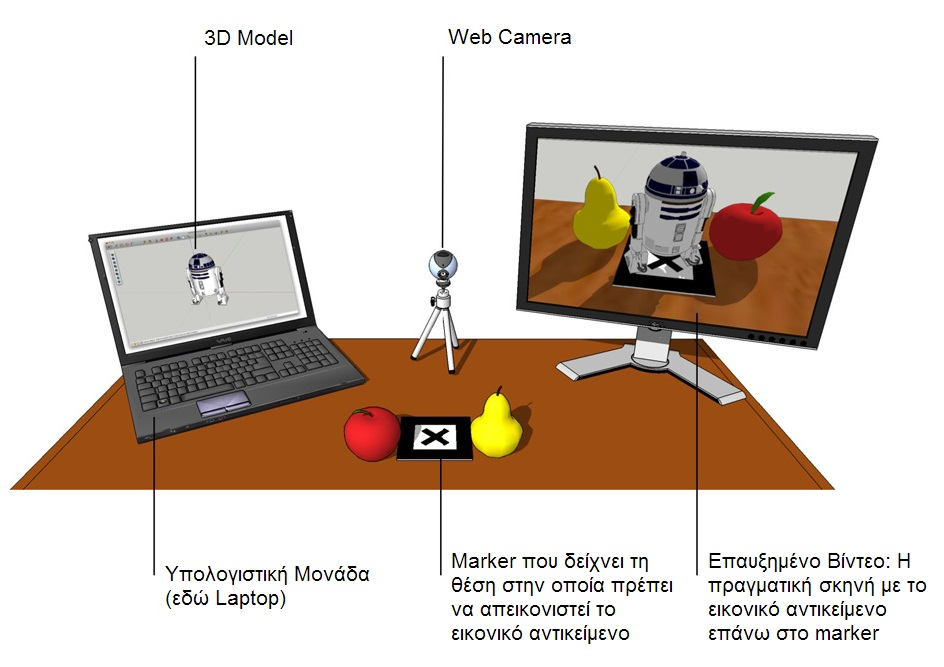
\includegraphics[scale=0.25, angle=0]{Files/Figures/ar_system_example.jpg}
    \caption[Παράδειγμα εγκατάστασης ενός συστήματος επαυξημένης πραγματικότητας ]{ Παράδειγμα εγκατάστασης ενός συστήματος επαυξημένης πραγματικότητας \cite{ar_example}}
    \label{fig:ar_example}
\end{figure}


Η κύρια διαδικασία για τη σωστή λειτουργία ενός συστήματος επαυξημένης πραγματκότητας έχει να κάνει με το κομμάτι της ανίχνευσης. Το κομμάτι αυτό ασχολείται με τον υπολογισμό της σχετικής πόζας της κάμερας σε πραγματικό χρόνο. Με τον όρο πόζα (pose) περιγράφουμε τους 6 βαθμούς ελευθερίας της τοποθεσίας ενός αντικειμένου, δηλαδή τη θέση του στον τρισδιάστατο χώρο και τον προσανατολισμό στον τριασδιάστατο χώρο.

Η διαδικασία της ανίχνευσης είναι αυτή που επιτρέπει την προσθήκη εικονικών αντικειμένων σε μία πραγματική σκηνή.
Η βασική διαφορά σε σύγκριση με άλλα εργαλεία επεξεργασίας εικόνας παρατηρείται στο γεγονός ότι στην επαυξημένη πραγματικότητα τα εικονικά αντικείμενα μετακινούνται και περιστρέφονται σε 3 διαστάσεις αντί για 2 όπως γίνεται συνήθως σε εικόνες.  Ο απλούστερος τρόπος εκτίμησης της πόζας είναι η χρήση δεικτών (markers). 
Ωστόσο, το μαθηματικό μοντέλο ( προβολική γεωμετρία) πίσω από τις μεθόδους υπολογισμού της πόζας είναι το ίδιο. 

Παρόμοια προβλήματα βελτιστοποίησης διαμορφώνονται σε διαφορετικές μεθόδους υπολογισμού της πόζας και λύνονται με τις ίδιες μεθόδους βελτιστοποίησης.  
Μπορούμε να θεωρήσουμε ότι οι markers είναι ένας ειδικός τύπος χαρακτηριστικού και επομένως μπορούμε να ορίσουμε μεθόδους με βάση την ανίχνευση markers και μετέπειτα μεθόδους με βάση την ανίχνευση χαρακτηριστικών, καθώς και υβριδικές μεθόδους. Στη συγκεκριμένη διπλωματική εργασία θα επικεντρωθούμε σε συστήματα επαυξημένης πραγματικότητας που βασίζονται σε markers.

Συνήθως η καταγραφή της εικόνας δεν είναι σημαντικό κομμάτι στην επαυξημένη πραγματικότητα. Συνήθως χρησιμοποιούνται έτοιμες βιβλιοθήκες για το σκοπό αυτό,

Τα εργαλεία και οι βιβλιοθήκες επαυξημένης πραγματικότητας παρέχουν υποστήριξη για την καταγραφή εικόνας και βίντεο. Η διαδικασία τηςα απεικόνισης ζωγραφίζει την εικονική εικόνα πάνω στην εικόνα του βίντεο. Στα γραφικά υπολογιστών, η εικονική σκηνή προβάλλεται πάνω στο επίπεδο της εικόνας χρησιμοποιώντας μία εικονική κάμερα και αυτή η προβολή απεικονίζεται στο τέλος. 

Απαιτείται ουσιαστικά η χρήση μίας εικονικής κάμερας που είναι παρόμοια με τη πραγματική κάμερα του συστήματος. Με αυτό τον τρόπο τα εικονικά αντικείμενα προβάλλονται στη σκηνή με τον ίδιο τρόπο με τον οποίο θα προβάλλονταν πραγματικά αντικείμενα και το αποτέλεσμα είναι γεωμετρικά πειστικό. Για να μπορέσουμε να μιμηθούμε τις ιδιότητες της πραγματικής κάμερας, το σύστημα πρέπει να ξέρει τα οπτικά χαρακτηριστικά της κάμερας. Η διαδικασία κατά την οποία προσδιορίζονται αυτά τα χαρακτηριστικά ονομάζεται βαθμονόμηση κάμερας.

Η βαθμονόμηση της κάμερας μπορεί να είναι μέρος του συστήματος επαυξημένης πραγματικότητας ή ξεχωριστή διαδικασία. Πολλές βιβλιοθήκες παρέχουν εργαλεία βαθμονόμησης, όπως για παράδειγμα οι βιβλιοθήκες ArUco, ALVAR, ARToolkit.


Ωστόσο για τη διαδικασία της βαθμονόμησης μπορούν να χρησιμοποιηθούν και τρίτα εργαλεία βιβλιοθηκών όπως το Matlab ή η OpenCV. 

Στην εργασία αυτή αφού περιγράψουμε τη διαδικασία της βαθμονόμησης, θεωρούμε ότ έχουμε πάντα μία σωστά βαθμονομημένη κάμερα για την ανάπτυξη της εφαρμογής μας.

Η ποικιλία των συσκευών οι οποίες υποστηρίζουν συστήματα επαυξημένης πραγματικότητας είναι μεγάλη και περιλαμβάνει σταθερούς και φορητούς υπολογιστές, tablets, κινητά και άλλες υπολογιστικές μονάδες. Ανάλογα με την εφαρμογή, μπορεί να αξιοποιηθεί η ενσωματωμένη κάμερα της συσκευής, μία απλή USC κάμερα, μία Firewire κάμερα ή μία ψηφιακή κάμερα. Μπορεί επίσης να χρησιμοποιηθεί μία συσκευή απεικόνισης που προσαρτάται στο κεφάλι του χρήστη(HMD), μία συσκευή απεικόνισης οπτικής τεχνολογίας ή η ίδια η οθόνη της υπολογιστικής μονάδας. Επίσης μπορεί το σύστημα να προβάλλει την επαυξημένη σκηνή στον πραγματικό κόσμο\cite{jones2013illumiroom} ή να χρησιμοποιηθεί μια στερεοσκοπική συσκευή απεικόνισης. Η κατάλληλη εγκατάσταση εξαρτάται από την εφαρμογή και το περιβάλλον στο οποίο αναπτύσσεται.









Ο συνδυασμός πραγματικών και εικονικών εικόνων σε μία συγχωνευμένη εικόνα παρουσιάζει τεχνικές δυσκολίες για τους σχεδιαστές εφαρμογών επαυξημένης πραγματικότητας.  Το ερώτημα, στο οποίο καλούνται να απαντήσουν, έχει να κάνει με το πώς θα πραγματοποιηθεί η συνένωση των δύο εικόνων. Στην ενότητα αυτή παρουσιάζονται τα είδη τεχνολογιών θέασης της επαυξημένης σκηνής \cite{azuma1997} \cite{Vallino1998}  \cite{azuma2001}.





-Head-Worn Displays (HWDs)
Οι συσκευές αυτές, γνωστές ως Head-Worn Displays (HWD) ή Head-Attached Displays, φοριούνται στο κεφάλι του χρήστη ή σε κάποιο μέρος του κεφαλιού. Στις παρακάτω παραγράφους περιγράφονται οι κυριότερες κατηγορίες των συσκευών αυτών.\cite{barfield2001fundamentals}


Στην επαυξημένη πραγματικότητα υπάρχουν δύο βασικές κατηγορίες συστημάτων απεικόνισης που αξιοποιούν τα HMDs ως μέσο για την οπτική διεπαφή. 

Επιτυγχάνεται τοποθετώντας οπτικούς μπροστά από τα μάτια του χρήστη. Κάθε σύστημα έχει συγκεκριμένα πλεονεκτήματα και μειονεκτήματα, που σχετίζονται με το σχεδιασμό μιας εφαρμογής και είναι απαραίτητο  να θεωρήσουμε όλες τις παραμέτρους πριν την υλοποίηση του συστήματος AR.Αξίζει να σημειωθεί ότι τα non-immersive HMDs μπορεί να είναι μονοσκοπικά ή στερεοσκοπικά. Οι διαφορές ανάμεσα τους πρέπει να εξεταστούν όταν γίνεται η επιλογή του σχεδιασμού με βάση ένα optical based system. Οι οπτικές προσεγγίσεις είναι απλούστερες και φθηνότερες. Ο κόσμος φαίνεται μέσα από οπτικούς combiners,οπότε υπάρχει μόνο ένα video stream να ανησυχούμε. Στα see-through systems η μόνη διαθέσιμη πληροφορία είναι η θέση της κεφαλής του χρήστη που προέρχεται από έναν head tracker. 



Για την ενίσχυση της "εμβύθισης" του χρήστη χρειάζονται διάφορες τεχνολογίες απεικόνισης της επαυξημένης σκηνής. Τα HMDs έχουν ευρεία χρήση σε εφαρμογές εικονικής πραγματικότητας. Ένα σύστημα Head-Mounted Display (HMD) είναι μία συσκευή που προσαρτάται στο κεφάλι του χρήστη και συνδυάζει την εικόνα του πραγματικού κόσμου με εικονικά αντικείμενα, μέσω χρήσης οπτικής ή βίντεο τεχνολογίας. 
Στο πεδίο της επαυξημένης πραγματικότητας χρησιμοποιούνται 2 είδη HMD. Συγκεκριμένα τα video see-through and optical see-through. Ο όρος “see-through” προέρχεται από την ανάγκη του χρήστη να μπορεί να βλέπει τον πραγματικό κόσμο που βρίσκεται μπροστά του, ακόμα και όταν φοράει το HMD.

 
\textbf{Optical See-Through Displays}


Η τεχνολογία αυτή βασίζεται στη δημιουργία ενός συστήματος παρουσίασης το οποίο προσαρτάται στο κεφάλι του χρήστη (optical see-through HMDs) που απαιτεί την τοποθέτηση "οπτικών συνδυαστών" (συνήθως ημιδιαπερατών και ημιανακλαστικών κάτοπτρων ) μπροστά από τα μάτια του χρήστη, που του επιτρέπουν να δει τόσο το πραγματικό περιβάλλον γύρω του, όσο και τα εικονικά αντικείμενα που παράγονται από τον υπολογιστή. 
Τα εικονικά αντικείμενα ανακλούνται μέσω των κατόπτρων από τις οθόνες που είναι προσαρτημένες στο κεφάλι του, με βάση την τρέχουσα θέση του, όπως φαίνεται στην εικόνα ~\ref{fig:videoseethrough} ).  Επομένως, όταν οι χρήστες μετακινούν τα κεφάλια τους, τα εικονικά αντικείμενα διατηρούν τη θέση τους στον κόσμο σαν να ήταν κομμάτι του πραγματικου περιβάλλοντος.



Τα optical see-through συστήματα δε χρησιμοποιούν καθόλου την είσοδο του σήματος βίντεο, με αποτέλεσμα ο χρήστη να βλέπει το πραγματικό περιβάλλον, και όχι μία αναπαράσταση μέσω βίντεο, πετυχαίνοντας την αξιοποίηση της υψηλής ανάλυσης του πραγματικού κόσμου όπως τον παρατηρεί ο χρήστης. Ουσιαστικά, η συγχώνευση του πραγματικού κόσμου με την εικονική επαύξηση γίνεται οπτικά μπροστά από το χρήστη \cite{Vallino1998} . Αυτή η τεχνολογία είναι παρόμοια με τα  heads up displays (HUD) που χρησιμοποιούνται στα cockpits μαχητικών αεροσκαφών και παρουσιάστηκαν στην προηγούμενη ενότητα~\ref{sec:apps}

Επιπλέον παρουσιάζουν ορισμένα πλεονεκτήματα. Αρχικά θεωρούνται ασφαλή διότι οι χρήστες μπορούν να δουν τη πραγματική σκηνή που βρίσκεται μπροστά τους, ακόμα και αν υπάρξει σφάλμα στην παροχή ισχύος, με αποτέλεσμα η συγκεκριμένη τεχνολογία να είναι ιδανική για στρατιωτικούς και ιατρικούς σκοπούς. Ωστόσο, κι άλλες συσκευές εισόδου όπως κάμερες είναι απαραίτητες για αλληλεπίδραση και registration. Επιπλέον παρουσιάζουν χαμηλό κόστος, και δεν επηρεάζονται από το πρόβλημα της παράλλαξης το οποίο δημιουργεί μία διαφορά ως προς τη θέση των ματιών και της κάμερας \cite{krevelen2010} .


Εφόσον οι χρήστες βλέπουν την πραγματική σκηνή, το εικονικό μέρος είναι ο μόνος λόγος που προκαλείται καθυστέρηση(lag). Για τον ίδιο λόγο, η ποιότητα της σκηνής της προβολής του κόσμου είναι πολύ καλύτερη από την αναπαράσταση μέσω βίντεο. Επομένως η χρήση ενός see-through system εξαλείφει το πρόβλημα της καθυστέρησης του συστήματος και βελτιώνει την ποιότητα προβολής της επαυξημένης σκηνής. 


Ωστόσο πέρα από πλεονεκτήματα, ο συνδυασμός εικονικών αντικειμένων ολογραφικά μέσα από κάτοπτρα και φακούς δημιουργεί και μειονεκτήματα, καθώς μειώνεται η φωτεινότητα, αλλά και η αίσθηση "εμβύθισης" του χρήστη. Επομένως η συγκεκριμένη τεχνική φαίνεται ακατάλληλη για εξωτερική χρήση. Παράλληλα, μία σημαντική παράμετρος, αυτή του πεδίου όρασης του χρήστη (field-of-view) περιορίζεται και μπορεί να προκληθεί ψαλιδισμός των εικονικών εικόνων στα άκρα των ανακλαστήρων. Τέλος, η απόκρυψη των πραγματικών αντικειμένων (occlusion) είναι δυσκολότερη επειδή το φως συνδυάζεται πάντα με την εικονική εικόνα. 

Επιπλέον το γεγονός ότι δεν υπάρχει σήμα βίντεο, αφού δεν υπάρχει κάμερα. Επομένως οι αισθητήρες θέσης μέσα στο HMD είναι ο μόνος τρόπος να εξάγουμε πληροφορίες της πόζας για λόγους registration. Αυτό έχει σαν συνέπεια τη μείωση της ακρίβειας του registration, αν η επιλεγμένη μέθοδος head tracking που χρησιμοποιείται δεν είναι απόλυτα ακριβής \cite{Malik2002} .

H ποιότητα της εικονικής επαύξησης είναι συνήθως χαμηλή, αφού ο μικρός οπτικός συνδυαστής μπροστά από το μάτι του χρήστη είναι χαμηλής ανάλυσης. Έτσι περιορίζεται η εμφάνιση την εμφάνιση των λεπτομερειών των γραφικών που προβάλλονται στην έξοδο. Η ποιότητα των εικονικών αντικειμένων περιορίζεται από την ταχύτητα επεξεργασίας και τις γραφικές ικανότητες του συστήματος επαύξησης. Επομένως η δημιουργία πειστικών επαυξήσεων γίνεται δυσκολότερη αφού ο πραγματικός κόσμος θα εμφανίζεται κανονικά, σε αντίθεση με τα εικονικά αντικείμενα που θα εμφανίζονται pixilated. Αν ένα σύστημα επαυξημένης πραγματικότητας απαιτεί εικονικά αντικείμενα με γραφικά υψηλής ανάλυσης, τότε προτιμώνται συνήθως συστήματα video see-through ή monitor-based \cite{Mcdonald2003} . 


\begin{figure}[H]
    \centering
    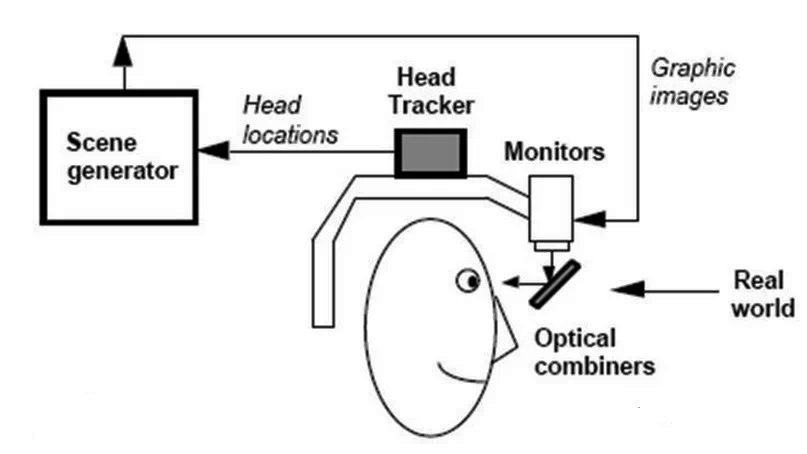
\includegraphics[scale=0.7, angle=0]{Files/Figures/optical.jpg}
    \caption[Διάγραμμα συστήματος Optical See-Through Display \cite{azuma1997}]{ Διάγραμμα συστήματος Optical See-Through Display \cite{azuma1997}}
    \label{fig:opticalseethrough}
\end{figure}



\textbf{Video See-Through Displays}

Τα HMDs που χρησιμοποιούν βίντεο τεχνολογία (video see-through HMDs), συνδυάζουν ένα «κλειστό» HMD (closed-view HMD) και μία ή δύο βιντεοκάμερες προσαρτημένες στο κεφάλι του χρήστη, όπως φαίνεται στην εικόνα ~\ref{fig:videoseethrough} . Η σκηνή του πραγματικού κόσμου καταγράφεται από τις βιντεοκάμερες, οι οποίες του παρέχουν τη δυνατότητα να βλέπει τον πραγματικό κόσμο. Με αυτό τον τρόπο, ο χρήστης δε βλέπει τον πραγματικό κόσμο απευθείας, αλλά αντίθετα βλέπει μόνο αυτό που απεικονίζεται στις μικρές οθόνες στο εσωτερικό του HMD.  

 

Το πλεονέκτημα των συστημάτων τέτοιου τύπου παρατηρείται στο ότι κατά τη καταγραφή της πραγματικής σκηνής μέσω βίντεο, μπορούν να εξαχθούν πληροφορίες για τη σκηνή. Οι ψηφιοποιημένες εικόνες επιτρέπουν την ανίχνευση της κίνησης του κεφαλιού του χρήστη παρέχοντας μεγαλύτερη ακρίβεια κατά τη διαδικασία του tracking της θέσης του κεφαλιού και επομένως οδηγεί σε πιο ακριβές registration. Επιπλέον η απεικόνιση του βίντεο είναι συνήθως υψηλής ανάλυσης και δίνεται η δυνατότητα να απεικονιστούν τα εικονικά αντικείμενα με λεπτομερή γραφικά σε συνδυασμό με το βίντεο εισόδου.Συνεπώς, αυξάνεται η ρεαλιστικότητα και η εμβύθιση του χρήστη που μπορεί να προσφέρει ο επαυξημένος κόσμος \cite{krevelen2010} .


Αυτή η διαδικασία συγχώνευσης προσθέτει ωστόσο καθυστερήσεις στο σύστημα. Οι καθυστερήσεις του συστήματος λόγω της καταγραφής, της επεξεργασίας, της επαύξησης και της απεικόνισης σε κάθε frame του βίντεο μεταφράζεται σε lag που καταλαβαίνει ο χρήστης με αποτέλεσμα να χάνεται η αίσθηση της εμβύθισης. Αυτό είναι ένα μειονέκτημα στα συστήματα video see-through technology που δεν μπορεί να αποφευχθεί αλλά μπορεί να ελαχιστοποιηθεί. Μειονεκτήματα εντοπίζονται επίσης στη χαμηλή ανάλυση απεικόνισης του πραγματικού κόσμου, στο περιορισμένο field-of-view (αν και μπορεί να αυξηθεί εύκολα), και τον αποπροσανατολισμό των χρηστών λόγω της παράλλαξης (eye-offset) λόγω της θέσης της κάμερας σε μία απόσταση από τη πραγματική θέση των ματιών του χρήστη. Τέλος, μία μεγάλη διαφορά ανάμεσα στις κάμερες και τα μάτια του χρήστη, μπορεί να ελλατώσει την αίσθηση της εμβύθισης, αφού τα πάντα στις σκηνές που καταγράφονται θα μετατοπιστούν ψηλότερα ή χαμηλότερα από εκεί που θα έπρεπε να είναι(ως προς την κανονικό επίπεδο της θέσης των ματιών) \cite{Malik2002} . 



\begin{figure}[H]
    \centering
    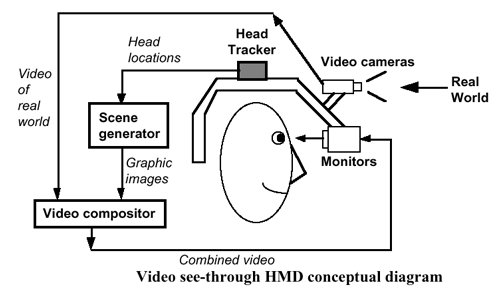
\includegraphics[scale=0.8, angle=0]{Files/Figures/videoseethrough.jpg}
    \caption[Διάγραμμα συστήματος Video See-Through Display \cite{azuma1997}]{ Διάγραμμα συστήματος Video See-Through Display \cite{azuma1997}}
    \label{fig:videoseethrough}
\end{figure}


\textbf{Monitor-based Systems}


Πέρα όμως από τις συσκευές τεχνολογίας HMD, υπάρχουν και συσκεύες απεικόνισης σε οθόνη με χρήση βίντεο-τεχνολογίας. Οι συσκευές αυτές απεικονίζουν τις επαυξημένες σκηνές σε μία κοινή οθόνη, κάνοντας χρήση της επεξεργασίας εικόνας και της μίξης του εικονικού με το πραγματικό. Η απλούστερη προσέγγιση ενός monitor-based συστήματος απεικόνισης, φαίνεται στο~\ref{fig:monitor} .

Το είδος αυτό της επαυξημένης πραγματικότητας αποτελεί μία από τις πιο απλές και αποδοτικές λύσεις, καθώς απαιτεί έναν τυπικό ηλεκτρονικό υπολογιστή και  και μία βιντεοκάμερα USB ή Firewire. Ωστόσο αυτή η απλότητα προκαλεί συνέπειες στον τομέα της εμβύθισης του χρήστη σε περιβάλλοντα επαυξημένης πραγματικότητας, λόγω του σχετικά μικρού μεγέθους της οθόνης και του συνακόλουθου μικρού οπτικού πεδίου. Το σύστημα επαύξησης μπορεί να χρησιμοποιήσει τεχνικές με βάση την όραση υπολογιστών για να υπολογίσει τις πληροφορίες της πόζας(θέση και προσανατολισμός) του χρήστη για σκοπούς registration (ανιχνεύοντας χαρακτηριστικά ή πρότυπα για παράδειγμα).

Ακόμη, μειονέκτημα αποτελεί η ποιότητα της εικόνας, καθώς αυτή περιορίζεται από την ανάλυση της κάμερας. Προφανώς, το να βλέπει κάποιος τον πραγματικό κόσμο μέσα από τη μικρή οθόνη ενός υπολογιστή περιορίζει το ρεαλισμό και την φορητότητα του επαυξημένου κόσμου. Επιπλέον, εφόσο κάθε frame της κάμερας χρειάζεται επεξεργασία από το σύστημα επαύξησης, μπορεί να καταγραφεί καθυστέρηση λόγω του χρόνου από τη στιγμή που καταγράφεται η πραγματική σκηνή, μέχρι να απεικονιστεί η τελική επαυξημένη εικόνα. 




\begin{figure}[H]
    \centering
    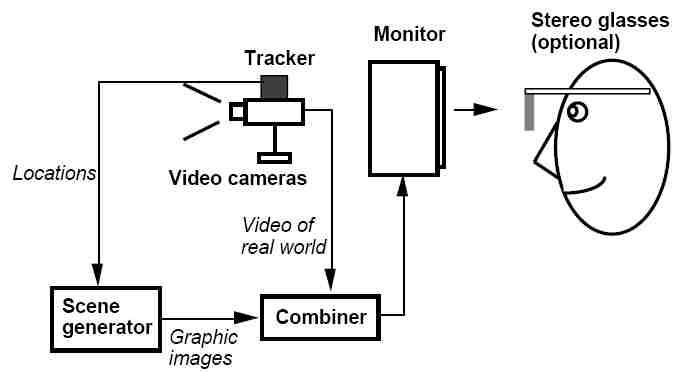
\includegraphics[scale=0.8, angle=0]{Files/Figures/monitor.jpg}
    \caption[Διάγραμμα συστήματος Monitor Display \cite{azuma1997}]{ Διάγραμμα συστήματος Monitor Display \cite{azuma1997}}
    \label{fig:monitor}
\end{figure}


\begin{figure}[H]
    \centering
    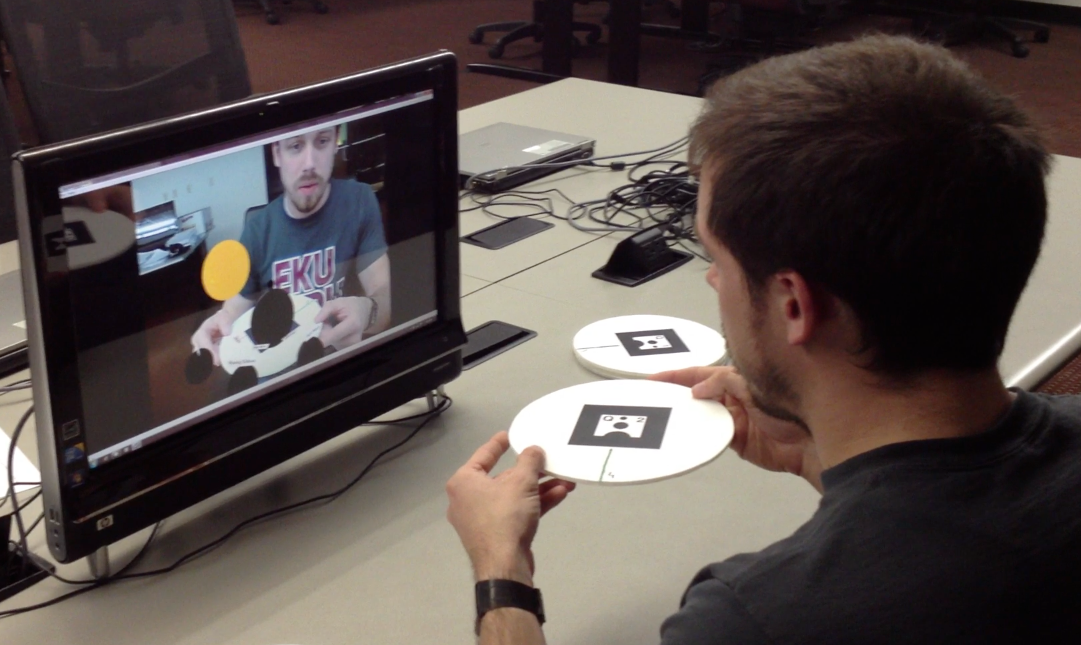
\includegraphics[scale=0.2, angle=0]{Files/Figures/monitor_example.png}
    \caption[Παράδειγμα εφαρμογής μέσω συσκευής απεικόνισης σε
οθόνη \cite{monitor_ar} .]{ Παράδειγμα εφαρμογής μέσω συσκευής απεικόνισης σε
οθόνη \cite{monitor_ar} .}
    \label{fig:monitor_example}
\end{figure}


\textbf{Φορητές Συσκευές}


Οι συσκευές αυτές, ευρέως γνωστές ως Handheld Displays (HDs), περιλαμβάνουν μία οθόνη, μέσω της οποίας είναι δυνατή η θέαση της επαυξημένης σκηνής, και είναι φορητές, μικρού μεγέθους, έτσι ώστε ο χρήστης να μπορεί να τις κρατήσει στο χέρι του και να τις μεταφέρει μαζί του. 

Τέτοιες συσκευές είναι τα κινητά τηλέφωνα – και συγκεκριμένα τα «έξυπνα» κινητά τηλέφωνα, γνωστά ως smartphones – τα tablet PCs και οι – λιγότερο χρησιμοποιούμενοι πλέον – προσωπικοί ψηφιακοί οδηγοί PDAs (Personal Digital Assistants). 

Στη μεγάλη πλειονότητα των εφαρμογών επαυξημένης πραγματικότητας που προορίζονται για φορητές συσκευές χειρός, η βιντεοκάμερα «αιχμαλωτίζει» τη ζωντανή εικόνα του πραγματικού περιβάλλοντος, η οποία επαυξάνεται με επιπρόσθετες γραφικές πληροφορίες πριν την απεικόνισή της στην οθόνη. 

Μέσω των συσκευών αυτών, ο χρήστης δεν «βυθίζεται» στο επαυξημένο περιβάλλον, αλλά το παρακολουθεί μέσω της οθόνης της συσκευής του, γεγονός το οποίο θα μπορούσε να θεωρηθεί ως μειονέκτημα. 

Επίσης, η συνήθως χαμηλή επεξεργαστική ισχύ και μνήμη τους, μπορεί να προκαλέσει καθυστερήσεις κατά την εκτέλεση της εφαρμογής. Ωστόσο οι συσκευές αυτές παρουσιάζουν το πλεονέκτημα του μικρότερου μεγέθους και βάρους \cite{wagner2007handheld} \cite{arth2015history} .

Τα τελευταία χρόνια έχουν αναπτυχθεί και σύγχρονα συστήματα απεικόνισης όπως ειδικοί φακοί επαφής, ωστόσο δε θα αναφέρουμε περισσότερα για τη συγκεκριμένη τεχνολογία.





\section{Marker-based Tracking}
%MONO FIDUCIAL MARKER TRACKING

%eisagogi enotitas
While some approaches seek natural features such as key points or textures,fiducial markers are still an attractive approach because they are easy to detect and high speed, as well as precision may be achieved.


Σε αυτό το κεφάλαιο γίνεται μία εισαγωγή στις μαθηματικές έννοιες της επαυξημένης πραγματικότητας, στις μεθόδους που χρησιμοποιούνται και στην αναγνώριση δεικτών.  
In this chapter, we review prior work in the field of augmented reality from which our research draws upon. We start by providing an introduction to the mathematical concepts of augmented reality, and describe how they relate to the registration problem. We then present a brief survey of various proposed solutions to the registration problem in the current augmented reality literature. We conclude by briefly describing some open issues.




Η επαυξημένη πραγματικότητα παρουσιάζει πληροφορίες στα πλαίσια του πραγματικού κόσμου. Για να συμβεί αυτό, το σύστημα πρέπει να γνωρίζει που βρίσκεται ο χρήστης και προς τα που κοιτά σε κάθε χρονική στιγμή. Συνήθως ο χρήστης εξερευνεί το περιβάλλον μέσα από μία οθόνη που απεικονίζει την εικόνα που καταγράφει η κάμερα μαζί με την επαυξημένη πληροφορία.  
Επομένως, το σύστημα χρειάζεται πρακτικά να ξέρει τη θέση και τον προσανατολισμό της κάμερας, έτσι ώστε να απεικονίσει τα εικονικά αντικείμενα στη σωστή θέση. Αυτή η διαδικασία ονομάζεται tracking και αναφέρεται στον υπολογισμό της σχετικής πόζας(pose) της κάμερας (θέση και προσανατολισμός) σε πραγματικό χρόνο και είναι ένα από τα βασικότερα μέρη ανάπτυξης εφαρμογών επαυξημένης πραγματικότητας.


Οι ερευνητές στα πεδία της όρασης υπολογιστών έχουν αναπτύξει έναν αξιοσημείωτο αριθμό μεθόδων tracking. Οι μέθοδοι αυτές μπορούν να ταξινομηθούν με βάση τον εξοπλισμό που χρησιμοποιείται σε μεθόδους sensor tracking, visual tracking και υβριδικές. Εφόσον στα περισσότερα συστήματα επαυξημένης πραγματικότητας χρησιμοποιείται συνήθως μία κάμερα, οι τεχνικές visual tracking είναι αυτές που παρουσιάζουν μεγαλύτερο ενδιαφέρον, οπότε θα επικεντρωθούμε σε αυτές.


Στα συστήματα visual tracking, η πόζα της κάμερας μπορεί να υπολογιστεί με βάση την παρατήρηση των σκηνών που καταγράφει. Σε ένα άγνωστο περιβάλλον, παρατηρούνται πολλές δυσκολίες, καθώς απαιτείται αρκετός χρόνος προκειμένου να γίνει η συλλογή αρκετών δεδομένων για τον υπολογισμό της πόζας και επιπλέον, η εκτίμηση των υπολογισμών ολισθαίνει με την πάροδο του χρόνου. Καθώς το περιβάλλον δεν είναι γνωστό στο σύστημα, ο προσανατολισμός του άξονα συντεταγμένων επιλέγεται τυχαία, κάτι το οποίο μπορεί να μην είναι ιδιαίτερα βολικό για το χρήστη. Επιπλέον, είναι αδύνατο να υπολογιστεί η σωστή κλίμακα μόνο με βάση τις οπτικές παρατηρήσεις. Μία λύση που θα μπορούσε να ξεπεράσει αυτές τις δυσκολίες, εντοπίζεται στην εισαγωγή ενός ανιχνεύσιμου προκαθορισμένου στόχου στο περιβάλλον και στη χρήση τεχνικών όρασης υπολογιστών για τον εντοπισμό του στη σκηνή. 

Ο στόχος αυτός είναι ουσιαστικά ένας δείκτης ή marker, ένα σημάδι ή μια εικόνα, που μπορεί να εντοπιστεί από ένα υπολογιστικό σύστημα μέσω του βίντεο χρησιμοποιώντας τεχνικές επεξεργασίας εικόνας, αναγνώρισης προτύπων και υπολογιστικής όρασης (π.χ~\ref{fig:marker})). Μόλις εντοπιστεί ένας marker, μπορεί να οριστεί η σωστή θέση και ο προσανατολισμός της κάμερας. Αυτή η προσέγγιση ονομάζεται ανίχνευση βασισμένη σε marker (marker-based tracking) και χρησιμοποιείται ευρύτατα στην επαυξημένη πραγματικότητα.%vale link

\begin{figure}[H]
    \centering
    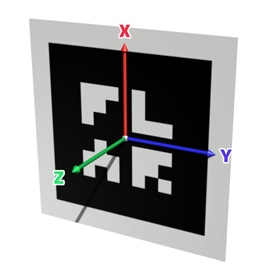
\includegraphics[scale=0.6, angle=0]{Files/Figures/marker-axis.jpg}
    \caption[Παράδειγμα marker]{ Παράδειγμα marker}
    \label{fig:marker}
\end{figure}




Άλλες προσεγγίσεις χρησιμοποιούν ανίχνευση με βάση τον εντοπισμό οπτικών χαρακτηριστικών και εντοπισμό προκαθορισμένων μοντέλων. Στον εντοπισμό με βάση προκαθορισμένα μοντέλα, το σύστημα γνωρίζει εκ των προτέρων τις ιδιότητες ενός μοντέλου ή μέρους της σκηνής (π.χ CAD μοντέλο). Πραγματοποιείται σύγκριση ανάμεσα στα frames που κταγράφονται και γίνεται προσπάθεια να γίνει αντιστοίχηση του μοντέλου με ένα μέρος της σκηνής. Μόλις συμβεί αυτό, μπορεί να υπολογιστεί και η πόζα της κάμερας. Στη διαδικασία feature-based tracking,το σύστημα προσπαθεί να ανιχνεύσει οπτικά χαρακτηριστικά της σκηνής μέσα από τις εικόνες και να γνωρίσει το περιβάλλον με βάση ορισμένες παρατηρήσεις κινήσεων ανάμεσα σε διαδοχικά frames. Αν και η επικρατούσα τάση στην έρευνα σχετικά με το visual tracking τείνει προς το feature-based tracking, που δεν απαιτεί την εκτύπωση και χρήση markers, οι μέθοδοι που βασίζονται σε markers παρουσιάζουν καλύτερες επιδόσεις από τις μεθόδους feature-based σε συγκεκριμένες περιπτώσεις και χρησιμοποιούνται ακόμα πολύ συχνά σε εφαρμογές επαυξημένης πραγματικότητας \cite{wagner2008robust} \cite{rabbi2014applications} .


Η ευρεία χρήση συστημάτων που λειτουργούν με βάση την ανίχνευση markers εξηγείται και από το γεγονός ότι είναι εύκολα στην υλοποίηση και υπάρχουν πολλά διαθέσιμα εργαλεία για την ανάπτυξη τέτοιων εφαρμογών (π.χ ARToolKit \cite{artoolkit}, ALVAR \cite{alvar}, ArUco \cite{aruco}). Τα εργαλεία αυτά αποτελούν μία καλή βάση για να ξεκινήσει κάποιος την ανάπτυξη εφαρμογών επαυξημένης πραγματικότητας. Επιπλέον, οι markers παρέχουν εκτιμήσεις για τη σωστή κλίμακα και βολικές συντεταγμένες για κάθε frame όπως αναφέρθηκε και προηγουμένως. Μπορούν να κωδικοποιήσουν πληροφορίες ή να έχουν απλά ένα ID. Κάτι τέτοιο, επιτρέπει στο σύστημα να επισυνάψει συγκεκριμένα αντικείμενα ή αλληλεπιδράσεις στα markers. Στη συστήματα που χρησιμοποιούν marker-based tracking, απαιτείται η ανίχνευση του marker, η ταυτοποίηση του και ο υπολογισμός της πόζας. 

Στις παρακάτω ενότητες, παρουσιάζεται η διαδικασία υπολογισμού της πόζας ενός δείκτη. Αρχικά παρουσιάζονται περιληπτικά οι βασικές αρχές της προβολικής γεωμετρίας και το μοντέλο κάμερας pinhole. Ύστερα αναλύεται η διαδικασία βαθμονόμησης κάμερας με αποτέλεσμα τον υπολογισμό των παραμέτρων της και ο τρόπος ανίχνευσης ενός marker. Στο τέλος της ενότητας παρουσιάζεται ένας τρόπος αξιοποίησης πολλαπλών markers με στόχο τη βελτίωση της επίδοσης του συστήματος.





Στη συνέχεια του κεφαλαίου θα χρησιμοποιήσουμε ομογενείς συντεταγμένες. Οι ομογενείς συντεταγμένες (homogeneous coordinates) είναι ένα είδος συντεταγμένων που χρησιμοποιείται στην προβολική γεωμετρία, αντίστοιχα με τις καρτεσιανές συντεταγμένες που χρησιμοποιούνται στην ευκλείδεια γεωμετρία. Στα πλεονεκτήματά τους συγκαταλέγονται η δυνατότητα αναπαράστασης όλων των σημείων, ακόμα και των σημείων του απείρου, με πεπερασμένες συντεταγμένες, καθώς και η δυνατότητα έκφρασης ενός προβολικού μετασχηματισμού με τη βοήθεια ενός μόνο πίνακα.

Πιο συγκεκριμένα, έστω ένα σημείο της εικόνας με καρτεσιανές συντεταγμένες \[\begin{bmatrix} x \\ y \end{bmatrix}\]
Το αντίστοιχο σημείο, σε ομογενείς συντεταγμένες μπορεί να αναπαρασταθεί ως: \[\begin{bmatrix} wx \\ wy \\ w\end{bmatrix}=
\begin{bmatrix}x'\\y'\\w\end{bmatrix} , w\neq0 \].

Ομοίως στον 3D χώρο ένα σημείο με καρτεσιανές συντεταγμένες \[\begin{bmatrix} x \\ y \\ z \end{bmatrix}\] μπορεί να αναπαρασταθεί ως: \[\begin{bmatrix} wx \\ wy \\ wz \\ w\end{bmatrix}=
\begin{bmatrix}x'\\y'\\z' \\ w\end{bmatrix} , όπου w\neq0 \].


Παρά το γεγονός ότι μπορεί να χρησιμοποιηθεί ένας οποιοσδήποτε μη μηδενικός αριθμός $w$, συνήθως παίρνουμε $w=1$, ώστε η αλλαγή συστήματος συντεταγμένων να γίνεται ευκολότερα.

Ο παρακάτω πίνακας συνοψίζει την αναπαράσταση των σημείων που θα χρησιμοποιηθεί:




\begin{tabu} to 0.9\textwidth { | X[l] | X[c,m] | X[c,m] | }
   \hline
    & Ευκλείδεια Γεωμετρία & Προβολική Γεωμετρία \\[0.5cm]
   \hline
   Σημείο στο 2Δ Χώρο  & $\begin{bmatrix} x \\ y\end{bmatrix}$  & $\begin{bmatrix} x \\ y\end{bmatrix}$  \\[1cm]
   \hline
   Σημείο στο 2Δ Χώρο  & $\begin{bmatrix} x \\ y\end{bmatrix}$  & $\begin{bmatrix} x \\ y\end{bmatrix}$  \\[1cm]
   \hline
\end{tabu}



\subsection{Ανίχνευση Marker}



\begin{figure}[H]
    \centering
    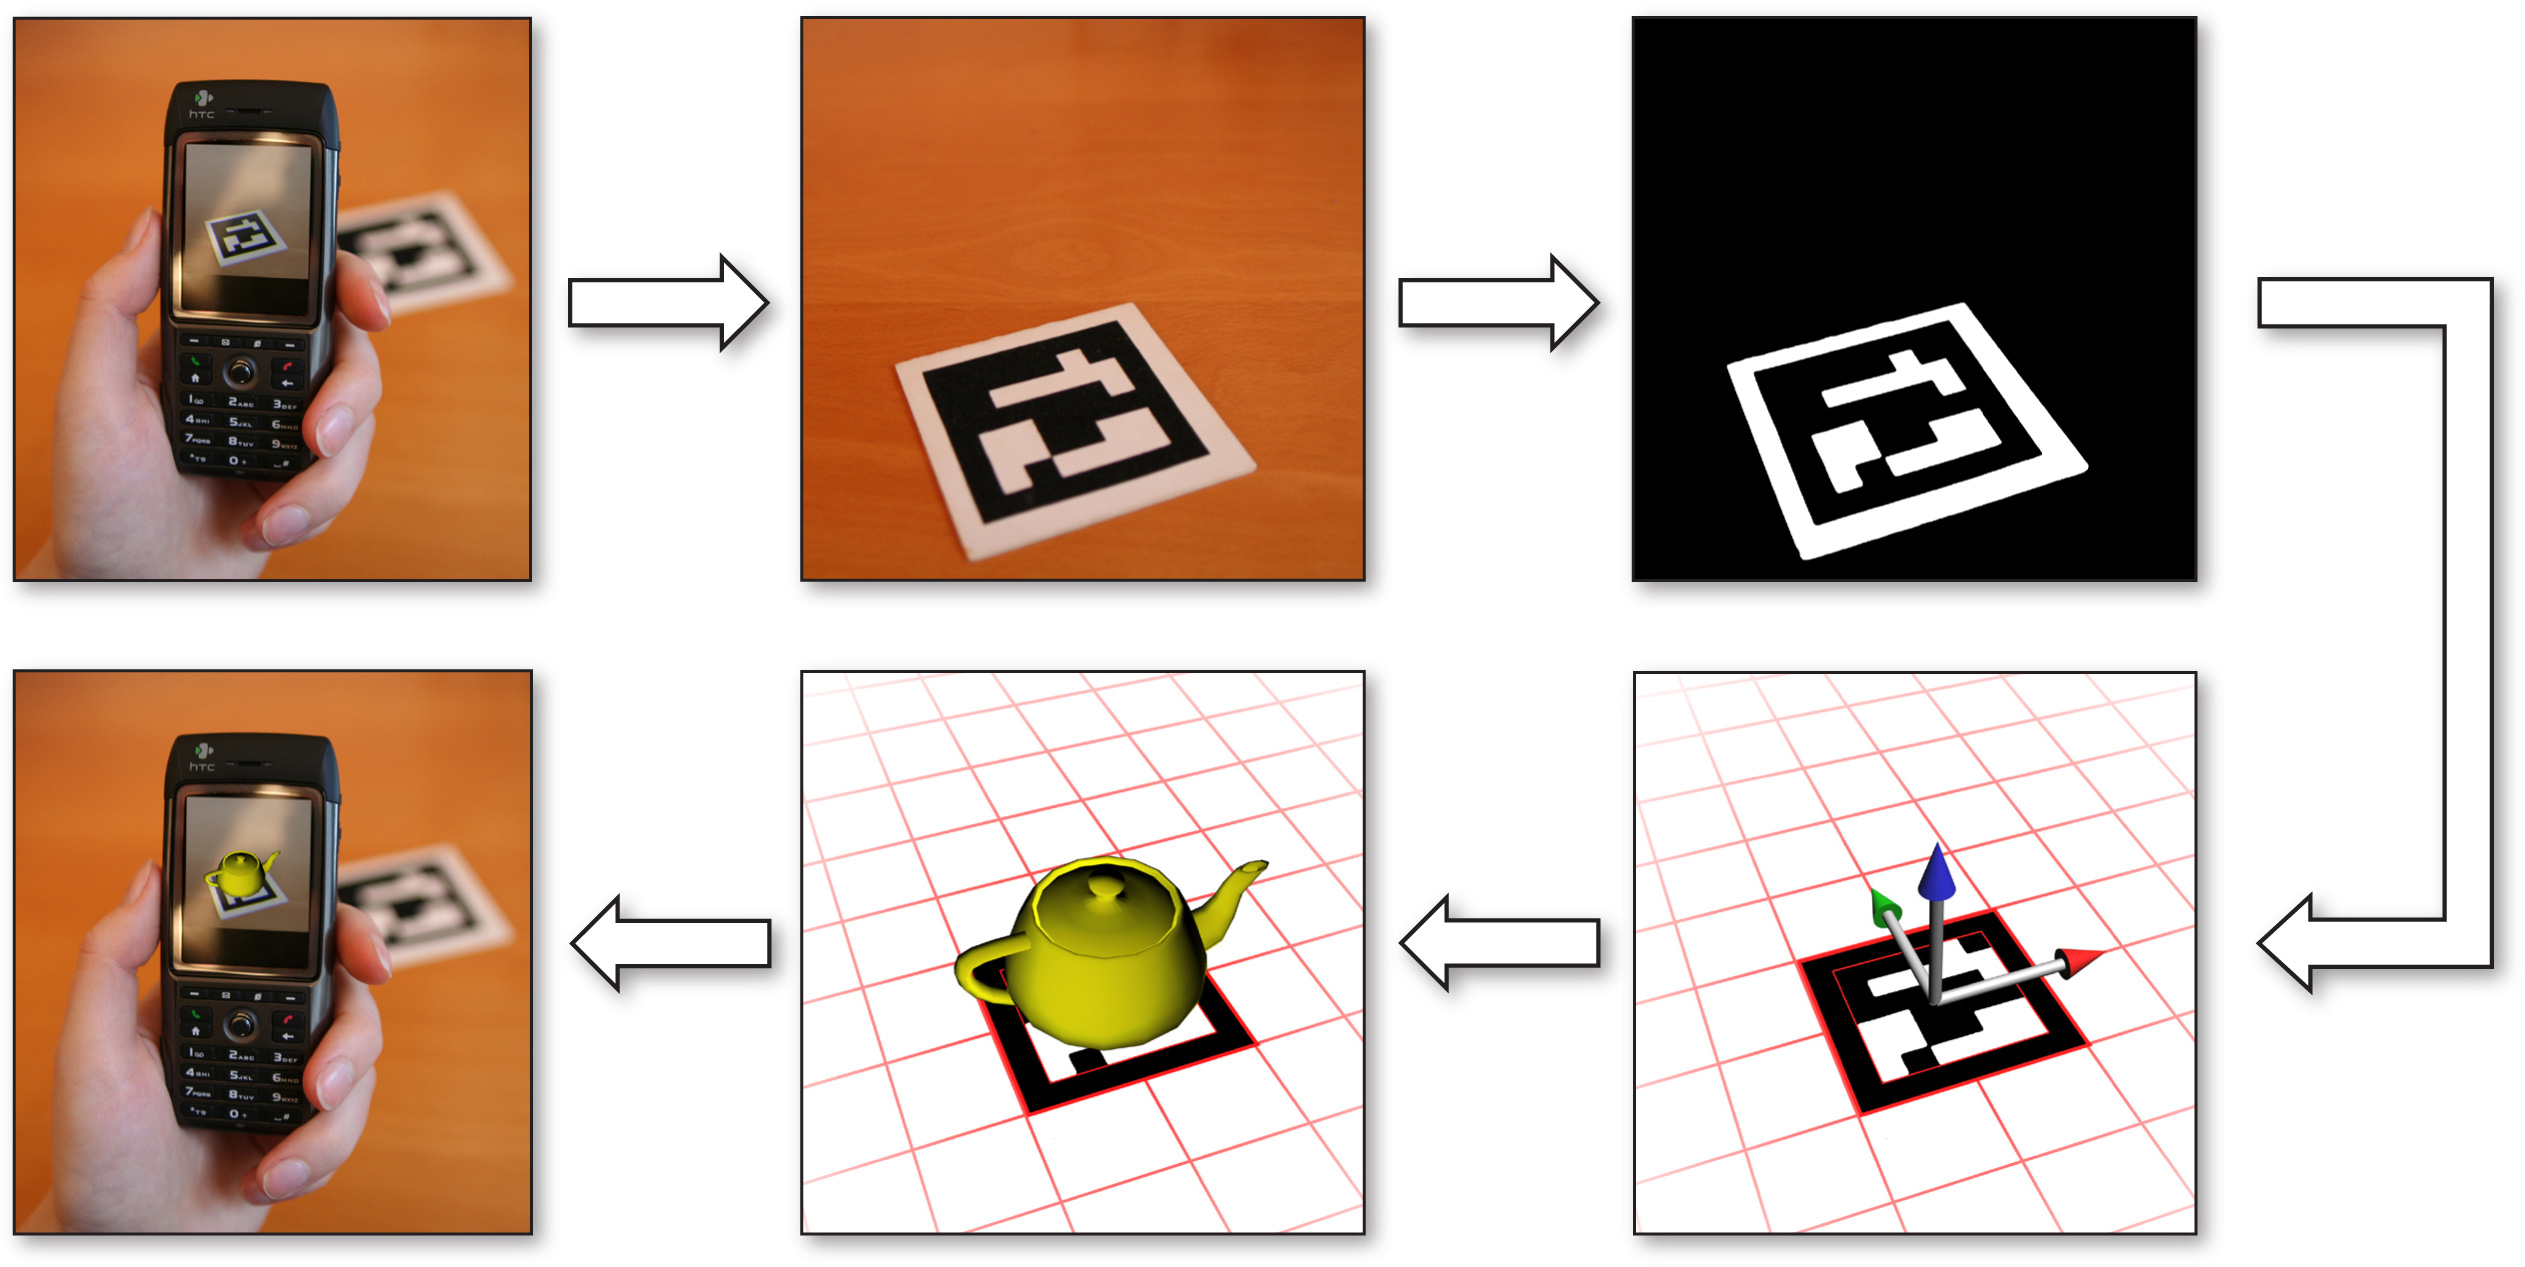
\includegraphics[scale=0.6, angle=0]{Files/Figures/HowMarkersWork.jpg}
    \caption[Παράδειγμα εντοπισμού marker και επαύξησης της σκηνής \cite{howmarkerswork}]{ Παράδειγμα εντοπισμού marker και επαύξησης της σκηνής \cite{howmarkerswork}}
    \label{fig:howmarkerswork}
\end{figure}


%siltanen
Ένας καλός marker πρέπει να μπορεί να ανιχνευθεί εύκολα και αξιόπιστα κάτω από όλες τις συνθήκες. Ορισμένες διαφορές στην φωτεινότητα(luminance) εντοπίζονται ευκολότερα από διαφορές στο χρώμα (colour) αν χρησιμοποιηθούν τεχνικές όρασης υπολογιστών \cite{hartley2003multiple} . Επιπλέον, ο φωτισμός αλλάζει τα αντιληφθέντα χρώματα των αντικειμένων και εποένως η ανίχνευση χρώματος είναι δύσκολη. Φυσικά, όσο περισσότερη αντίθεση φωτισμού υπάρχει, τόσο ευκολότερα εντοπίζονται αντικείμενα. Με αυτή την έννοια, η χρήση ασπρόμαυρων markers βελτιστοποιεί την διαδικασία ανίχνευσης. Το σύστημα πρέπει επίσης να μπορεί να υπολογίζει την πόζα της κάμερας με βάση το marker που εντοπίστηκε. Για να συμβεί αυτό, αρκεί να υπολογιστούν 4 σημεία και έτσι μπορούμε να υπολογίσουμε την μία και μοναδική λύση για την πόζα της κάμερας και ο ευκολότερος τρόπος για να συμβεί αυτό είναι η χρήση του σχήματος τετραγώνου για τα markers. Επιπλέον, οι θέσεις των γωνιακών σημείων είναι γενικά εύκολο να υπολογιστούν, καθώς αποτελούν ουσιαστικά την τομή των ακραίων ακμών ενός marker. Συμπερασματικά, τα περισσότερα συστήματα χρησιμοποιούν ασπρόμαυρους δείκτες και για αυτό το λόγο θα επεξηγηθεί στη συνέχεια η διαδικασία εντοπισμού ασπρόμαυρων markers.    


Ο πρωταρχικός στόχος, επομένως, μιας διαδικασίας ανίχνευσης marker είναι η εύρεση των περιγραμμάτων πιθανών markers και μετέπειτα η εξαγωγή των γωνιών τους στην εικόνα. Επιπλέον, το σύστημα ανίχνευσης πρέπει να εξακριβώσει ότι αυτό που βρέθηκε είναι όντως marker και να αποκωδικοποιήσει την ταυτότητα του. Τέλος το σύστημα υπολογίζει την πόζα, με βάση τις πληροφορίες από τη θέση στην οποία ανιχνεύθηκε ο marker.

Τα βασικά βήματα ανίχνευσης είναι τα παρακάτω:
\begin{itemize}


\item Image acquisition
Απόκτηση μίας εικόνας έντασης
δcquisition of an intensity image.
\item Preprocessing-Προεπεξεργασία
Επεξεργασία εικόνας σε χαμηλό επίπεδο-low level image processing
Αντιστροφή της Παραμόρφωσης(undistortion)
Ανίχνευση ακμών και προσαρμογή ακμών
Ανίχνευση γωνιών marker

Πριν από την πραγματική ανίχνευση ενός marker, το σύστημα πρέπει να πάρει μία εικόνας έντασης (greyscale image). Aν το format της εικόνας που καταγράφηκε είναι άλλου τύπου, πχ RGB, τότε θα μετασχηματιστεί σε εικόνας κλίμακας γκρι χρησιμοποιώντας μία γνωστές τεχνικές \cite{Gonzalez}. 
Πρώτος στόχος είναι η ανίχνευση των ορίων πιθανών markers. Συνήθως είτε γίνεται πρώτα κατωφλίωση της εικόνας και μετά αναζήτηση για markers από τη δυαδική εικόνα, ή γίνεται ανίχνευση ακμών από την εικόνα κλίμακας του γκρι. Αυτές οι μέθοδοι επεξεργασίας χαμηλού επιπέδου(thresholding,
edge detection, line fitting, etc.) είναι γνωστές και επομένως δε θα αναλυθούν περαιτέρω στη συγκεκριμένα εργασία. Ωστόσο οι αναγνώστες μπορούν να ανατρέξούν στα \cite{Gonzalez}, \cite{szeliski2010computer}, για περισσότερα παραδείγματα.

Τα συστήματα τα οποία χρησιμοποιούν προσεγγίσεις κατωφλίωσης, συνήθως χρησιμοποιούν μεθόδους προσαρμοστικής κατωφλίωσης (e.g. [75]) ώστε να αντιμετωπίσουν τις τοπικές αλλαγές φωτεινότητας. Μετά την κατωφλίωση το σύστημα έχει μία δυαδική εικόνα που αποτελείται από το παρασκήνιο και τα αντικείμενα. Όλα τα αντικείμενα είναι πιθανοί υποψήφιοι markers σε αυτό το στάδιο. Συνήθως η επόμενη φάση είναι η επισήμανσή τους ή η συνεχής ανίχνευση τους. Κατά τη διαδικασία επισήμανσης το σύστημα μπορεί να απορρίψει αντικείμενα τα οποία είτε είναι πολύ μικρά είτε είναι οτιδήποτε άλλο εκτός από marker. Τέλος οι ακμές όλων των πιθανών markers επισημαίνονται και οι θέσεις τους εξομαλύνονται(undistort) για το στάδιο του line fitting (Figure 26). Έπειτα, το σύστημα εξετάζει και πάλι πιθανά markers, ελέγχοντας αν έχουν 4 ευθείες γραμμές και 4 γωνίες. Τέλος, το σύστημα βελτιστοποιεί τις θέσεις των γωνιών με ακρίβει sub-pixel. Figure 27 δείχνει το σύστημα συντεταγμένων του marker και την μία επαύξηση ακριβώς από πάνω του.
Η ανίχνευση ακμών σε εικόνες κλίμακας του γκρι είναι μία διαδικασία που παίρνει αρκετό χρόνο και επομένως τα συστήματα συνήθως χρησιμοποιούν υποδειγματοληψία και ανιχνεύουν ακμές μόνο σε ένα προκαθορισμένο πλέγμα. Αυτή η προσέγγιση οδηγεί σε ξεχωριστά σημεία γραμμών, το σύστημα πρέπει να συνδέσει τα pixels των ακμών σε τμήματα, αξιοποιώντας την τεχνική edge sorting. As the system samples the
original points using a coarse grid, it needs to extend the lines to full length to find the exact corners of the marker. A common procedure is to use the gradient  information of the original image to extend the edges to full length.

Συνήθως οι εικόνες δεν είναι παραμορφωμένες, αφού χρησιμοποιείται η αντίστροφη διαδικασία παραμόρφωσης η οποία υπολογίστηκε κατά τη διαδικασία της βαθμονόμησης. Ωστόσο στα συστήματα πραγματικού χρόνου, εξομαλύνονται μόνο οι θέσεις των σημείων χαρακτηριστικών, π.χ οι ακμές ενός marker που ανιχνεύθηκαν για να επιταχυνθεί η διαδικασία. Η διαδικασία της βαθμονόμησης αναλύεται σε επόμενη ενότητα.

Ακόμα και μικρά λάθη σε εντοπισμένες δισδιάστατες θέσεις ακμών και γωνιών επηρεάζουν την πόζα της κάμερας όταν υπολογίζεται. [77–79]. Λάθη ανίχνευσης μπορεί να συμβούν λόγω σφάλματος κβαντοποίησης pixel, λαθασμένης τιμής ορίου κατωφλίωσης, θολώματος κίνησης, θορύβου κλπ. Αυτά τα σφάλματα προκαλούν ενοχλητικό τρέμουλο (jitter) στην πόζα ενός αντικειμένου, ακόμα και αν η κάμερα κινείται ελάχιστα. 
Για να βελτιωθεί η ακρίβεια, τα συστήματα βελτιστοποιούν τις θέσεις μετά την αρχική ανίχνευση.


\item Ανίχνευση πιθανών markers και απόρριψη προφανών non-markers 
Γρήγορη απόρριψη των προφανών non-markers
Γρήγορη αποδοχή των πιθανών markers.

Οι εφαρμογές επαυξημένης πραγματικότητας στοχεύουν σε επεξεργασία πραγματικού χρόνου και γρήγορες αποδόσεις καθώς αυτές θεωρούνται επιτακτικές. Τα συστήματα δεν μπορούν να αντέξουν χρόνο στην επεξεργασία στοιχείων που δεν είναι markers. 
Επομένως, πολλές υλοποιήσεις χρησιμοποιούν κριτήρια αποδοχής / απόρριψης για να ξεχωρίσουν τα πραγματικά markers από τα αντικείμενα που προφανώς είναι κάτι άλλο.

Στη συνέχεια αναλύουμε ορισμένα τέτοια τεστ που χρησιμοποιούνται συχνά.
Ένα σύστημα μπορεί να απορρίψει περιοχές που αποτελούνται μόνο από μερικά pixels. Συνήθως οι περιοχές αυτές δεν είναι markers, αλλά και να ήταν, το μικρό μέγεθός τους θα σήμαινε ότι το marker είναι πολύ μακριά από την κάμερα. Σε αυτή την περίπτωση η πόζα του marker δε θα ήταν πολύ ακριβής και απομένως άχρηστη. Επιπλέον, αν το marker συρρικνωθεί σε μέγεθος μερικών μόνο pixels, το σύστημα δε θα μπορεί να το αναγνωρίσει, εκτός αν κρατά ιστορικό εμφάνισης κάθε marker.
Το σύστημα πρέπει να δίνει προσοχή σε περιοχές στο εσωτερικό των markers και να σιγουρευτεί ότι δεν αφαιρεί κομμάτια ή στοιχεία που ανήκουν στο marker. Το ιστόγραμμα ενός ασπρόμαυρου marker είναι διπολικό και το σύστημα μπορεί να αξιοποιήσει τη διπολικότητα αυτή ως ένα κριτήριο για γρήγορη αποδοχή ή απόρριψη. Ωστόσο, το τεστ πρέπει να λάβει υπόψη του τις αντανακλάσεις που μπορεί να δημιουργήσουν τιμές στη μέση του ιστογράμματος (γκρι). Ο υπολογισμός του αριθμού των εικονοστοιχείων που ανήκουν στην περίμετρο είναι μία γρήγορη διαδικασία η οποία μπορεί να πραγματοποιηθεί στο στάδιο της επισήμανσης, σε αντίθεση με τον υπολογισμό του μεγέθους του αντικειμένου που είναι πιο περίπλοκο και απαιτεί χρόνο. Ένα άλλο γρήγορο κριτήριο που χρησιμοποιείται για την εκτίμηση της περιοχής, είναι η μέγιστη διαγώνιος ή άνοιγμα. Μερικές φορές ένα σύστημα μπορεί να απορρίψει περιοχές που είναι πολύ μεγάλες αν έχει γνώση για να δικαιολογήσει το συμπέρασμα ότι είναι κάτι άλλο εκτός από marker, πχ σκοτεινές ακμές λόγω vignetting.

Το βέλτιστο όριο για το μέγεθος ενός marker εξαρτάται από την εφαρμογή και τον τύπο του marker.
Για παράδειγμα, το ARToolKit συμπεραίνει ότι τα markers είναι σε μία λογική απόσταση από την κάμερα. Η ανίχνευση markers του ARToolKit παραβλέπει περιοχές που είναι πολύ μεγάλες ή πολύ μικρές μετά την επισήμανση. Με άλλα λόγια, κρατά τις περιοχές όπου ο αριθός των pixels που ανήκουν σε αυτές είναι μέσα στα όρια για περαιτέρω ανάλυση.
Ανάλογα με τον τύπο του marker, ένα σύστημα μπορεί να γνωρίζει κάτι για την συνολική εμφάνιση του marker. Για παράδειγμα, τα απλά πρότυπα markers έχουν μία μαύρη εκόνα σε μία λευκή περιοχή που περιβάλλεται από μία μαύρη ακμή.
Σε μία ιδεατή περίπτωση, οι markers έχουν ένα γνωστό αριθμό από τρύπες (λευκές περιοχές) μέσα σε μία μαύρη περιοχή του marker. Επιπλέον οι περιοχές που είναι εντελώς μαύερες, δεν είναι markers σίγουρα.Ο υπολογισμός του αριθμού των τρυπών είναι γρήγορος και επομένως ένα σύστημα μπορεί να εφαρμόσει σαν κριτήριο απόρριψης τον αριθμό των οπών, κατά την προεπεξεργασία. Για παάδειγμα, το maerker στα αριστερά της εικόνα 28 έχεια μία λευκή οπή μέσα στο μαύρο όριο και το marker στη μέση έχει 3 οπές. Τα δυαδικά markers 2D barcode (π.χ το marker δεξιά στην εικόνα 28) έχουν ένα αριθμό δυνατών ακμών μέσα στο marker. 

Μια ευρετική μέθοδος απόρριψης προφανών μη-markers είναι ο υπολογισμός αριθμού αλλαγών έντασης σε δύο κάθετες κατευθύνσεις. Αν ο αριθμός αλλαγών είναι χαμηλός, τότε δεν μπορεί να είναι marker. Αυτό το κριτήριο λειτουργεί μόνο σε τύπους markers όπου η κωδικοποίηση εγγυάται υψηλή διακύμανση και μη ύπαρξη σχεδόν λευκών ή σχεδόν μαύρων markers. 
Μία προοπτική εικόνα ενός τετραφώνου είναι πάντα τετράπλευρη. Επομένως, βολεύει να εφαρμοστεί ένα τεστ τετραπλεύρων για τετράγωνα markers. Ο αριθμός γραμμών και γωνιών είναι εύκολο να υπολογίστει και επομένως οι υλοποιήσεις ανίχνευσης markers χρησιμοποιούν το συγκεκριμένο κριτήριο.
Για παράδειγμα το ARToolKit χρησιμοποιεί line fitting για τα pixels των ακμών για να ελέγξει την ύπαρξη ακριβώς 4 γραμμών στην περίμετρο [83]. 

Οι υπολογιστικά φθηνοί αλγόριθμοι συνήθως χρησιμοποιούν ορισμένες ευρετικές μεθόδους, όπως την εύρεση 4 γωνιών με χρήση απλών αλγορίθμων μέγιστων αποστάσεων (maximum diagonal) όπως στα [84] and [85]. Επιπροσθέτως, αυτές οι γωνίες μπορούν να χρησιμοποιηθούν ως αρχικές εκτιμήσεις για ανίχνευση γωνιών Harris. Σαν αποτέλεσμα το σύστημα χρειάζεται να εξομαλύνει μόνο τα 4 εντοπισμένα γωνιακά σημεία. 

Επιπλέον, το σύστημα μπορεί να εφαρμόσει και άλλα γρήγορα κριτήρια, ανάλογα με τον τύπο των markers, πχ για κυκλικά markers, ένα κριτήριο εξαρτάται από κάποιο τέστ κυκλικότητας. Στην επεξεργασία πραγματικού χρόνου, το σύστημα πρέπει να επικεντρώνεται στην επεξεργασία σχετικών πληροφοριών και επομένως αυτά τα γρήγορα τεστ είναι ιδιαίτερα σημαντικά. Τα τεστ αυτά πραγματοποιούνται από τα συστήματα καθόλη τη διάρκεια της ανίχνευσης markers και της διαδικασίας ταυτοποίησης. 

\item Identification and decoding of markers
Ταίριασμα template 
Αποκωδικοποίηση data marker
\item Υπολογισμός πόζας marker
Εκτίμηση της πόζας marker
Επαναληπτικός υπολογισμός πόζας για εύρεση ακριβούς πόζας

Το στάδιο της απόκτησης εικόνας είναι ουσιαστικά μια ξεχωριστή διαδικασία. Παρέχει την εικόνα για να ξεκινήσει η διαδικασία ανίχνευσης.

Γενικά οι διαδικασίες ανίχνευσης marker μπορούν να διαφέρουν από την παραπάνω σειρά βημάτων. Μπορεί η σειρά εκτέλεσης να είναι διαφορετική ή το σύστημα να συνενώσει βήματα στον ίδιο αλγόριθμο. Συγκεκριμένα, πολλές υλοποιήσεις συνδυάζουν τεστ αποδοχής/απόρριψης με άλλες διεργασίες. Το σύστημα μπορεί να απορρίψει ένα υποψήφιο marker σε οποιοδήποτε στάδιο της ανίχνευσης, μόλις παρατηρήσει ότι ο υποψήφιος δεν μπορεί να είναι marker. Ωστόσο η βασική αρχή είναι η ίδια συνήθως. 

\end{itemize}
%---



Η διαδικασία εντοπισμού ενός marker περιλαμβάνει τη χρήση αλγορίθμων για τη κατωφλίωση της εικόνας και την εύρεση ακμών χρησιμοποιώντας μία scanline αναζήτηση.  Γνωρίζοντας τις ακμές του markers, μπορούμε να βρούμε το ορθογώνιο εκείνο το οποίο ταιριάζει στο marker, αντιστοιχίζοντας τις γωνίες με βάση τις μέγιστες διαγωνίους ανάμεσα στα σημεία των ακμών. Αυτό γίνεται με στόχο την οριοθέτηση ενός ορθογωνίου παραλληλογράμου ώστε να αναγνωριστεί ένα πρότυπο κι να αντιστοιχιστεί με βάση τα πρότυπα που είναι αποθηκευμένα στη μνήμη. Μόλις αναγνωριστεί το πρότυπο αυτό, υπολογίζεται η πόζα του markers, εκτιμώντας τις παραμέτρους περιστροφής και μετατόπισης σε σχέση με την κάμερα. Αυτό γίνεται χρησιμοποιώντας ένα πίνακα μετασχηματισμού (transformation matrix) που διαμορφώνεται με τα διανύσματα γωνιών και μετατόπισης (rotation \& translation vectors). Με άλλα λόγια, ψάχνουμε να βρούμε τις συντεταγμένες του markers ως προς τις συντεταγμένες της κάμερας, χρησιμοποιώντας τα σημεία μετασχηματισμού τα οποία ονομάζονται εξωτερικές παράμετροι (extrinsic parameters) και αλλάζουν ανάλογα με την κίνηση της κάμερας και τις εσωτερικές παραμέτρους που χρησιμοποιούνται για να μετακινηθούμε από τις συντεταγμένες τις κάμερας στις συντεταγμένες της εικόνα και είναι ορισμένες εκ των προτέρων ανάλογα με την κάμερα και τις παραμέτρους που υπολογίζονται κατά τη βαθμονόμησή της, δηλαδή την εστιακή απόσταση, τις παραμέτρους κλίμακας και τις συντεταγμένες του της εικόνας προβολής.

Αφού έχει εντοπιστεί η θέση του marker, ένα εικονικό μοντέλο τοποθετείται στην ίδια θέση της των συντεταγμένων της εικόνας σε σχέση με το δείκτη. Αυτό δίνει στο χρήστη την εντύπωση ότι το εικονικό αντικείμενο είναι κολλημένο πάνω στο δείκτη και η διαδικασία αυτή ονομάζεται registration. Η τελική εικόνα απεικονίζεται στην οθόνη, όπου ο χρήστης βλέπει το εικονικό αντικείμενο πάνω από την πραγματική σκηνή. Η διαδικασία πραγματοποιείται δυναμικά και αρκετά γρήγορα, ώστε να δίνεται η αίσθηση ότι της αλληλοσυσχέτισης πραγματικού και εικονικού κόσμου. Δεν είναι υπολογιστικά ακριβή διαδικασία, αλλά το marker πρέπει να αναγνωρίζεται εύκολα, π.χ οι συνθήκες φωτιμού πρέπει να είναι ευνοϊκές και δεν πρέπει να γίνεται επικάλυψη του marker, π.χ από τα χέρια του χρήστη, διότι τότε θα αποτύχει η διαδικασία της ανίχνευσης. 


Στην διπλωματική αυτή εργασία, χρησιμοποιήθηκε η βιβλιοθήκη επαυξημένης πραγματικότητας ArUco. Η διαδικασία που χρησιμοποιείται για την ανίχνευση ενός marker κρίνεται σκόπιμο να αναλυθεί στη συνέχεια.

%aruco


\begin{itemize}
\item Εφαρμογή προσαρμοστικής κατωφλίωσης για την λήψη ορίων σχημάτων (Figure 1)

\begin{figure}[H]
    \centering
    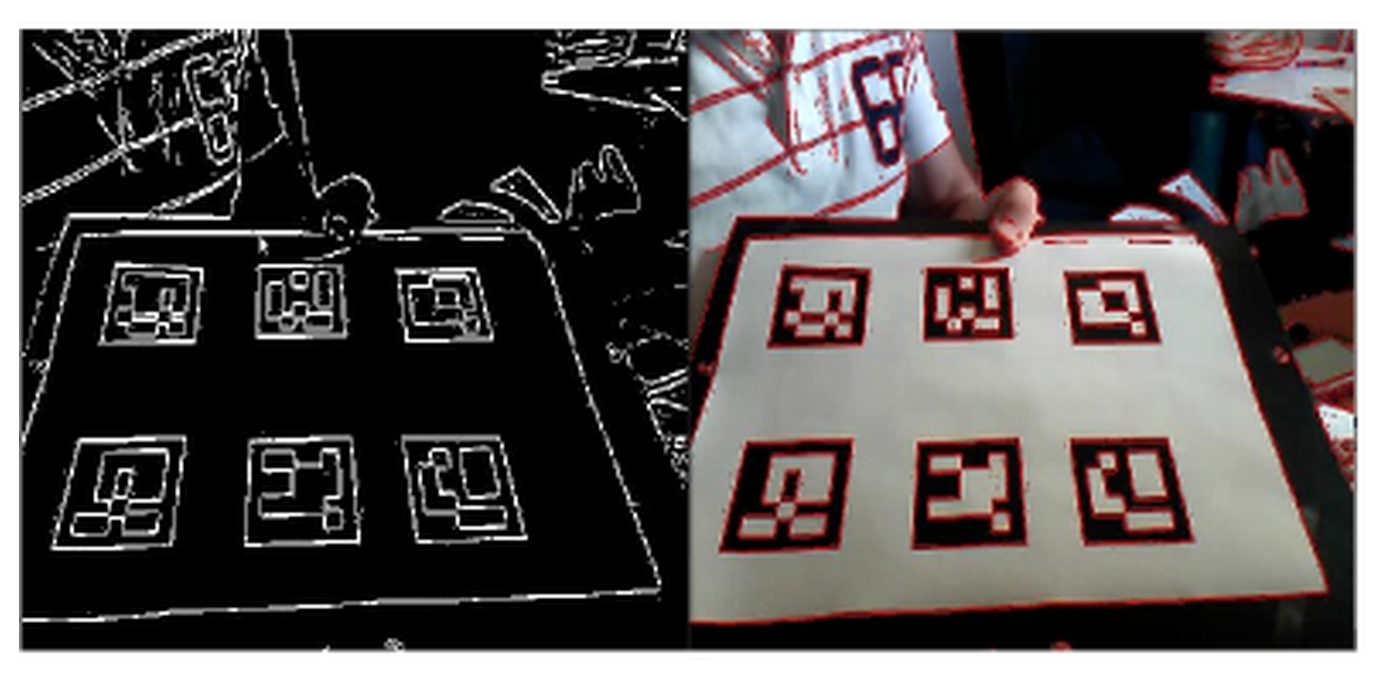
\includegraphics[scale=0.6, angle=0]{Files/Figures/aruco1.png}
    \caption[Παράδειγμα εντοπισμού marker και επαύξησης της σκηνής \cite{howmarkerswork}]{ Παράδειγμα εντοπισμού marker και επαύξησης της σκηνής }
    \label{fig:aruco1}
\end{figure}


\item Εύρεση περιγραμμάτων. Μόλις γίνει αυτό, ανιχνεύονται όχι μόνο τα πραγματικά markers, αλλά και πολλά όρια σχημάτων που δε χρειάζονται.Η υπόλοιπη διαδικασία στοχεύει στο φιλτράρισμα των ορίων που δεν χρειάζονται.
\begin{itemize}
\item Αφαίρεση συνόρων με ένα μικρό αριθμό σημείων(Figure 2)


\begin{figure}[H]
    \centering
    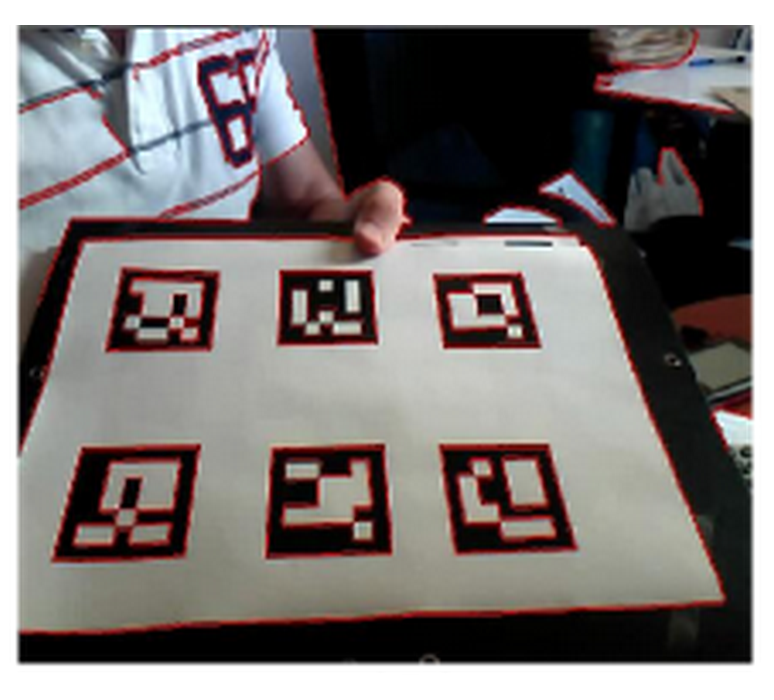
\includegraphics[scale=0.6, angle=0]{Files/Figures/aruco2.png}
    \caption[Παράδειγμα εντοπισμού marker και επαύξησης της σκηνής \cite{howmarkerswork}]{ Παράδειγμα εντοπισμού marker και επαύξησης της σκηνής \cite{howmarkerswork}}
    \label{fig:aruco2}
\end{figure}



\item Πολυγωνική προσέγγιση των περιγραμμάτων και διατήρηση των κοίλων περιγραμμάτων με 4 γωνίες (π.χ τετραγώνων) (Figure 3)



\begin{figure}[H]
    \centering
    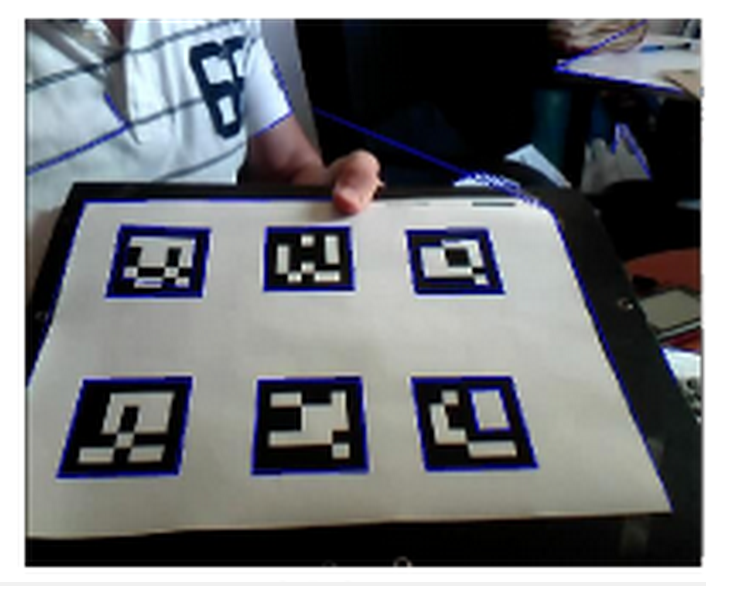
\includegraphics[scale=0.6, angle=0]{Files/Figures/aruco3.png}
    \caption[Παράδειγμα εντοπισμού marker και επαύξησης της σκηνής \cite{howmarkerswork}]{ Παράδειγμα εντοπισμού marker και επαύξησης της σκηνής \cite{howmarkerswork}}
    \label{fig:aruco3}
\end{figure}


\end{itemize}
\item Ταξινόμηση των γωνιών με φορά ανίθετης της κατεύθυνσης του ρολογιού.
\item Αφαίρεση πολύ κοντινών ορθογωνίων. Αυτό απαιτείται διότι η προσαρμοστική κατωφλίωση συνήθως ανιχνεύει το εξωτερικό μέρος του ορίου ενός marker. Σε αυτό το στάδιο κρατάμε το περισσότερο εξωτερικό σύνορο. (Figure 4)


\begin{figure}[H]
    \centering
    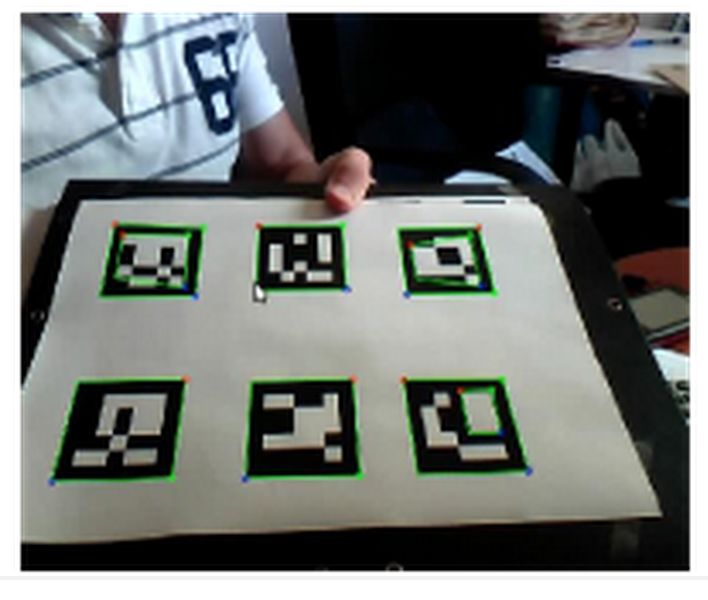
\includegraphics[scale=0.6, angle=0]{Files/Figures/aruco4.png}
    \caption[Παράδειγμα εντοπισμού marker και επαύξησης της σκηνής \cite{howmarkerswork}]{ Παράδειγμα εντοπισμού marker και επαύξησης της σκηνής \cite{howmarkerswork}}
    \label{fig:aruco4}
\end{figure}


\item Ταυτοποίηση Marker (Marker Identification)
\begin{itemize}
\item Αφαίρεση της προοπτικής προβολής ώστε να πάρουμε μία εμπροσθια όψη της τετραγωνικής περιοχής χρησιμοποιώντας τις αρχές της ομογραφίας (homography). (Figure 5)


\begin{figure}[H]
    \centering
    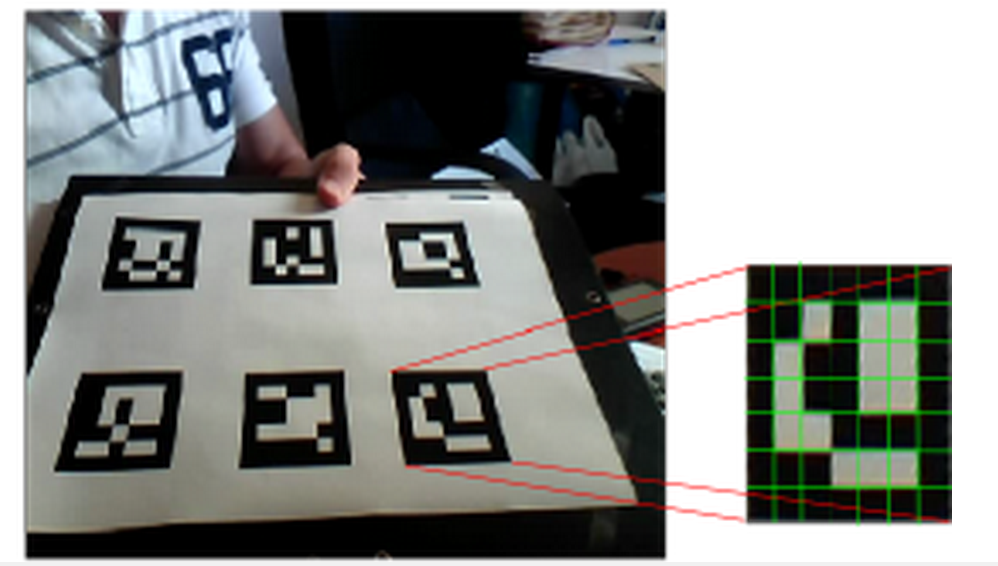
\includegraphics[scale=0.6, angle=0]{Files/Figures/aruco5.png}
    \caption[Παράδειγμα εντοπισμού marker και επαύξησης της σκηνής \cite{howmarkerswork}]{ Παράδειγμα εντοπισμού marker και επαύξησης της σκηνής \cite{howmarkerswork}}
    \label{fig:aruco5}
\end{figure}


\item Κατωφλίωση της εικόνας χρησιμοποιώντας τη μέθοδο Otsu.Η μέθοδος αυτή είναι μια μη παραμετρική μέθοδος κατωφλίωσης η οποία βασίζεται στο ιστόγραμμα της εικόνας. Πιο συγκεκριμένα βρίσκει εκείνο το κατώτατο όριο το οποίο ελαχιστοποιεί τη διακύμανση κάθε κλάσης των οριοθετημένων μαύρων και άσπρων pixels. Με άλλα λόγια η προσέγγιση αυτή επιλέγει το κατώφλι το οποίο έχει ως αποτέλεσμα την πιο σφιχτή ομαδοποίηση των δύο ομάδων που αναπαρίστανται από τα pixels παρασκηνίου και προσκηνίου. 
\item Ταυτοποίηση του εσωτερικού κωδικού. Το marker υποδιαιρείται σε ένα πλέγμα 6x6, όπου τα εσωτερικά 5x5 κελιά περιέχουν την πληροφορία για το ID του marker. Τα υπόλοιπα αντιστοιχούν σε ένα εξωτεριό μαύρο σύνορο. Η βιβλιοθήκη της ArUco ελέγχει πρώτα αν το εξωτερικό μαύρο σύνορο υπάρχει. Έπειτα, διαβάζουμε τα εσωτερικά 5x5 κελιά και ελέγχουμε αν παρέχουν έναν έγκυρο κωδικό(ίσως χρειαστεί η περιστροφή του κωδικού για να πάρουμε έγκυρο κωδικό). 



\begin{figure}[H]
    \centering
    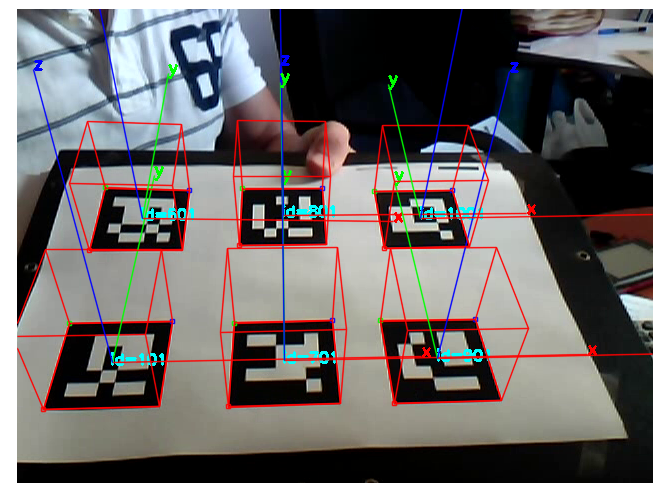
\includegraphics[scale=0.6, angle=0]{Files/Figures/aruco6.png}
    \caption[Παράδειγμα εντοπισμού marker και επαύξησης της σκηνής \cite{howmarkerswork}]{ Παράδειγμα εντοπισμού marker και επαύξησης της σκηνής \cite{howmarkerswork}}
    \label{fig:aruco5}
\end{figure}


\end{itemize}
\item Για τα έγκυρα markers, βελτιώνουμε τις γωνίες χρησιμοποιώντας subpixel  παρεμβολή.
\item Τέλος, αν δίνονται οι παράμετροι της κάμερας, υπολογίζεται η σχετική θέση του marker ως προς την κάμερα.
\end{itemize}








\subsection{Το Μοντέλο Κάμερας Pinhole}


%gt pinhole?
Στα πεδία της υπολογιστικής όρασης και των γραφικών, το απλούστερο μαθηματικό μοντέλο, το οποίο περιγράφει τη σχέση μεταξύ των συντεταγμένων χώρου ενός αντικειμένου και της προβολής τους στην εικόνα είναι το μοντέλο κεντρικής προβολής. Στην πραγματικότητα, η κεντρική προβολή περιγράφει με ακρίβεια μόνο τη μηχανή σημειακής οπής (pinhole camera), με αποτέλεσμα να αναφέρεται συχνά και ως pinhole camera model \cite{hartley2003multiple} .


Το μοντέλο αυτό, βασίζεται στην θεώρηση ότι όλες οι ακτίνες φωτός περνούν μέσα από μία οπή αμελητέων διαστάσεων και το είδωλο ενός αντικειμένου προβάλλεται πάνω στο επίπεδο μιας εικόνας. Επειδή μέσω της κεντρικής προβολής δημιουργούνται ανεστραμμένες εικόνες \cite{fig:pinhole3}, πολλές φορές καθίσταται βολική η θεώρηση του επιπέδου προβολής μπροστά από την μικροσκοπική οπή, στην ίδια απόσταση που βρισκόταν και προηγουμένως, με αποτέλεσμα η φανταστική αυτή εικόνα να μην είναι ανεστραμμένη. 



\begin{figure}[H]
    \centering
    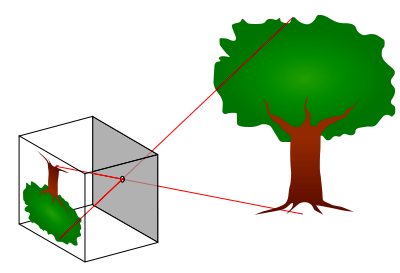
\includegraphics[scale=0.5, angle=0]{Files/Figures/pinhole3.png}
    \caption[Το μοντέλο κεντρικής προβολής (pinhole camera model)]{ Το μοντέλο κεντρικής προβολής (pinhole camera model) \cite{pinhole} .}
    \label{fig:pinhole3}
\end{figure}

%εδω ξεκιναμε να λέμε για τα focal length kai ideal to sensor 
Στις ψηφιακές κάμερες, η εικόνα εγγράφεται στον αισθητήρα της εικόνας και οι συντεταγμένες των στοιχείων του διαφέρουν από τις ιδανικές συντεταγμένες. Η εικόνα της κάμερας εξαρτάται από τα φυσικά χαρακτηριστικά της κάμερας, όπως την εστιακή απόσταση, τον προσανατολισμό του αισθητήρα και το μέγεθος. H εικόνα, λοιπόν, η οποία δεν αποτελεί μία αυστηρά κεντρική προβολή, λόγω ποικίλων σφαλμάτων που οφείλονται στους φακούς, στην ατμόσφαιρα, κ.λπ., προσεγγίζεται γεωμετρικά από το μοντέλο αυτό, στο πλαίσιο της όρασης υπολογιστών.

Το σχήμα~\ref{fig:pinhole2} δείχνει το μοντέλο κάμερας pinhole. 



%περιγραφη της εικονας γεωμετρικα

\begin{figure}[H]
    \centering
    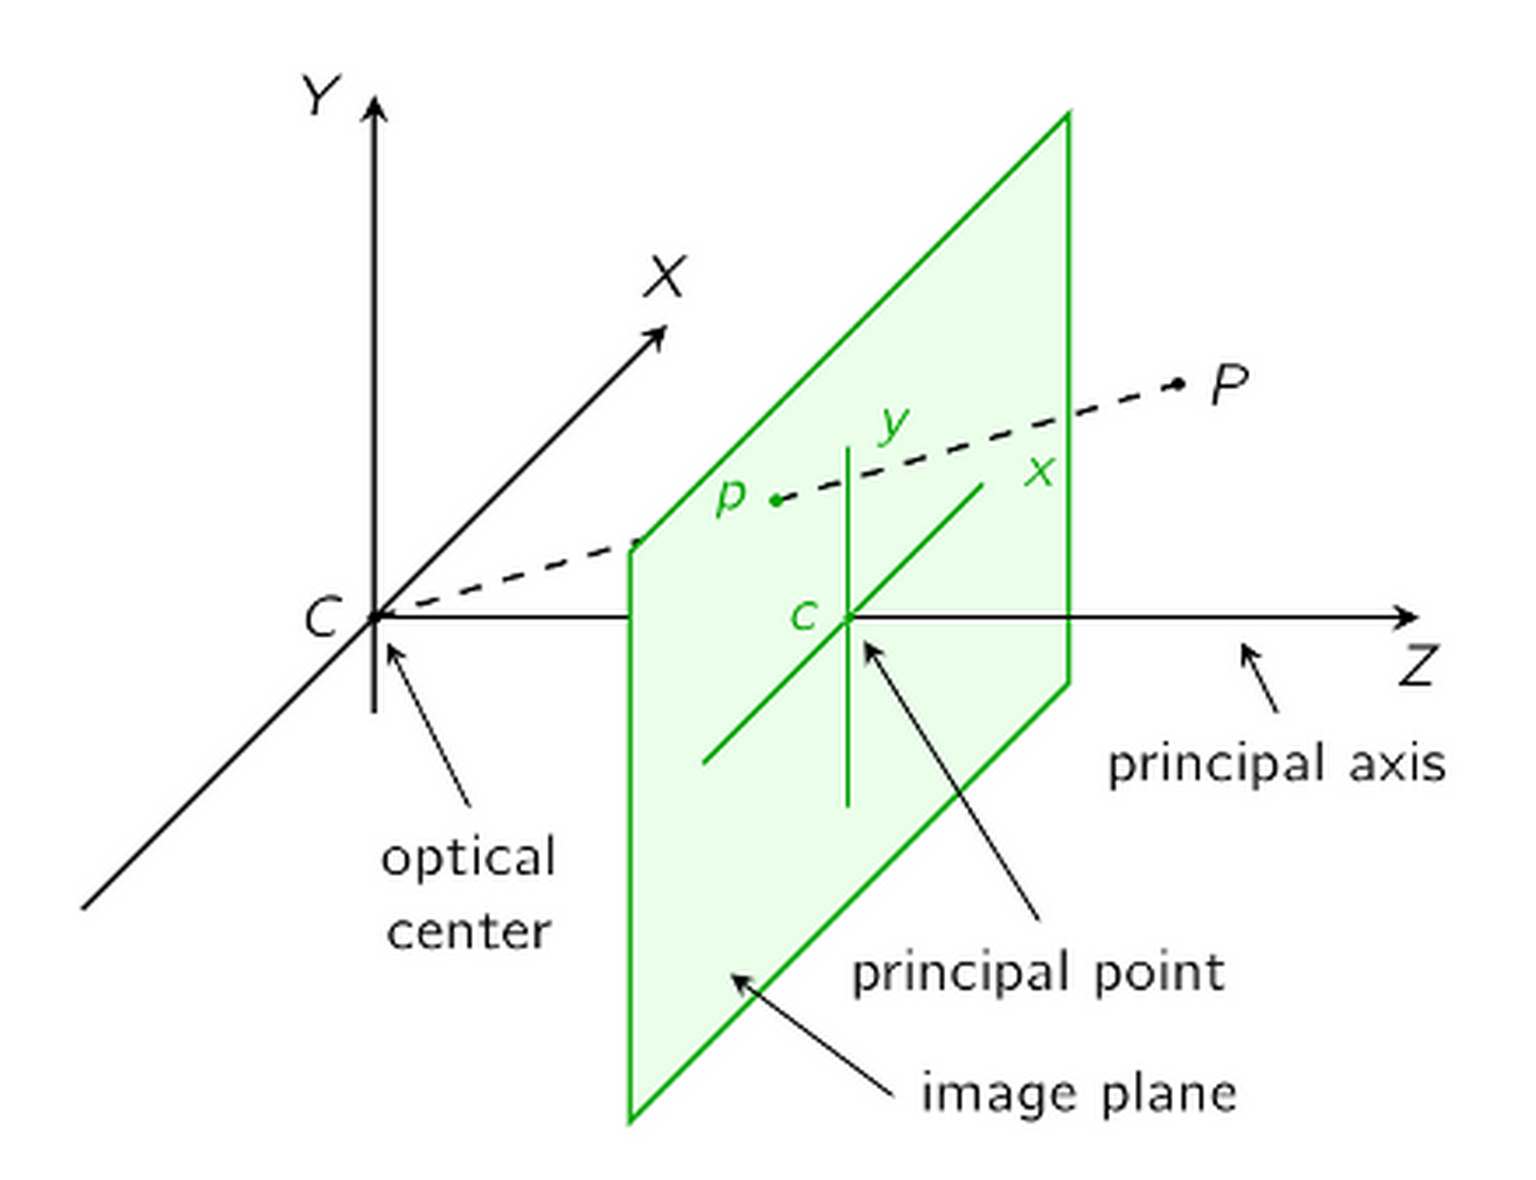
\includegraphics[scale=0.5, angle=0]{Files/Figures/pinhole1.png}
    \caption[Το μοντέλο κεντρικής προβολής στις 3 διαστάσεις (pinhole camera model)]{ Το μοντέλο κεντρικής προβολής (pinhole camera model) \cite{pinhole} .}
    \label{fig:pinhole1}
\end{figure}


\begin{figure}[H]
    \centering
    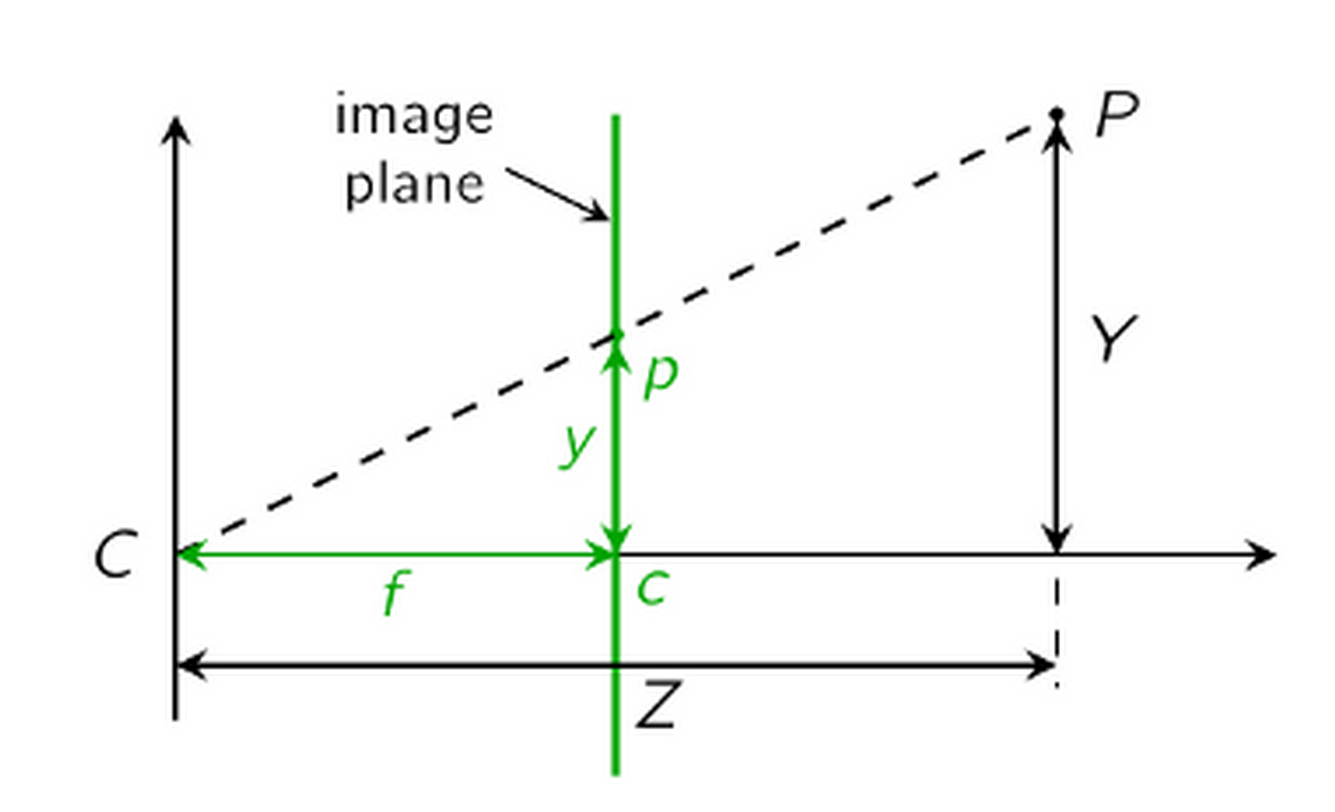
\includegraphics[scale=0.5, angle=0]{Files/Figures/pinhole2.png}
    \caption[Πλάγια όψη του μοντέλου κεντρικής προβολής 2D (pinhole camera model)]{ Πλάγια όψη του μοντέλου κεντρικής προβολής (pinhole camera model) \cite{pinhole} .}
    \label{fig:pinhole2}
\end{figure}

To principal point είναι η τομή ανάμεσα στο principal axis και το επίπεδο της εικόνας. Το optical center είναι το σημείο pinhole, το οποίο παίζει κεντρικό ρόλο στην όλη διαδικασία. Η εικόνα μιας pinhole κάμερας σχηματίζεται στο επίπεδο $Z=f$, όπου f είναι το εστιακό μήκος κάμερας(focal length).

Το μοντέλο κάμερας pin-hole χρησιμοποιείται συχνά στην υπολογιστική όραση και τα γραφικά υπολογιστών για την μοντελοποίηση της προβολικής μετρατοπής μίας τρισδιάστατης σκηνής σε ένα δισδιάστατο επίπεδο προβολής \cite{hartley2003multiple} .
Το επίπεδο αυτό, που περνάει από το principal point και είναι παράλληλο στο επίπεδο της εικόνα ονομάζεται image plane.

Ό άξονας που ξεκινά από το optical center και το principal point και διαπερνά κάθετα το image plane ονομάζεται principal axis.








Συμπεραίνοντας ότι έχουμε οποιοδήποτε άλλο σημείο P = [X, Y, Z] στο 3Δ χώρο, και αν θεωρήσουμε το επίπεδο της εικόνας για να ορίσουμε τη δισδιάστατη εικόνα, τότε η δισδιάστατη προβολή του P σχηματίζεται στο σημείο τομής ανάμεσα στο επίπεδο της εικόνας και της γραμμής που σχηματίζεται ανάμεσα στο κέντρο της εστίασης και το P, που ορίζεται ως p = [x, y]. 



%ksekinoun mathematics
Το μοντέλο της κάμερας έχει στόχο να μετασχηματίσει ένα οποιδήποτε 3D σημείο $X = \begin{bmatrix} X & Y & Z \end{bmatrix}$ σε ένα 2D σημείο $X = \begin{bmatrix} x & y\end{bmatrix}$. 




Για να συμβεί αυτό, αρκεί μία απλή προοπτική προβολή. Χρησιμοποιώντας τη μέθοδο όμοιων τριγώνων στο σχήμα~\ref{pinhole2} παίρνουμε τις παρακάτω σχέσεις:


\begin{equation}
\begin{aligned}
X=f\frac{X}{Z}\\
Y=f\frac{Y}{Z}
\end{aligned}
\end{equation}


Η μεταβλητή $f$ συμβολίζει το εστιακό μήκος, ενώ ε μορφή ομογενών συντεταγμένων, η παραπάνω σχέση γράφεται ως:

\begin{equation}
\begin{bmatrix}
x\\y\\1
\end{bmatrix}
=
\begin{bmatrix}
f & 0 & 0 & 0\\
0 & f & 0 & 0\\
0 & 0 & 1 & 0
\end{bmatrix}
\begin{bmatrix}
X\\
Y\\
Z\\
1
\end{bmatrix}
\end{equation}



Ο παραπάνω πίνακας ονομάζεται και camera projection matrix.


%ideal != sensor image 2d

Ωστόσο θεωρήθηκε ότι το σύστημα συντεταγμένων του image plane έχει την αρχή των αξόνων του στο principal point, κάτι που δεν ισχύει απαραίτητα πάντα. Έτσι πρέπει να τροποιηθεί το παραπάνω μοντέλο ώστε να ληφθεί υπόψη αυτή η μετατόπιση του συστήματος συντεταγμένων.



\begin{equation}
x=f\frac{X}{Z}+c_{x} \! \!  y=f\frac{Y}{Z}+c_{y}
\end{equation}

όπου $(c_{x},c_{y})^{T}$ είναι οι συντεταγμένες του principal point, δηλαδή του σημείου στο οποίο, ο οπτικός άξονας τέμνει το επίπεδο της εικόνας. 

Οπότε και πάλι σε ομογενείς συντεταγμένες έχουμε:

\begin{equation}
\begin{bmatrix}
x\\y\\1
\end{bmatrix}
=
\begin{bmatrix}
f & 0 & c_{x} & 0\\
0 & f & c_{y} & 0\\
0 & 0 & 1 & 0
\end{bmatrix}
\begin{bmatrix}
X\\
Y\\
Z\\
1
\end{bmatrix}
\end{equation}

Ένας τρόπος που χρησιμοποιείται, συνήθως, είναι η αναπαράσταση του μοντέλου της κάμερας ως ένας πίνακας βαθμονόμησης κάμερας (intrinsic camera calibration matrix) K, ή απλά πίνακας κάμερας (camera matrix).  Έχουμε, λοιπόν, τον πίνακα intrinsic camera calibration matrix, Κ, ο οποίος γράφεται ως:


\begin{equation}
K=
\begin{bmatrix}
f & 0 & c_{x}\\
0 & f & c_{y}\\
0 & 0 & 1
\end{bmatrix}
\end{equation}



Το μοντέλο αυτό, υποθέτει ότι οι συντεταγμένες εικόνας είναι ευκλείδειες συντεταγμένες που έχουν ίδιες κλίμακες και στις 2 κατευθύνσεις των αξόνων, δηλαδή ότι έχουμε τετράγωνα pixels. Αν ωστόσο δε συμβαίνει κάτι τέτοιο, τότε ο μετασχηματισμός από κοσμικές συντεταγμένες σε συντεταγμένες pixel βρίσκεται πολλαπλασιάζοντας την προηγούμενη εξίσωση με το διάνυσμα $\begin{bmatrix}m_{x} & m_{y} & 1\end{bmatrix}$. Οπότε έχουμε τον πίνακα K ο οποίος παίρνει τη μορφή:

\begin{equation}
K=
\begin{bmatrix}
a_{x} & 0 & c_{x}\\
0 & a_{y} & c_{y}\\
0 & 0 & 1
\end{bmatrix}
\end{equation}

όπου $a_{x}=fm_{x}$ και $a_{y}=fm_{y}$ είναι το εστιακό μήκος κάμερας σε όρους διαστάσεων pixels στις κατευθύνσεις x και y αντίστοιχα. Ωστόσο συνήθως στις περισσότερες κάμερες $m_{x}=m_{y}$.

Μερικές φορές ο πίνακας αυτός παίρνει τη μορφή:

\begin{equation}
K=
\begin{bmatrix}
a_{x} & s & c_{x}\\
0 & a_{y} & c_{y}\\
0 & 0 & 1
\end{bmatrix}
\end{equation}

για μεγαλύτερη γενικότητα, όπου $s$ είναι μία παράμετρος λοξότητας (skew) των στοιχείων pixels, η οποία ορίζεται ως η γωνία των δύο πλευρών του κάθε pixel του αισθητήρα και θεωρεί ότι τα pixels δεν είναι πάντα ορθογώνια, αλλά μπορεί να είναι απλά παραλληλόγραμμα. Ωστόσο, με το σημερινό επίπεδο κατασκευής των αισθητήρων, μπορούμε να θεωρήσουμε με ασφάλεια, ότι η παράμετρος αυτή είναι 0, δηλαδή ότι τα pixels του αισθητήρα είναι ορθογώνια.
Σήμερα ωστόσο οι αισθητήρες μπορεί να θεωρηθεί ότι έχουν τα pixels τους αισθητήρα ορθογώνια, επομένως το s είναι συνήθως μηδενικό. 





Εποένως, τα φυσικά χαρακτηριστικά μιας κάμερας είναι εκείνα που ορίζουν πώς θα διαμορφωθεί μία εικόνα στον αισθητήρα εικόνας μιας κάμερας. 








\begin{figure}[H]
    \centering
    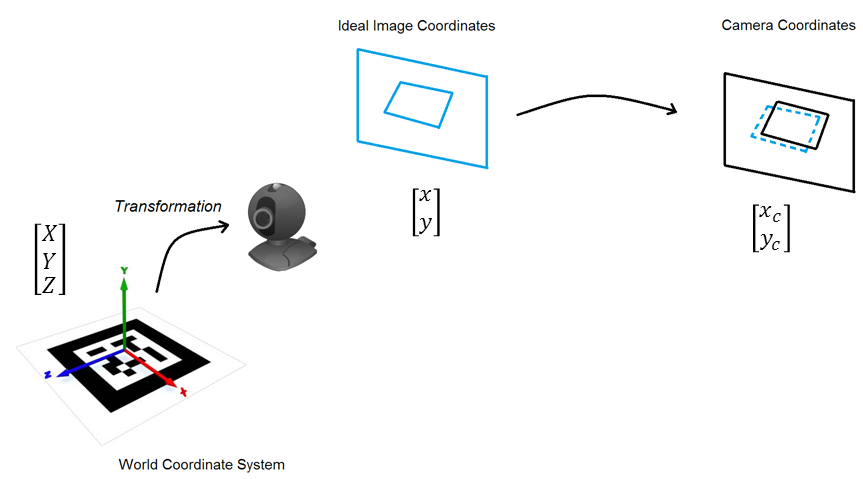
\includegraphics[scale=0.6, angle=0]{Files/Figures/transformation1.png}
    \caption[Στιγμιότυπο κατά τη διαδικασία της βαθμονόμησης κάμερας μέσω της OpenCV]{ Στιγμιότυπο κατά τη διαδικασία της βαθμονόμησης κάμερας μέσω της OpenCV}
    \label{fig:transformation1}
\end{figure}








%------------DISTORTIONS---------------------------------------

Mία πραγματική κάμερα μπορεί να παράγει συστηματικά γεωμετρικά σφάλματα, που ονομάζονται παραμορφώσεις, λόγω ατελειών του φακού. 
Επομένως, θεωρητικά, η παραμόρφωση πρέπει να ληφθεί υπόψη πριν γίνει ο μετασχηματισμός των ιδανικών συντεταγμένων σε συντεταγμένες κάμερας. 



Σε αυτή την περίπτωση, η παραμόρφωση μπορεί να μοντελοποιηθεί μετά μετά τον εσωτερικό μετασχηματισμό της κάμερας (camera’s intrinsic transformation). Ο πίνακας κάμερας μετατρέπει τις ιδανικές συντεταγμένες εικόνας σε συντεταγμένες κάμερας και έπειτα, η συνάρτηση παραμόρφωσης μετατρέπει τις συντεταγμένες κάμερας σε συντεταγμένες pixel.

\begin{equation}
D
\left(
\begin{bmatrix}
x_{c}\\
y_{c}   
\end{bmatrix}
\right )
=
\begin{bmatrix}
x_{pix}\\
y_{pix}   
\end{bmatrix}
\end{equation} 


\begin{equation}
D^{-1}
\left (
\begin{bmatrix}
x\\
y  
\end{bmatrix}
\right )
)=
\begin{bmatrix}
x_{c}\\
y_{c}
\end{bmatrix}
\end{equation} 


Η αντίστροφη συνάρτηση παραμόρφωσης $D^{-1}$, εξομαλύνει τις συντεταγμένες pixel σε συντεταγμένες κάμερας.




Συνοπτικά, ένα σύστημα εντοπισμού marker μπορεί να μετατρέψει τις συντεταγμένες εικόνας που παρατηρεί (pixel coordinates) μιας βαθμονομημένης κάμερας σε συντεταγμένες ιδανικής οθόνης. 


Οι συντεταγμένες pixel μετασχηματίζονται πρώτα σε συντεταγμένες κάμερας και μετά εξομαλύνονται:

\begin{equation}
K^{-1}D^{-1} 
\left (\begin{bmatrix}
x_{pix}\\ 
y_{pix}
\end{bmatrix}  \right )
=K_Α{-1}
\left (\begin{bmatrix}
x_{c}\\ 
y_{c}
\end{bmatrix}  \right )
=
\begin{bmatrix}
x\\ 
y
\end{bmatrix}
\end{equation}

Από την άλλη πλευρά, οι ιδανικές συντεταγμένες μπορούν να μετασχηματιστούν σε κοσμικές συντεταγμένες και αντίστροφα. Τέλος, μπορούμε να αναπαραστήσουμε τη σχέση ανάμεσα σε στις κοσμικές συντεταγμένες $X$ και τις παρατηρούμενες συντεταγμένες εικόνας $x_{pix}$,

\begin{equation}
K^{-1}D^{-1} 
\left (\begin{bmatrix}
x_{pix}\\ 
y_{pix}
\end{bmatrix}  \right )
=D
\left (KT \begin{bmatrix}
X\\ 
Y\\
Z
\end{bmatrix}  \right )
\end{equation}


Συνήθως η ακτινική παραμόρφωση μπορεί να αγνοηθεί, εκτός κι αν κρίνεται απαραίτητη η υψηλή ακρίβεια σε όλα τα μέρη της εικόνας. 



%------------END DISTORTIONS---------------------------------------





\subsection{Παράμετροι Κάμερας}

Για να πάρουμε το συγκεκριμένο πίνακα προβολής, για μία αυθαίρετη θέση της κάμερας στο χώρο, πρέπει να υπολογιστούν ανεξάρτητα οι εσωτερικές και οι εξωτερικές παράμετροι της κάμερας. 


Υπάρχουν δύο υποσύνολα παραμέτρων κάμερας που μπορούν να χρησιμοποιηθούν προκειμένου να καθοριστεί η σχέση ανάμεσα στα συστήματα συντεταγμένων.
Γνωστά ως εσωτερικές και εξωτερικές παράμετροι στο πεδίο της όρασης υπολογιστών, ορίζονται ως:



-Intrinsics-
Οι εσωτερικές παράμετροι είναι αυτές που σχετίζονται με την εσωτερική γεωμετρία μίας κάμερας και ορίζουν την αντιστοίχιση των συντεταγμένων στο σύστημα συντεταγμένων της εικόνας (2D) και στο σύστημα συντεταγμένων της κάμερας \cite{Malik2002}. Με άλλα λόγια αναπαριστούν τα οπτικά, γεωμετρικά και ψηφιακα χαρακτηριστικά μιας κάμερας και είναι :

\begin{itemize}
\item Το εστιακό μήκος
\item Η θέση του principal point στο pixel space
\item Ο συντελεστής s σχετικά με το σχήμα των pixels του αισθητήρα
\item οι συντελεστές παραμόρφωσης του φακού
\end{itemize}




-Extrinsics-

%extrinsics
Οι παραπάνω διαδικασίες υπολογισμού των εσωτερικών παραμέτρων της κάμερας υποθέτουν ότι γνωρίζουμε την 3Δ θέση ενός σημείου ως προς το σύστημα συντεταγμένων της κάμερας. Αν θέλουμε να βρούμε την προβολή του σημείου το οποίο ορίζεται ως προς ένα αυθαίρετο σύστημα συντεταγμένων, τότε πρέπει να βρούμε τις εξωτερικές παραμέτρους που ορίζουν το μετασχηματισμό. Οι εξωτερικές παράμετροι(extrinsics) ορίζουν τη θέση και το προσανατολισμό της κάμερας ( ή ακριβέστερα του συστήματος συντεταγμένων της κάμερας σε σχέση με τις κοσμικές συντεταγμένες της σκηνής). 

Έχουμε επομένως 2 συστήματα συντεταγμένων:

\begin{itemize}
\item Το σύστημα συντεταγμένων της κάμερας 
\item Το σύστημα συντεταγμένων του κόσμου (world coordinates system-WCS)
\end{itemize}


Ένα σημείο μπορεί να εκφραστεί με την κατάλληλη μορφή σε οποιοδήποτε από αυτά τα 2 συστήματα συντεταγμένων

Έτσι εαν:

\begin{itemize}
\item $\tilde{X}$ το ομογενές διάνυσμα ενός σημείου σε κοσμικές συντεταγμένες
\item $\tilde{X_{cam}}$ το ομογενές διάνυσμα του ίδιου σημείου στο σύστημα συντεταγμένων της κάμερας
\item $\tilde{C}$ οι συντεταγμένες του κέντρου της κάμερας στο WCS
\item R ο πίνακας 3x3 Rotation
\end{itemize}

Έχουμε:

\begin{equation}
\tilde{X_{cam}}=R(\tilde{X}-\tilde{C})
\end{equation}

Ενώ αν θέσουμε 


\begin{equation}
t=-R\tilde{C}
\end{equation}


Έχουμε 

\begin{equation}
\tilde{X_{cam}}=R\tilde{X}+t
\end{equation}


και ο πίνακας προβολής είναι

\begin{equation}
P=K [R \! | \!t]
\end{equation}





ή σε ομογενείς συντεταγμένες :

\begin{equation}
\begin{bmatrix}
x \\ y \\ z
\end{bmatrix}
=
\begin{bmatrix}
r_{1} & r_{2} & r_{3} & t_{x}\\
r_{4} & r_{5} & r_{6} & t_{y}\\
r_{7} & r_{8} & r_{9} & t_{z}
\end{bmatrix}
\begin{bmatrix}
X\\
Y\\
Z\\
1
\end{bmatrix}
\end{equation}

Όπως είναι γνωστό, ένας πίνακας περιστροφής έχει μόνο τρεις παραμέτρους $(\alpha, \beta, \gamma)$ οι οποίες ορίζουν τα 9 στοιχεία του. Ένα διάνυσμα μετατόπισης έχει επίσης 3 παραμέτρους και επομένως ο πίνακας πόζας έχει 6 ελεύθερες παραμέτρους. Όπως μπορεί να γίνει εύκολα αντιληπτό, ο συνδυασμός αυτός της rotation και της translation μπορεί να μοντελοποιήσει οποιαδήποτε κίνηση της κάμερας. Ένα σύστημα εντοπισμού marker πρέπει να λύνει αυτό τον πίνακα (camera matrix) σε κάθε frame, όταν ανιχνεύει έναν marker.






\subsection{Βαθμονόμηση Κάμερας}
%Η ΔΙΑΔΙΚΑΣΙΑ ΒΑΘΜΟΝΟΜΗΣΗΣ ΚΑΙ ΓΕΝΙΚΑ Η ΘΕΩΡΙΑ ΑΠΟ ΠΙΣΩ(ΤΟ ΠΩς ΓΙΝΕΤΑΙ ΣΤΟ ΚΕΦΑΛΑΙΟ 4)


Η διαδικασία της βαθμονόμησης περιλαμβάνει, ουσιαστικά, την ταυτοποίηση των εσωτερικών παραμέτρων της κάμερας, δηλαδή του πίνακα κάμερας και την εκτίμηση της συνάρτησης παραμόρφωσης.


Οι εφαρμογές επαυξημένης πραγματικότητας συχνά χρησιμοποιούν ξεχωριστά εργαλεία βαθμονόμησης ή διενεργούν την διαδικασία βαθμονόμησης ξεχωριστά από την εφαρμογή. Συνήθως το εργαλείο βαθμονόμησης αποθηκεύει τα αποτελέσματα σε ένα αρχείο, το οποίο διαβάζει η εφαρμογή επαυξημένης πραγματικότητας. Από εδώ και στο εξής θα θεωρούμε ότι η συνάρτηση εξομάλυνσης (undistortion) $D^{-1}$ αι ο πίνακας βαθμονόμησης Κ είναι γνωστά. 


%clarke
Η εύρεση των εσωτερικών παραμέτρων της κάμερας είναι γνωστή ως βαθμονόμηση κάμερας ή camera calibration και στόχο έχει τον προσδιορισμό των στοιχείων του εσωτερικού προσανατολισμού της κάμερας από δισδιάστατες εικόνες. Αυτές περιλαμβάνουν την εστιακή απόσταση, το "principal point" και την αναλογία των διαστάσεων (aspect ratio). 

Η συνολική απόδοση μιας εφαρμογής επαυξημένης πραγματικότητας, εξαρτάται άμεσα από την ακρίβεια της βαθμονόμησης της κάμερας. Παρά το γεγονός ότι το αντικείμενο παρουσιάζει ιδιαίτερο ερευνητικό ενδιαφέρον, δεν είναι στους στόχους της εργασίας η περαιτέρω ανάλυσή του. Στα πλαίσια της διπλωματικής εργασίας απαιτείται η χρήση μιας απλής μεθόδου με αξιοποίηση συνηθισμένου εξοπλισμού για την βαθμονόμηση. 


%σκακιερα
Καταφεύγουμε λοιπόν, στη λύση του εργαλείου της Opencv για την βαθμονόμηση της κάμερας[80], που προσφέρει μία έτοιμη και αποτελεσματική λύση, με χρήση μίας απλής κάμερας και μιας απλής επίπεδης εικόνας και συγκεκριμένα του μοτίβου τετραγώνων σκακιέρας, η οποία χρειάζεται απλά να εκτυπωθεί σε απλό χαρτί. 
Γενικά, η βαθμονόμηση μέσω της καταγραφής πολλαπλών λήψεων ενός επίπεδου αντικειμένου με χαρακτηριστικά σημεία, όπως είναι η σκακιέρα, επιτυγχάνεται με δεδομένα τις συντεταγμένες χώρου και εικόνας των αντίστοιχων σημείων, οι πρώτες εκ των οποίων προκύπτουν αυτόματα, ενώ οι τελευταίες αναγνωρίζονται στην εικόνα ομοίως με αυτόματο τρόπο. Ωστόσο, για την εξασφάλιση σωστών αποτελεσμάτων από τη διαδικασία της βαθμονόμησης, οι εικόνες του αντικειμένου πρέπει να ληφθούν από διαφορετικά σημεία και υπό διαφορετικές γωνίες. 




Αυτό το οποίο θα πρέπει να συγκρατήσει ο αναγνώστης, είναι ότι μέσω της διαδικασίας της βαθμονόμησης παίρνουμε τις εσωτερικές παραμέτρους της κάμερας μέσω μιας offline διαδικασίας που πραγματοποιείται μόνο μία φορά στην αρχή της διαδικασίας ανάπτυξης της εφαρμογής. Οι παράμετροι που υπολογίζονται, ορίζονται ως είσοδος στην εφαρμογή που θα αναπτυχθεί, προκειμένου να λειτουργήσει σωστά. Επομένως, δε χρειάζεται να πραγματοποιείται βαθμονόμηση κάθε φορά πριν ξεκινήσει μία εφαρμογή επαυξημένης πραγματικότητας. Αρκεί να γίνει μόνο μία φορά στην αρχή, εκτός και αν τα αποτελέσματα δεν έχουν αρκετή ακρίβεια. Ωστόσο αν σε ένα σύστημα επαυξημένης πραγματικότητας χρησιμοποιηθεί διαφορετική κάμερα, τότε πρέπει να γίνει εκ νέου βαθμονόμηση για τη νέα κάμερα.












\subsection{Εκτίμηση Θέσης Marker}

%-SUNDUASMOS EXTRINSIC-INTRINSIC APO CAMERA PARAMETERS PDF

%malik
-συστήματα συντεταγμένων
Οι παρακάτω 3 μετασχηματισμοί όπως περιγράφονται στο \cite{Vallino1998}, που πρέπει να γίνουν γνωστοί πριν την ανάπτυξη εφαρμογών επαυξημένης πραγματικότητας είναι οι μετασχηματισμοί αντικειμένου-σε-κοσμικές, κοσμικές-σε-κάμερας, κάμερας-σε-επίπεδο εικόνας. 

\textbf{Object-to-World Transformations ($M_{O}$)}

Αν υποθέσουμε ότι έχουμε ένα εικονικό αντικείμενο κεντραρισμένο ως προς το τοπικό του σύστημα συντεταγμένων, το $M_{O}$ ορίζεται ως ο μετασχηματισμός από το τοπικό αυτό σύστημα σε μία θέση και έναν προσανατολισμό μέσα στο κοσμικό σύστημα συντεταγμένων που ορίζει την κύρια σκηνή.

\textbf{World-to-camera ($M_{c}$)}

Ο μετασχηματισμός $M_{c}$ ορίζει τη θέση και τον προσανατολισμό (πόζα) της βιντεοκάμερας που χρησιμοποιείται για τη θέαση της κύριας σκηνής, επιτρέποντας σε σημεία του πραγματικού κόσμου να οριστούν ως προς την κάμερα.

\textbf{Camera-to-image plane ($M_{p}$)}

Ο μετασχηματισμός $M_{p}$ ορίζει μία προβολής από το 3D χώρο στο 3D χώρο, έτσι ώστε οι συντεταγμένες της κάμερας να μπορούν να μετασχηματιστούν σε συντεταγμένες εικόνας, προκειμένου να μπορούν να προβληθούν σε μία οθόνη ή σε ένα HMD.


\begin{figure}[H]
    \centering
    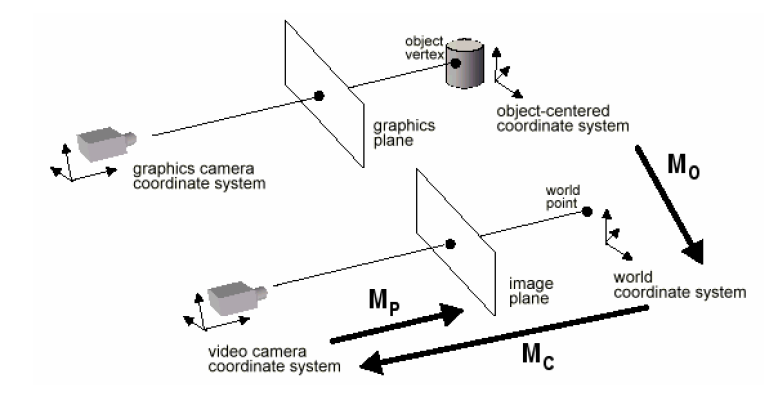
\includegraphics[scale=1.3, angle=0]{Files/Figures/coordinatesystems.png}
    \caption[Συστήματα Συντεταγμένων στην Επαυξημένη Πραγματικότητα]{Συστήματα Συντεταγμένων στην Επαυξημένη Πραγματικότητα}
    \label{fig:coordinatesystems}
\end{figure}

Για να μπορέσει μία εφαρμογή επαυξημένης πραγματικότητας να απεικονίσει σωστά ένα εικονικό τρισδιάστατο αντικείμενο πάνω από μία πραγματική σκηνή, οι παραπάνω γεωμετρικοί μετασχηματισμοί πρέπει να είναι ακριβείς.

H σημασία τους στην επαυξημένη πραγματικότητα είναι τεράστια.
Ένα σφάλμα σε οποιαδήποτε από τις σχέσεις θα κάνει ανακριβές το registration, ελαττώνοντας το ρεαλισμό της τελικής επαυξημένης σκηνής. 

Χρησιμοποιώντας ομογενή συστήματα συντεταγμένων, η προφανής ενός τρισδιάστατου σημείου στον Ευκλείδιο χώρο [x, y, z, w] χρησιμοποιώντας την παρακάτω εξίσωση:

\begin{equation}
\begin{bmatrix}
u & v & h
\end{bmatrix}
^{T}=
M_{P(3x4)}M_{C(4x4)}M_{O(4x4)}
\begin{bmatrix}
x & y & z & w
\end{bmatrix}
^{T}
\end{equation}






Η εύρεση των εξωτερικών παραμέτρων ( με δεδομένη την εκ των προτέρων γνώση των εσωτερικών παραμέτρων) δίνει τη θέση και τον προσανατολισμό της κάμερας σε σχέση με τον πραγματικό δισδιάστατο κόσμο είναι γνωστή σαν εκτίμηση πόζας (pose estimation).




\begin{figure}[H]
    \centering
    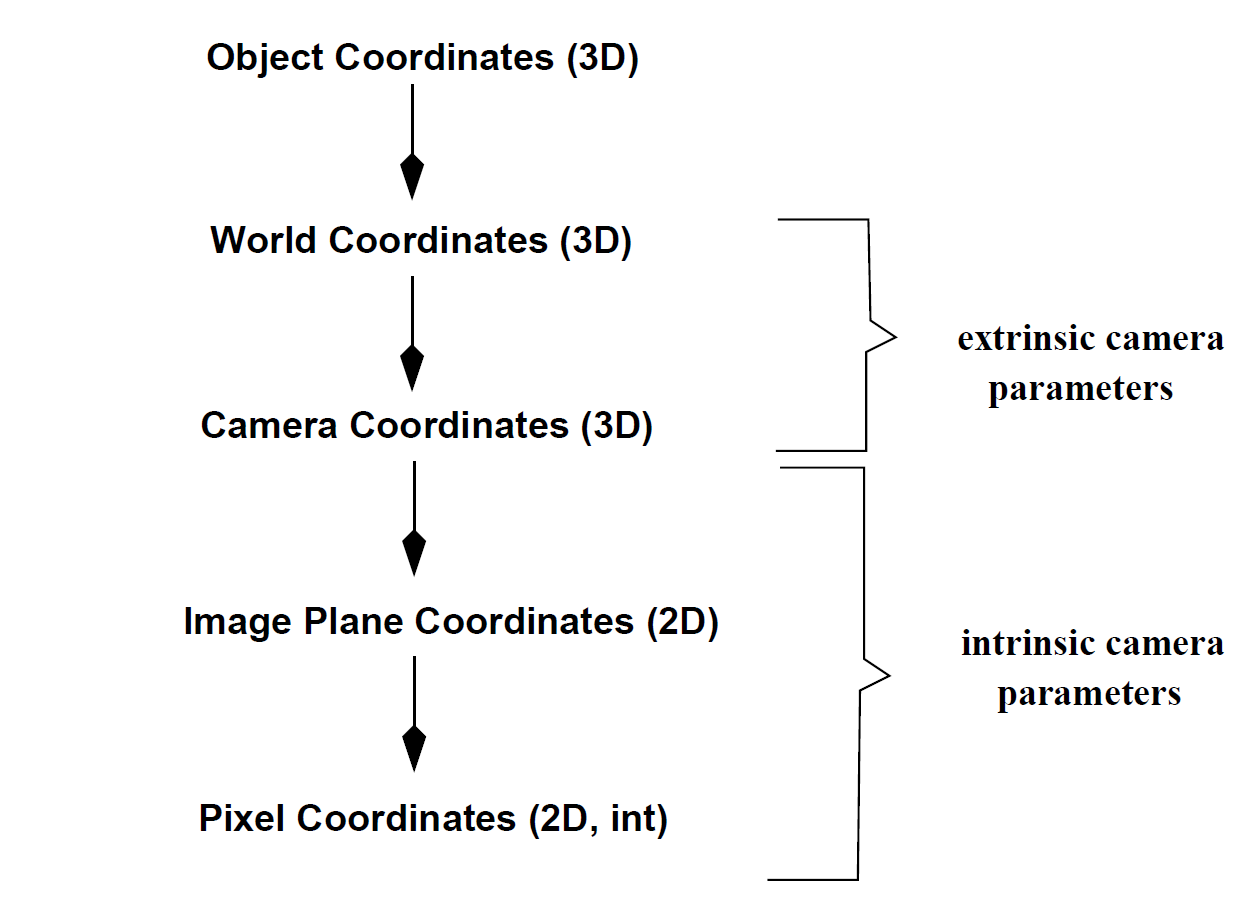
\includegraphics[scale=0.7, angle=0]{Files/Figures/coordinatesDiagram.png}
    \caption[Σειρά μετασχηματισμών]{ Σειρά μετασχηματισμών}
    \label{fig:coordinatesDiagram}
\end{figure}



\subsection{Multimarker Setup}




%from summary
Στις προηγούμενες ενότητες αναφερθήκαμε στις διαδικασίες, εκείνες, που είναι απαραίτητες για την ανίχνευση markers σε μία σκηνή με στόχο την εύρεση της σχετικής θέσης της κάμερας ως προς το marker. Ωστόσο ο εντοπισμός ενός marker μπορεί να αποτύχει για διάφορους λόγους όπως οι κακές συνθήκες φωτισμού της σκηνής, ορισμένες γρήγορες κινήσεις της κάμερας, αποκρύψεις του marker από άλλα αντικείμενα ή από τα χέρια του χρήστη κ.λ.π. 



Για να λυθεί αυτό το πρόβλημα, ορισμένες βιβλιοθήκες επιτρέπουν τη χρήση πολλαπλών markers μαζί τα οποία ονομάζονται πεδία markers ή markerboards. Ένα markerboard είναι ένας markers που αποτελείται από αρκετούς άλλους markers καθορισμένους σε μία διάταξη. Τα markerboards παρουσιάζουν δύο κύρια πλεονεκτήματα. 

Πρώτα απ'όλα έχουν περισσότερα από ένα markers, που σημαίνει ότι είναι δυσκολότερο να χαθούν όλα την ίδια στιμή. Επίσης όσο περισσότερα markers ανιχνευθούν, τόσο περισσότερα σημεία είναι διαθέσιμα για τον υπολογισμό των εξωτερικών παραμέτρων της κάμερας.
Επομένως, η ακρίβεια του συστήματος αυξάνεται. 


%siltanen
Οι 4 γωνίες ενός marker καθορίζουν την πόζα της κάμερας όπως αναφέρθηκε και προηγουμένως. Ωστόσο, η χρήση επιπλέον σημείων σταθεροποιεί το σύστημα tracking, βελτιώνοντας την ακρίβεια και επιτρέποντας στο σύστημα να αφαιρέσει ακραίες τιμές. Ειδικά αν υπάρχει θόρυβος, επιπλέον σημεία αναφοράς μπορούν να βελτιώσουν την ακρίβεια και την ανθεκτικότητα του συστήματος. Τρεις κύριες προσεγγίσεις που χρησιμοποιούνται για την ανίχνευση της πόζας είναι:

\begin{itemize}
\item Η χρήση περισσότερων από 4 σημείων ανά marker
\item Η χρήση περισσότερων από 1 markers
\item Η χρήση φυσικών χαρακτηριστικών σε συνδυασμό με markers.
\end{itemize}


Η βελτίωση στη σταθερότητα της πρώτης προσέγγισης είναι μικρή, καθώς τα σημεία κατανέμονται σε μία φυσικά στενή περιοχή και επομένως αυξάνουν τη σταθερότητα ελάχιστα. Ένα γνωστό πρόβλημα στο tracking είναι το γεγονός ότι το πεδίο όρασης των καμερών (field-of-view) είναι στενό ειδικά σε φορητές συσκευές. Αν ο χρήστης μετακινήσει την κάμερα, τότε χάνεται η θέα του marker. Ένα ευρύτερο field-of-view δε βοηθά ιδιαίτερα αν ο χρήστης περιστρέψει την κάμερα. Έπομένως η χρήση ενός συστήματος ανίχνευσης ενός marker περιορίζει τις επιτρεπτές κινήσεις του χρήστη, καθώς η κάμερα πρέπει να βλέπει το marker συνεχώς.

Αυτός ο περιορισμός δεν είναι επιθυμητός σε πολλές εφαρμογές και επομένως, η δεύτερη και η τρίτη επιλογή προτιμούνται. Τα συστήματα επαυξημένης πραγματικότητας τα χρησιμοποιούν για να βελτιώσουν την χρησιμότητα και τη ανθεκτικότητα ενός συστήματος.
Σε αυτή την ενότητα, αναφερόμαστε στη δεύτερη επιλογή και περιγράφουμε πως ένα σύστημα επαυξημένης πραγματικότητας μπορεί να ορίσει και να ανιχνεύσει ένα multi-marker setup. 

Ένα σύστημα ανίχνευσης μπορεί να ανταπεξέλθει σε μεγάλες κινήσεις της κάμερας, αν ο χρήστης κατανείμει αρκετούς markers σε διαφορετικές κατευθύνσεις. Όταν το σύστημα ανιχνεύσει και εντοπίσει κάθε marker ξεχωριστά, η πληροφορία που σχετίζεται με κάθε marker χάνεται, μόλις στο σύστημα είναι ανέφικτο να εντοπίσει το marker. 
Τα συστήματα Multi-marker ή αλλιώς πεδία markers, συνδυάζουν την πληροφορία από όλα τα markers και επομένως παρουσιάζουν μεγαλύτερη ακρίβεια.\cite{yoon2006increasing}. Για παράδειγμα, μπορούν να διαχειριστούν μερικές αποκρύψεις και να εξάγουν τη θέση ενός marker ακόμα και αν είναι αόρατο, αρκεί να γίνει η ανίχνευση άλλων markers που ανήκουν στο ίδιο πεδίο των markers. Ένα multi-marker setup είναι ένα σύστημα που χρησιμοποιεί πολλά markers μαζί, για την εκτίμηση της πόζας της κάμερας. Ένα σύστημα, όπου κάθε marker χρησιμοποιείται ξεχωριστά για τον υπολογισμό της σχετικής πόζας ως προς την κάμερα δεν θεωρείται multi-marker, ακόμα και αν χρησιμοποιηθούν αρκετοί marker.

Προκειμένου να εξάγουμε τη θέση ενός μη εντοπισμένου marker, ένα σύστημα πρέπει να ξέρει τη σχετική θέση ενός marker σε σχέση με τα άλλα. Είτε η σχετική θέση των markers πρέπει να είναι προκαθορισμένη, ή το σύστημα πρέπει να επιτρέψει την ελεύθερη κατανομή των markers και να εξάγει μία διάταξη δεικτών καθώς τα ανιχνεύει. 

Προκαθορισμένα συστήματα multi-marker χρησιμοποιούνται ευρέως και υποστηρίζονται από αρκετά εργαλεία και βιβλιοθήκες. Για παράδειγα, το ARToolKit \cite{artoolkit}, η ALVAR \cite{alvar} και η ArUco\cite{aruco} διαθέτουν υποστήριξη. Η προσέγγιση ενός setup με επίπεδο multi-marker, είναι ίδια με τη χρήση ενός μεγάλου marker με περισσότερα από 4 σημεία. Τώρα το πεδίο των markers είναι ένα μεγάλο marker και τα markers μέσα σε αυτό είναι υπο-χαρακτηριστικά. 

Ένα σύστημα multi-marker μπορεί να χρησιμοποιήσει ένα ανεπίπεδο προκαθορισμένο marker επίσης, για παράδειγμα οι marker μπορούν να καλύπτουν τις πλευρές ενός κύβου, ορισμένοι να είναι σε ένα τοίχο κλπ.\cite{uematsu2005ar}
Οι προσεγγίσεις αυτές παρέχουν πληροφορίες ανίχνευσης για περιβάλλοντα μεγαλύτερης κλίμακας από συστήματα ανίχνευσης ενός μόνο marker. 

Τα markers τα οποία επισυνάπτονται πάνω σε τρισδιάστατα αντικείμενα επιτρέπουν στο σύστημα να τα ανγνωρίσει από διαφορετικές οπτικές γωνίες, κάτι το οποίο είναι επιθυμητό με tangible διεπαφές.
Το πρόβλημα με τις ανεπίπεδες προσεγγίσεις έχει να κάνει με το γεγονός ότι είναι δύσκολο να μετρηθεί η φυσική θέση και ο προσανατολισμός κάθε marker σε σχέση με ένα άλλο.
Αυτή η διαδικασία βαθμονόμησης απαιτεί χρόνο και είναι ανακριβής αν γίνει χειροκίνητα. [8]. Μπορούν να χρησιμοποιηθούν εξωτερικές βοήθειες για τη μέτρηση των θέσεων των markers, όπως για παράδειγμα ένα ταχόμετρο, αλλά οι οπτικές προσεγγίσεις έχουν μεγαλύτερο ενδιαφέρον από τη σκοπιά ενός συστήματος επαυξημένης πραγματικότητας αφού ένα τέτοιο σύστημα περιλαμβάνει μία κάμερα και μία υπολογιστική μονάδα έτσι και αλλιώς.

Κατά την δημιουργία ενός multi-marker setup, ο χρήστης μπορεί να τοποθετήσεις markers ελεύθερα σε ένα χώρο χωρίς προκαθορισμένους περιορισμούς και έπειτα το σύστημα δημιουργεί το πεδίο των markers με βάση την παρατήρηση των θέσεων των markers.

Η διαδικασία αυτή καλείται αυτόματη ανακατασκευή multi-marker setups.




\section{Αναγνώριση Χειρονομιών}
%ΓΕΝΙΚΑ ΓΙΑ ΤΗΝ ΑΝΑΓΝΩΡΙΣΗ ΧΕΙΡΟΝΟΜΙΩΝ ΚΑΙ ΤΗΝ ΚΟΙΝΩΝΙΚΗ ΑΠΟΔΟΧΗ ΚΑΙ ΤΗ ΧΡΗΣΙΜΟΤΗΤΑ ΣΕ ΕΦΑΡΜΟΓΕΣ


%Από εργασία μου δερματά

H αναγνώριση χειρονομιών είναι η διαδικασία κατά την οποία οι χειρονομίες οι οποίες γίνονται από τον χρήστη αναγνωρίζονται από έναν δέκτη. Η αναγνώριση και η ερμηνεία των χειρονομιών απαιτεί από μία μηχανή την ικανότητα να μετρήσει τις δυναμικές ή στατικές παραμορφώσεις του χεριού, του βραχίονα ή ακόμα και άλλων μερών του ανθρωπίνου σώματος, τα οποία συμμετέχουν στην κίνηση.

Σε κάθε σύστημα αναγνώρισης χειρονομιών το πρώτο στάδιο είναι η συλλογή δεδομένων από τον χρήστη.Οι πρώτες συσκευές συλλογής δεδομένων βασιζόντουσαν στη χρήση data gloves και καλωδίων, πράγμα που εμπόδιζε την φυσικότητα στην αλληλεπίδραση του χρήστη.Οι σημερινές προσεγγίσεις αξιοποιούν την χρήση βιντεοκάμερων και τεχνικών υπολογιστικής όρασης που καταγράφουν το αντικείμενο και με τεχνικές αναγνώρισης αναλύουν και ερμηνεύουν τις χειρονομίες.

Πολλές και ποικίλες είναι οι προσεγγίσεις των ερευνητών στην αναγνώριση των χειρονομιών.Αυτά που διαφέρουν σε κάθε προσέγγιση είναι ο τρόπος με τον οποίο κάθε ερευνητής κατάφερε να συλλέξει δεδομένα και οι τεχνικές επεξεργασίας εικόνας που εφάρμοσε για να εξάγει χαρακτηριστικά.

Οι νοηματικές χειρονομίες μπορούν να είναι πολύ σύνθετες, περιέχοντας ταυτόχρονες κινήσεις διάφορων σημείων, ωστόσο πρέπει να περιγραφούν στον υπολογιστή με τρόπο απλό και σαφή.

%hoggan
Οι χειρονομίες χρησιμοποιούνται ως μέσο αλληλεπίδρασης σε πολλά διαφορετικά είδη συσκευών και εφαρμογών. Μία από τις πιο γνωστές χειρονομίες είναι αυτή της χειρονομίας του "τσιμπήματος", που περιλαμβάνει την διαστολή ή συστολή της έκτασης των δακτύλων \cite{hoggan2013multi}.


Pinch It is defined as the movement of expansion and contraction of a nger spread. It has been used for different purposes depending on target applications, e.g. the zooming metaphor by contracting and expanding, scaling or picking. It resembles a grabbing or picking action and offers natural signal to select or move an object in an interactive system and due to the nature of the thumb and index ngers, the pinch grabbing is precise and has high performance.


Human interaction with computer technology has for many years been a machine-centric form of communication. It has relied on the user’s ability to conform to interface strategies that better suit the technology than the user. As the use of computer technology spreads, the physical and expressive limitations of current interaction methods are increasingly counter-productive. Current interface technology such as the mouse and keyboard associated with desktop computers has become ubiquitous in mainstream computing. This role is based on application interface technology that has been used for decades. As the application domain expands, this technology will reveal its performance inhibitions. In an effort to overcome the barrier associated with current interface solutions, much research is being done in the domain of gesture recognition. Because gesture recognition is a natural form of human expression, it seems reasonable to apply it to the communication channel of Human-Computer Interaction (HCI). Several techniques for capturing gesture have been proposed [OKA02, ULHA01, CROW95]. Gesture interpretation for HCI requires the measurability of hand, arm and body configurations. Initial methods were attempted to directly measure hand movements using glove-based strategies. These methods required that the user be attached to the computer through the connecting cables. This restricts the user significantly in their environment.

Overcoming this contact-based interpretation requires the inference-based methods of computer vision. As processor power continues to rise, the once complex algorithms of the field are becoming available as real-time applications. Most computer vision-based gesture recognition strategies focus on static hand gestures known as postures. However, it has been argued that the motion within gesture communication conveys as much meaning as the postures themselves. Examples include global hand motion and isolated fingertip motion analysis. The interpretation of gesture can be broken down into three phases: modeling, analysis and recognition. Gesture modeling involves the schematic description of a gesture system that accounts for its known or inferred properties. Gesture analysis involves the computation of the model parameters based on detected image features captured by the camera. The recognition phase involves the classification of gestures based on the computed model parameters. These phases are outlined in figure 2.12.

Although much research has been done in the field of gesture recognition, HCI interaction involving accurate, real-time interpretation is a long way off. The key to simplifying the domain of human gesture possibilities is to construct a gesture model which clearly describes the sub-domain of gesture that will be classified by the associated system.



To determine an appropriate model for a given HCI system, the application must be clearly defined. Simple gesture requirements result in simple gesture models. Likewise, complex gesture interpretation, involves defining a complex model.

Gesture is defined as the use of body and motion as a form of expression and social interaction. This interaction must be interpreted for communication to be successful. Gesture interpretation is considered a psychological issue, which plays a role in the taxonomy of the varying types of human gesture. Figure 2.13 outlines one such taxonomy.

It is crucial for any gesture recognition system to distinguish between the higher level classifications such as gesture versus unintentional movements and manipulation versus communicative. It has been suggested that the temporal domain of human gesture, for example, can help classify a gesture from unintentional movement. The temporal aspect of gesture has three phases: preparation, nucleus, and retraction [PAVL97]. The preparation phase involves the preparatory movement of the body from its rest position. The nucleus phase involves a definite form of body, while the retraction phase describes the return of the body to its rest position. The preparation and retraction phase are characterized by rapid motion, whereas the nucleus phase shows relatively slow motion. Some measurable stray from these temporal properties could indicate unintentional movement as opposed to gestures in the classification process. Two forms of modeling are being explored; appearance and 3D model-based modeling. Appearance-based modeling deals with the direct interpretation of gesture from images using templates. Image content features such as contours, edges, moments and even fingertips can form a basis for parameter extraction with respect to the gesture model chosen. Three-dimensional model-based modeling is used to describe motion and posture in order to then infer the gesture information. Volumetric models are visually descriptive, but are complex to interpret using computer vision. Skeletal models describe joint angles which can be used to infer posture and track motion.


\subsection{Αναγνώριση Blob}
%ΤΙ ΕΙΝΑΙ Η ΑΝΑΓΝΩΡΙΣΗ BLOB


\subsection{Αναγνώριση Χειρονομίας Τσιμπήματος}
%ANALYΣΕ ΤΟ PINCH, ΠΩΣ ΓΙΝΕΤΑΙ, ΓΙΑΤΙ ΕΙΝΑΙ ΕΥΚΟΛΟ,ΠΟΥ ΧΡΗΣΙΜΟΠΟΙΕΙΤΑΙ, ΠΩΣ ΑΝΙΧΝΕΥΕΤΑΙ(WILSON,ETC)

%wang-popovi


Pinching has been shown to be an effective gesture for “clicking”
in 3D space. Hilliges and colleagues use a single depth
camera to detect pinches above a table top [9]. Benko and
Wilson [4] track pinches using an infrared camera above a
projector. Wilson uses a webcam to detect pinches above
the keyboard [26]. However, all three approaches rely on
a single-view pinch detection technique that suffers from occlusions,
restricting the hand orientations that can be tracked.
A unique feature of our approach is the use of two widebaseline
viewpoints. Our two-view approach resolves occlusions
from one view using information from the other, enabling
robust gesture (e.g. pinch) detection. Our contribution
is independent of the particular type of camera used (depth
or RGB).
%--

Successful gesture recognition requires clear classification of the model parameters. This process can be difficult when attempting feature extraction schemes that rely on complex computer vision techniques. For example, contours can be misinterpreted when used for the recognition of gesture so their use is usually restricted to tracking. On the other hand, slight changes in hand rotation while presenting the same posture can be interpreted as different postures using geometric moments. Temporal variance is an important issue that needs to be studied in more detail. For example, hand clapping should be recognized properly regardless if it is done slowly or quickly. Hidden Markov Models (HMMs) have shown promise in distinguishing gesture in the presence of duration and variation changes

Another recognition approach is to use motion history images (MHIs) or temporal templates. Motion templates accumulate the motion history of a sequence of visual images into a single two-dimensional image. Each MHI is parameterized by the time history window that was used for its computation. Multiple templates with varying history window times are gathered to allow time duration invariance. This process is computationally simple, but recognition problems can stem from the presence of artifacts in the images when auxiliary motions are present. Although it seems that 3D model-based approaches can capture the richest set of hand gestures in HCI, the applications that use such methods are rarely real-time. The most widely used gesture recognition approaches use appearance-based models. Current applications in the field of hand gesture related to HCI are attempting to replace the keyboard and mouse hardware with gesture recognition. Exciting possibilities with helping physically-challenged individuals and the manipulation of virtual objects are being explored.



%\section{Διαδραστική Επαυξημένη Πραγματικότητα}
%OTI ΔΕΝ ΕΙΠΑΜΕ ΣΤΗΝ ΕΙΣΑΓΩΓΗ ΓΙΑ AR, ΚΥΡΙΩΣ ΑΝΑΦΟΡΑ ΕΡΓΑΣΙΩΝ ΠΟΥ ΑΣΧΟΛΟΥΝΤΑΙ ΜΕ INTERACTION OF VIRTUAL OBJECTS, KAI MEΘΟΔΟΥΣ ΠΟΥ ΧΡΗΣΙΜΟΠΟΙΟΥΝΤΑΙ, ΓΙΑΤΙ ΕΙΝΑΙ ΧΡΗΣΙΜΗ Η ΑΛΛΗΛΕΠΙΔΡΑΣΗ ΣΤΟ ar


\section{Σχετικές Ερευνητικές Εργασίες}
%ΑΝΑΦΕΡΕ ΠΑΡΟΜΟΙΕΣ ΕΡΓΑΣΙΕΣ ΓΙΑ GESTURE INTERACTION, AR TABLETOP GAMING, KAI AZUMA CLASSICS ETC.
%ΠΕΣ ΣΙΓΟΥΡΑ ΓΙΑ ΠΑΡΟΜΟΙΑ ΣΚΑΚΙΑ ΣΤΟ ΤΕΛΟΣ
%ΨΑΧΝΟΝΤΑΣ ΣΕ PAPERS ΑΝΑΦΕΡΕ ΠΑΡΟΜΟΙΕΣ ΕΡΓΑΣΙΕΣ ΝΑ ΕΧΟΥΝ ΣΧΕΣΗ ΜΕ GESTURE RECOGNITION FOR AR, VIRTUAL OBJECT MANIPULATION, AR TABLETOP GAMES
Σε προηγούμενες ερευνητικές εργασίες, παρουσιάστηκαν διαφορετικές προσεγγίσεις για την κατανόηση των δυνατοτήτων που προσφέρουν οι χειρονομίες στην αλληλεπίδραση με εικονικά αντικείμενα σε ένα περιβάλλον επαυξημένης πραγματικότητας. Επιπλέον, σε βιβλιογραφικές αναφορές μπορούμε να εντοπίσουμε τις δυνατότητες της επαυξημένης πραγματικότητας στον χώρο της ψυχαγωγίας και συγκεκριμένα των βιντεοπαιχνιδιών, τις βασικές έννοιες της αλληλεπίδρασης μεσω χειρονομιών και της ρεαλιστικής απεικόνισης εικονικών αντικειμένων.


%thomas-cie-apps of ar gaming
Augmented reality chess games have been implemented on previous works. One approach
[1] used a handheld pen prop with a marker cube on top of it in order to interact with the
chess pieces. As the writers admit, the tracking of interaction props was inaccurate and slow
to provide unencumbered and natural use. Another one[2] used nger tracking techniques that
allow gestural interaction with the chess pieces. In this approach, manipulation of virtual objects
is possible using grab and release gestures, as well as image processing techniques to detect hand
gestures, using a single camera. The nger tracker that is implemented is using a hands 3D
model that can determine enough information to robustly track the position, orientation and
pose of the users index nger. However, this solution resorts to using a marked glove with
retro-re
ective spheres on top of the forengers joints, something that may disturb users and is
denitely not a natural way to interact with content. Other approaches utilize mobile markers
that correspond to a specic type of chess piece and users had to move the markers to different
positions of a chessboard in order to play the chess game. Of course this would take quite an
amount of effort to correctly print and create the congurable chessboard and is really similar
to just using a real chessboard with real chess pieces.


Η εφαρμογή AR2Hockey ήταν ένα από τα πρώτα βιντεοπαιχνίδια στο χώρο της επαυξημένης πραγματικότητας[Ohshima et al. 1998]. Στο συγκεκριμένο παιχνίδια, χρησιμοποιοιείται τεχνολογία optical see-through HMD display για 2 παίκτες. The game is played on a standard table with landmarks. The landmarks allow for a hybrid optical tracking and the Polhemus’ Fastrack. The game basically supports the traditional form of air hockey, but replaces the physical pucks with virtual ones. As an extension to this,Mueller et al. developed an AR remote version of air hockey [Mueller et al. 2006]. Two remote physical air hockey tables, one for each player, provide the playing surface for the game. There is a video conferencing display across the middle of each table providing a real-time video feed of the other player. What makes this game different is that the users play with physical pucks. Once a puck is hit across the table, it is caught with a mechanism under the video conference display. The mechanism then automatically shoots the puck back in response to the shot from the other player. The game of pool (or billiards) has been investigated by a number of researchers as an application domain for AR. Jebara et al. developed the first mobile AR pool system [Jebara et al. 1997]. This is an HMDbased AR game, for which many of the first algorithms for image processing and physics engines for pool-based games were developed. This game served as a trainer for the end user by displaying AR information on the correct cue placement. Each of these games supports a physical gaming interface, adding to the evidence that AR incorporates both the physical and virtual worlds. AR2Hockey was a very early AR game, and as such required more expensive display and tracking equipment; but the price for both these forms of hardware has fallen dramatically. The Jebara et al. pool system also required a large structure, the pool table, to play the game upon. This system also incorporates a tutoring system for the players, including suggestions for shots.


A number of AR card games have been developed: Billinghurst et al. created an ARToolkit memory game, where the users flip physical cards [Billinghurst et al. 2000]. When a card is flipped over, a 3D graphic is displayed. The cards interact with each other by playing an animation when there is a match between the cards. This was the first AR game developed with the ARToolkit. Diaz et al. created a variant which employed hand gestures as the means of interaction [Diaz et al. 2006]. They used special cards to enable the system to sense card flipping by embedding Hall effect switches in the cards. BattleBoard is another example of a tabletop AR card game [Andersen et al. 2004]. This is an ARToolkit fiducial marker-based AR system which attaches virtual game pieces to the markers. One player employs an HMD with a camera and the second player views the game through a monitor. Battles are fought when pieces come in close proximity to each other, and thus activate AR animations. The Billinghurst et al. card game was designed for a public demonstration at an ACM SIGGraph conference with quick gameplay. BattleBoard employs a similar technology to the Billinghurst et al. card game, but BattleBoard’s design is more advanced, and is similar to a duelling card game. The Tankwar game was developed for more extended gameplay, investigating how AR could be employed for games with a more traditional time span.


%interaction in ar games
A drama-based game, Fac¸ade, was extended into an HMD AR version, AR Fac¸ade [Dow et al. 2007a, 2006, 2007b]. This game is a major break from traditional AR gaming ideas developed previously. This is a complex, real-life, role-playing game; very much like interactive theatre. Originally, the game was played on a traditional workstation; AR Fac¸ade is played on a HMD with a mobile backpack system, with gestures and voice as the main forms of interaction. The authors constructed virtual and physical representations of many of the game objects, such as walls and furniture, in an apartment. Objects that were manipulated by both the virtual characters and the physical players were presented as AR objects to the game player in the HMD. Due to the large area the game is played in a large area with an IS1200 tracking system. A Wizard of Oz method was employed to support user interactions to make formore robust gesture and speech processing systems during user studies. The authors found this form of interaction engaging for the user, but more research is required

%playstation app with board and monitor for AR
Το βιντεοπαιχνίδι Eye of Judgement της πλατφόρμας Sony PS3 είναι ένα βιντεοπαιχνίδι επαυξημένης πραγματικότητας σε τρίτο πρόσωπο, που περιλαμβάνει μία ψηφιακή βιντεοκάμερα η οποία καταγράφει το ταμπλό του παιχνιδιού και απεικονίζει μία επαυξημένη του έκδοση στην τηλεόραση. Αυτός ο τύπος παιχνιδιού απαιτεί από τους χρήστες να επικεντρώνουν την προσοχή τους τόσο στο πραγματικό ταμπλό, όσο και στην έκδοση που παρουσιάζεται στην οθόνη. Μόλις οι κάρτες του παιχνιδιού τοποθετηθούν πάνω στο ταμπλό, δρουν ως καθοδηγητικοί δείκτες(markers) για τον εντοπισμό τεράτων επαυξημένης πραγματικότητας και τα κομμάτια του παιχνιδιού απεικονίζονται επάνω τους. Η μηχανή παιχνιδιών αναλαμβάνει τα τρισδιάστατα γραφικά των καρτών μόλις εντοπιστούν. Το παιχνιδί αυτό, ήταν ένα από τα πρώτα εμπορικά βιντεοπαιχνίδια επαυξημένης πραγματικότητας που κυκλοφόρησαν στην αγορά που επέτρεπε τη χρήση καθογητητικών δεικτών (fiducial markers).


%Εργασίες με σκάκι ή pinch gestures για χειρισμό εικονικών αντικειμένων 
Οι Dorfmuller-Ulhaas και Schmalstieg δημιούργησαν ένα σύστημα οπτικής ανίχνευσης δακτύλων, με απώτερο σκοπό την αφαίρεση των ενοχλητικών καλωδίων κατά τη διάρκεια της αλληλεπίδρασης με τα εικονικά αντικείμενα. Μάλιστα, η τεχνολογίας που ανέπτυξαν, παρουσιάστηκε μέσα από μία επαυξημένη έκδοση ενός πολύ γνωστού παιχνιδιού, που δεν είναι άλλο από το σκάκι. [Dorfmuller-Ulhaas and Schmalstieg 2001].

%vale kai mobile collaborative ar chess


%wang,popovi
RELATED WORK
Many methods have been proposed for markerless or gloveless
hand tracking, but they are either too slow for interactive
applications, e.g. [24, 7], or the range of poses that they can
detect do not permit the precise selection required in CAD
applications, e.g. [14, 13, 20]. In comparison, our system
achieves bimanual 6-DOF pose estimation at interactive rates
and reliably detects poses suited for discrete selection such as
pinching and pointing.
Glove tracking has been proposed to ease and speed up the
problem of hand tracking, e.g. [27, 25]. However, gloves are
a significant drawback if one wants to also use the keyboard
and mouse. Users may be reluctant to put on a glove when
switching from a 2D task such as menu navigation to a 3D
task such as object assembly. Wearing a glove may also become
uncomfortable during long work sessions.


%krevelen
Besides registering virtual data with the user‟s real world
perception, the system needs to provide some kind of interface
with both virtual and real objects. Our technological
advancing society needs new ways of interfacing with both
the physical and digital world to enable people to engage in
those environments [67]. 
WIMP (windows, icons, menus, and pointing), as the
conventional desktop UI metaphor is referred to, does not
apply that well to AR systems. Not only is interaction required
with six degrees of freedom (6DOF) rather than 2D, the use of conventional devices like a mouse and keyboard
are cumbersome to wear and reduce the AR experience.
Like in WIMP UIs, AR interfaces have to support selecting,
positioning, and rotating of virtual objects, drawing
paths or trajectories, assigning quantitative values (quantification)
and text input. However as a general UI principle,
AR interaction also includes the selection, annotation, and,
possibly, direct manipulation of physical objects. This
computing paradigm is still a challenge [20].




In stead of using hand-worn trackers, hand movement may
also be tracked visually, leaving the hands unencumbered. A
head-worn or collar-mounted camera pointed at the user‟s
hands can be used for gesture recognition. Through gesture
recognition, an AR could automatically draw up reports of
activities [105]. For 3D interaction, UbiHand uses
wrist-mounted cameras enable gesture recognition [14],
while the Mobile Augmented Reality Interface Sign Interpretation Language 16 [16] recognises hand gestures on a
virtual keyboard displayed on the user‟s hand (Fig. 12). A
simple hand gesture using the Handy AR system can also be
used for the initialization of markerless tracking, which estimates
a camera pose from a user‟s outstretched hand [97].
Cameras are also useful to record and document the user‟s
view, e.g. for providing a live video feed for teleconferencing,
for informing a remote expert about the findings of AR
field-workers, or simply for documenting and storing everything
that is taking place in front of the mobile AR system
user.
Common in indoor virtual or augmented environments is
the use of additional orientation and position trackers to
provide 6DOF hand tracking for manipulating virtual objects.
For outdoor environments, Foxlin and Harrington [60] experimented
with ultrasonic tracking of finger-worn acoustic
emitters using three head-worn microphones




Immersed in an environment containing virtual information, the user is left with few mechanisms for interacting with the virtual augmentations. The use of hardware devices [VEIG02] can be physically restrictive given the special freedom goals of Augmented Reality. Interaction with virtual augmentation through a physical mediator such as a touch screen [ULHA01] is becoming a common practice. An interesting alternative is the use of natural human gestures to communicate directly with the environment. Gesture recognition has been explored mainly for the purpose of communicative interaction. Gesture systems have explored many aspects of hand gesture including three-dimensional hand posture [HEAP96] and fingertip motion [OKA02, ULHA01, CROW95]. The system presented in this chapter attempts to bridge these two fields of study by describing a hand gesture system that is used for manipulative interaction with the virtual augmentation. Although natural human gestures are too complex to recognize in realtime, simple gesture models can be defined to allow a practical interactive medium for real-time Augmented Reality systems.


%vale to google glass manipulation project

\section{Προκλήσεις και Προβλήματα}
%ΣΥΓΧΡΟΝΑ ΠΡΟΒΛΗΜΑΤΑ ΣΤΟ AR

%ziegler
State of the Art Recent tracking systems produced very good results for indoor applications. Predominantly, they use hybrid approaches and work within a limited range (cp. [ZDB08, HF04, ABB+01]). According to Zhou et al.[ZDB08] current tracking systems consist of two stages. The first stage is dedicated to either learning and training or feature extraction. The second stage takes care of the tracking itself, using the knowledge gained through training or the features that have been extracted. The first stage usually requires the most computational resources, if the system uses a learning algorithm. Using a learning stage can reduce the resources the on-line tracking needs, enabling the system to work in real time. 2.3.5.1 Limitations and Challenges Even though tracking systems are accurate enough to achieve good results, the environments they work in are usually restricted not only to being indoors but also to being known in advance[ABB+01]. Dynamical adaption to unknown environments still poses a challenge. Complex scenes are challenging for real-time 3D tracking as is the motion of target objects[ZDB08]. Coping with rapid camera movements is difficult as resulting motion-blur hinders the re-observation of features. Rapid and unpredictable changes, that may occur in outdoor environments, constrain tracking results[HF04]. Especially illumination changes, which often and repeatedly occur outdoors, complicate the tracking process[ZDB08]. Basically all changes which cannot be controlled or anticipated are hard to handle. Some systems feature automatic reinitialisation, but the recovery of the camera pose, when the tracking has failed, cannot be achieved easily[ZDB08]. It is limited to applications which possess enough knowledge about the environment or which do not solely rely on vision-based tracking. 2.3.5.2 Trends Current research features many tracking approaches. Coping with unknown outdoor environments is an important topic. One way researchers are trying to achieve that is by further investigating hybrid approaches. As the growing number of publications during the past years indicate, Mobile AR becomes more and more popular among researches[SW07, WRM+08]. The growing computational resources of mobile devices present novel possibilities. The number of commercial applications from which users can choose continually rises. Among them are Layar9, Nokia Point \& Find10, Twitter AR11 and Virus Killer 36012. Building a reference presentation of the environment while tracking is a popular trend, research focusing especially on Simultaneous Localisation and Mapping (SLAM)[CGKM07, DRMS07, KM09]. Such systems usually require a high amount of computational resources. However, through certain restrictions, SLAM works on a mobile phone, too, as has recently been shown by the work of Klein and Murray[KM09]. Instead of using as many features as possible and hoping that some of the chosen features provide robust tracking, researchers try to find methods to detect only suitable and useful features in the first place[ZDB08, ST94]. Researchers try to find ways of making initialisation processes automatic[SKSK07]. Focusing on model-based tracking is popular as well[FL07, WS07]. Last but not least, ubiquitous tracking, that is tracking acquired by forming a dense network of sensors that enables tracking everywhere, seems to be achievable in the near future[HPK+07].


%--
Μία από τις μεγαλύτερες προκλήσεις με τις οποίες έρχονται αντιμέτωποι οι δημιουργοί εφαρμογών επαυξημένης πραγματικότητας είναι η σωστή τοποθέτηση του εικονικού αντικειμένου εντός του πραγματικού περιβάλλοντος, έτσι ώστε η συνθετική πληροφορία να δίνει την εντύπωση ότι ανήκει σε αυτό. Η διαδικασία αυτή είναι γνωστή ως registration (γεωαναφορά). Η σωστή συγχώνευση και ευθυγράμμιση των δύο κόσμων – του φυσικού και του παραγόμενου από υπολογιστή – είναι κύρια προϋπόθεση για την εκπλήρωση του στόχου των εφαρμογών επαυξημένης πραγματικότητας, ενώ λάθη ή ανακρίβειες στην τοποθέτηση του εικονικού αντικειμένου θα έχουν ως αποτέλεσμα να χαθεί η ψευδαίσθηση ότι οι δύο κόσμοι συνυπάρχουν [3]. Πολλές εφαρμογές, μάλιστα, όπως για παράδειγμα στην ιατρική, απαιτούν ακριβή γεωαναφορά και δεν είναι επιτρεπτά λάθη και αστοχίες. Για τη σωστή γεωαναφορά, απαραίτητη προϋπόθεση είναι η πρότερη ανίχνευση της θέσης και του προσανατολισμού της κάμερας – και γενικά της συσκευής μέσω της οποίας επαυξάνεται η πραγματικότητα – ή του κεφαλιού του χρήστη (π.χ. σε εφαρμογή με HMD). Η διαδικασία αυτή είναι γνωστή ως tracking (ανίχνευση), απαντά στα ερωτήματα: πού βρίσκεται ο χρήστης, πού εστιάζεται το ενδιαφέρον του και πού πρέπει να παρουσιαστεί το εικονικό αντικείμενο [72] και συνεπώς η σωστή και ακριβής, ανάλογα με την εφαρμογή διεκπεραίωσή της είναι κρίσιμη για τη δημιουργία πειστικών εφαρμογών επαυξημένης πραγματικότητας. Για την επίτευξη των τελευταίων, η ανίχνευση πρέπει πρακτικά να διεξάγεται σε πραγματικό χρόνο, δηλαδή η εκτίμηση της θέσης να γίνεται σε χιλιοστά του δευτερολέπτου, καθώς επίσης και να είναι εύρωστη, δηλαδή να δίνει ικανοποιητικά αποτελέσματα κάτω από ποικίλες συνθήκες, όπως για παράδειγμα σε μεταβαλλόμενο φωτισμό [68]. Υπάρχουν πολλές μέθοδοι ανίχνευσης 6 βαθμών ελευθερίας (6DOF tracking), όπως το μηχανικό tracking, τεχνική που υιοθετήθηκε και από το πρώτο σύστημα επαυξημένης πραγματικότητας του Sutherland, το υπερηχητικό tracking και το οπτικό tracking. Υπάρχουν και άλλες που υπολογίζουν μόνο θέση ή προσανατολισμό, όπως για παράδειγμα το tracking που βασίζεται σε πληροφορίες μόνο από GPS ή μόνο από γυροσκόπια [15]. Για εφαρμογές που απαιτούν ακριβή γεωαναφορά, ωστόσο, απαιτείται ακριβές στιγμιαίο 6DOF tracking υπό οποιεσδήποτε συνθήκες. Επειδή η τέλεια ανίχνευση είναι – τουλάχιστον προς το παρόν – ανέφικτη, εξαιτίας των χρονικών καθυστερήσεων ή και των περιορισμών λόγω ακριβείας, κύρια πρόκληση αποτελεί η εύρεση της μεθόδου ανίχνευσης που είναι ιδανική για τη συγκεκριμένη κάθε φορά εφαρμογή [73]. Υπάρχει ένας ακόμη αριθμός προκλήσεων που συνδέονται με το πρόβλημα της ανίχνευσης και τοποθέτησης του εικονικού αντικειμένου εντός του φυσικού περιβάλλοντος [4], η κυριότερη από τις οποίες είναι οι αποκρύψεις (occlusion). Σύμφωνα με την τελευταία, πρέπει να επιτυγχάνεται η πλήρης ή μερική απόκρυψη του εικονικού αντικειμένου όταν κάποιο άλλο αντικείμενο του πραγματικού περιβάλλοντος τοποθετείται μπροστά από αυτό και το κρύβει, πλήρως ή μερικώς. Άλλη δυσκολία στις εφαρμογές επαυξημένης πραγματικότητας, σχετική με την οπτική ανίχνευση, είναι η μη εστιασμένη κάμερα στο marker ή στο πρότυπο που πρέπει να αναγνωριστεί για την επαύξηση της πραγματικότητας, γεγονός το οποίο μπορεί να οδηγήσει στη μη αναγνώρισή του, ή σε λάθη στην τοποθέτηση του εικονικού αντικειμένου, λόγω της χαμηλότερης ακρίβειας με την οποία αποδίδεται. Μία ακόμη πρόκληση, συγγενική με την οπτική ανίχνευση (visual tracking), είναι ο μη ομοιόμορφος φωτισμός, λόγω του οποίου ένα marker μπορεί να συσκοτιστεί σε κάποια τμήματά του και να μην αναγνωρίζεται από το πρόγραμμα ή να αναγνωρίζεται ως διαφορετικό marker. Όμοια, λόγω μεταβαλλόμενου φωτισμού, υπάρχει η πιθανότητα μη αναγνώρισης της εικόνας που έχει οριστεί ως πρότυπο. Τέλος, η θαμπάδα που μπορεί να προκληθεί λόγω γρήγορης κίνησης της κάμερας – κυρίως μίας κινητής συσκευής – είναι ένας ακόμα παράγοντας που δύναται να δυσκολέψει τη σωστή επαύξηση της πραγματικής σκηνής. Ένα κύριο στοιχείο των εφαρμογών επαυξημένης πραγματικότητας είναι η απεικόνιση του εικονικού αντικειμένου στην πραγματική σκηνή, δηλαδή η δημιουργία της συνθετικής επαυξημένης σκηνής, σε πραγματικό χρόνο (real-time rendering). Η φύση κάποιων εφαρμογών απαιτεί οι γραφικές πληροφορίες να ενσωματώνονται στο φυσικό περιβάλλον με τέτοιο τρόπο ώστε ο παρατηρητής να μην μπορεί να ξεχωρίσει ποιο είναι το πραγματικό και ποιο το εικονικό. Στις εφαρμογές αυτές, εκτός από το σωστό και ακριβές tracking και registration, απαιτείται ταυτόχρονα και φωτορεαλιστικό rendering, με σωστή σκίαση και φωτισμό του εικονικού αντικειμένου και οποιαδήποτε άλλη αυτόματη από το λογισμικό επεξεργασία πραγματικού χρόνου αυτό συνεπάγεται [6]. Καθοριστικό στοιχείο στη βελτίωση της ποιότητας του rendering αποτελεί η ικανότητα της εφαρμογής να λαμβάνει και να αξιοποιεί πληροφορία για το φωτισμό του περιβάλλοντος και την ανάκλαση [3]. Ένα ακόμη βασικό στοιχείο των εφαρμογών επαυξημένης πραγματικότητας είναι, όπως έχει ήδη αναφερθεί, η τεχνολογία θέασης, η οποία ταυτόχρονα αποτελεί και μία πρόκληση, καθώς η βελτίωσή της, ανάλογα με τις απαιτήσεις της εκάστοτε εφαρμογής, μπορεί να συντελέσει σε μεγαλύτερη αποδοχή της τεχνολογίας αυτής από το κοινό. Πράγματι, είναι πολύ πιο βολικό και «γνώριμο» στον άνθρωπο να φορέσει γυαλιά ή φακούς που θα επαυξήσουν την πραγματικότητά του σε σχέση με κάποια βαριά και μεγάλη συσκευή που προσαρτάται στο κεφάλι του (HMD ή HMPD). Εκτός από τέτοιου είδους περιορισμούς, που οφείλονται στον ανθρώπινο παράγοντα και για τους οποίους γίνονται σήμερα πολλές προσπάθειες βελτίωσης, υφίστανται και άλλες προκλήσεις σχετικές με την τεχνολογία θέασης της επαυξημένης πραγματικότητας [6], όπως είναι για παράδειγμα οι οπτικοί περιορισμοί λόγω του περιορισμένου οπτικού πεδίου του χρήστη, καθώς και οι τεχνικοί περιορισμοί, όπως η περιορισμένη ανάλυση και διάφοροι άλλοι παράγοντες. Εκτός των παραπάνω σημαντικών προκλήσεων με τις οποίες έρχονται αντιμέτωπες οι εφαρμογές επαυξημένης πραγματικότητας, υπάρχουν και άλλα τεχνικά ζητήματα σχετικά με αυτές, όπως είναι η αλληλεπίδραση του χρήστη με την εικονική πληροφορία, γεγονός το οποίο θα του δώσει την αίσθηση της πλήρους ενσωμάτωσης στο συνθετικό αυτό κόσμο, που συνδυάζει το πραγματικό με το εικονικό. Τέλος, οι δημιουργοί των εφαρμογών επαυξημένης πραγματικότητας πρέπει να δίνουν σημασία και στο πλήθος των εικονικών πληροφοριών που υπερτίθενται στο πραγματικό περιβάλλον του χρήστη, έτσι ώστε αυτό να μην εμποδίζει το χρήστη από τη θέαση του φυσικού κόσμου, αλλά ούτε και να είναι ανεπαρκές.
 
%krevelen

AR faces technical challenges regarding for example binocular
(stereo) view, high resolution, colour depth, luminance,
contrast, field of view, and focus depth. However,
before AR becomes accepted as part of user‟s everyday life,
just like mobile phones and personal digital assistants
(PDAs), issues regarding intuitive interfaces, costs, weight,
power usage, ergonomics, and appearance must also be addressed.
A number of limitations, some of which have been
mentioned earlier, are categorised here.

-Portability and outdoor use
Most mobile AR systems mentioned in this survey are
cumbersome, requiring a heavy backpack to carry the PC,
sensors, display, batteries, and everything else. Connections
between all the devices must be able to withstand outdoor use,
including weather and shock, but universal serial bus (USB)
connectors are known to fail easily. However, recent developments
in mobile technology like cell phones and PDAs
are bridging the gap towards mobile AR.
Optical and video see-through displays are usually unsuited
for outdoor use due to low brightness, contrast, resolution,
and field of view. However, recently developed at
MicroVision, laser-powered displays offer a new dimension
in head-mounted and hand-held displays that overcomes this
problem.
Most portable computers have only one CPU which limits
the amount of visual and hybrid tracking. More generally,
consumer operating systems are not suited for real-time
computing, while specialised real-time operating systems
don‟t have the drivers to support the sensors and graphics in
modern hardware.

-Tracking and (auto)calibration
Tracking in unprepared environments remains a challenge
but hybrid approaches are becoming small enough to be added to mobile phones or PDAs. Calibration of these devices
is still complicated and extensive, but this may be
solved through calibration-free or auto-calibrating approaches
that minimise set-up requirements. The latter use
redundant sensor information to automatically measure and
compensate for changing calibration parameters [19].
Latency A large source of dynamic registration errors are
system delays [19]. Techniques like precalculation, temporal
stream matching (in video see-through such as live broadcasts),
and prediction of future viewpoints may solve some
delay. System latency can also be scheduled to reduce errors
through careful system design, and pre-rendered images may
be shifted at the last instant to compensate for pan-tilt motions.
Similarly, image warping may correct delays in 6DOF
motion (both translation and rotation).

-Depth perception
One difficult registration problem is accurate depth perception.
Stereoscopic displays help, but additional problems
including accommodation-vergence conflicts or low resolution
and dim displays cause object to appear further away
than they should be [52]. Correct occlusion ameliorates some
depth problems [138], as does consistent registration for
different eyepoint locations [158].
In early video see-through systems with a parallax, users
need to adapt to vertical displaced viewpoints. In an experiment
by Biocca and Rolland [35], subjects exhibit a large
overshoot in a depth-pointing task after removing the HMD.

-Overload and over-reliance
Aside from technical challenges, the user interface must
also follow some guidelines as not to overload the user with
information while also preventing the user to overly rely on
the AR system such that important cues from the environment
are missed [156]. At BMW, Bengler and Passaro [29] use
guidelines for AR system design in cars, including orientation
on the driving task, no moving or obstructing imagery,
add only information that improves driving performance,
avoid side effects like tunnel vision and cognitive capture,
and only use information that does not distract, intrude or
disturb given different situations.

-Social acceptance
Getting people to use AR may be more challenging than
expected, and many factors play a role in social acceptance of
AR ranging from unobtrusive fashionable appearance
(gloves, helmets, etc.) to privacy concerns. For instance,
Accenture‟s Assistant (Fig. 14) blinks a light when it records
for the sole purpose of alerting the person who is being recorded.
These fundamental issues must be addressed before
AR is widely accepted [73].

%---
The diversity of AR platforms, devices, tools and applications is stunning. Overall,
augmented reality is a pronounced visualisation method, which is used in many
application areas. It is especially advantageous in on-site real-time visualisations
of database information and for purposes where there is a need to enhance the
3D perceptive skills of the user. Augmented reality enables natural interactions
and is a good tool to create interactive games and enhance user experience in
other areas as well. In this work, we aim to give a thorough overview of the whole
field, whilst concentrating on the fundamental issues of single-camera visual augmented
reality.


In conclusion, the augmented reality application developer needs to take into consideration several different issues: technical, application and other issues affecting the user experience. The main technological issues relate directly to the definition of augmented reality (real-time, interactive, 3D, combining real and virtual). Application issues arise from the ease of creating AR applications. Other important issues relate to user experience. The main technological issues in augmented reality are �� performance �� interaction �� alignment.

The main application issues are �� content creation �� authoring. Other important issues affecting the user experience are �� visual perception �� user interface �� devices �� power consumption. Next, we review what we mean by these issues and how they affect the usability and user experience of an AR application. An augmented reality system needs to be able to perform in real-time. Otherwise, the system may augment old or flawed information, or the augmentation may not correspond to the current state of the environment. Performance issues are characteristic to all AR algorithm and application development. Research results from other fields (e.g. image processing) are not directly applicable to AR. For instance, traditional image inpainting methods do not fulfil the real-time requirement, and therefore they cannot be used for diminished reality as such (see Section 6.2). Performance is an issue especially in mobile environment where the processing power and memory are limited. The user should be able to interact with the system naturally. The usability and the user experience are disturbed if the interaction is unnatural. The interaction needs to be natural in the user interface level as we discussed in the Section 7.1. The same holds true at the application level; the interaction between the real world objects and virtual objects needs to be smooth as well. Application needs to adapt virtual elements according to real scene, as for example in our interior design application where the user was able to adjust virtual lights easily according to real ones (see Section 6.1.3). At times, the application needs to remove existing objects virtually to be able to augment virtual objects on the same place. We discussed in Section 6.2 how to handle this kind of interaction with diminished reality. The camera calibration needs to be correct and the tracking needs to be accurate. Otherwise, the augmented data is shifted in the real environment: the virtual overlay is in the wrong place or it flutters. People find this alignment error annoying. In Chapter 3, we concentrated on marker-based approaches for accurate tracking, and in Chapter 4, on alternative tracking methods, mainly feature-based tracking and hybrid tracking methods. In addition, Appendix C gives an overview of camera calibration. The content creation is also an important aspect of application development. An application can visualise information from a database (e.g. in augmented assembly) or provide textual information (e.g. in AR browsers). Sometimes the information in database is in unsuitable format and format conversion is needed. In addition, when no database is available someone needs to create the content. Furthermore, if nice graphics are required, they need to be created to the approboth mobile environments and high quality visualisation. Besides content creation, authoring is a big application issue as we discussed in Section 7.4. Creation of AR applications should be brought to a non-expert nonprogramming level, where users can combine objects, interactions and events at a conceptual level. Visual perception should support the purpose of the application as we discussed in Chapter 6. Some applications require (photo-)realistic rendering, other applications benefit from focus and content -type highlighting of augmented objects. The user should be able to concentrate on the task, and the visual perception should sustain the task, without distracting the user. The user interface should be, as always, easy to use and intuitive. It should support the task at hand and make the user experience smooth as discussed in Section 7.1. The AR application should run on the appropriate device; mobile applications on lightweight devices, high-end visualisations on larger good-quality monitors. Furthermore, the terminal device should be taken into account already at the application design stage. There is no point in implementing computationally intensive methods on mobile phones if the application would then run on a slow frame rate. Devices often play very important role in the development process. The diversity of mobile platforms is perhaps the main obstacle for wider use of mobile AR applications. Applications need to be ported mostly to each platform separately, which deprives resources from application development. Furthermore, mobile devices are an ideal platform for consumer applications; they are equipped with cameras and new models with various additional sensors; people carry them with them all the time. Likewise, in special applications where an expert operates the system, it is feasible to invest in special devices such as HMDs, 3D displays, additional sensors, etc. if they support the task. One more aspect that significantly affects user experience is power consumption. Many applications require the user to be able to move freely, and thus wireless devices are optimal and then battery life plays a big role. A mobile application that discharges the battery in 15 minutes is unrealistic. We once tested a HMD where the camera ran out of batteries in less than two hours. The user had to change the batteries often, which was annoying especially as the camera and projector were wired to a computer anyway. It is hard to imagine this kind of setup in practical use, e.g. in a factory. In conclusion, the most important issue of augmented reality application development is the user experience, which is affected by all technological, application and other issues.


Η ποικιλομορφία συσκευών, εργαλείων και εφαρμογών επαυξημένης πραγματικότητας είναι εντυπωσιακή. Γενικά, η τεχνολογία της επαυξημένης πραγματικότητας είναι μια μέθοδος απεικόνισης που μπορεί να χρησιμοποιηθεί σε πολλές εφαρμογές, ενώ παράλληλα επιτρέπει φυσικές αλληλεπιδράσεις και είναι ένα καλό εργαλείο ανάπτυξης διαδραστικών βιντεοπαιχνιδιών που μπορεί να ενισχύσει την εμπειρία που βιώνουν οι χρήστες. Σε αυτή την εργασία, στοχεύουμε στη δημιουργία μιας μεθόδου που προσφέρει απλό και γρήγορο χειρισμό των εικονικών αντικειμένων. Οι αλγόριθμοι που αναπτύσσονται, εξετάζονται και αξιολογούνται υλοποιώντας ένα βιντεοπαιχνίδι επαυξημένης πραγματικότητας του γνωστού επιτραπέζιου παιχνιδιού, του σκακιού.

%μαλικ
While a variety of solutions to the registration problem have been proposed in the augmented reality literature, none fully address all the requirements of a robust system that is ready for consumer-level products. Some systems provide excellent stability and robustness of registration, but require sophisticated calibration steps and expensive hybrid tracking equipment. Other accurate vision-only registration approaches work with low-cost hardware, but the computational costs currently don’t allow interactive frame rates. Still others achieve real-time performance on low-cost hardware, but at the expense of stability and robustness. As can be seen, the various approaches all establish their own balance between cost, performance, and accuracy based on application-specific requirements. The ultimate goal of augmented reality is to provide seamless integration of virtual objects with natural, unprepared environments. Additionally, this integration should be automatic and reliable in a wide variety of lighting conditions and at various distances and user orientations, with the ability to interact with the virtual imagery. This requires solutions to many open problems, particularly in automatic calibration systems and tracking in arbitrary environments [AZUM01]. No system has addressed all of the requirements of the ideal augmented reality environment, but progress is being made in each of the problem domains. Clearly, an evolutionary rather than revolutionary approach is required to bring AR out from the research labs and into mainstream products.


%vallino
None of the prior work discussed to this point has included any interaction with the virtual objects except for the visual changes seen in the augmented reality display whenever the user changed viewpoint. One performance goal for an augmented reality system is that the user can naturally interact with the virtual objects. This interaction should include not only moving the objects, but also feeling their surfaces and the forces applied to them by gravity and by other objects in the environment. Haptic relates to the sense of touch. The user of a haptic interface receives tactile feedback that adds the ability to feel objects. There is no work in the literature that describes haptic extensions in augmented reality systems. All the previous haptic research is in the areas of telemanipulation and virtual reality. We can apply the work in these two areas for haptic interaction with the virtual objects but it does not provide insights into the problems of registration with the real scene or interactions between real and virtual objects. One of the reasons stated by Mine, Brooks, et. al. (1997) for the paucity of virtual-environment applications that have left the laboratory setting is the lack of haptic feedback. Brooks, Ouh-Young, et. al. (1990) describes one of the first examples of a haptic interface used in virtual reality. This system uses a large sized telemanipulation arm that is driven by motors to give force feedback to the user. Molecular docking is the application area addressed by the project. The user operates in an immersive environment experimenting with finding positions for bonding two molecules together. The forces of repulsion and attraction for a bonding operation are correctly simulated and applied to the manipulator. The molecular experts using this system find that this addition of haptic sensation greatly improves their ability to discover novel compound arrangements. Two reported medical applications of haptic interfaces in virtual environments are for medical training. Ziegler, Brandt, et. al. (1997) describe a simulator for arthroscopic surgery that uses force feedback in the virtual environment to train surgeons in the procedure. Using the Rutgers Master II force feedback device Dinsmore, Langrana, et. al. (1997) built a virtual environment for training physicians to locate and palpate tumor masses. The haptic device that is most suited for our augmented reality applications is the Phantom. Its applicability is due not only to its small size but also for the range of haptic feedback that is available. This tabletop device provides force feedback to the user’s fingertip. Because of its size it is well suited for workspaces that fall into the category of virtual-environment interaction that is “working within arm’s reach” (Mine, Brooks et al. 1997). The demonstrations of the work of State, Hirota et. al. (1996) show interaction with virtual objects. Correct visual interactions occur when virtual objects move behind a real object. Using the metaphor of a magnetic finger, the user is also able to attach a virtual object to his fingertip and move it within the workspace. This is all done within a framework of hybrid position tracking that requires knowledge of the 3D location of fiducial points in the scene. There is neither haptic feedback nor dynamic interactions between the virtual and real objects. Using the registration technique of Uenohara and Kanade (1995), Yokokohji, Hollis et. al. (1996) demonstrate a haptic interface for an augmented reality system. They use a Puma 560 robot for the force feedback and track a small plane attached to the end effector of the robot. The entire real scene is draped in blue cloth to allow for easy chroma-keying of the video image of the user’s arm and hand. The augmented display merges a virtual cube located where the small plane was detected and live video of the user’s arm and hand. There is neither motion of the virtual object nor interactions between virtual and real objects in their system. % 

%*******10********20********30********40********50********60********70********80

% For all chapters, use the newdefined chap{} instead of chapter{}
% This will make the text at the top-left of the page be the same as the chapter

\chap{Σχεδιασμός \& Υλοποίηση Εφαρμογής} \label{c:design}



Στο κεφάλαιο \ref{c:2}, διερευνήσαμε το πεδίο της επαυξημένης πραγματικότητας και τις μαθηματικές αρχές από τις οποίες διέπεται. Παρουσιάσαμε επίσης τη χρησιμότητα της ενσωμάτωσης δυνατοτήτων αναγνώρισης χειρονομιών σε εφαρμογές, καθώς και ερευνητικές εργασίες σχετικές με τη παρούσα διπλωματική εργασία.


Όπως αναφέρθηκε, πολλές εφαρμογές επαυξημένης πραγματικότητας έχουν αναπτυχθεί στον τομέα των βιντεοπαιχνιδιών. Στις παρακάτω ενότητες θα πραγματοποιηθεί ανάλυση των μεθόδων που αναπτύχθηκαν για την δημιουργία ενός σκακιού επαυξημένης πραγματικότητας, όπου ο χρήστης μπορεί να χειριστεί εικονικά πιόνια μόνο με τα χέρια του με χειρονομίες "τσιμπήματος". Αρχικά θα παρουσιαστούν τα εργαλεία και ο αισθητήρας που χρησιμοποιήθηκαν, καθώς και η πειραματική εγκατάσταση για τις δοκιμές της εφαρμογής. Τα επόμενα στάδια περιλαμβάνουν την ανάλυση της διαδικασίας βαθμονόμησης και την παρουσίαση των μεθόδων ανίχνευσης της θέσης του τσιμπήματος και χειρισμού των εικονικών αντικειμένων. Γίνεται λόγος για τη διαδικασία ενσωμάτωσης μιας μηχανής σκακιού στην εφαρμογή, ενώ τέλος, παρουσιάζεται η αξιοποίηση μιας μεθόδου που βοηθά στην αντιμετώπιση του προβλήματος της απόκρυψης εικονικών και πραγματικών αντικειμένων.




%eftekhari
Η ανάπτυξη και η υλοποίηση ενός συστήματος επαυξημένης πραγματικότητας προϋποθέτει κατά το σχεδιασμό, τη λήψη αποφάσεων σχετικά με τις επιλογές για την υλοποίηση. Οι επιλογές τόσο σε software όσο και σε hardware πρέπει να εξεταστούν πριν ξεκινήσει η διαδικασία της ανάπτυξης. Ορισμένες επιλογές που παίζουν σημαντικό ρόλο στο σχεδιασμό έχουν να κάνουν με τη μέθοδο ανίχνευσης, το είδος των marker που θα χρησιμοποιηθούν, τον τρόπο επαύξησης, και το λογισμικό που θα υλοποιηθεί. Άλλοι περιορισμοί που πρέπει να ληφθούν υπόψη αφορούν το κόστος και τη δυσκολία ενσωμάτωσης.


Επιλέχθηκε η παρουσίαση των αλγορίθμων που αναπτύχθηκαν και θα παρουσιαστούν στη συνέχεια να μη γίνει με τη μορφή κειμένου, αλλά να παρουσιάστει με τη μορφή διαγραμμάτων ροής.




\section{Η Συσκευή Intel\textregistered\ RealSense\texttrademark{} 3D F200 }
%ΒΑΛΕ ΕΙΚΟΝΕΣ ΤΗΣ ΣΥΣΚΕΥΗΣ


Η πλατφόρμα Intel\textregistered\ RealSense\texttrademark{}, παλαιότερα γνωστή ως Intel\textregistered\ Perceptual Computing, είναι μία πλατφόρμα που επιτρέπει την υλοποίηση τεχνικών αλληλεπίδρασης ανθρώπου-υπολογιστή με βάση τις χειρονομίες. Αποτελείται από μία σειρά 3D αισθητήρων και μία βιβλιοθήκη που απλοποιεί τη χρήση των αισθητήρων από προγραμματιστές λογισμικού. \cite{RealsenseCamera}


Η συγκεκριμένη τεχνολογία θεωρείται διάδοχος της τεχνολογίας του αισθητήρα Microsoft Kinect, με κύριο στόχο τη δημιουργία εφαρμογών για τεχνολογίες της αγοράς πέρα από τα βιντεοπαιχνίδια. Από το Μάρτιο του 2015, πολλοί κατασκευαστές φορητών υπολογιστών και tablets\cite{Realsenselaptops}, όπως οι Asus, HP, Dell, Lenovo, and Acer διαθέτουν συσκευές με ενσωματωμένο τον αισθητήρα Intel\textregistered\ RealSense\texttrademark{}. 


Ένας τέτοιος αισθητήρας περιλαμβάνει τα παρακάτω 4 εξαρτήματα: 


\begin{itemize}
  \item 1 συμβατική κάμερα
  \item 1 προβολέα υπερύθρων ακτίνων laser (infrared laser projector)
  \item 1 κάμερα υπερύθρων
  \item 2 μικρόφωνα
\end{itemize}



Ο προβολέας υπερύθρων ακτίνων laser προβάλλει ένα πλέγμα στη σκηνή (σε υπέρυθρο φως που είναι αόρατο στο ανθρώπινο μάτι) και η κάμερα υπερύθρων το καταγράφει με στόχο να υπολογίσει πληροφορίες για το βάθος της σκηνής.
Τα μικρόφωνα επιτρέπουν τον εντοπισμό πηγών ήχου στο χώρο και την ακύρωση θορύβου παρασκηνίου.


Ανακοινώθηκαν 3 διαφορετικά μοντέλα αισθητήρων, με συγκεκριμένες ιδιότητες και προβλεπόμενη χρήση. 

\begin{description}
  \item[Intel\textregistered\ RealSense\texttrademark{} 3D Camera (Front F200)] \hfill \\
  Πρόκειται για έναν αισθητήρα που μπορεί να συνδεθεί με φορητούς ή σταθερούς υπολογιστές και προορίζεται για χρήσεις όπως η αλληλεπίδραση με φυσικές χειρονομίες, η αναγνώριση προσώπου, οι τηλεδιασκέψεις, η 3D σάρωση και το gaming.
  
  \item[Intel\textregistered\ RealSense\texttrademark{} Snapshot] \hfill \\
 Ο αισθηρήρας Snapshot προορίζεται για χρήση μέσω tablets και πιθανότατα smartphones. Η χρήση του περιλαμβάνει λήψη φωτογραφιών και ιδιότητες όπως επανεστίαση, υπολογισμοί αποστάσεων και φίλτρα κίνησης. 


  \item[Intel\textregistered\ RealSense\texttrademark{} 3D Camera (Rear R200)] \hfill \\
  Το τρίτο είδος αισθητήρα της Intel προορίζεται για προσαρμογή στο πίσω μέρος συσκευών όπως το Microsoft Surface ή παρόμοιων tablets. Δεν είναι ακόμα διαθέσιμο στην αγορά, ωστόσο προορίζεται για εφαρμογές επαυξημένης πραγματικότητας, δημιουργία περιεχομένου και σάρωση αντικειμένων.
\end{description}




Στη συγκεκριμένη εργασία χρησιμοποιήσαμε το πρώτο είδος αισθητήρα, τη συσκευή Intel\textregistered\ RealSense\texttrademark{} 3D F200, η οποία διατίθεται από την Intel\textregistered\ μέσω ενός Development Kit στην τιμή των 99 δολλαρίων. Διαθέτει ανάλυση βάθους Full VGA, κάμερα RGB 1080p, εμβέλεια ανίχνευσης περίπου 0.2–1.2 μέτρα και συνδέεται μέσω USB 3.0 σε έναν υπολογιστή.


Ο αισθητήρας βάθους μέσω υπερύθρων προσφέρει καλύτερη αναγνώριση χειρονομιών από μία παραδοσιακή κάμερα. Μέσω του αισθητήρα της Intel, μπορούμε να προσθέσουμε δυνατότητες αναγνώρισης χειρονομιών σε ήδη υπάρχοντα συστήματα βιντεοπαιχνιδιών.
ενώ μας δίνεται η δυνατότητας να αξιοποιήσουμε τα χέρια μας ως χειριστήρια.

Η συσκευή RealSense\texttrademark{} 3D επιλέχθηκε για τις δυνατότητές της σε σχέση με άλλους αισθητήρες όπως το Microsoft Kinect, λόγω του μικρού μεγέθους και της δυνατότητας ανίχνευσης βάθους σε κοντινότερες αποστάσεις. Επίσης προσφέρει εύκολο χειρισμό των ακατέργαστων δεδομένων (raw data), καθώς επίσης μέσω του SDK προσφέρονται αλγόριθμοι για την εξαγωγή blobs, το φιλτράρισμα και τον καθορισμό παραμέτρων. 



\begin{figure}[H]
    \centering
    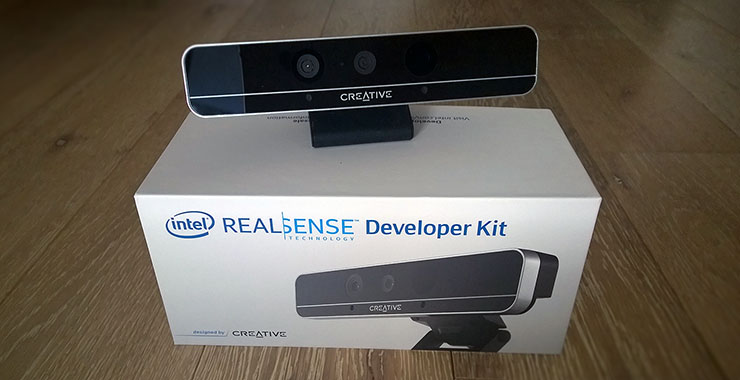
\includegraphics[scale=0.35, angle=0]{Files/Figures/RealSenseCamera.jpg}
    \caption[Η Συσκευή Intel\textregistered\ RealSense\texttrademark{} 3D F200]{Η Συσκευή Intel\textregistered\ RealSense\texttrademark{} 3D F200}
    \label{fig:realsense}
\end{figure}



\section{Επιλογή Εργαλείων Ανάπτυξης}
%ΠΕΣ ΓΙΑ ARUCO,OPENCV,KLP


Πριν το σχεδιασμό μιας εφαρμογής επαυξημένης πραγματικότητας, η διαδικασία επιλογής των κατάλληλων βιβλιοθηκών και εργαλείων λογισμικού που θα χρησιμοποιηθούν, αποτελεί μία σημαντική πτυχή για την πετυχημένη υλοποίηση της εφαρμογής. 


Πέρα από την κατάλληλη επιλογή αισθητήρα χρώματος - βάθους,
πρέπει να επιλεγούν εργαλεία τα οποία θα είναι συμβατά με τον αισθητήρα και τις απαιτήσεις του. Πιο συγκεκριμένα, για τη σωστή λειτουργία του αισθητήρα απαιτείται υπολογιστική μονάδα με επεξεργαστή Intel\textregistered\ Core\texttrademark{} τουλάχιστον 4ης γενιάς και λειτουργικό Windows 8.1 (64bit). Επιπλέον η υπολογιστική μονάδα πρέπει να διαθέτει θύρες USB 3.0 για τη σύνδεση με τον αισθητήρα, ενώ σαν γλώσσες προγραμματισμού υποστηρίζονται οι C++, JavaScript, C\#, Java και Processing.


Για τους παραπάνω λόγους, η υλοποίηση της εφαρμογής έλαβε μέρος σε ένα φορητό υπολογιστή  MacBook Pro με επεξεργαστή Intel\textregistered\ Core\texttrademark{} i5 4278U (2.6GHz) με μνήμη RAM στα 16GB και λειτουργικό σύστημα Windows 8.1 Professional (64bit). Επίσης λόγω της πολυπλοκότητας υλοποίησης απαιτείται η χρήση πολλών διαφορετικών βιβλιοθηκών και η αξιοποίηση των χαρακτηριστικών τους. Για τον ευκολοτερο συνδυασμό των βιβλιοθηκών, χρησιμοποίηθηκε ως IDE το Visual Studio 2010.


Μεταξύ μιας ποικιλίας βιβλιοθηκών επαυξημένης πραγματικότητας, επιλέχθηκε η βιβλιοθήκη ArUco λόγω της απλότητάς της (ανίχνευση markers με μία μόνο γραμμή κώδικα C++) και της δυνατότητας δημιουργίας markerboards που επιτρέπουν την απρόσκοπτη ανίχνευσή τους. Η έκδοση που χρησιμοποιήθηκε (1.2.5) διαθέτει υποστήριξη για διαφορετικές πλατφόρμες (Java, C++, Python) και είναι καλά τεκμηριωμένη (documentation). Επιπλέον διαθέτει ελεύθερη άδεια προς χρήση σε σύγκριση με εργαλεία όπως αυτά που προσφέρουν άλλες εταιρίες όπως η Metaio. Το γεγονός ότι μπορεί εύκολα να συνδυαστεί με την OpenCV και την OpenGL είναι αυτό που συνετέλεσε κυρίως στην επιλογή της.


Οι βιβλιοθήκες λογισμικού που αξιοποιήθηκαν εμφανίζονται παρακάτω:

\begin{description}


\item[OpenGL \& GLUT:] Πρόκειται για μία διαγλωσσική διεπαφή προγραμματισμού εφαρμογών που υποστηρίζει πολλές πλατφόρμες για την απεικόνιση 2D και 3D γραφικών. Χρησιμοποείται στην εφαρμογή μας για την απεικόνιση των εικονικών αντικειμένων πάνω στο βίντεο, το οποίο καταγράφει την πραγματική σκηνή. Παρά το γεγονός ότι θα μπορούσε να χρησιμοποιηθεί μία μηχανή βιντεοπαιχνιδιών όπως η Unity3D για την ευκολότερη διαχείριση των ιδιοτήτων των εικονικών αντικειμένων, επιλέξαμε τη χρήση της OpenGL, προκειμένου να κατανοηθούν οι βασικές τεχνικές που χρησιμοποιούνται στην ανάπτυξη εφαρμογών επαυξημένης πραγματικότητας.



\item[OpenCV (2.4.10):] Γνωστή βιβλιοθήκη προγραμματιστικών συναρτήσεων που έχουν ως στόχο την ανάπτυξη εφαρμογών υπολογιστικής όρασης και την επεξεργασία εικόνας και βίντεο. Η συγκεκριμένη βιβλιοθήκη ανοιχτού κώδικα σχεδιάστηκε για να είναι αποδοτική ώστε να υποστηρίζει εφαρμογές πραγματικού χρόνου, ενώ υποστηρίζει διάφορες πλατφόρμες όπως Windows, Linux, Mac OS X, iOS και Android και διαθέτει διεπαφές για τις γλώσσες C,C++ και Java. 


\item[Qt (5.4)]: Πρόκειται για ένα framework ανάπτυξης που υποστηρίζει πολλές πλατφόρμες για την δημιουργία εφαρμογών, διεπαφών χρηστών (UI) και συσκευών. Για την ανάπτυξη της εφαρμογής σκακιού επαυξημένης πραγματικότητας, χρησιμοποιήθηκαν μόνο οι ιδιότητες της κλάσης QProcess που επιτρέπει την επικοινωνία με εκτελέσιμα αρχεία.


\item[RealSense\texttrademark{} SDK:] Το συγκεκριμένο SDK παρέχει πρόσβαση στα δεδομένα των αισθητήρων χρώματος και βάθους της κάμερας, καθώς επίσης έτοιμους αλγορίθμους για την εξαγωγή blob και περιγραμμάτων (contours), τον εντοπισμό χεριών και την αναγνώριση ομιλίας. 



\end{description}



\section{Πειραματική Εγκατάσταση}

Ο σχεδιασμός και η αρχιτεκτονική του συστήματός μας σχεδιάστηκε έτσι, ώστε ο αισθητήρας Realsense 3D να μπορεί να τοποθετηθεί πάνω σε ένα HMD όπως το Oculus Rift. Μέσα από το HMD οι χρήστες θα μπορούσαν να δουν την έγχρωμη εικόνα της πραγματικής σκηνής που καταγράφει η RealSense\texttrademark{} κάμερα. Έτσι ουσιαστικά θα μπορούσαμε να δημιουργούμε μία συσκευή video see-through display. Ωστόσο λόγω χρονικών και περιορισμών και πολυπλοκότητας, αποφασίστηκε ότι η ενσωμάτωση του Oculus Rift στην αρχιτεκτονική της εφαρμογής θα ήταν υπερβολική. 


Συνεπώς, η συγκεκριμένη εφαρμογή ορίστηκε σε ένα πλαίσιο πειραματικής εγκατάστασης που προσομοιώνει ωστόσο τις παραμέτρους του ύψους και της γωνίας θέασης ενός χρήστη αν τοποθετούσε τον αισθητήρα επάνω σε ένα HMD. Επομένως οι αλγόριθμοι που αναπτύχθηκαν και παρουσιάζονται στη συνέχεια, μπορούν να λειτουργήσουν άψογα αν στο μέλλον ενσωματωθεί ο αισθητήρας σε ένα HMD όπως το Oculus Rift. 


Με στόχο να μπορούμε να αλληλεπιδράσουμε με το εικονικό περιεχόμενο και να αλληλεπιδράσουμε με βάση τη χειρονομία "τσιμπήματος", ορίσαμε μία περιοχή δοκιμών, όπου το markerboard τοποθετείται επάνω σε ένα τραπέζι και είναι εύκολα προσβάσιμο από έναν χρήστη που κάθεται μπροστά του. 


\begin{figure}[H]
    \centering
    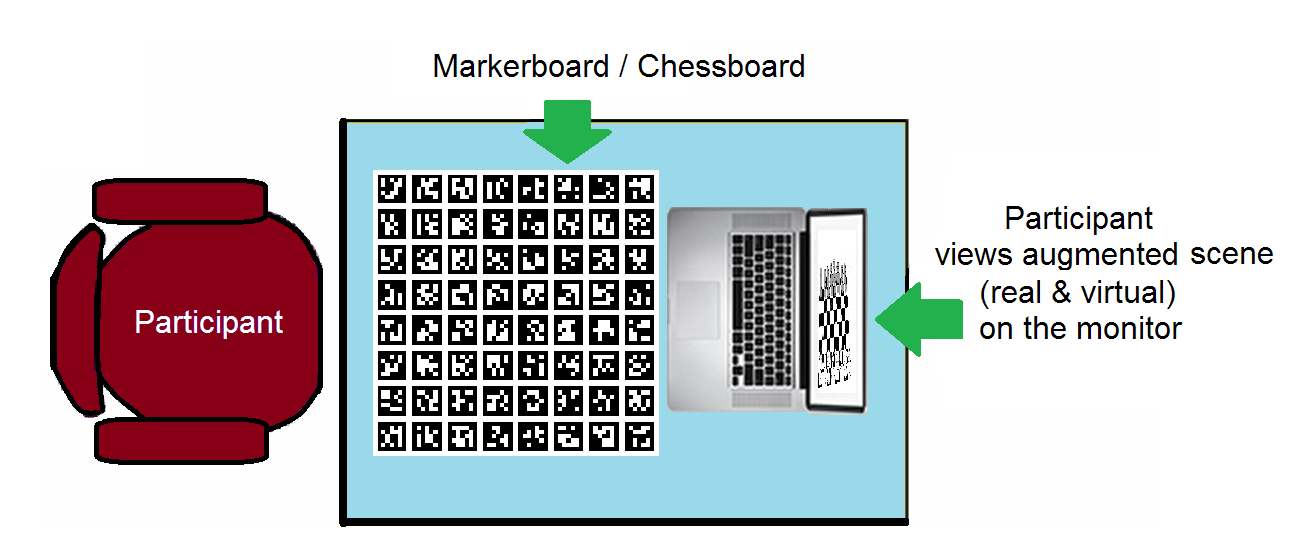
\includegraphics[scale=0.8, angle=0]{Files/Figures/planviewoftheexperimentalsetup.png}
    \caption[Κάτοψη της σχεδιασμού της πειραματικής εγκατάστασης]{Κάτοψη της σχεδιασμού της πειραματικής εγκατάστασης}
    \label{fig:ps3game}
\end{figure}


Η κάμερα RealSense\texttrademark{} 3D τοποθετείται στο πίσω μέρος ενός απλού καπέλου το οποίο φοράει ο χρήστης κατά τη διάρκεια των δοκιμών, εμπνευσμένο από παλαιότερη εργασία \cite{Mathews2007}. Όσο ο χρήστης φορά το καπέλο με τον αισθητήρα, ο αισθητήρας βλέπει προς το markerboard με αποτέλεσμα να "κοιτά" προς την περιοχή της αλληλεπίδρασης. Τέλος, ένας φορητός υπολογιστής τοποθετείται μπροστά από το markerboard και το χρήστη, ώστε να μπορεί να δει το επαυξημένο video που καταγράφει η κάμερα. Η κάμερα είναι συνδεδεμένη με το φορητό υπολογιστή, στον οποίο τρέχει η εφαρμογή. Η εικόνα~\ref{fig:test} δείχνει την πειραματική εγκατάσταση και έναν χρήστη κατά τη διάρκεια δοκιμής της εφαρμογής.



\begin{figure}[H]
\begin{subfigure}{.5\textwidth}
  \centering
  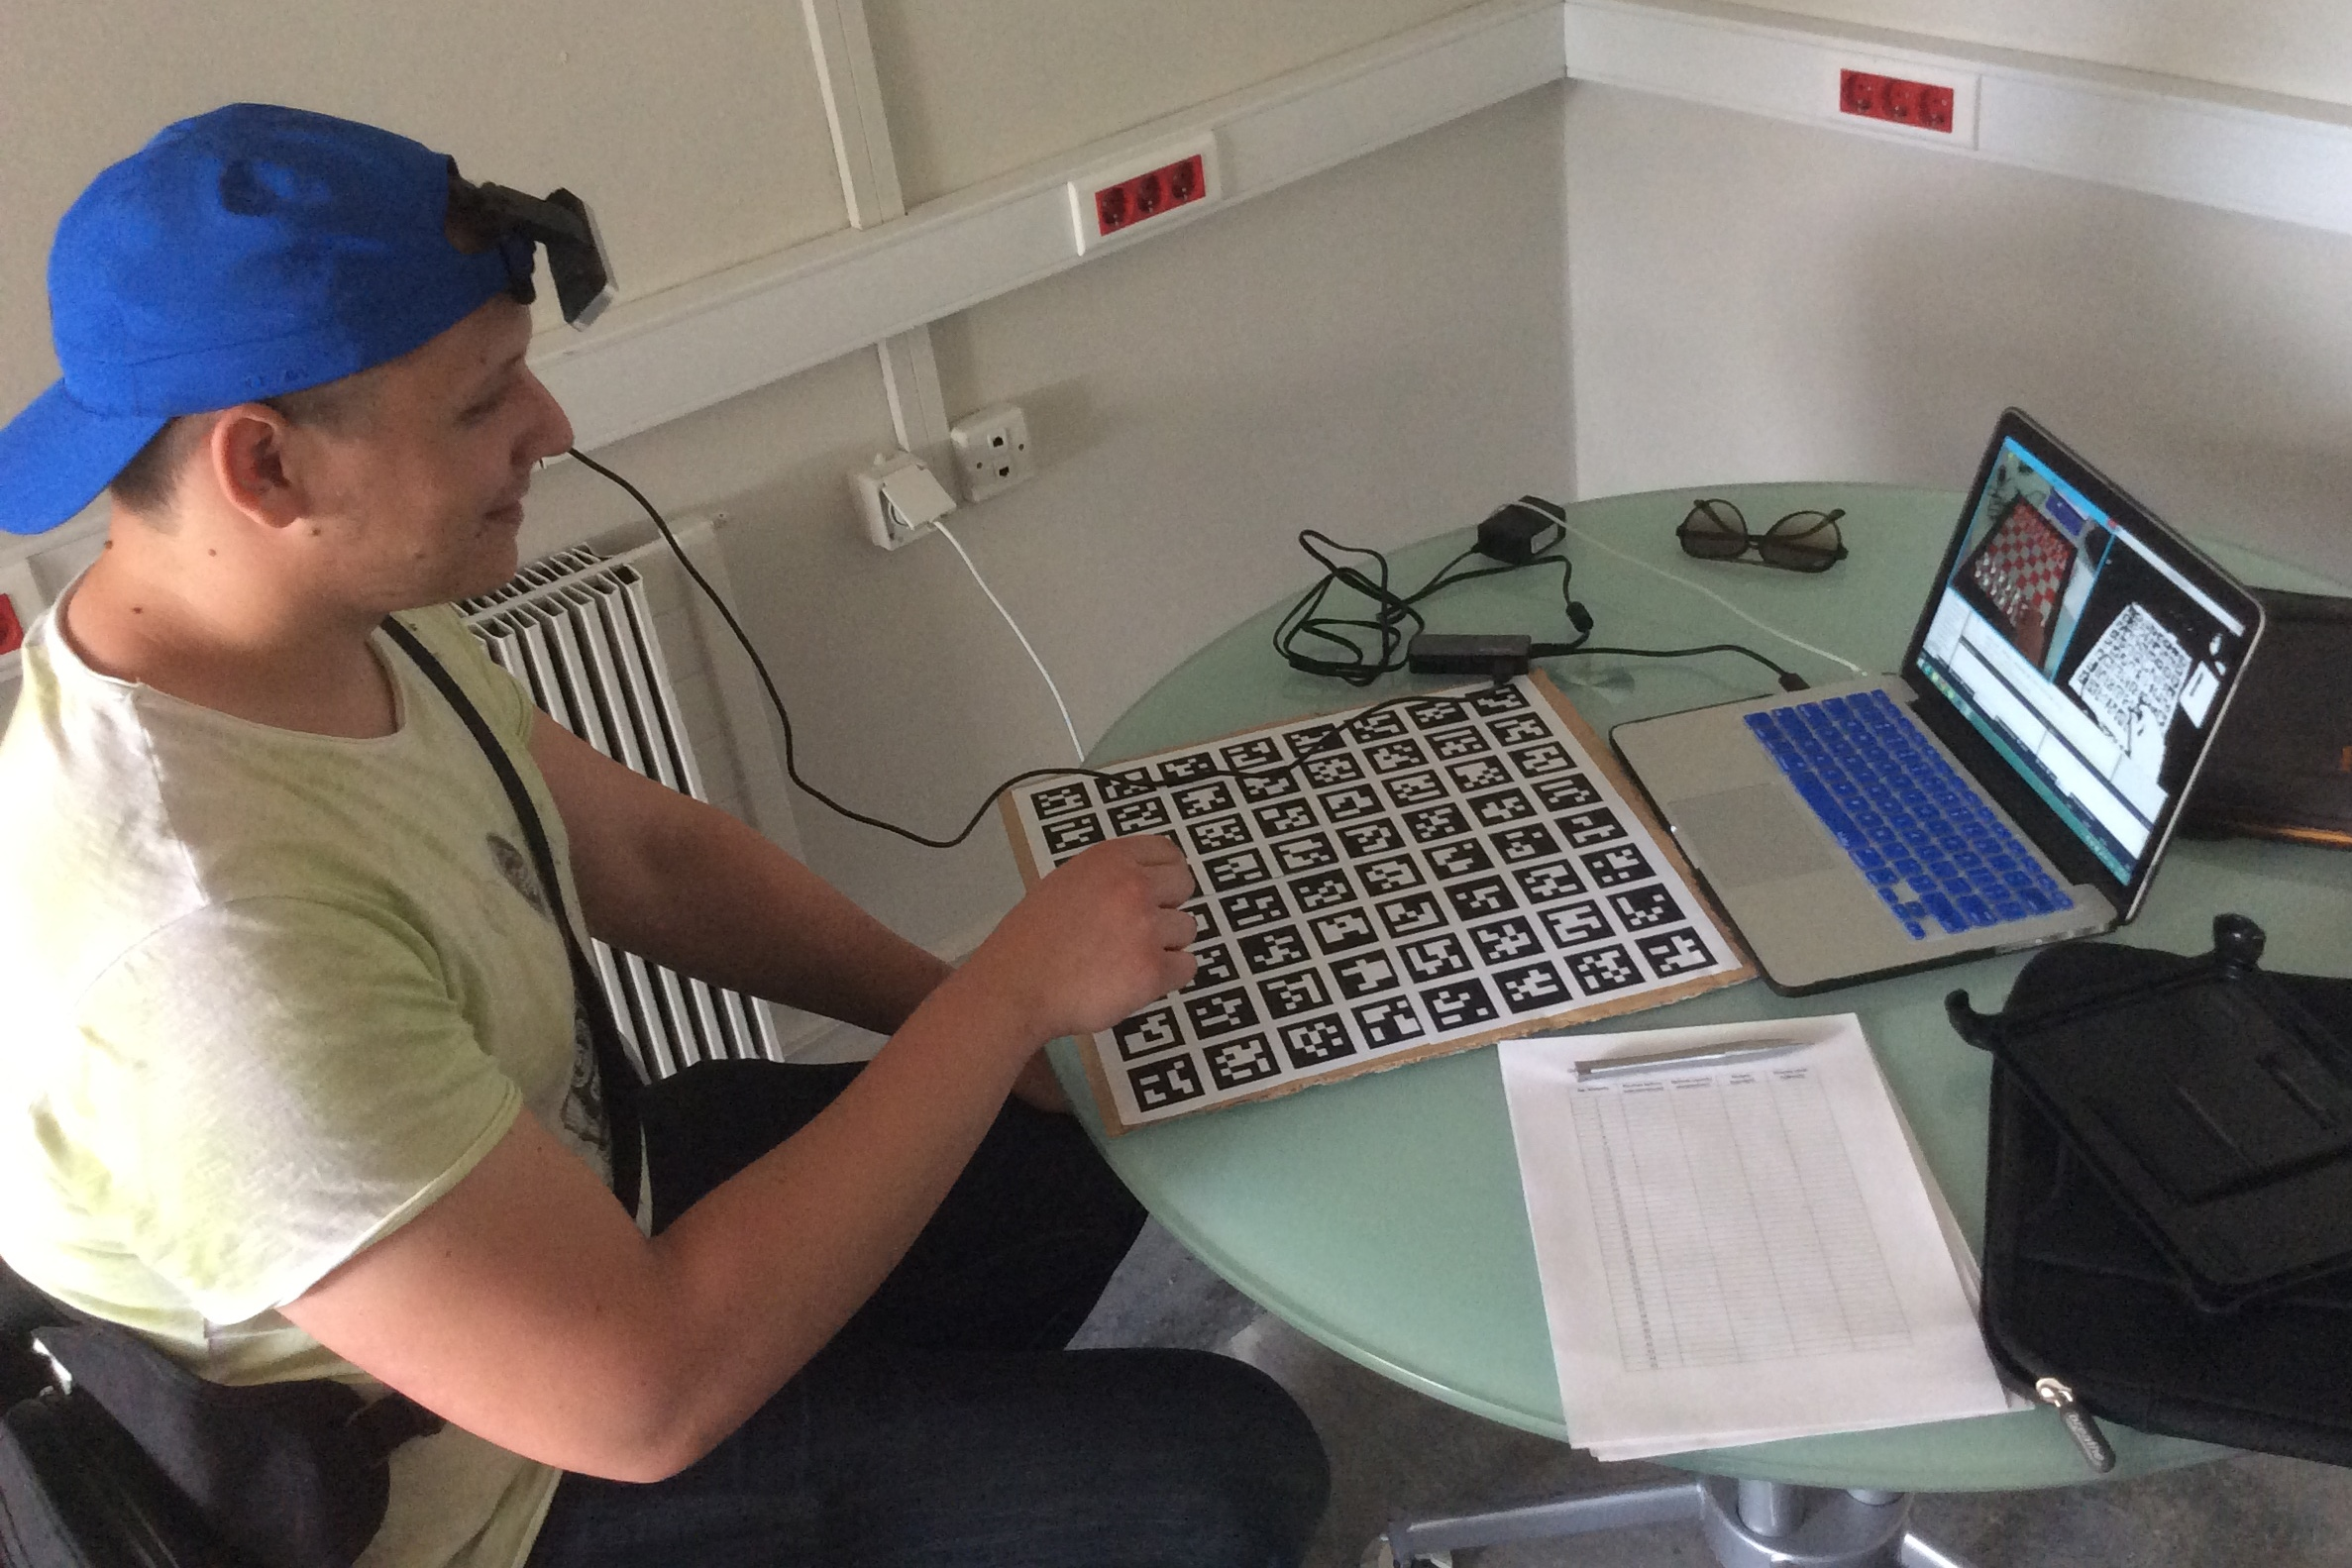
\includegraphics[width=.8\linewidth]{Files/Figures/user1.png}
  \caption{1a}
  \label{fig:sfig1}
\end{subfigure}%
\begin{subfigure}{.5\textwidth}
  \centering
  \includegraphics[width=.7\linewidth]{Files/Figures/user2.png}
  \caption{1b}
  \label{fig:sfig2}
\end{subfigure}\\
\caption{Φωτογραφία χρήστη κατά τη διάρκεια των δοκιμών}
\label{fig:test}
\end{figure}



\section{Βαθμονόμηση της Κάμερας}




Στα πλαίσια της διπλωματικής εργασίας απαιτείται η χρήση μιας απλής μεθόδου με αξιοποίηση συνηθισμένου εξοπλισμού για την βαθμονόμηση. Η διαδικασία της βαθμονόμησης απλοποιείται χρησιμοποιώντας ένα υπολογιστικό εργαλείο της OpenCV. 
Η διαδικασία περιλαμβάνει την καταγραφή ενός συνόλου φωτογραφιών ενός calibration board, και ο αλγόριθμος του εργαλείου υπολογίζει τις εσωτερικές παραμέτρους.
Το εργαλείο βαθμονόμησης αποθηκεύει τα αποτελέσματα σε ένα αρχείο, το οποίο διαβάζει η εφαρμογή επαυξημένης πραγματικότητας στην αρχή της εκτέλεσής της. 



%σκακιερα
Η OpenCV διαθέτει έτοιμες συναρτήσεις και εργαλεία για την βαθμονόμηση της κάμερας που βασίζονται σε μεθόδους που αναφέρθηκαν στο κεφάλαιο \ref{c:2}. Επιπλέον μέσω της OpenCV μπορούμε να μάθουμε τους συντελεστές παραμόρφωσης της κάμερας. 
Καταφεύγουμε λοιπόν, στη λύση του εργαλείου της Opencv για την βαθμονόμηση της κάμερας \cite{calibrationtool}, που προσφέρει μία έτοιμη και αποτελεσματική λύση, με χρήση μίας απλής κάμερας και μιας απλής επίπεδης εικόνας και συγκεκριμένα του μοτίβου τετραγώνων σκακιέρας, η οποία χρειάζεται απλά να εκτυπωθεί σε απλό χαρτί. 




Για τη διεξαγωγή της βαθμονόμησης απαιτείται η χρήση μιας απλής, επίπεδης εικόνας ασπρόμαυρης σκακιέρας, που μπορεί να εκτυπωθεί με ένα κοινό εκτυπωτή. Η διαδικασία αυτή είναι αυτόματη, ενώ τα μόνα δεδομένα εισόδου που θα πρέπει να δώσουμε στο εργαλείο της OpenCV είναι ο αριθμός των εσωτερικών γωνιών των τετραγώνων της. Για παράδειγμα το πρότυπο της βαθμονόμησης φαίνεται στο σχήμα~\ref{fig:pattern}, όπου έχουμε μία σκακιέρα, με αριθμό διαστάσεων με βάση τις εσωτερικές γωνίες 7x6. Η πληροφορία αυτή αξιοποιείται μέσω μεθόδων της OpenCV και επιστρέφονται ο πίνακας των εσωτερικών παραμέτρων της κάμερας και οι συντελεστές παραμόρφωσης. 


\begin{figure}[H]
\begin{subfigure}{.5\textwidth}
  \centering
  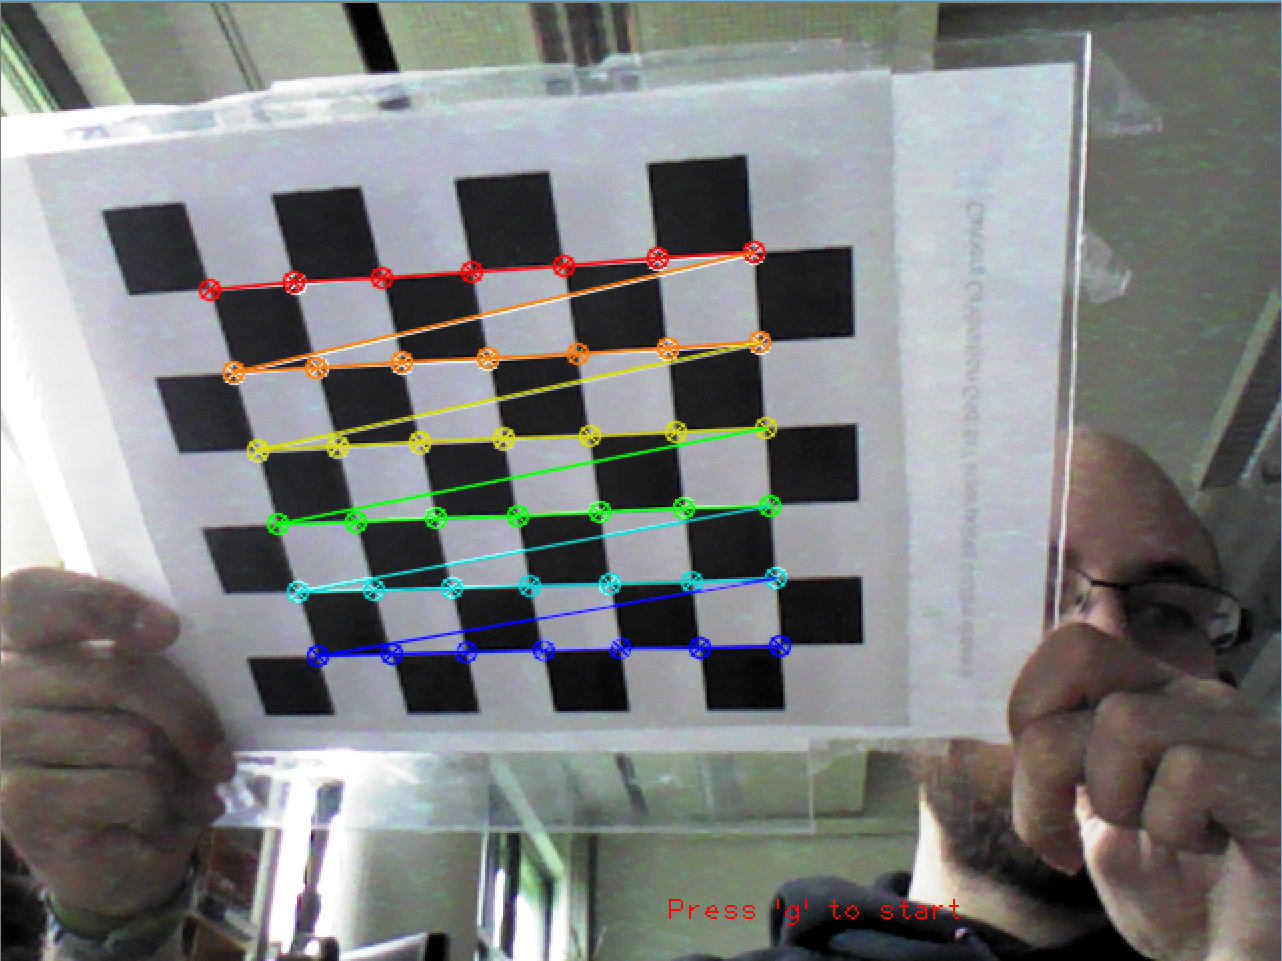
\includegraphics[width=.8\linewidth]{Files/Figures/calibration.png}
  \caption{1a}
  \label{fig:calibration_screenshot1}
\end{subfigure}%
\begin{subfigure}{.5\textwidth}
  \centering
  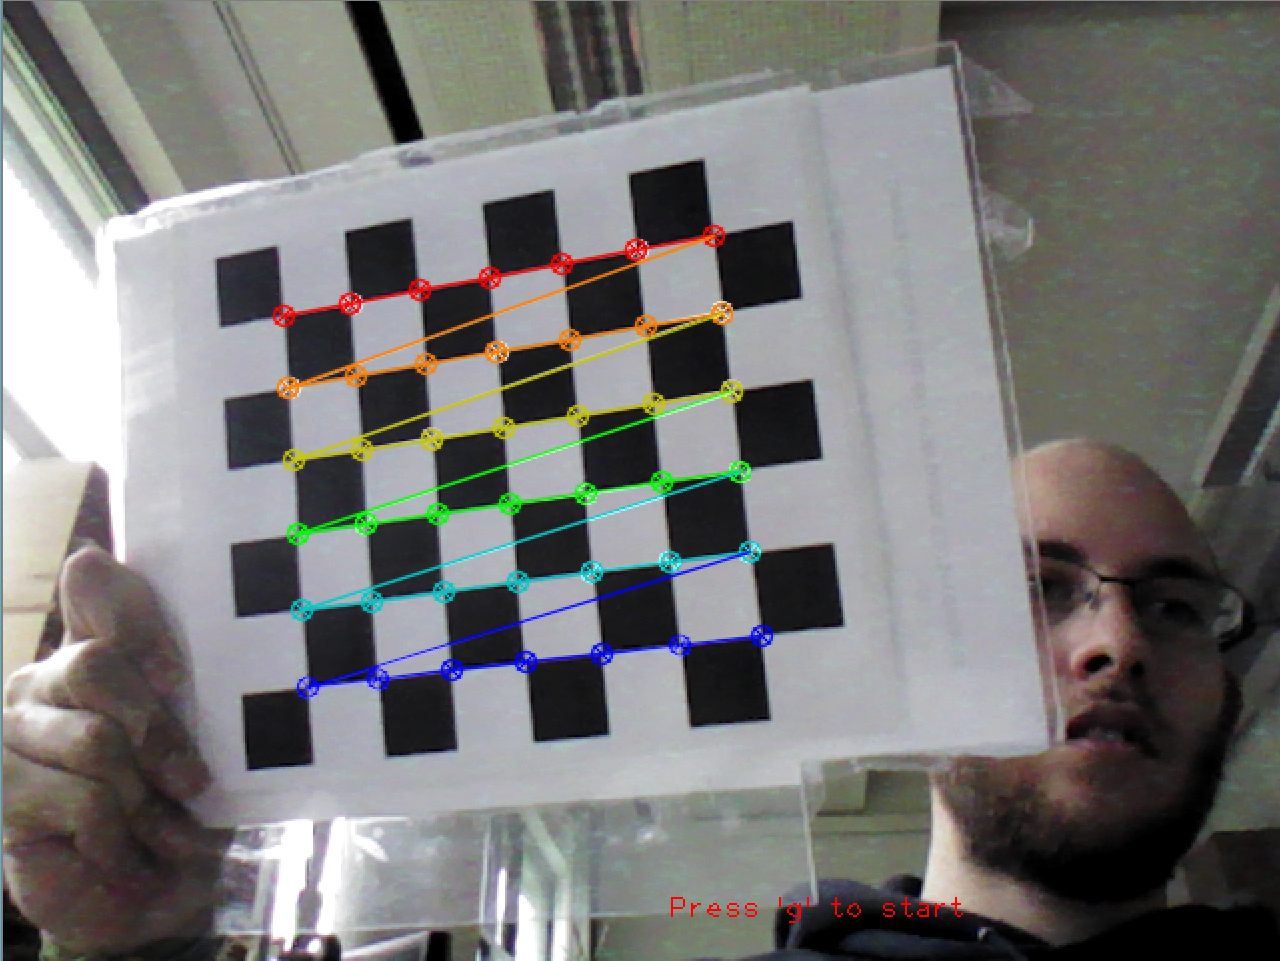
\includegraphics[width=.8\linewidth]{Files/Figures/calib2.png}
  \caption{1b}
  \label{fig:calibration_screenshot2}
\end{subfigure}
\caption[Στιγμιότυπο κατά τη διαδικασία της βαθμονόμησης κάμερας μέσω της OpenCV]{Στιγμιότυπο κατά τη διαδικασία της βαθμονόμησης κάμερας μέσω της OpenCV}
\label{fig:calibration_screenshot}
\end{figure}



Η βαθμονόμηση της κάμερας πραγματοποιείται μόνο μία φορά σαν αρχικό βήμα (offline calibration) κατά το αρχικό στάδιο της ανάπτυξης της εφαρμογής. Πιο συγκεκριμένα, κάνουμε ξεχωριστό calibration για κάθε διαφορετικό μοντέλο κάμερας που μπορεί να χρησιμοποιηθεί στην αναπτυσσόμενη εφαρμογή, καθώς και για κάθε διαφορετική ανάλυση αυτών. Το αποτέλεσμα είναι ένα ξεχωριστό αρχείο για κάθε κάμερα και κάθε ανάλυση που περιέχει τις αντίστοιχες εσωτερικές παράμετρους. Ανάλογα με τον εξοπλισμό και τις επιλογές του χρήστη φορτώνεται κατά την έναρξη της εφαρμογής το ανάλογο αρχείο. Έτσι οι εσωτερικές παράμετροι είναι γνωστές, ώστε σε μεταγενέστερο στάδιο να βρεθούν οι εξωτερικές παράμετροι.



\begin{figure}[H]
    \centering
    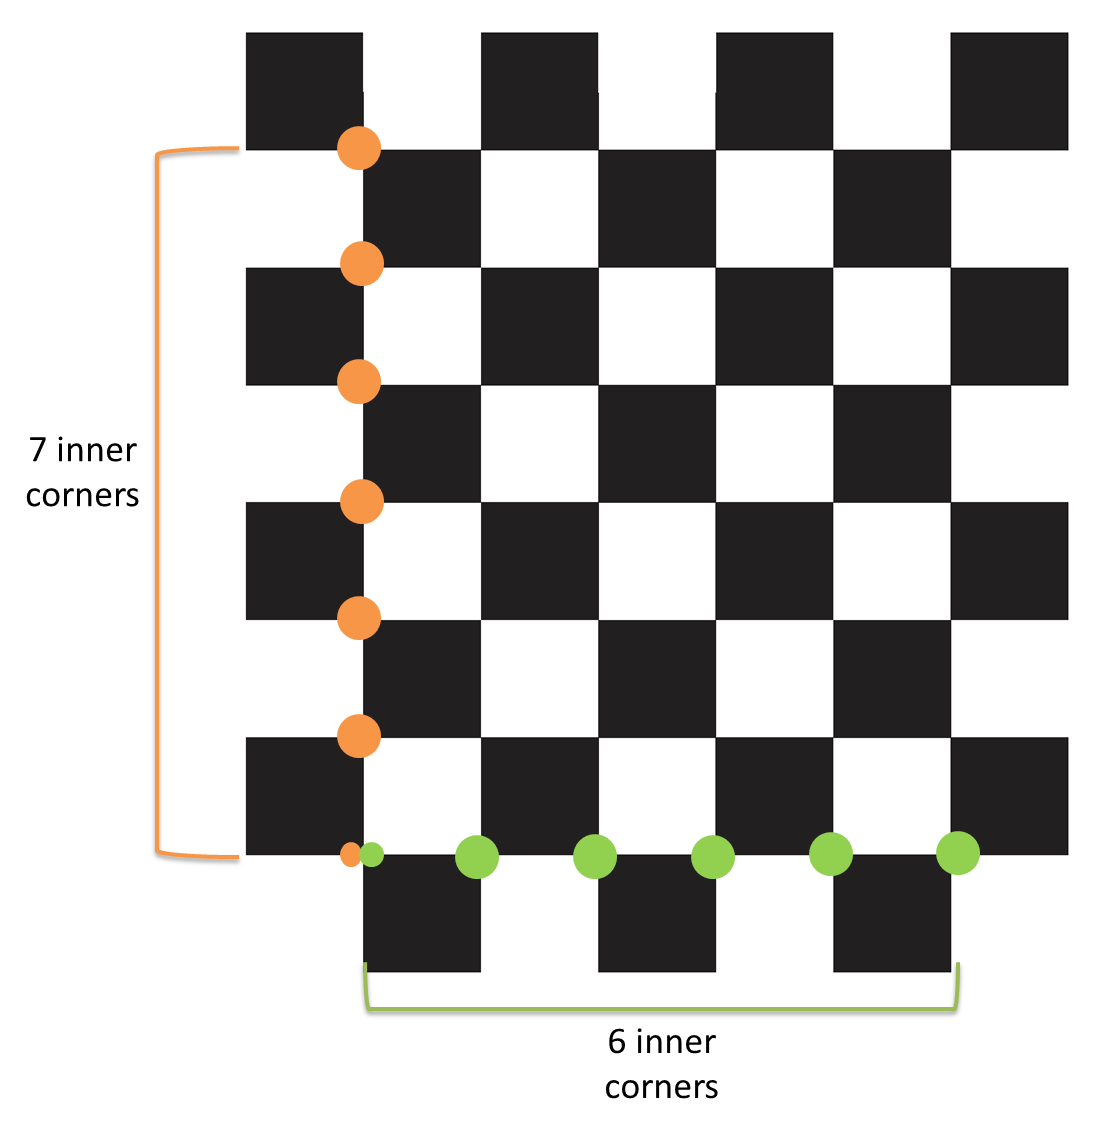
\includegraphics[scale=0.3, angle=0]{Files/Figures/pattern.png}
    \caption[Πρότυπο σκακιέρας για τη βαθμονόμησης της κάμερας]{Πρότυπο σκακιέρας για τη βαθμονόμησης της κάμερας}
    \label{fig:pattern}
\end{figure}




Στο πλαίσιο της παρούσας εργασίας, έγινε βαθμονόμηση με λήψη εικόνων επίπεδης σκακιέρας με μέγεθος 7 x 6 εσωτερικών γωνιών, με χρήση του παραδείγματος της βιβλιοθήκης OpenCV. Το μέγεθος κάθε τετραγώνου της σκακιέρας ορίστηκε στα 2,5cm. Το πρότυπο αυτό καταγράφηκε μέσω της κάμερας σε 25 διαφορετικές θέσεις. Η κάμερα διατηρήθηκε σε σταθερό σημείο και μετακινήσαμε την εκτυπωμένη εικόνα της σκακιέρας σε διαφορετικές θέσεις και με διαφορετικές κλίσεις. 






Η διαδικασία της βαθμονόμησης σε ανάλυση 640 x 480 έδωσε σαν αποτέλεσμα τις παρακάτω εσωτερικές παραμέτρους:


\begin{equation}
K=
\begin{bmatrix}
603.77848970443176 & 0 & 319.5\\
0 & 603.77848970443176 & 239.5\\
0 & 0 & 1
\end{bmatrix}
\end{equation}

Βλέποντας τις τιμές των principal points $c_{x}=319.5$ and $c{y}=239.5$ παρατηρούμε ότι είναι περίπου στο κέντρο των επιλεγμένων διαστάσεων δηλαδή κοντά στις τιμές  320 (640/2) και 240 (480/2). Επίσης βλέπουμε ότι $f_{x}=f_{y}$ που σημαίνει ότι χρησιμοποιείται κοινή εστιακή απόσταση και για τους 2 άξονες.


Εξ ορισμού η OpenCV μας δίνει 5 συντελεστές παραμόρφωσης, 3 ακτινικούς και 2 εφαπτομενικούς. Συγκεκριμένα κατά τη βαθμονόμηση πήραμε:

\begin{equation}
\begin{aligned}
k1= 0.16901284929874760\\
k2= -1.0214355567073656\\
p1= 0\\
p2= 0\\
k3= 1.3599972288823818 
\end{aligned}
\end{equation}

Το σφάλμα επαναπροβολής (Re-projection error) δίνει μία καλή εκτίμηση της ακρίβειας των παραμέτρων που βρέθηκαν κατά τη βαθμονόμηση της κάμερας. Η τιμή του πρέπει να είναι όσο γίνεται πιο κοντά στο 0 και υπολογίζεται με βάση τους πίνακες εσωτερικών παραμέτρων, συντελεστών παραμόρφωσης, περιστροφής και μετατόπισης. 


Μετά τη διαδικασία βαθμονόμησης το σφάλμα που πήραμε ήταν πολύ κοντά στο 0 και συγκεκριμένα :

\begin{equation}
Avg_{Reprojection_Error} = 0.20315774320090751
\end{equation}


\section{Δημιουργία Markerboard}
%ΑΝΑΛΥΣΕ ΤΟ ARUCO FEATURE KAI ΠΩΣ ΓΙΝΕΤΑΙ ΤΟ MARKER TRACKING ΑΠΟ ΤΗΝ ARUCO ΚΑΙ ΤΟ BOARD.

Ως επαύξηση της πραγματικότητας ορίζεται η διαδικασία πρόσθεσης εικονικής πληροφορίας σε εικόνες ή βίντεο. Για να συμβεί κάτι τέτοιο, πρέπει να γνωρίζουμε που ακριβώς πρέπει να απεικονιστεί η εικονική πληροφορία. Παρά το γεγονός ότι ορισμένες εφαρμογές αξιοποιούν τα φυσικά χαρακτηριστικά μιας σκηνής όπως η υφή ή σημεία κλειδιά, τα markers αποτελούν ακόμα έναν ελκυστικό τρόπο προσέγγισης επειδή είναι εύκολη η γρήγορη ανίχνευσή τους και η ακρίβεια που μπορεί να επιτευχθεί, όπως παρουσιάστηκε και στο~\ref{ssec:markerpose}. Μέσω της ανίχνευσης ενός marker όπως αυτοί που χρησιμοποιούνται από την ArUco μπορούν να υπολογιστούν οι εξωτερικές παράμετροι της κάμερας, δηλαδή η θέση και ο προσανατολισμός της σε σχέση με το marker ώστε να γνωρίζει το πρόγραμμα που πρέπει να σχεδιάσει τα 3D αντικείμενα και που είναι η αρχή των αξόνων (0,0,0) του συστήματος κοσμικών συντεταγμένων της σκηνής. 



Το γνωστό επιτραπέζιο παιχνίδι του σκακιού απαιτεί τη χρήση μιας σκακιέρας ως βάση προκειμένου να τοποθετηθούν τα πιόνια επάνω της. Kατά τη διάρκεια ενός παιχνιδιού σκακιού, ο χρήστης συχνά πρέπει να μετακινεί τα πιόνια με το χέρι του. Όταν συμβαίνει αυτό, το χέρι του χρήστη περνά πάνω από τη σκακιέρα αποκρύπτοντας ένα αρκετά σημαντικό μέρος της. 


Στα πλαίσια της παρούσας διπλωματικής εργασίας και προκειμένου να δημιουργήσουμε ένα σκάκι επαυξημένης πραγματικότητας θεωρήθηκε ότι η αξιοποίηση ενός markerboard προσομοιώνει τις ιδιότητες μιας σκακιέρας, ενώ η απόκρυψη μέρους του markerboard από το χέρι του χρήστη δεν επηρεάζει την απεικόνιση των εικονικών πιονιών κατά τη διάρκεια της μετακίνησης ενός πιονιού από το χρήστη. Επομένως αποφασίστηκε η δημιουργία ενός markerboard με μια διάταξη από 64 markers, σε ένα πλέγμα 8x8, με διαστάσεις ίδιες με αυτές μιας σκακιέρας. 


Οι δημιουργοί της βιβλιοθήκης ArUco δημοσίευσαν μία επιστημονική εργασία \cite{garrido2014automatic} όπου αναλύεται η μεθοδολογία για τη δημιουργία markerboard με markers τα στα οποία αντιστοιχίζονται συγκεκριμένα IDs με στόχο τον υψηλό αριθμό μεταβολών bits ώστε να μην μπερδεύονται τα markers με πραγματικά αντικείμενα του περιβάλλοντος, να ανιχνεύονται, δηλαδή, ευκολότερα από το σύστημα. 

Προτείνεται λοιπόν μια αυτόματη μέθοδος για την παραγωγή ενός markerboard με τον επιθυμητό αριθμό markers και τον επιθυμητό αριθμό bits. Χρησιμοποιώντας το έτοιμο εργαλείο που παρέχεται από τη βιβλιοθήκη ArUco για το σκοπό αυτό, δημιουργήσαμε μία "σκακιέρα" από markers υψηλής αξιοπιστίας, όπως φαίνεται και στην εικόνα~\ref{fig:markerboard}




\begin{figure}[H]
    \centering
    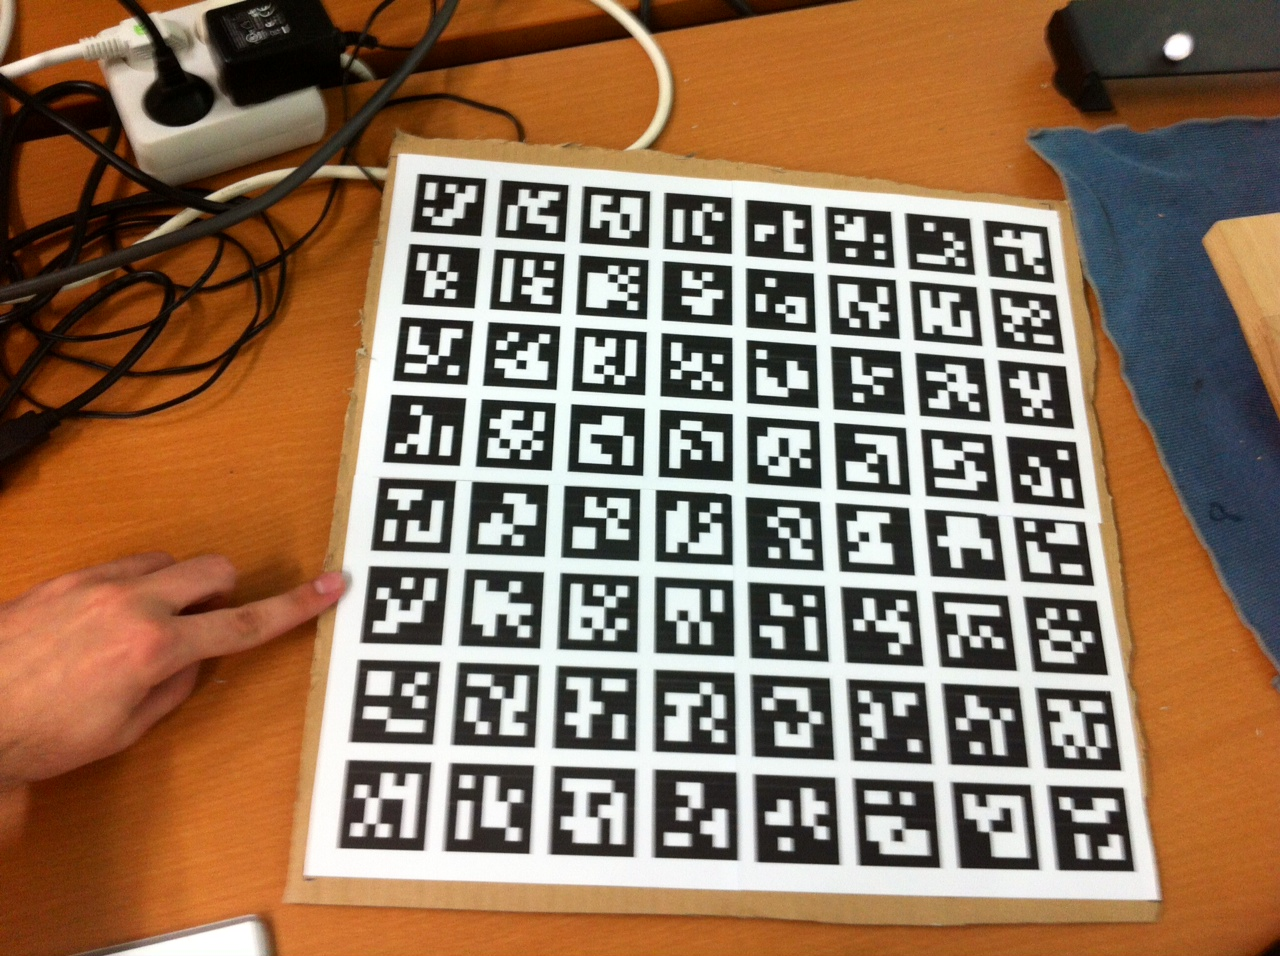
\includegraphics[width=0.5\textwidth]{Files/Figures/markerboard.jpg}
    \caption[Το markerboard που δημιουργήθηκε μέσω της ArUco]{Το markerboard που δημιουργήθηκε μέσω της ArUco}
    \label{fig:markerboard}
\end{figure}




\section{Ανίχνευση Θέσης Χειρονομίας "Τσιμπήματος"} \label{section:pinch}
%\section{Αναγνώριση Χειρονομίας Τσιμπήματος} 
%ΠΩΣ ΑΚΡΙΒΩΣ ΚΑΝΩ ΤΗ ΧΕΙΡΟΝΟΜΙΑ ΤΣΙΜΠΗΜΑΤΟΣ-ΤΑ ΘΕΩΡΗΤΙΚΑ ΜΕΡΗ



Προκειμένου να ορίσουμε τον τρόπο με τον οποίο θα γίνεται ο εντοπισμός των χειρονομιών, καθώς και το είδος των χειρονομιών που πρέπει να ανιχνευτούν, χρειάζεται να καθοριστούν οι απαιτήσεις του συστήματος με λεπτομέρειες.
Για να αναπτυχθεί ένα σκάκι επαυξημένης πραγματικότητας, απαιτείται προφανώς αλληλεπίδραση σε πραγματικό χρόνο, σχετικά φθηνός εξοπλισμός και αλληλεπίδραση με όσο περισσότερο φυσικό τρόπο γίνεται, δηλαδή χωρίς τη χρήση ειδικών γαντιών ή καλωδίων. 

Οι απαιτήσεις του συστήματος για εκτέλεση των αλληλεπιδράσεων σε πραγματικό χρόνο, περιορίζει το επίπεδο της ανίχνευσης χειρονομιών που μπορεί να επιτευχθεί, ενώ παράλληλα οι απαιτήσεις για εξοπλισμό χαμηλού κόστους περιορίζουν την ποιότητα της εικόνας που πρέπει να καταγραφεί. Ο τρίτος περιορισμός που εισάγεται, προϋποθέτει τη χρήση τεχνικών όρασης υπολογιστών για την αναγνώριση των χειρονομιών του χρήστη, η απόδοση των οποίων περιορίζεται από τον επεξεργαστή του συστήματος. 



Η χειρονομία "τσιμπήματος" είναι μία χειρονομία που μπορεί να χρησιμοποιηθεί για την αλλεπίδραση με αντικείμενα στον τρισδιάστατο χώρο. Η χειρονομία "τσιμπήματος" μπορεί να πραγματοποιηθεί αρκετές φορές και υποδηλώνει φυσική κίνηση για επιλογή ενός αντικειμένου. Επομένως η αναγνώρισή της είναι βασική προϋπόθεση για την υλοποίηση βασικών αλληλεπιδράσεων με τα εικονικά αντικείμενα. 


Κατά τη διάρκεια της μετακίνησης ενός πιονιού στο σκάκι, μέρος του χεριού και των δακτύλων του χρήστη δεν είναι ορατά από την κάμερα. Για το λόγο αυτό, σκεφτήκαμε ότι η χρήση τεχνικών εντοπισμού της πόζας του χεριού μέσω ενός σκελετικού μοντέλου ή μέσω των μεθόδων που παρέχονται από το RealSense\texttrademark{} SDK θα ήταν υπερβολική για το συγκεκριμένο είδος εφαρμογής. Επομένως, δε χρειάζεται να ανιχνεύσουμε ούτε ολόκληρο το χέρι του χρήστη, ούτε τα δάκτυλα του αυτούσια. 



Με βάση τους παραπάνω περιορισμούς, η ανάπτυξη του συστήματος που αναπτύσσεται στην παρούσα διπλωματική εργασία, βασίστηκε στην εργασία του Andrew Wilson \cite{Wilson2006}, όπου παρουσιάζεται μία τεχνική υπολογιστικής όρασης για την εύκολη και γρήγορη αναγνώριση της κίνησης κατά την οποία ο αντίχειρας και ο δείκτης ενός χρήστη έρχονται κοντά (χειρονομία "τσιμπήματος") για εφαρμογές μικρής εμβέλειας και σχετικά ελεγχόμενες συνθήκες θέασης. Η τεχνική αυτή αποφεύγει πολύπλοκους και εύθραυστους αλγορίθμους εντοπισμού των χεριών, εντοπίζοντας την οπή που σχηματίζεται όταν ο δείκτης αγγίζει τον αντίχειρα του χρήστη. Το πρόβλημα της αλληλεπίδρασης μετατρέπεται ουσιαστικά σε πρόβλημα αναγνώρισης χειρονομιών. Περιγράφεται, δηλαδή, ένας εύκολος και γρήγορος τρόπος για την αναγνώριση της χειρονομίας τσιμπήματος. 


Συγκεκριμένα, υλοποιήθηκε ένα αλγόριθμος ανίχνευσης χειρονομιών, ο οποίος ενεργοποιεί μία εντολή αρπαγής και απελευθέρωσης των εικονικών πιονιών στην σκηνή της επαυξημένης πραγματικότητας. Χρησιμοποιούμε αυτή τη χειρονομία για να επιλέξουμε ένα πιόνι στη σκακιέρα και να μπορέσουμε να το μετακινήσουμε σε κάποια άλλη θέση.


Για να απλοποιηθεί αυτή η διαδικασία, πρέπει να οριστουν ορισμένες παραδοχές.
Πρώτα απ' όλα, το σύστημα θα πρέπει να χρησιμοποιείται με το δεξί χέρι του χρήστη, αν και μπορεί μελλοντικά να λυθεί αυτό το πρόβλημα εύκολα. Επιπλέον, η χειρονομία τσιμπήματος πρέπει να πραγματοποιείται με την ένωση του αντίχειρα και του δείκτη, αλλά και με τα υπόλοιπα δάκτυλα να είναι τεντωμένα και όσο γίνεται πιο κάθετα στο δείκτη, όπως φαίνεται στην εικόνα~\ref{fig:gesture_rec}.

\begin{figure}[H]
    \centering
    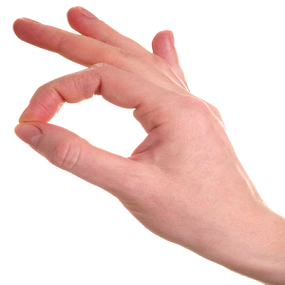
\includegraphics[scale=0.6, angle=0]{Files/Figures/correct_pinch.jpg}
    \caption[Παράδειγμα παραδοχής για τη σωστή χειρονομία "τσιμπήματος"]{Παράδειγμα παραδοχής για τη σωστή χειρονομία "τσιμπήματος"}
    \label{fig:gesture_rec}
\end{figure}



Οι συναρτήσεις του SDK επιτρέπουν την ανίχνευση αντικειμένων μπροστά από την κάμερα, όπως είναι τα blobs και την εξαγωγή περιγραμμάτων και σημείων ενδιαφέροντος για αυτά τα blobs. Η ανίχνευση των blobs είναι μία εναλλακτική που βολεύει σε σχέση με τον εντοπισμό των χεριών που παρέχει το SDK, αφού η εφαρμογή μας δεν απαιτεί την ανίχνευση και τον εντοπισμό χεριών. Κάθε blob διαθέτει μία εξωτερική γραμμή περιγράμματος (contour line) και ανάλογα με στο σχήμα του blob, μία ή περισσότερες εσωτερικές γραμμές περιγράμματος. Κάθε τέτοια γραμμή περιγράμματος αναπαρίσταται από μία σειρά σημείων. Οι εξωτερικές γραμμές περιγραμμάτων (εξωτερικά σύνορα), καθώς και οι εσωτερικές γραμμές των περιγραμμάτων ορίζονται από ένα πίνακα σημείων.


Η προσέγγιση μας, αξιοποιεί τα δεδομένα των blobs και την οπή που σχηματίζεται όταν ο αντίχειρας ακουμπά ή βρίσκεται πολύ κοντά στον δείκτη. Πιο συγκεκριμένα, υλοποιήθηκε ένας αλγόριθμος που ανιχνεύει πότε λαμβάνει χώρα μία χειρονομία τσιμπήματος και που ακριβώς στον 3D χώρο. Γνωρίζοντας το σημείο στο 3D χώρο στο οποίο συμβαίνει η χειρονομία, μπορούμε να επιλέξουμε το σωστό πιόνι και να το μετακινήσουμε ανάλογα. 


Η απρόσκοπτη ανίχνευση μιας χειρονομίας τσιμπήματος είναι η βάση για τη σωστή λειτουργία του συστήματός μας και για αυτό το λόγο θα αναφερθούμε ξεχωριστά στην αναγνώριση και την ανίχνευση της θέσης στην οποία πραγματοποιείται η χειρονομία. Ο αλγόριθμος που σχεδιάστηκε αναλύεται στη συνέχεια.



Σε κάθε frame, παίρνουμε τις εικόνες βάθους και χρώματος που καταγράφει η συσκευή. Λόγω της λανθασμένης ευθυγράμμισης και της φυσικής απόκλισης της θέσης του αισθητήρα χρώματος σε σχέση με τον αισθητήρα βάθους (αφού δεν βρίσκονται ο ένας πάνω στον άλλο), χρειάζεται ένας τρόπος να αντιστοιχηθούν τα εικονοστoιχεία χρώματος με τα εικονοστοιχεία βάθους και αντίστροφα. Για το συγκεκριμένο λόγο, η βιβλιοθήκη RealSense παρέχει μία δομή με το όνομα UVMap η οποία επιτελεί αυτό το συγκεκριμένο σκοπό.

Στην αρχή της διαδικασίας, χρειάζεται να χρησιμοποιήσουμε τις ιδιότητες της βιβλιοθήκης για εξαγωγή των blobs. Πριν συμβεί αυτό, πρέπει να ορίσουμε κάποιες παραμέτρους, όπως τον μέγιστο αριθμό blobs που θέλουμε να ανιχνευτούν και το επίπεδο της εξομάλυνσης κατά την κατάτμηση της εικόνας για να πάρουμε τα σωστά περιγράμματα του blob. 

Στην προσέγγιση μας, επιλέξαμε να ανιχνεύεται το κοντινότερο blob της εικόνας βάθους ως προς την κάμερα, διότι κατά τη διάρκεια ενός παιχνιδιού σκακιού ως προς το σημείο παρατήρησης του χρήστη (π.χ τα μάτια του), το ρόλο αυτό παίζουν τα χέρια του, τα οποία και όντως θέλουμε να εντοπίσουμε. Μόλις αναγνωριστεί το κοντινότερο blob, ωστόσο, πρέπει να το επεξεργαστούμε για να δούμε αν όντως πρόκειται για ένα blob χεριού ή για κάποιο άλλο αντικείμενο.


\begin{figure}[H]
    \centering
    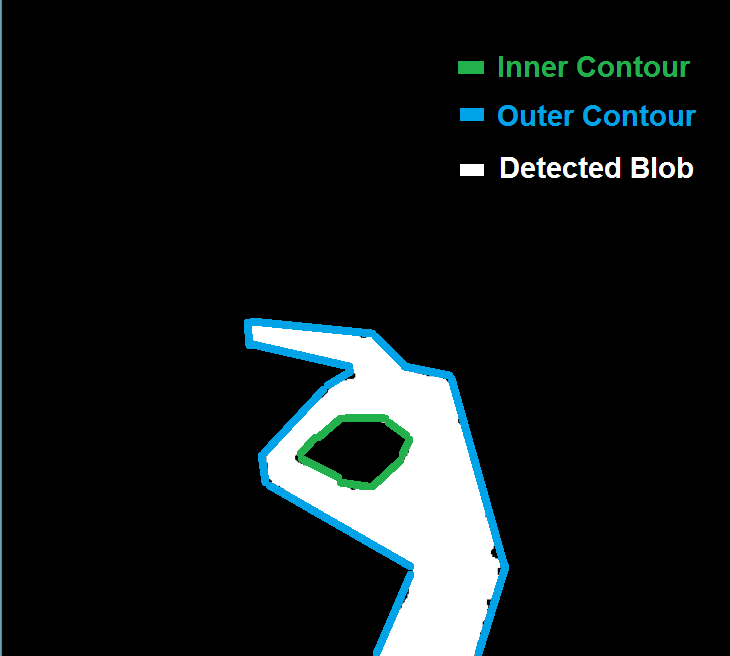
\includegraphics[scale=0.7, angle=0]{Files/Figures/2.png}
    \caption[Παράδειγμα blob χεριού και περιγραμμάτων που σχηματίζονται]{Παράδειγμα blob χεριού και περιγραμμάτων που σχηματίζονται}
    \label{fig:hand_blob}
\end{figure}



Για το λόγο αυτό, παίρνουμε μέσω του SDK τον αριθμό των περιγραμμάτων που ανιχνεύθηκαν στο συγκεκριμένο blob. Αν ο αριθμός αυτός είναι μικρότερος του 2, αυτόματα συνεπάγεται ότι δεν υπάρχουν εσωτερικά περιγράμματα και επομένως δεν υπάρχει οπή στην εικόνα μας. Έτσι το πρόγραμμα γνωρίζει σίγουρα ότι ο χρήστης δεν εκτέλεσε χειρονομία "τσιμπήματος". Από την άλλη πλευρά, αν ο αριθμός των περιγραμμάτων είναι μεγαλύτερος του 2, τότε είναι πιθανό να έλαβε χώρα μια χειρονομία τσιμπήματος. 


Για να ελέγξουμε αν συνέβη κάτι τέτοιο, παίρνουμε τον αριθμό των σημείων που απαρτίζουν το εσωτερικό περίγραμμα που ανιχνεύθηκε. Αν ο αριθμός των σημείων αυτών είναι μικρότερος από ένα κατώφλι, δηλαδή μία τιμή που ορίζεται μέσω δοκιμών, τότε μπορούμε είτε να συμπεράνουμε ότι τα δεδομένα του περιγράμματος δε σχετίζονται με το χέρι του χρήστη, είτε ότι το χέρι είναι πολύ μακριά από την κάμερα, και μπορούμε να συνεχίσουμε την ανάλυση του επόμενου frame. Αν όμως ο αριθμός των σημείων είναι μεγαλύτερος της τιμής κατωφλίου που ορίστηκε, τότε μπορούμε να αποφανθούμε ότι έχουμε μία χειρονομία "τσιμπήματος". Όταν συμβεί κάτι τέτοιο πρέπει να ελέγξουμε τη θέση στην οποία συνέβη η χειρονομία στο 3D χώρο. Η διαδικασία αυτή περιγράφεται στην επόμενη ενότητα, ενώ ο αλγόριθμος αναγνώρισης χειρονομίας "τσιμπήματος" που περιγράφηκε φαίνεται στο σχήμα~\ref{fig:gesture_rec}.







\begin{figure}[H]
    \centering
    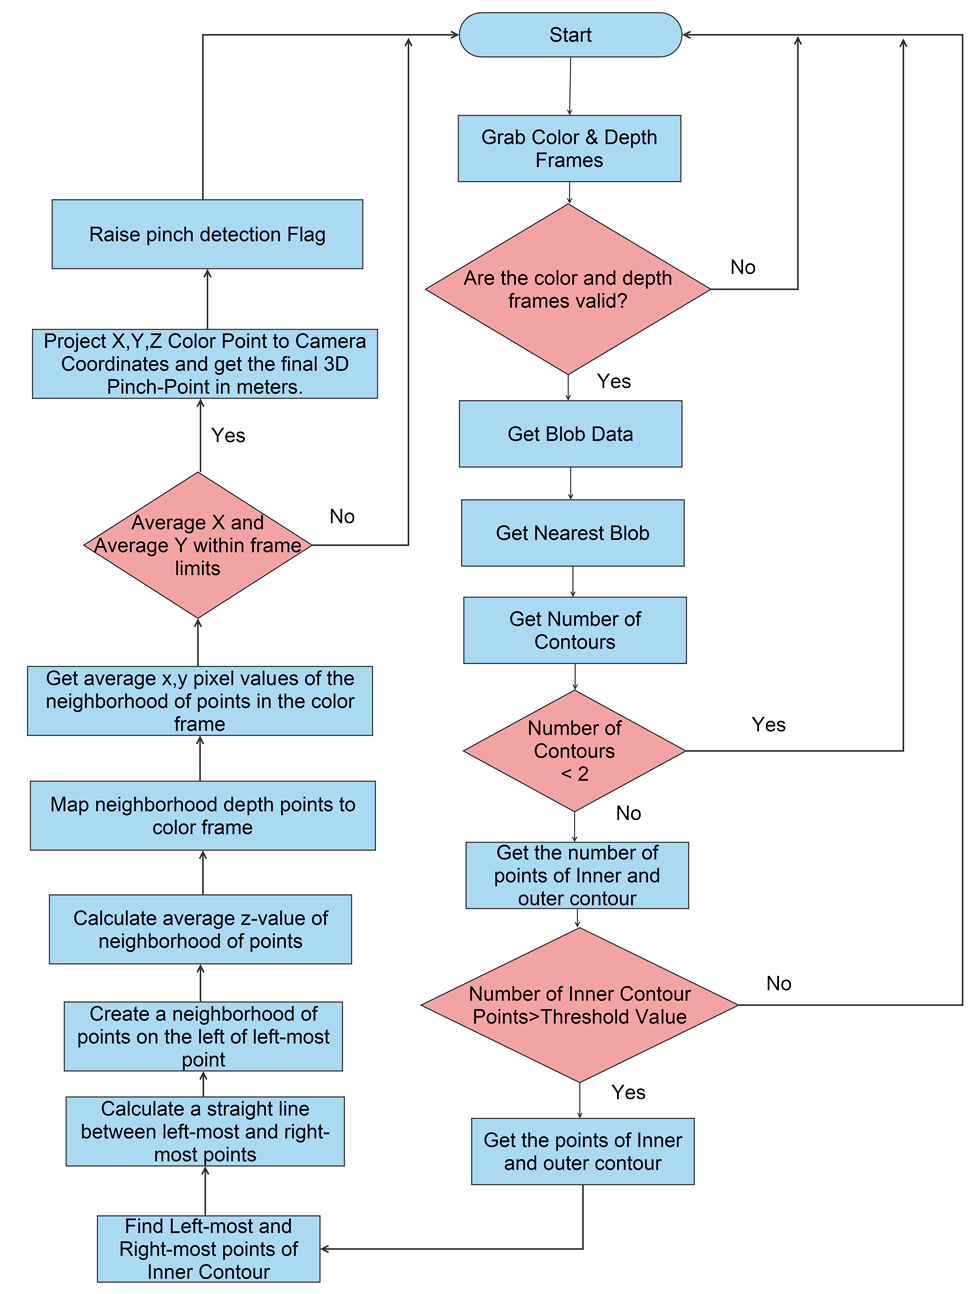
\includegraphics[width=.85\linewidth]{Files/Figures/pinch_gesture_detection.png}
    \caption[Διάγραμμα του αλγορίθμου ανίχνευσης χειρονομίας "τσιμπήματος"]{Διάγραμμα του αλγορίθμου ανίχνευσης χειρονομίας "τσιμπήματος"}
    \label{fig:gesture_rec}
\end{figure}



\begin{figure}[H]
    \centering
    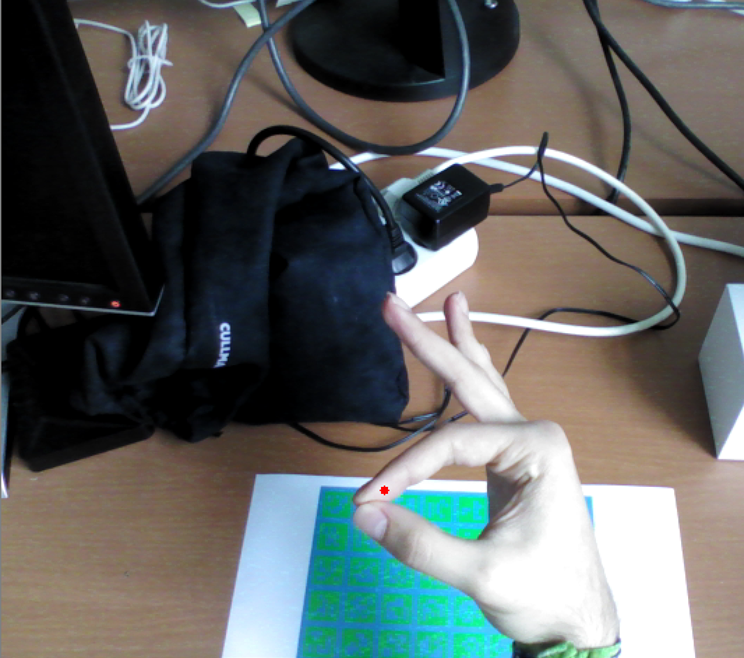
\includegraphics[width=0.45\textwidth]{Files/Figures/pinch.png}
    \caption[Στιγμιότυπο αποτελέσματος αναγνώρισης χειρονομίας "τσιμπήματος"]{Στιγμιότυπο αποτελέσματος αναγνώρισης χειρονομίας "τσιμπήματος"}
    \label{fig:pinch results}
\end{figure}






%ΠΩΣ ΑΝΙΧΝΕΥΕΤΑΙ Η 3D ΘΕΣΗ ΤΣΙΜΠΗΜΑΤΟΣ ΜΕ ΒΑΣΗ ΤΗ ΜΕΘΟΔΟΛΟΓΙΑ ΜΟΥ


Μία σημαντική συνεισφορά της παρούσας διπλωματικής εργασίας αφορά τη μεθοδολογία που παρουσιάζεται σε αυτή την ενότητα, σχετικά με τον εντοπισμό της θέσης όπου λαμβάνει χώρα μία χειρονομία "τσιμπήματος" για συστήματα αλληλεπίδρασης επαυξημένης πραγματικότητας. Στόχος μας είναι να δημιουργηθεί ένα σύστημα αναγνώρισης χειρονομιών για την τρισδιάστατη αλληλεπίδραση και το χειρισμό των εικονικών αντικειμένων. Κάτι τέτοιο πραγματοποιείται χωρίς να χρειάζονται πολύπλοκες διαδικασίες ανάλυσης της κίνησης των δακτύλων ή του χεριού. Αντίθετα, αξιοποιούνται απλές τεχνικές επεξεργασίας εικόνας και υπολογιστικής όρασης.


Στην προηγούμενη ενότητα, παρουσιάστηκε ένας τρόπος ανίχνευσης της χειρονομίας "τσιμπήματος", ωστόσο αυτό μόνο δεν αρκεί για την μετακίνηση των πιονιών του σκακιού στην εφαρμογή που θέλουμε να αναπτύξουμε. Πρέπει να βρούμε το σημείο στο οποίο συνέβη η χειρονομία στο 3D χώρο, με όσο μεγαλύτερη ακρίβεια γίνεται. 



Αν κατά το στάδιο της ανίχνευσης μιας χειρονομίας "τσιμπήματος" διαπιστώθεί ότι έχουμε όντως μία τέτοια χειρονομία, δηλαδή ο αριθμός των περιγραμμάτων του blob είναι μεγαλύτερος ή ίσος του 2 και ο αριθμός των σημείων του εσωτερικού περιγράμματος είναι μεγαλύτερος από μία τιμή κατωφλίου, μπορούμε να συνεχίσουμε για να βρούμε τη θέση στην οποία πραγματοποιήθηκε η χειρονομία ως προς την κάμερα.

Για να συμβεί αυτό, αρχικά επιλέγεται το σημείο του εσωτερικού περιγράμματος που βρίσκεται όσο γίνεται πιο αριστερά, όσον αφορά την εικόνα blob, καθώς και το σημείο του εσωτερικού περιγράμματος που βρίσκεται όσο γίνεται πιο δεξιά. Με βάση αυτά τα 2 σημεία, μπορούμε να βρούμε μία μοναδική ευθεία που ορίζεται από αυτά. Στη συνέχεια, μπορούμε να δημιουργήσουμε μία περιοχή ή καλύτερα μία "γειτονιά"  ενός παραμετρικού αριθμού σημείων, που ανήκουν στη συγκεκριμένη ευθεία που υπολογίστηκε και βρίσκονται αριστερά από το πιο αριστερό σημείο του εσωτερικού περιγράμματος.  Ο αριθμός των σημείων που μπορούμε να πάρουμε μπορεί να οριστεί ως παράμετρος στο πρόγραμμά μας. Προφανώς, όσο περισσότερα σημεία επιλέξουμε, τόσο πιο ακριβές θα είναι το αποτέλεσμα, αλλά τόσο πιο αργό θα γίνεται το πρόγραμμα όπως θα διαπιστωθεί στη συνέχεια. 


Μόλις εκτιμηθεί αυτή η "γειτονιά" σημείων στο frame της εικόνας , μπορούμε να υπολογίσουμε τις τιμές βάθους για καθένα από αυτά τα σημεία και επομένως να εκτιμήσουμε τη μέση τιμή βάθους των εικονοστοιχείων της "γειτονιάς" τα οποία έχουν έγκυρες τιμές. Αυτή η μέση τιμή βάθους, μπορεί να χρησιμποιηθεί αργότερα ως η τιμή βάθους στην οποία πραγματοποιείται η χειρονομία "τσιμπήματος" στον τρισδιάστατο χώρο της σκηνής. 

Αξιοποιώντας, τη δομή UVMap, στην οποία αναφερθήκαμε στην οποια αναφερθήκαμε προηγουμένως, μπορούμε να αντιστοιχίσουμε κάθε σημείο, δηλαδή κάθε εικονοστοιχείο της "γειτονιάς" σημείων στην εικόνα χρώματος που καταγράφει ο αισθητήρας στο ίδιο frame. Υπολογίζουμε τη μέση τιμή των συντεταγμένων εικόνας στην οποία βρίσκεται κάθε σημείο και έχει έγκυρες τιμές (αφού κατά την αντιστοίχιση μπορεί να έχουμε λανθασμένες προσεγγίσεις). Ωστόσο οι τιμές αυτές μετρώνται σε pixels ενώ εμείς θέλουμε να βρούμε το σημείο στο οποίο έλαβε χώρα η χειρονομία στο 3D χώρο σε μονάδες του πραγματικού κόσμου (π.χ μέτρα). Επομένως, πρέπει να προβάλλουμε αυτά τα εικονοστοιχεία χρώματος στο σύστημα συντεταγμένων της κάμερας ώστε να πάρουμε τις αποστάσεις σε μονάδες του πραγματικού κόσμου, δηλαδή στην περίπτωσή μας σε μέτρα. Κάτι τέτοιο μπορεί να γίνει εύκολα μέσω του RealSense SDK.


Μόλις ολοκληρωθεί αυτή η διαδικασία, έχουμε τις τιμές των συντεταγμένων $x,y,z$ για ένα συγκεκριμένο σημείο στον τρισδιάστατο χώρο σε μέτρα, το οποίο θεωρούμε ως το σημείο στο οποίο πραγματοποιήθηκε η χειρονομία "τσιμπήματος" από το χρήστη, ή αλλιώς ως το σημείο στον τρισδιάστατο χώρο όπου ο χρήστης αποφάσισε να "τσιμπήσει" κάποιο εικονικό αντικείμενο. Προφανώς, μόλις συμβεί κάτι τέτοιο και αν οι συντεταγμένες έχουν μία έγκυρη τιμή, ενεργοποιείται μία σημεία που υποδηλώνει στο πρόγραμμά μας ότι πραγματοποιήθηκε μία χειρονομία "τσιμπήματος". 

Εν τέλει, έχουμε το σημείο "τσιμπήματος" στον τρισδιάστατο χώρο ως προς τον αισθητήρα χρώματος της συσκευής. Με βάση την μεθοδολογία που αναφέρθηκε, μπορούμε να αναπτύξουμε την εφαρμογή μας και να υλοποιήσουμε τη λογική του βιντεοπαιχνιδιού σκακιού επαυξημένης πραγματικότητας. 




\begin{figure}[H]
\begin{subfigure}{.5\textwidth}
  \centering
  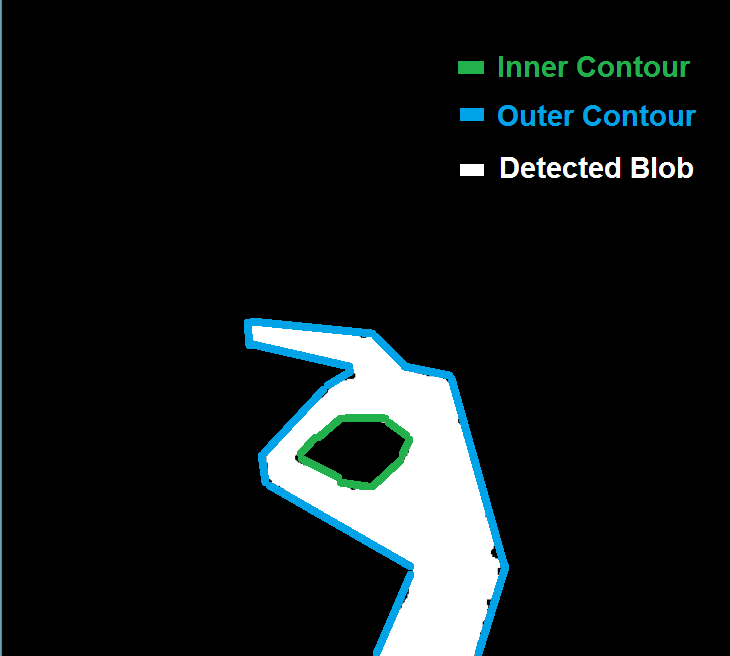
\includegraphics[width=.8\linewidth]{Files/Figures/2.png}
  \caption{1a}
  \label{fig:sfig1}
\end{subfigure}%
\begin{subfigure}{.5\textwidth}
  \centering
  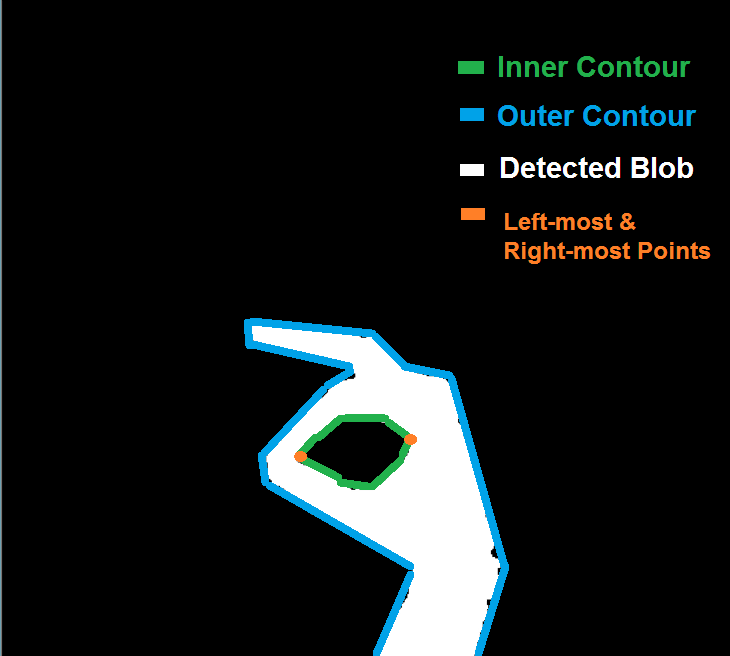
\includegraphics[width=.8\linewidth]{Files/Figures/3.png}
  \caption{1b}
  \label{fig:sfig2}
\end{subfigure}\\
\begin{subfigure}{.5\textwidth}
  \centering
  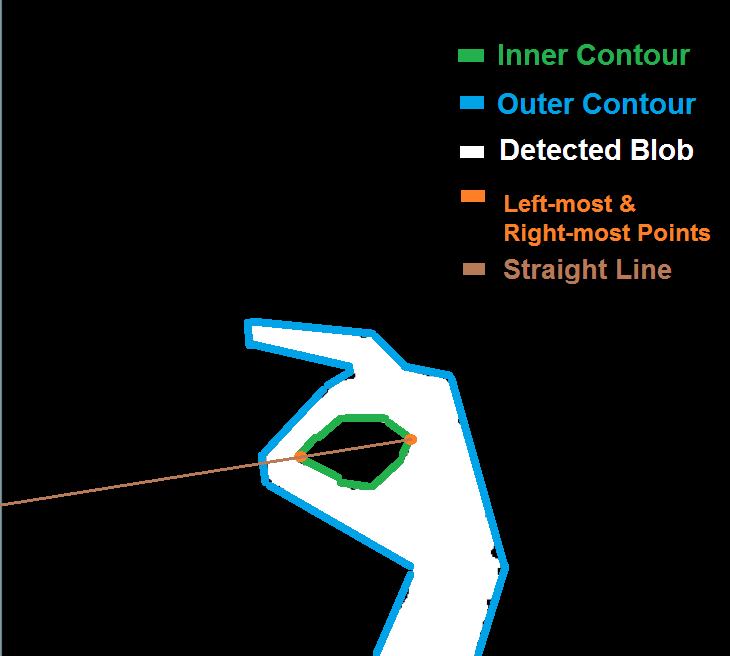
\includegraphics[width=.8\linewidth]{Files/Figures/4.png}
  \caption{1a}
  \label{fig:sfig1}
\end{subfigure}%
\begin{subfigure}{.5\textwidth}
  \centering
  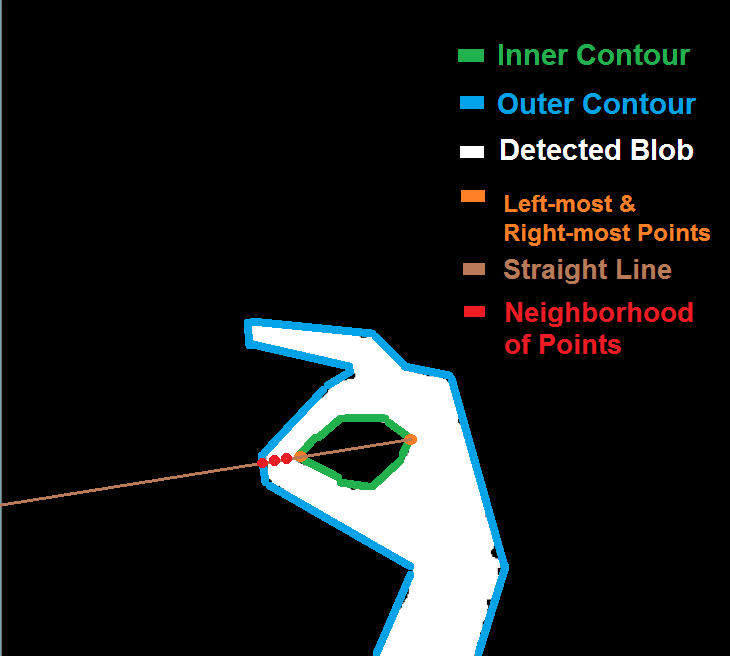
\includegraphics[width=.8\linewidth]{Files/Figures/5.png}
  \caption{1b}
  \label{fig:sfig2}
\end{subfigure}
\caption{Φάσεις εντοπισμού χειρονομίας "τσιμπήματος" στο χώρο}
\label{fig:fig}
\end{figure}



Αφού όλα τα εικονικά αντικείμενα απεικονίζονται ως προς την αρχή των συντεταγμένων του κέντρου της σκακιέρας, δηλαδή του markerboard, η αλληλεπίδραση ανάμεσα στα πραγματικά και τα εικονικά αντικείμενα θα πρέπει να πραγματοποιείται ως προς αυτό το κοινό σύστημα συντεταγμένων. Επομένως, στην επόμενη ενότητα θα παρουσιαστεί η διαδικασία μετατροπής του 3D σημείου όπου πραγματοποιήθηκε η χειρονομία "τσιμπήματος", από το σύστημα συντεταγμένων κάμερας στο σύστημα συντεταγμένων του markerboard.



\section{Tαυτοποίηση Συστημάτων Συντεταγμένων}



Ο μηχανισμός αλληλεπίδρασης που παρουσιάστηκε στις προηγούμενες ενότητες αφορά τη μοντελοποίηση ενός τρόπου επιλογής και χειρισμού εικονικών αντικειμένων που θα μπορούσε κάποιος να παρομοιάσει με το κλικάρισμα ενός ποντικιού και τη μετακίνηση του όπως μετακινούμε ένα εικονίδιο σε μία επιφάνεια εργασίας ενός λειτουργικού συστήματος.


Στη συγκεκριμένη ενότητα, θα παρουσιαστεί η διαδικασία κατά την οποία θα μετατρέψουμε τις συντεταγμένες του σημείου όπου έλαβε χώρα η χειρονομία "τσιμπήματος", ώστε να παρουσιάζονται ως προς το σύστημα συντεταγμένων του markerboard και όχι ως προς το σύστημα συντεταγμένων της κάμερας.


Η ταυτοποίηση των συστημάτων συντεταγμένων βασίζεται στην παραδοχή ότι πρέπει να έχουμε ένα κοινό σύστημα συντεταγμένων τόσο για τα εικονικά αντικείμενα, όσο και για την τοποθεσία της χειρονομίας "τσιμπήματος" μέσω της οποίας αλληλεπιδρά ο χρήστης. Αρχικά πρέπει να βρούμε την πόζα του marker ως προς το σύστημα συντεταγμένων της κάμερας. Αυτό μπορεί να γίνει εύκολα, καθώς η βιβλιοθήκη της ArUco παρέχει τον κατάλληλο μετασχηματισμό από το σύστημα συντεταγμένων του markerboard προς το σύστημα συντεταγμένων της κάμερας.



\begin{equation}
\begin{bmatrix}
x'_{marker} \\ y'_{marker} \\ z'_{marker} \\ 1
\end{bmatrix}
=
\begin{bmatrix}
\mathbf{R} & \mathbf{T}\\ 
0 & 1
\end{bmatrix}
\begin{bmatrix}
x_{marker} \\ y_{marker} \\ z_{marker} \\ 1
\end{bmatrix}
=
^{camera}\mathbf{M}_{marker}
\begin{bmatrix}
x_{marker} \\ y_{marker} \\ z_{marker} \\ 1
\end{bmatrix}
\end{equation}

Στην παραπάνω σχέση, οι μεταβλητές που τονίζονται, σημαίνει ότι έχουν οριστεί ως προς το σύστημα συντεταγμένων της κάμερας.

Έπειτα, καθώς οι συντεταγμένες του σημείου όπου έγινε το "τσίμπημα", είναι γνωστές ως προς την κάμερα, οι ίδιες συντεταγμένες ως προς το markerboard μπορούν να βρεθούν από τη σχέση:


\begin{equation}
\begin{bmatrix}
x_{finger} \\ y_{finger} \\ z_{finger} \\ 1
\end{bmatrix}
=
^{marker}\mathbf{M}_{camera}
\begin{bmatrix}
x'_{finger} \\ y'_{finger} \\ z'_{finger} \\ 1
\end{bmatrix}
=
(^{camera}\mathbf{M}_{marker})^{-1}
\begin{bmatrix}
x'_{finger} \\ y'_{finger} \\ z'_{finger} \\ 1
\end{bmatrix}
\end{equation}


Άρα αρκεί η αντιστροφή του πίνακα που δείχνει τη σχέση των συντεταγμένων κάμερας ως προς το marker και ο πολλαπλασιασμός του με τις συντεταγμένες του σημείου "τσιμπήματος" όπως αυτό ορίστηκε προηγουμένως ως προς την κάμερα. Εν τέλει, έχουμε το σημείο "τσιμπήματος" ως προς το κέντρο του markerboard, κάτι που μας βοηθάει στη συνέχεια της ανάπτυξης της εφαρμογής.


\begin{figure}[H]
    \centering
    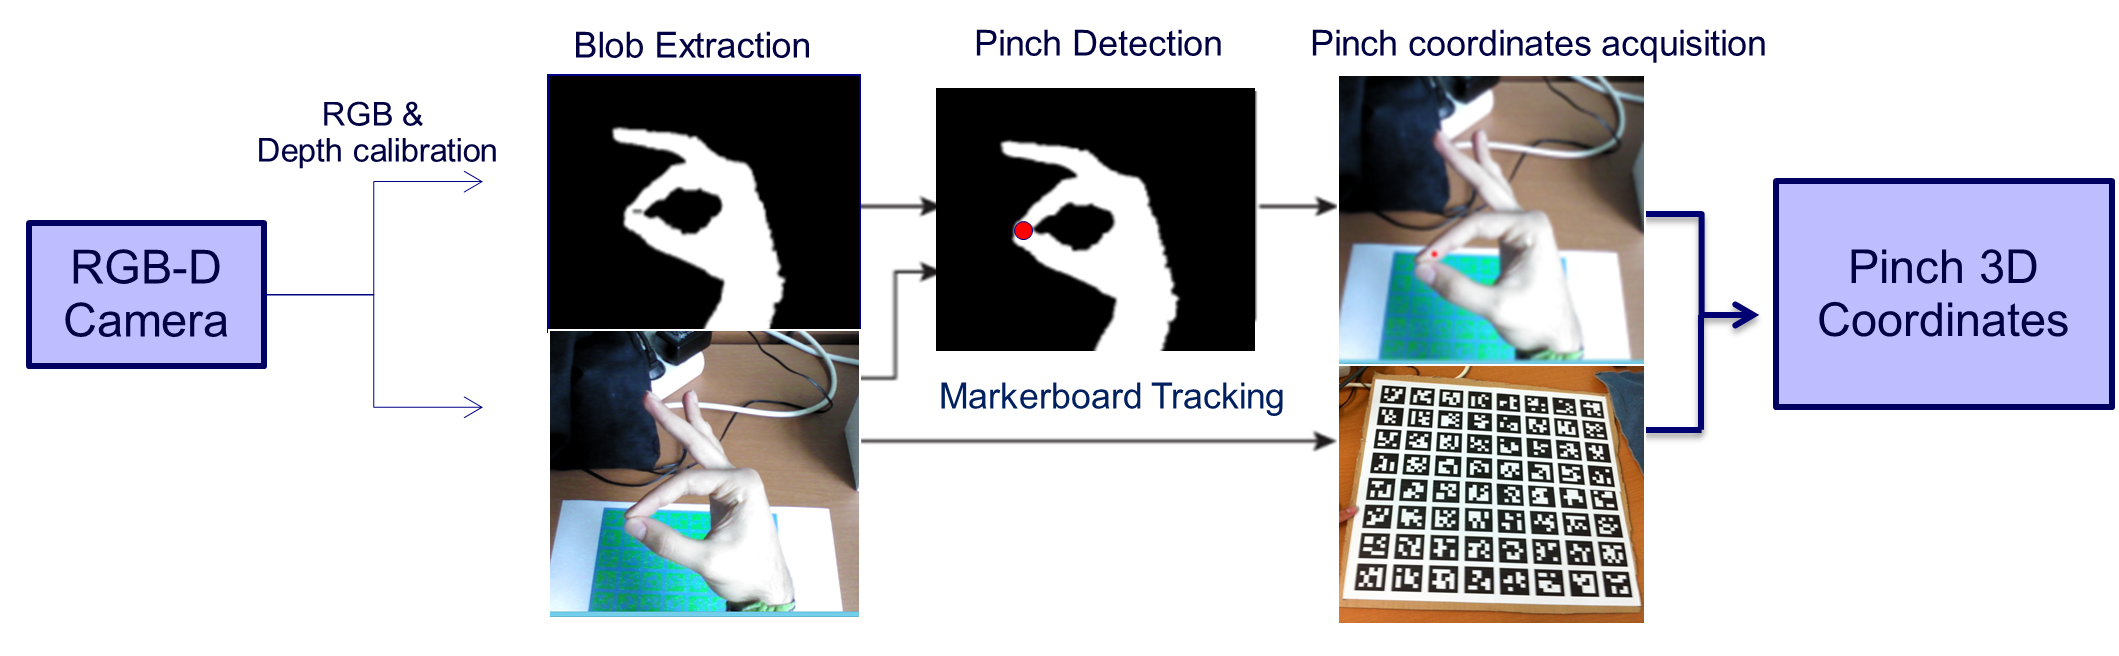
\includegraphics[width=0.9\textwidth]{Files/Figures/procedure.png}
    \caption[Προσέγγιση εντοπισμού σημείου χειρονομίας "τσιμπήματος" ]{Προσέγγιση εντοπισμού σημείου χειρονομίας "τσιμπήματος"}
    \label{fig:procedure}
\end{figure}



Για να δημιουργηθεί ένα σύστημα αλληλεπίδρασης ανθρώπου - υπολογιστή, οι δράσεις που παράγονται όταν λαμβάνει χώρα μία χειρονομία πρέπει να ορίζονται από ένα σύνολο καταστάσεων του συστήματος. Στις επόμενες ενότητες, θα δούμε πώς η δημιουργία τέτοιων καταστάσεων εξυπηρετεί τη λειτουργικότητα της εφαρμογής κατά τη διάρκεια ενός παιχνιδιού σκακιού επαυξημένης πραγματικότητας.





\section{Ενσωμάτωση Μηχανής Σκακιού}

Μετά την υλοποίηση του αλγορίθμου ανίχνευσης της χειρονομίας του "τσιμπήματος" και την αντιμετώπιση του προβλήματος απόκρυψης αντικειμένων, κρίθηκε απαραίτητο, ο χρήστης να μπορεί να παίξει ένα παιχνίδι σκακιού ενάντια στον υπολογιστή. Με αυτό τον τρόπο, πετυχαίνουμε μία φυσική αλληλουχία γεγονότων στο παιχνίδι του σκακιού και προσμοιώνουμε ολοκληρωμένα ένα πραγματικό παιχνίδι σκακιού απέναντι σε έναν αντίπαλο, κάτι που θα μας βοηθήσει στη συνέχεια με την αξιολόγηση του συστήματος. 


Για να μπορέσει ο χρήστης να παίξει σκάκι ενάντια στον υπολογιστή, κανονικά θα έπρεπε να υλοποιηθούν αλγόριθμοι τεχνητής νοημοσύνης που θα επέτρεπαν στο πρόγραμμα μας να καθορίσει την επόμενη κίνηση του υπολογιστή με βάση τις προηγούμενες κινήσεις που έλαβαν μέρος κατά τη διάρκεια του παιχνιδιού. Ωστόσο η υλοποίηση τέτοιων αλγορίθμων για την εφαρμογή μας δεν βρίσκεται μέσα στους σκοπούς της παρούσας διπλωματικής εργασίας και έπρεπε να αναζητηθεί ένα απλός τρόπος για την ενσωμάτωση λειτουργιών τεχνητής νοημοσύνης. 


Εκεί ακριβώς προκύπτει η λύση των μηχανών σκακιού. Μία μηχανή σκακιού δεν είναι τίποτα άλλο από ένα πρόγραμμα υπολογιστή το οποίο δέχεται σαν είσοδο την θέση ενός πιονιού στη σκακιέρα, αναλύει τις θέσεις όλων των πιονιών και υπολογίζει την καλύτερη δυνατή κίνηση με βάση τη διάταξη των πιονιών στη σκακιέρα μέσα σε ένα χρονικό περιθώριο που ορίζεται εκ των προτέρων. Η μηχανή σκακιού μπορεί να εκτιμήσει τις επόμενες κινήσεις, αλλά συνήθως δεν αλληλεπιδρά απευθείας με το χρήστη, καθώς οι περισσότερες μηχανές δεν έχουν δική τους γραφική διεπαφή για την επικοινωνία με το χρήστη. Αντίθετα οι περισσότερες είναι εφαρμογές κονσόλας που επικοινωνούν με μία γραφική διεπαφή μέσω ενός καθορισμένου πρωτοκόλλου. Αυτό επιτρέπει στο χρήστη να παίζει ενάντια σε πολλές διαφορετικές μηχανές χωρίς να χρειάζεται να εκπαιδευτεί εκ νέου σε νέες διεπαφές κάθε φορά και επιτρέπει σε διαφορετικές μηχανές να παίζουν η μία ενάντια στην άλλη. Στη συγκεκριμένη περίπτωση, η εφαρμογή μας παίζει το ρόλο της γραφικής διεπαφής ως τώρα. 


Στις μέρες μας, ο πιο πιο γνωστός τρόπος επικοινωνίας με μηχανές σκακιού πραγματοποιείται μέσω ενός πρωτοκόλλου που ονομάζεται Universal Chess Interface (UCI) Protocol. Πρόκειται για ένα πρωτόκολλο ανοιχτής επικοινωνίας που επιτρέπει σε μία μηχανή σκακιού ενός προγράμματος να επικοινωνεί με τη διεπαφή χρήστη μέσα από ένα σύνολο αυστηρά καθορισμένων εντολών. Επομένως, για να ενσωματώσουμε μία μηχανή σκακιού στην εφαρμογή μας, πρέπει να βρούμε ένα τρόπο ώστε να γίνει ανταλλαγή εντολών (συμβολοσειρές) ανάμεσα στην εφαρμογή μας και τη μηχανή σκακιού. 


Η μηχανή δέχεται εντολές μέσω standard input από μια εφαρμογή και παράγει τις απαντήσεις σε συμβολοσειρές του standard output. Δεν έχει δηλαδή γραφική διεπαφή, είσοδο μέσω ποντικιού ή εικόνες, παρά μόνο ένα απλό παράθυρο κονσόλας, που δεν είναι τίποτα περισσότερο παρά ένα εκτελέσιμο (.exe) αρχείο. 

Προκειμένου να υλοποιηθεί αυτή η επικοινωνία με το εκτελέσιμο αρχείο μιας μηχανής σκακιού αποφασίστηκε να αξιοποιηθεί η δυνατότητα που προσφέρει η βιβλιοθήκη Qt μέσω μιας κλάσης με το όνομα QProcess, η οποία επιτρέπει στο πρόγραμμά μας να εκκινήσει ένα εκτελέσιμο αρχείο, καθώς και να διαβάσει και να γράψει εντολές συμβολοσειρών από και προς αυτό. Η αλληλεπίδραση με τη μηχανή σκακιού ξεκινά με μία εντολή "uci", η οποία επικοινωνεί με τη μηχανή λέγοντας της να ταυτοποιήσει τον εαυτό της, δηλαδή να δώσει σαν έξοδο τα χαρακτηριστικά της όπως την ονομασία της, την έκδοσή της κλπ.  Έπειτα, δέχεται εντολές που μπορούν να αλλάξουν ορισμένες προεπιλεγμένες τιμές ιδιοτήτων που επηρεάζουν τα δεδομένα τα οποία θα προβάλλονται σαν έξοδος από τη μηχανή. Μετέπειτα, η μηχανή δέχεται ως είσοδο από την εφαρμογή μας την κίνηση που πραγματοποίησε ο χρήστης και εξάγει την επόμενη καλύτερη κίνηση που μπορεί να εκτελέσει ο αντίπαλος, δηλαδή ο υπολογιστής.
Η μηχανή σκακιού δέχεται σαν παράμετρο το χρόνο τον οποίο έχει για να υπολογίσει την κίνηση αυτή, ψάχνοντας για την καλύτερη δυνατή κίνηση. Ξεκινά την αναζήτηση και εκτιμά την καλύτερη κίνηση που υπάρχει πριν λήξει το χρονικό περιθώριο που ορίζεται στην αρχή της εκτέλεσης της μηχανής. 

Για την εφαρμογή μας, θεωρήσαμε ότι το χρονικό αυτό περιθώριο πρέπει να είναι ιδιαίτερα μικρό (40ms), ώστε να μην "παγώνει" η απεικόνιση των εικονικών αντικειμένων και να μπορούμε να παίρνουμε άμεσα feedback από το πρόγραμμα. Συνήθως οι μηχανές σκακιού δεν έχουν τη δυνατότητα να αντιλαμβάνονται αν μία εντολή κίνησης που δίνεται από το χρήστη είναι έγκυρη ή όχι, με βάση τον τύπο των πιονιών και την κατάσταση της σκακιέρας. Για το λόγο αυτό επιλέχθηκε να χρησιμοποιηθεί η μηχανή iCE \cite{ice}, η οποία ελέγχει αν η κίνηση που γίνεται είναι επιτρεπτή ή όχι. Αν η κίνηση δεν επιτρέπεται, τότε η μηχανή επιστρέφει ως έξοδο τη συμβολοσειρά "Invalid chess move". Αυτή η ιδιότητα επιτρέπει την υλοποίηση μιας αρχιτεκτονικής στον κώδικά μας, η οποία δε θα είναι επιρρεπής σε λανθασμένες κινήσεις όταν αυτές γίνονται κατά λάθος από το χρήστη. Επιπλέον, η μηχανή που χρησιμοποιήθηκε μπορεί να ανιχνεύσει αν το παιχνίδι ολοκληρώθηκε και ποιος είναι νικητής ώστε να μπορούμε να ενημερώσουμε το χρήστη για το αποτέλεσμα του παιχνιδιού. 

Συμπερασματικά, υλοποίησαμε τη βασική λειτουργικότητα για την αποστολή και λήψη συμβολοσειρών προς και από τη μηχανή σκακιού και με βάση αυτές τις συμβολοσειρές το πρόγραμμά μας εκτελεί συγκεκριμένες δράσεις.






\section{Χειρισμός και Απεικόνιση Εικονικών Αντικειμένων} \label{s:rendering}



Πλέον γνωρίζουμε πότε ο χρήστης πραγματοποιεί μία χειρονομία "τσιμπήματος", τη θέση του "τσιμπήματος" στον τρισδιάστατο χώρο ως προς το markerboard και πώς μπορούμε να ενσωματώσουμε μία μηχανή σκακιού για την αξιοποίηση μεθόδων τεχνητής νοημοσύνης, ώστε ο χρήστης να μπορεί να παίξει με αντίπαλο τον υπολογιστή.
Επομένως, μπορούμε να υλοποιήσουμε τη λογική του βιντεοπαιχνιδιού ενός σκακιού επαυξημένης πραγματικότητας, με στόχο τη σωστή απεικόνιση και τον χειρισμό των εικονικών αντικειμένων.


Όπως είναι ευρύτερα γνωστό, κατά τη διάρκεια ενός παιχνιδιού σκακιού πραγματοποιούνται διαδοχικές κινήσεις από τους 2 παίκτες. Ένας παίκτης μπορεί να μετακινήσει ένα πιόνι με βάση τον τύπο του και τις ιδιότητές του, που του επιτρέπουν να κινηθεί σε συγκεκριμένα τετράγωνα της σκακιέρας ή να αιχμαλωτίσει ένα αντίπαλο πιόνι και να τοποθετηθεί στο τετράγωνο εκείνο. Επιπλέον υπάρχουν ορισμένες ειδικές κινήσεις όπως το ροκέ, όπου πραγματοποιείται μετακίνηση του βασιλιά δύο τετράγωνα προς τον πύργο και μετακίνηση του πύργου στο τετράγωνο ανάμεσα στην αρχική και τελική θέση του βασιλιά. Είναι η μοναδική κίνηση στο σκάκι, που κάποιος παίκτης μπορεί να μετακινήσει στη σειρά του, ταυτόχρονα δύο πιόνια.

Πιο συγκεκριμένα, όταν ένας χρήστης επιχειρήσει μία χειρονομία "τσιμπήματος" με στόχο να μετακινήσει ένα πιόνι, πρέπει το πιόνι να απεικονίζεται ως προς το σημείο όπου πραγματοποιήθηκε η χειρονομία ώστε να κινείται όπως κινείται και το χέρι του χρήστη.
Αν ο χρήστης αποφασίσει να ολοκληρώσει μία κίνηση, πρέπει να μετακινήσει το πιόνι πάνω από ένα άλλο τετράγωνο της σκακιέρας και να πραγματοποιήσει μία κίνηση αντίθετη της χειρονομίας "τσιμπήματος" που υποδεικνύει απελευθέρωση του αντικειμένου (pinch-out). Η κίνηση αυτή πραγματοποιείται όταν ο δείκτης και ο αντίχειρας παύουν να αγγίζουν ο ένας τον άλλον.  
Μόλις η κίνηση αυτή πραγματοποιηθεί και αν είναι έγκυρη, πρέπει το σύστημα να απευθυνθεί στη μηχανή σκακιού και να μάθει την καλύτερη κίνηση που προτείνεται για τον αντίπαλο μέσω των αλγορίθμων τεχνητής νοημοσύνης. 
Μόλις η μηχανή απαντήσει, έχουμε ουσιαστικά μία κίνηση που πρέπει να πραγματοποιηθεί από τα αντίπαλα πιόνια και επομένως πρέπει να ανανεωθεί η σκακιέρα και η θέση των πιονιών πάνω σε αυτή. 

Αυτή η αλληλουχία γεγονότων που αναφέρθηκε είναι αρκετά πολύπλοκο να υλοποιηθεί απευθείας, επομένως αποφασίστηκε να εκτελούνται διαφορετικές εντολές με βάση την κατάσταση του παιχνιδιού σε κάθε χρονική στιγμή και το αν έχει ανιχνευθεί μία χειρονομία "τσιμπήματος".

Συγκεκριμένα, όταν ενεργοποιείται μία "σημαία" που υποδεικνύει ότι ανιχνεύθηκε ένα "τσίμπημα" σε κάθε frame, πρέπει να αλλάζει η κατάσταση του συστήματος λαμβάνοντας υπόψη ορισμένες παραμέτρους.

Υπάρχουν 5 βασικές καταστάσεις στην υλοποίηση που προτείνεται με τις ονομασίες Free, Pinch-In, Pinch-Continuous, Pinch-Out και enemy-Move. 

Όπως φαίνεται και από το διάγραμμα~\ref{fig:states}, η κατάσταση του συστήματος αλλάζει με βάση την προηγούμενη κατάσταση του προγράμματος και συγκεκριμένες παραμέτρους. Αφού έγινε ανάλυση της κίνησης ενός παίκτη προσεκτικά, υλοποιήθηκαν οι καταστάσεις που περιγράφονται αναλυτικά παρακάτω:

\begin{enumerate}
\item \textbf{FREE}: Ο χρήστης δεν πραγματοποιεί καμία χειρονομία ή το σύστημα δεν μπορεί να εντοπίσει καμία χειρονομία τσιμπήματος στο συγκεκριμένο frame.

\item \textbf{PINCH-IN}: Ανιχνεύθηκε μία χειρονομία τσιμπήματος και επομένως, αν η προηγούμενη κατάσταση του συστήματος είναι η FREE, η παρούσα κατάσταση μετατρέπεται σε PINCH-IN.


\item \textbf{PINCH-CONTINUOUS}: Ανιχνεύθηκε μία χειρονομία τσιμπήματος και αν η προηγούμενη κατάσταση του συστήματος είναι η PINCH-IN, η παρούσα κατάσταση μετατρέπεται σε PINCH-CONTINUOUS. Αυτό σημαίνει ότι ο χρήστης μπορεί να θέλει να μετακινήσει ένα εικονικό πιόνι. 

\item \textbf{PINCH-OUT}: Δεν υπάρχει ανίχνευση χειρονομίας τσιμπήματος για έναν συγκεκριμένο αριθμό διαδοχικών frames. Η προηγούμενη κατάσταση είναι είτε Pinch-In ή Pinch-Continuous, επομένως μπορεί να έχουμε μία ολοκληρωμένη κίνηση από το χρήστη. 


\item \textbf{ENEMY-MOVE}: Το σύστημα εισέρχεται σε αυτή την κατάσταση μετά από κάθε κατάσταση PINCH-OUT και αν η κίνηση είναι που πραγματοποιήθηκε θεωρείται έγκυρη. Επίσης το σύστημα παραμένει σε αυτή την κατάσταση όσο διαρκεί το animation της κίνησης του πιονιού του αντιπάλου, δηλαδή του υπολογιστή. 
\end{enumerate}




\begin{figure}[H]
    \centering
    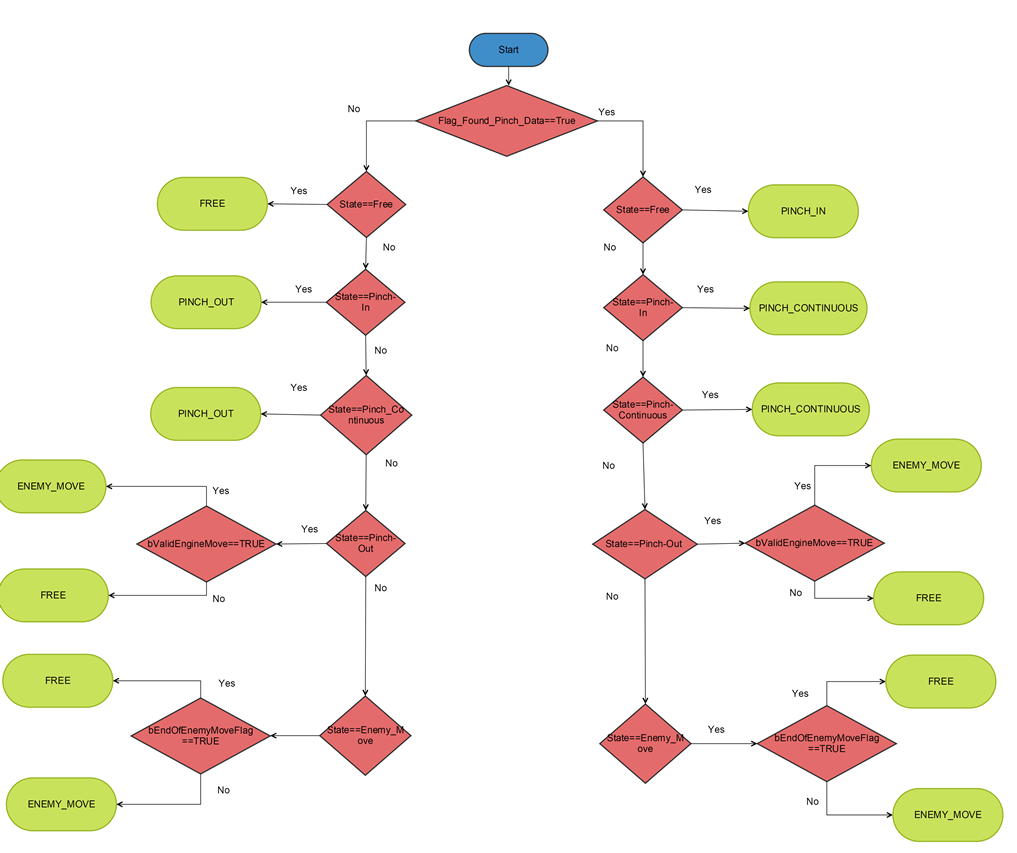
\includegraphics[width=0.95\textwidth]{Files/Figures/change_of_states.png}
    \caption[Διάγραμμα του αλγορίθμου αλλαγής καταστάσεων της εφαρμογής]{Διάγραμμα του αλγορίθμου αλλαγής καταστάσεων της εφαρμογής}
    \label{fig:states}
\end{figure}






Αφού το σύστημα εισέλθει σε μία συγκεκριμένη κατάσταση, μπορούμε στη συνέχεια να εκτελέσουμε εντολές με τις οποίες τα εικονικά πιόνια θα απεικονιστούν ή όχι. Το κομμάτι αυτό είναι ιδιαίτερα σημαντικό, καθώς για παράδειγμα, όταν ένα πιόνι αιχμαλωτίζει ένα άλλο, τότε αυτό πρέπει να σταματήσει να απεικονίζεται στη σκακιέρα.


Συγκεκριμένα, αν η τρέχουσα κατάσταση του συστήματος είναι η Free, τότε χρειάζεται να απεικονίσουμε κάθε εικονικό πιόνι που υπάρχει στην εσωτερική αναπαράσταση της σκακιέρας, δηλαδή σε μία δομή δεδομένων που αποτελείται από ένα πίνακα με δείκτες προς μεταβλητές που προσομοιώνουν τα πιόνια και τις ιδιότητές τους. Με βάση τον τύπο κάθε πιονιού, μπορούμε να απεικονίσουμε το σωστό 3D μοντέλο (π.χ βασίλισσα, αξιωματικός κ.λπ) πάνω από το κατάλληλο τετράγωνο της σκακιέρας. 


\begin{figure}[H]
    \centering
    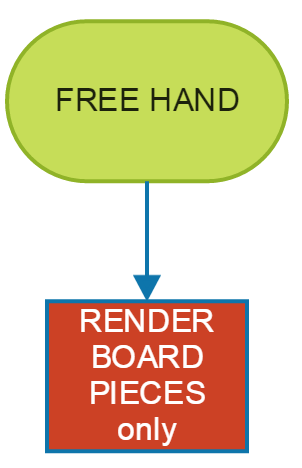
\includegraphics[scale=0.35, angle=0]{Files/Figures/free_hand.png}
    \caption[Διάγραμμα ροής κατάστασης Free]{[Διάγραμμα ροής κατάστασης Free}
    \label{fig:free}
\end{figure}



Όταν η τρέχουσα κατάσταση είναι η Pinch-In, τότε ο χρήστης μπορεί να θέλει να επιλέξει ένα πιόνι. Ωστόσο πρέπει με ακρίβεια να εντοπίσουμε ποιο πιόνι είναι αυτό το οποίο προσπαθεί να επιλέξει ο χρήστης από όλα αυτά που υπάρχουν στη σκακιέρα σε κάθε χρονική στιγμή. 

Για να συμβεί αυτό, ακολουθείται μία διαδικασία κατά την οποία, με βάση την θέση στην οποία συνέβη το "τσίμπημα" στον τρισδιάστατο χώρο, υπολογίζουμε όλες τις ευκλείδιες αποστάσεις από αυτή και το κέντρο όλων των τετραγώνων της σκακιέρας, τα οποία έχουν ένα πιόνι επάνω τους και αυτό το πιόνι ανήκει στο χρήστη και όχι στον υπολογιστή. Από το σύνολο των τιμών αυτών των αποστάσεων, βρίσκουμε το τετράγωνο εκείνο το οποίο απέχει λιγότερο από το σημείο "τσιμπήματος", καθώς και την τιμή της απόστασης σε μέτρα. 


%δες jimemenez selida 20!!!
Ωστόσο, για να αποτραπεί η επιλογή ενός πιονιού, όταν η χειρονομία του χρήστη γίνεται αρκετά μακριά από τα εικονικά πιόνια ή ακόμα και εκτός της σκακιέρας, χρειάζεται να ικανοποιείται μία συνθήκη, ώστε η απόσταση αυτή η οποία ορίστηκε ως μικρότερη, να είναι και μικρότερη από μία τιμή, η οποία εκτιμήθηκε μετά από δοκιμές.


Αν η επιλογή του πιονιού θεωρηθεί από τον αλγόριθμο αυτό ως έγκυρη, τότε κατά τη διαδικασία του σχεδιασμού των πιονιών μέσω της OpenGL, θα απεικονίσουμε όλα τα πιόνια της σκακιέρας, εκτός από αυτό που επιλέχθηκε. Αυτό το οποίο επιλέχθηκε, αντίθετα, θα απεικονιστεί στην επαυξημένη σκηνή, αλλά όχι στατικό πάνω από το τετράγωνο, αλλά στη θέση όπου έγινε η χειρονομία "τσιμπήματος" του χρήστη. Σε αντίθετη περίπτωση, δεν έχουμε έγκυρη επιλογή πιονιού, επειδή ο χρήστης προσπάθησε να επιλέξει ένα πιόνι πιο μακριά από ότι έπρεπε στη σκακιέρα και επομένως απεικονίζονται στην επαυξημένη σκηνή όλα τα πιόνια τα οποία βρίσκονται στη σκακιέρα την τρέχουσα χρονική στιγμή (όσα δεν έχουν αιχμαλωτιστεί κλπ).




\begin{figure}[H]
    \centering
    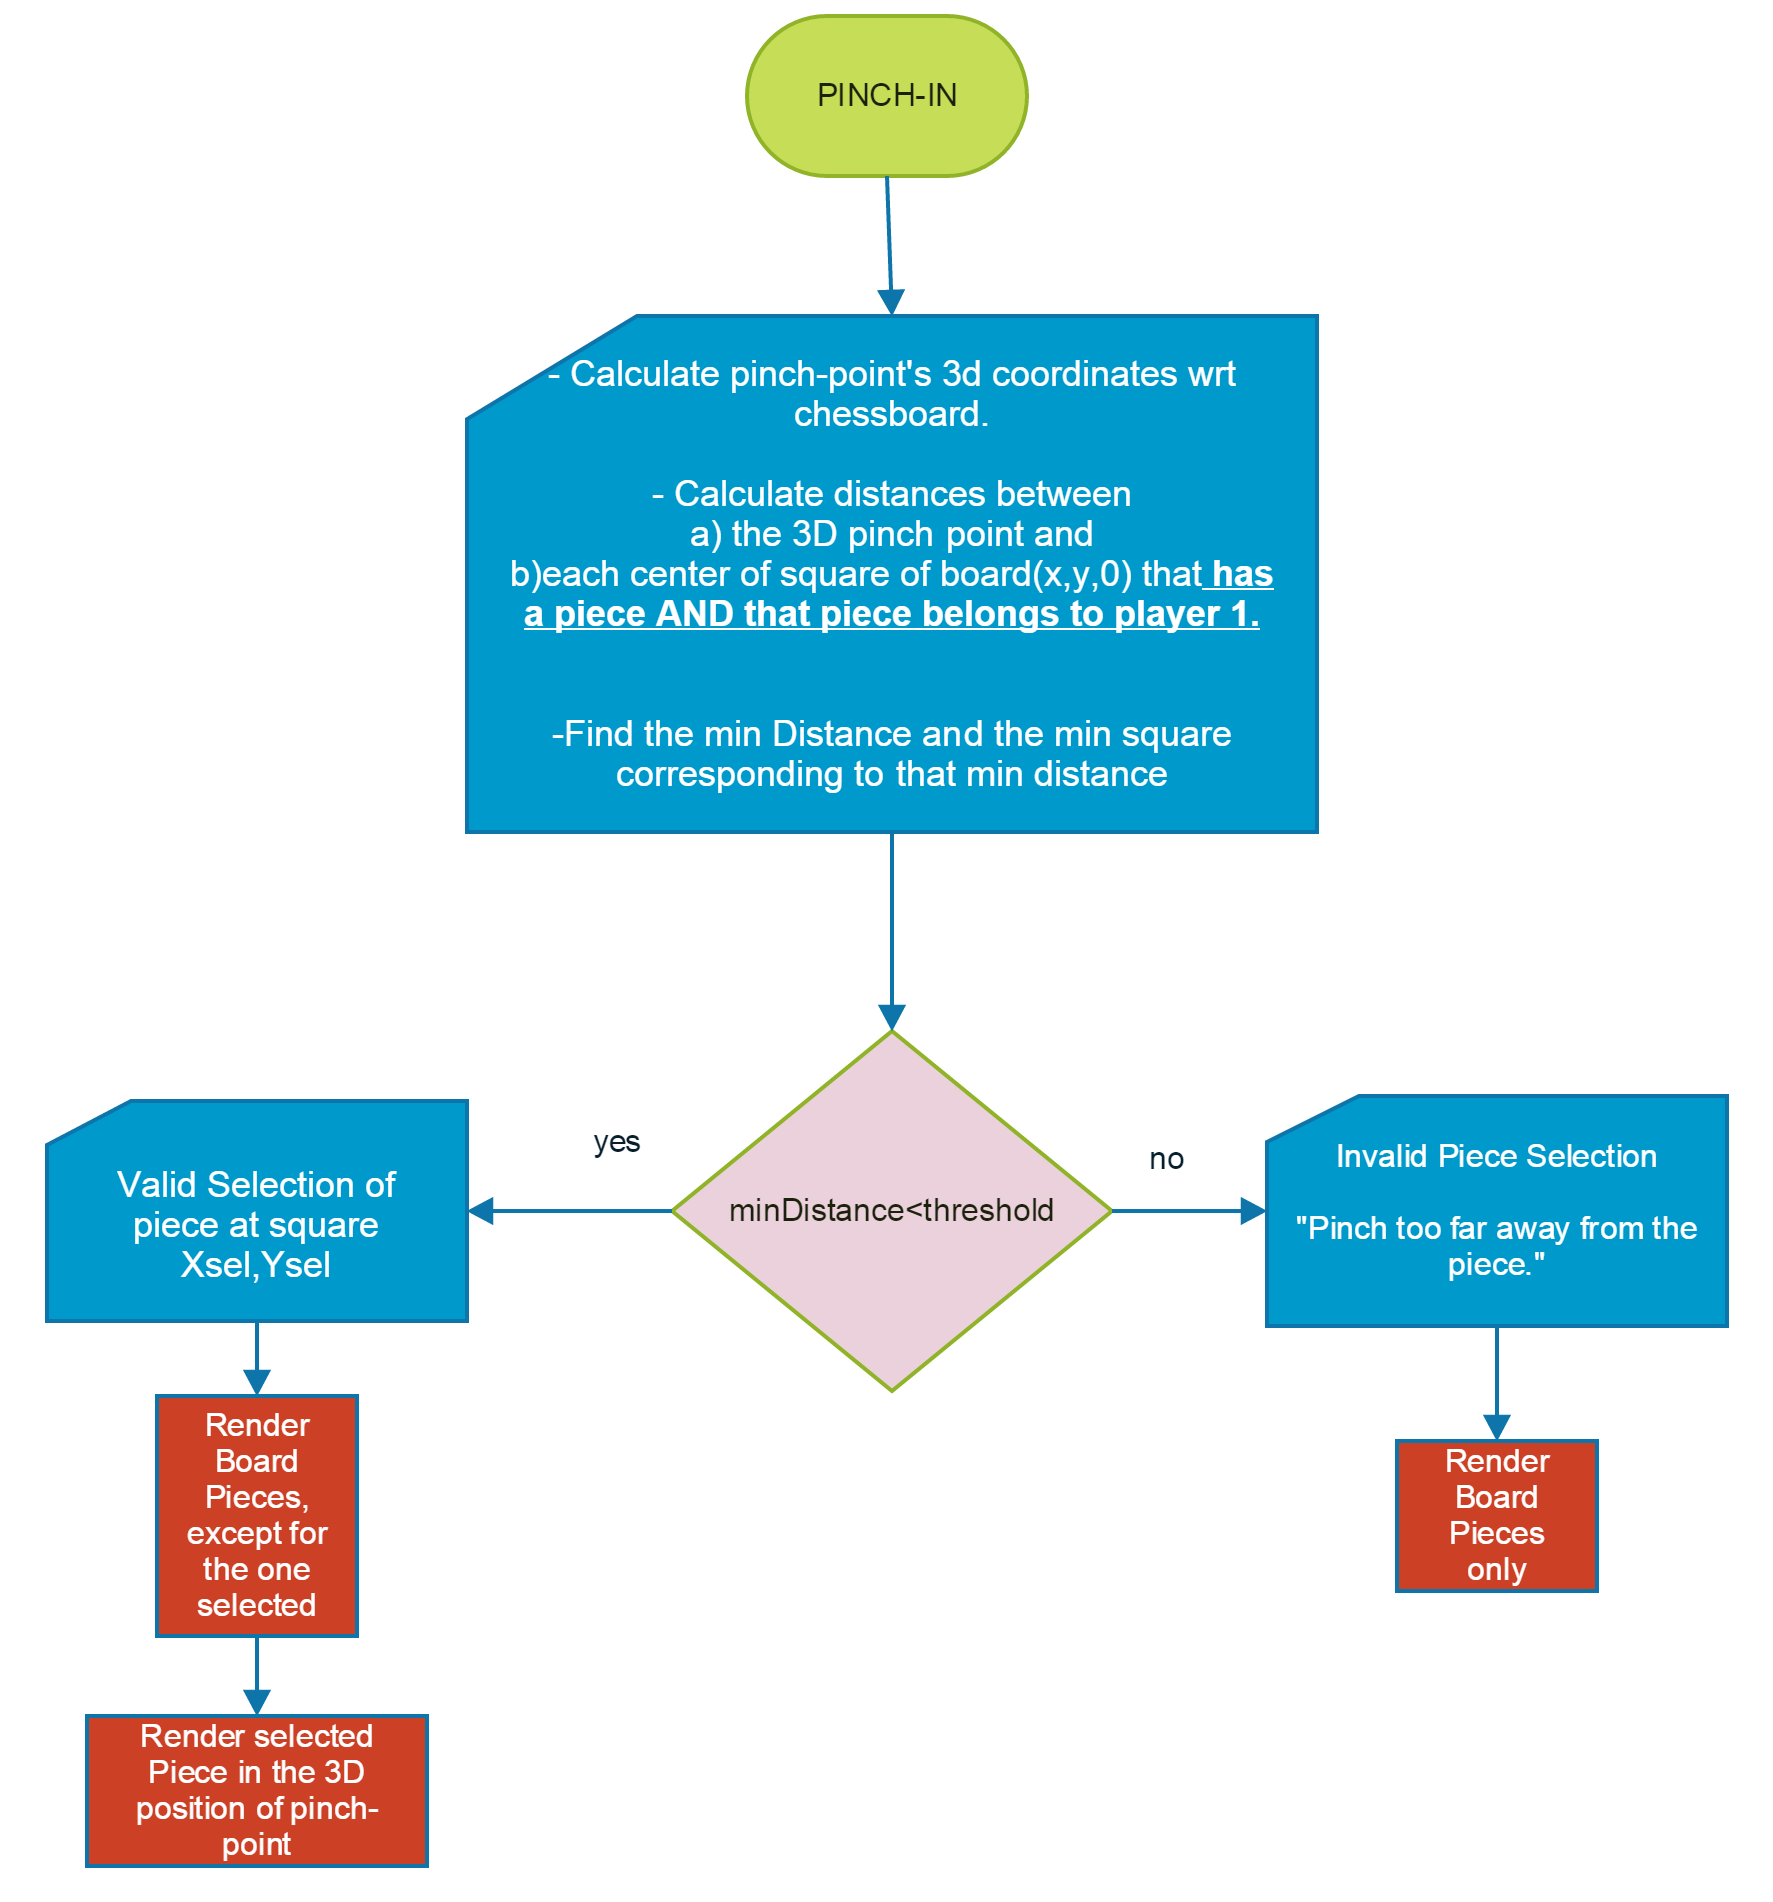
\includegraphics[width=0.86\textwidth]{Files/Figures/pinch_in.png}
    \caption[Διάγραμμα ροής κατάστασης Pinch-In]{Διάγραμμα ροής κατάστασης Pinch-In}
    \label{fig:pinch-in}
\end{figure}


Όταν η κατάσταση του συστήματος είναι η Pinch-Continuous, τότε αν στην προηγούμενη κατάσταση είχαμε έγκυρη επιλογή ενός πιονιού, θα απεικονιστούν όλα τα πιόνια της σκακιέρας, εκτός από αυτό που επιλέχθηκε, το οποίο θα απεικονιστεί ως προς το σημείο "τσιμπήματος". 

\begin{figure}[H]
    \centering
    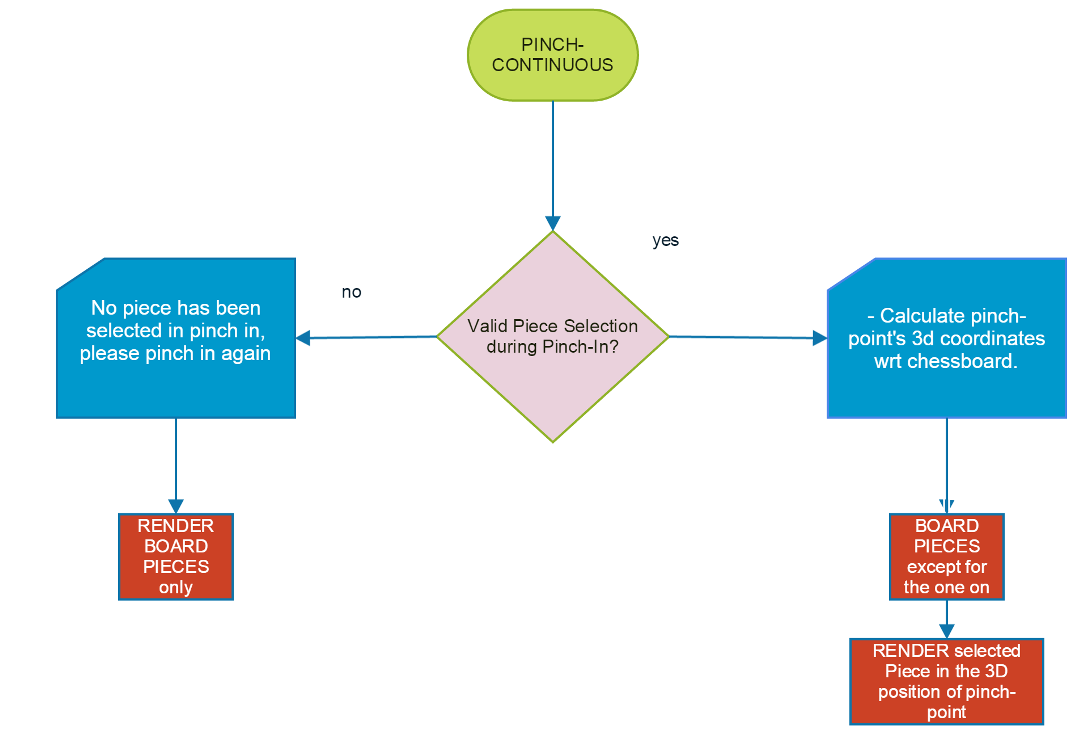
\includegraphics[width=0.95\textwidth]{Files/Figures/pinch_continuous_state.png}
    \caption[Διάγραμμα ροής κατάστασης Pinch-Continuous]{Διάγραμμα ροής κατάστασης Pinch-Continuous}
    \label{fig:pinch-continuous}
\end{figure}



Αφού διαπιστωθεί αν επιλέχθηκε έγκυρα ένα πιόνι στις προηγούμενες καταστάσεις, στην κατάσταση Pinch-Out πρέπει να βρεθεί το σημείο εκείνο στη σκακιέρα όπου ο χρήστης επέλεξε να αφήσει το πιόνι το οποίο μετακινεί. Το πιόνι αυτό, έπειτα, πρέπει να ανατεθεί στο νέο τετράγωνο της σκακιέρας και να ανανεωθεί η δομή της σκακιέρας και η διάταξη των πιονιών.

Για να πραγματοποιηθεί αυτή η διαδικασία, πρέπει αρχικά να υπολογιστούν οι αποστάσεις ανάμεσα στην προβολή του τελευταίου σημείου "τσιμπήματος" που ανιχνεύθηκε πριν απελευθερώσει ο χρήστης τον αντίχειρα και το δείκτη του και το κέντρο κάθε τετραγώνου της σκακιέρας, όπου υπάρχει αντίπαλο πιόνι ή ελεύθερο τετράγωνο. Στη συνέχεια, παίρνουμε τις συντεταγμένες του τετραγώνου που βρίσκεται πιο κοντά στην προβολή του σημείου "τσιμπήματος". Το συγκεκριμένο τετράγωνο θα θεωρηθεί ως το τετράγωνο τελικής θέσης του πιονιού. 


Μόλις επιλεγεί το συγκεκριμένο τετράγωνο, ουσιαστικά έχουμε μία ολοκληρωμένη κίνηση που προσπαθεί να πραγματοποιήσει ο χρήστης. Ωστόσο, αυτή η κίνηση μπορεί να μην είναι έγκυρη με βάση τους κανόνες που ισχύουν στο σκάκι. Για παράδειγμα ο χρήστης μπορεί να προσπαθήσει να μετακινήσει τον βασιλιά 3 ή περισσότερα τετράγωνα μακριά από την αρχική του θέση. Για να αντιμετωπιστεί το συγκεκριμένο πρόβλημα, πρέπει να γίνεται έλεγχος της εγκυρότητας κάθε κίνησης μέσω της μηχανής σκακιού που χρησιμοποιείται (iCE Engine). 


Πιο συγκεκριμένα, πρέπει αρχικά να μετασχηματίσουμε την κίνηση που πραγματοποίησε ο χρήστης στη σκακιέρα και η οποία αναπαρίσταται από 4 αριθμούς που δείχνουν τις αρχικές και τις τελικές συντεταγμένες του τετραγώνου στο 8 x 8 πλέγμα της σκακιέρας σε μία συμβολοσειρά που είναι συμβατή με το πρωτόκολλο UCI (π.χ ο αριθμός 0102 γίνεται A2A3). Με αυτόν τον τρόπο παίρνουμε μία απάντηση από τη μηχανή σχετικά με το αν η κίνηση του χρήστη είναι έγκυρη ή όχι. 


Αν η κίνηση δεν είναι έγκυρη, τότε δε χρειάζεται να ανανεωθεί η εσωτερική αναπαράσταση της διάταξης των πιονιών στη σκακιέρα και το πιόνι που έγινε προσπάθεια να μετακινηθεί, επιστρέφει πίσω στην αρχική του θέση. Διαφορετικά, έχουμε μία έγκυρη κίνηση, πηγαίνουμε στην επόμενη κατάσταση που είναι η Enemy-Move και ανανεώνεται η θέση του πιονιού που κινείται στην εσωτερική αναπαράσταση της διάταξης των πιονιών. Τέλος απεικονίζονται στην οθόνη, όλα τα πιόνια που ανήκουν στη σκακιέρα.


\begin{figure}[H]
    \centering
    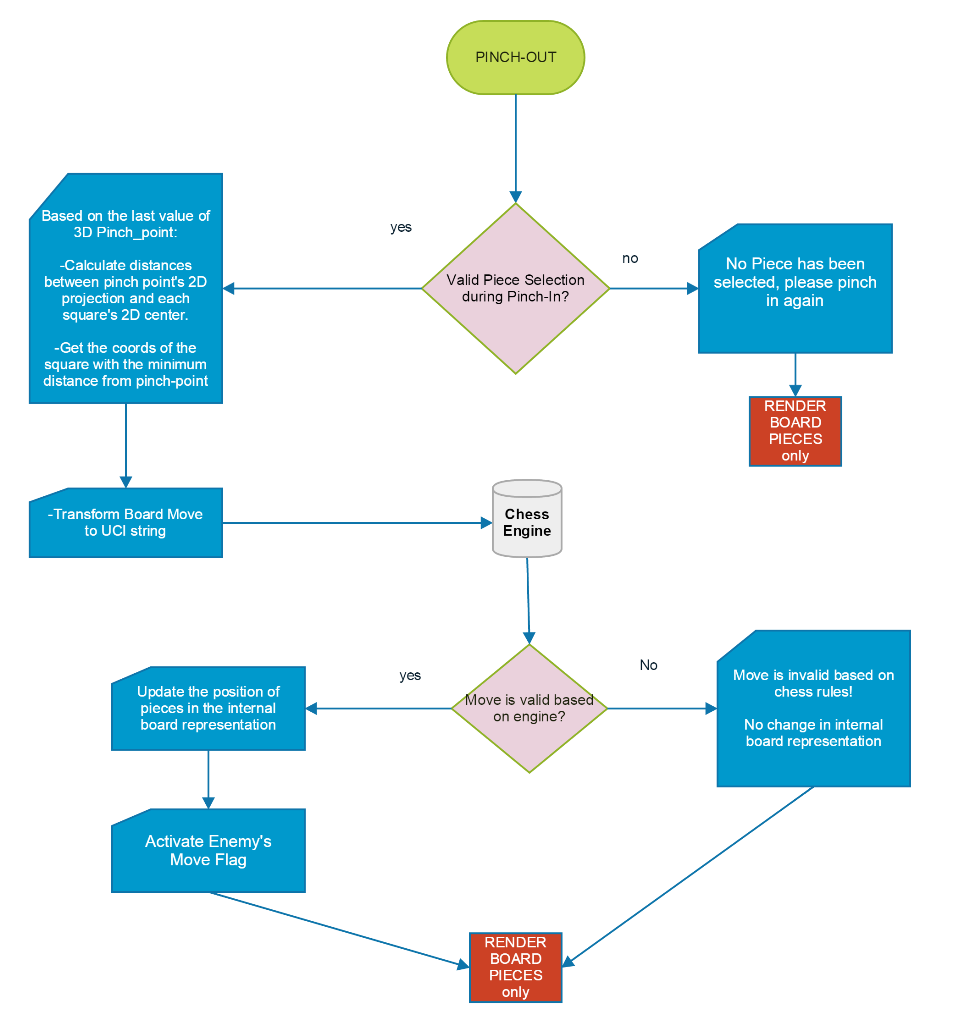
\includegraphics[width=0.85\textwidth]{Files/Figures/pinch_out.png}
    \caption[Διάγραμμα ροής κατάστασης Pinch-Out]{Διάγραμμα ροής κατάστασης Pinch-Out}
    \label{fig:pinch_out}
\end{figure}



Η τελευταία κατάσταση, για να ολοκληρωθεί ένα γύρος του παιχνιδιού, είναι η Enemy-Move, όπου χρειάζεται η εκτίμηση μιας κίνησης από τη μηχανή σκακιού για τα πιόνια του αντιπάλου. Η κίνηση, όπως αυτή παράγεται από τη μηχανή, εμφανίζεται σε μορφή συμβατή με το πρωτόκολλο UCI. Επομένως χρειάζεται ένας απλός μετασχηματισμός, από μία συμβολοσειρά σε μία σειρά αριθμών που θα δοθούν ως είσοδος στην εσωτερική δομή της διάταξης για να πραγματοποιηθεί μία κίνηση.
Έπειτα, ξεκινά to animation της κίνησης του πιονιού του αντιπάλου, που βασίζεται στην αρχή της παρεμβολής ανάμεσα στην αρχικό και το τελικό τετράγωνο της κίνησης. Τελικά, απεικονίζονται όλα τα πιόνια της ανανεωμένης διάταξης πιονιών.


\begin{figure}[H]
    \centering
    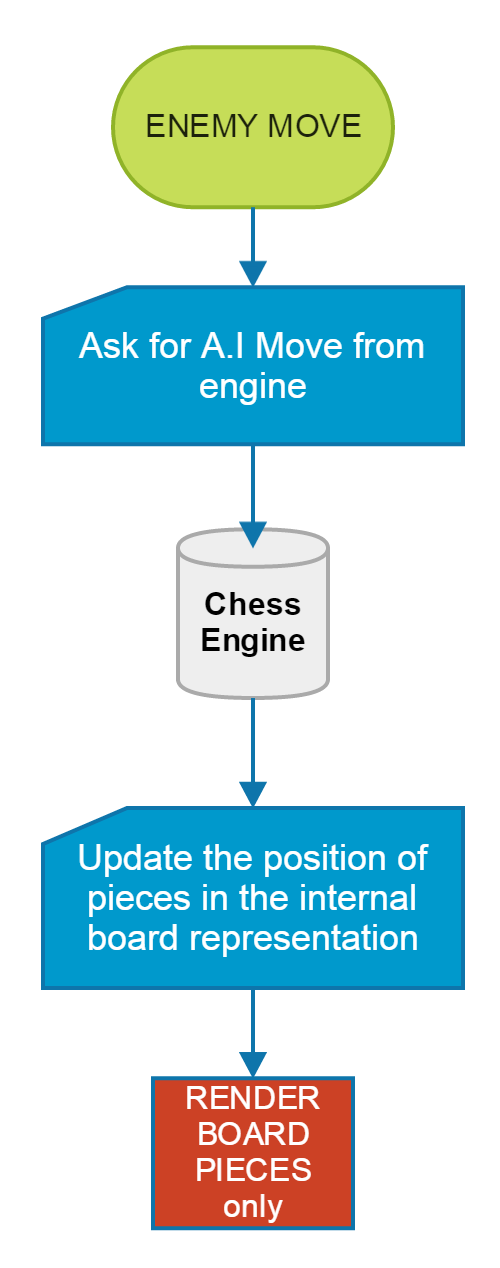
\includegraphics[scale=0.3]{Files/Figures/enemy_move.png}
    \caption[Διάγραμμα ροής κατάστασης Enemy-Move]{Διάγραμμα ροής κατάστασης Enemy-Move}
    \label{fig:enemy_move}
\end{figure}


\section{Αντιμετώπιση Απόκρυψης Αντικειμένων} \label{s:occlusion}
%OCCLUSION HANDLING



%-----
Για να μπορέσει ένας χρήστης να εκτελέσει επιτυχώς ορισμένες διεργασίες σε περιβάλλοντα επαυξημένης πραγματικότητας, χρειάζεται να παρέχεται από το σύστημα ένα συγκεκριμένο επίπεδο "εμβύθισης" του χρήστη. Πρέπει δηλαδή ο χρήστης να πιστέψει, όσο γίνεται, ότι τα εικονικά αντικείμενα είναι πραγματικά. 


Στις περισσότερες προσεγγίσεις, οι αποκρύψεις των εικονικών αντικειμένων δεν λαμβάνονται υπόψη και επομένως τα εικονικά αντικείμενα απεικονίζονται πάντα πάνω από το frame του βίντεο, συνεπώς πάνω από τα πραγματικά αντικείμενα της σκηνής. 
Ωστόσο, για να δημιουργηθούν καθηλωτικές και ρεαλιστικές εφαρμογές, η απόκρυψη ανάμεσα στα εικονικά και τα πραγματικά αντικείμενα πρέπει να πραγματοποιηθεί σωστά, ώστε οι χρήστες να μπορούν να κοιτάξουν σε μία σκηνή, όπου το εικονικό περιεχόμενο θα είναι εναρμονισμένο με το φυσικό περιβάλλον. Μία τέτοια προσέγγιση μας επιτρέπει να πετύχουμε υψηλό επίπεδο "εμβύθισης" αφού τα εικονικά αντικείμενα μπορούν να εναρμονιστούν με τα χέρια του χρήστη, ώστε να εμφανίζεται σωστά το ένα πάνω από το άλλο ή το αντίθετο. 

Κάτι τέτοιο συνήθως δε συμβαίνει στις περισσότερες εφαρμογές επαυξημένης πραγματικότητας. Στην OpenGL, όταν ένα αντικείμενο απεικονίζεται στην οθόνη, το βάθος ενός pixel που παράγεται (z coordinate) αποθηκεύεται σε ένα buffer που ονομάζεται z-buffer ή buffer βάθους (depth buffer). Αυτός ο buffer ορίζεται συνήθως ως ένα δισδιάστατος πίνακας (x-y) με ένα στοιχείο για κάθε εικονοστοιχείο της οθόνης. Αν κάποιο άλλο αντικείμενο της σκηνής πρέπει να απεικονιστεί στο ίδιο εικονοστοιχείο, η μέθοδος συγκρίνει τα 2 βάθη και αντικαθιστά το τρέχων εικονοστοιχείο, αν το αντικείμενο είναι πιο κοντά στο θεατή. Έπειτα, το επιλεγμένο βάθος αποθηκεύεται στο z-buffer, αντικαθιστώντας την προηγούμενη τιμή. Εν τέλει, ο z-buffer θα επιτρέψει στη μέθοδο να αναπαράγει σωστά την αντίληψη του βάθους, δηλαδή το γεγονός ότι ένα αντικείμενο που βρίσκεται πιο κοντά θα πρέπει να κρύβει ένα άλλο που βρίσκεται πιο μακριά.


Το κύριο πρόβλημα που εμφανίζεται και εμποδίζει την αντιμετώπιση του φαινομένου της απόκρυψης στα επαυξημένα περιβάλλοντα βρίσκεται στο γεγονός ότι, συνήθως, δεν υπάρχει πληροφορία για το βάθος της σκηνής. Για να ξεπεραστεί αυτό το πρόβλημα, πρέπει να αξιοποιηθεί το βάθος της πραγματικής σκηνής ως προς τη θέση του χρήστη. 

Στην παρούσα διπλωματική εργασία, χρησιμοποιήθηκε ο αισθητήρας βάθους της κάμερας Realsense 3D, για την υποστήριξη της διαδικασίας απόκτησης ενός χάρτη βάθους της σκηνής του περιβάλλοντος. O αισθητήρας αυτός μπορεί να μετρήσει την απόσταση κάθε αντικειμένου που βλέπει, δημιουργώντας ένα χάρτη βάθους. Με αυτό τον τρόπο το βάθος κάθε pixel του depth frame μπορεί να εκτιμηθεί. Η εικόνα βάθους είναι ουσιαστικά ένας πίνακας διαστάσεων 640 x 480  όπου η τιμή κάθε pixel αναπαριστά την απόσταση της κάμερας βάθους από το συγκεκριμένο σημείο στο 3D χώρο (σε χιλιοστά). 



Το τέχνασμα που χρησιμοποιείται είναι η αρχικοποίηση του Z-Buffer της OpenGL με τις τιμές βάθους που παίρνουμε από τον αισθητήρα πριν την απεικόνιση ενός 3D εικονικού αντικειμένου και αφού απεικονίσουμε το πολύγωνο που δείχνει την έγχρωμη εικόνα που καταγράφει το βίντεο. Με αυτό τον τρόπο, όταν τα εικονικά πιόνια απεικονίζονται στην οθόνη, θα αποκρύπτονται από τα χέρια του χρήστη ή από οποιοδήποτε άλλο αντικείμενο περάσει από πάνω τους. 

Η διαδικασία αυτή μοιάζει με την προσομοίωση της απεικόνισης ενός ολόκληρου περιβάλλοντος 3D και τη χρήση των τιμών του z-buffer. Eπομένως, προκειμένου να αντιμετωπίσουμε το πρόβλημα της απόκρυψης αντικειμένων (occlusion handling) έπρεπε να αντιστοιχήσουμε ολόκληρο το χάρτη βάθους στην έγχρωμη εικόνα που καταγράφεται, να μετατρέψουμε τις τιμές βάθους από χιλιοστά σε μέτρα και μετά να γράψουμε κάθε τιμή στο z-buffer της OpenGL.


Ωστόσο, πριν φτάσουμε στο σημείο να γράψουμε στο z-buffer, πρέπει να λάβουμε υποψη μας το είδος της προβολής που χρησιμοποιείται από την OpenGL στην εφαρμογή μας (ορθή ή προοπτική). 


Στη συγκεκριμένη περίπτωση, το είδος της προβολής με την οποία απεικονίζονται τα εικονικά αντικείμενα της σκηνής είναι η προοπτική προβολή και πρέπει να τροποποιήσουμε τα δεδομένα αντίστοιχα. Σε αυτό το είδος προβολής, η σχέση ανάμεσα στην τιμή Z και το βάθος είναι μη-γραμμική και συγκεκριμένα της μορφής:



\begin{equation}
\begin{aligned}
depth=\frac{A}{Z}+B \\ \vspace{0.5cm}
A=\frac{Z_{far}Z_{near}}{Z_{far}-Z_{near}}\\ \vspace{0.5cm}
B=\frac{Z_{far}}{Z_{far}-Z_{near}}
\end{aligned}
\end{equation}

Τέλος πρέπει να προσέξουμε το γεγονός ότι τα σημεία μπροστά από το σημείο παρατήρησης (viewpoint) στην OpenGL έχουν αρνητικές τιμές συντεταγμένων στον άξονα Z. Αφού εφαρμόσουμε το μετασχηματισμό που αναφέρθηκε με την προηγούμενη εξίσωση, μπορούμε να γράψουμε τις τιμές των δεδομένων στον z-buffer. Μόλις συμβεί αυτό, παρατηρούμε ότι τα πραγματικά και τα εικονικά αντικείμενα "δένουν" αρμονικά μαζί στη σκηνή με αρκετά μεγάλη ακρίβεια, όπως φαίνεται στην εικόνα~\ref{fig:occlusion}.



\begin{figure}[H]
    \centering
    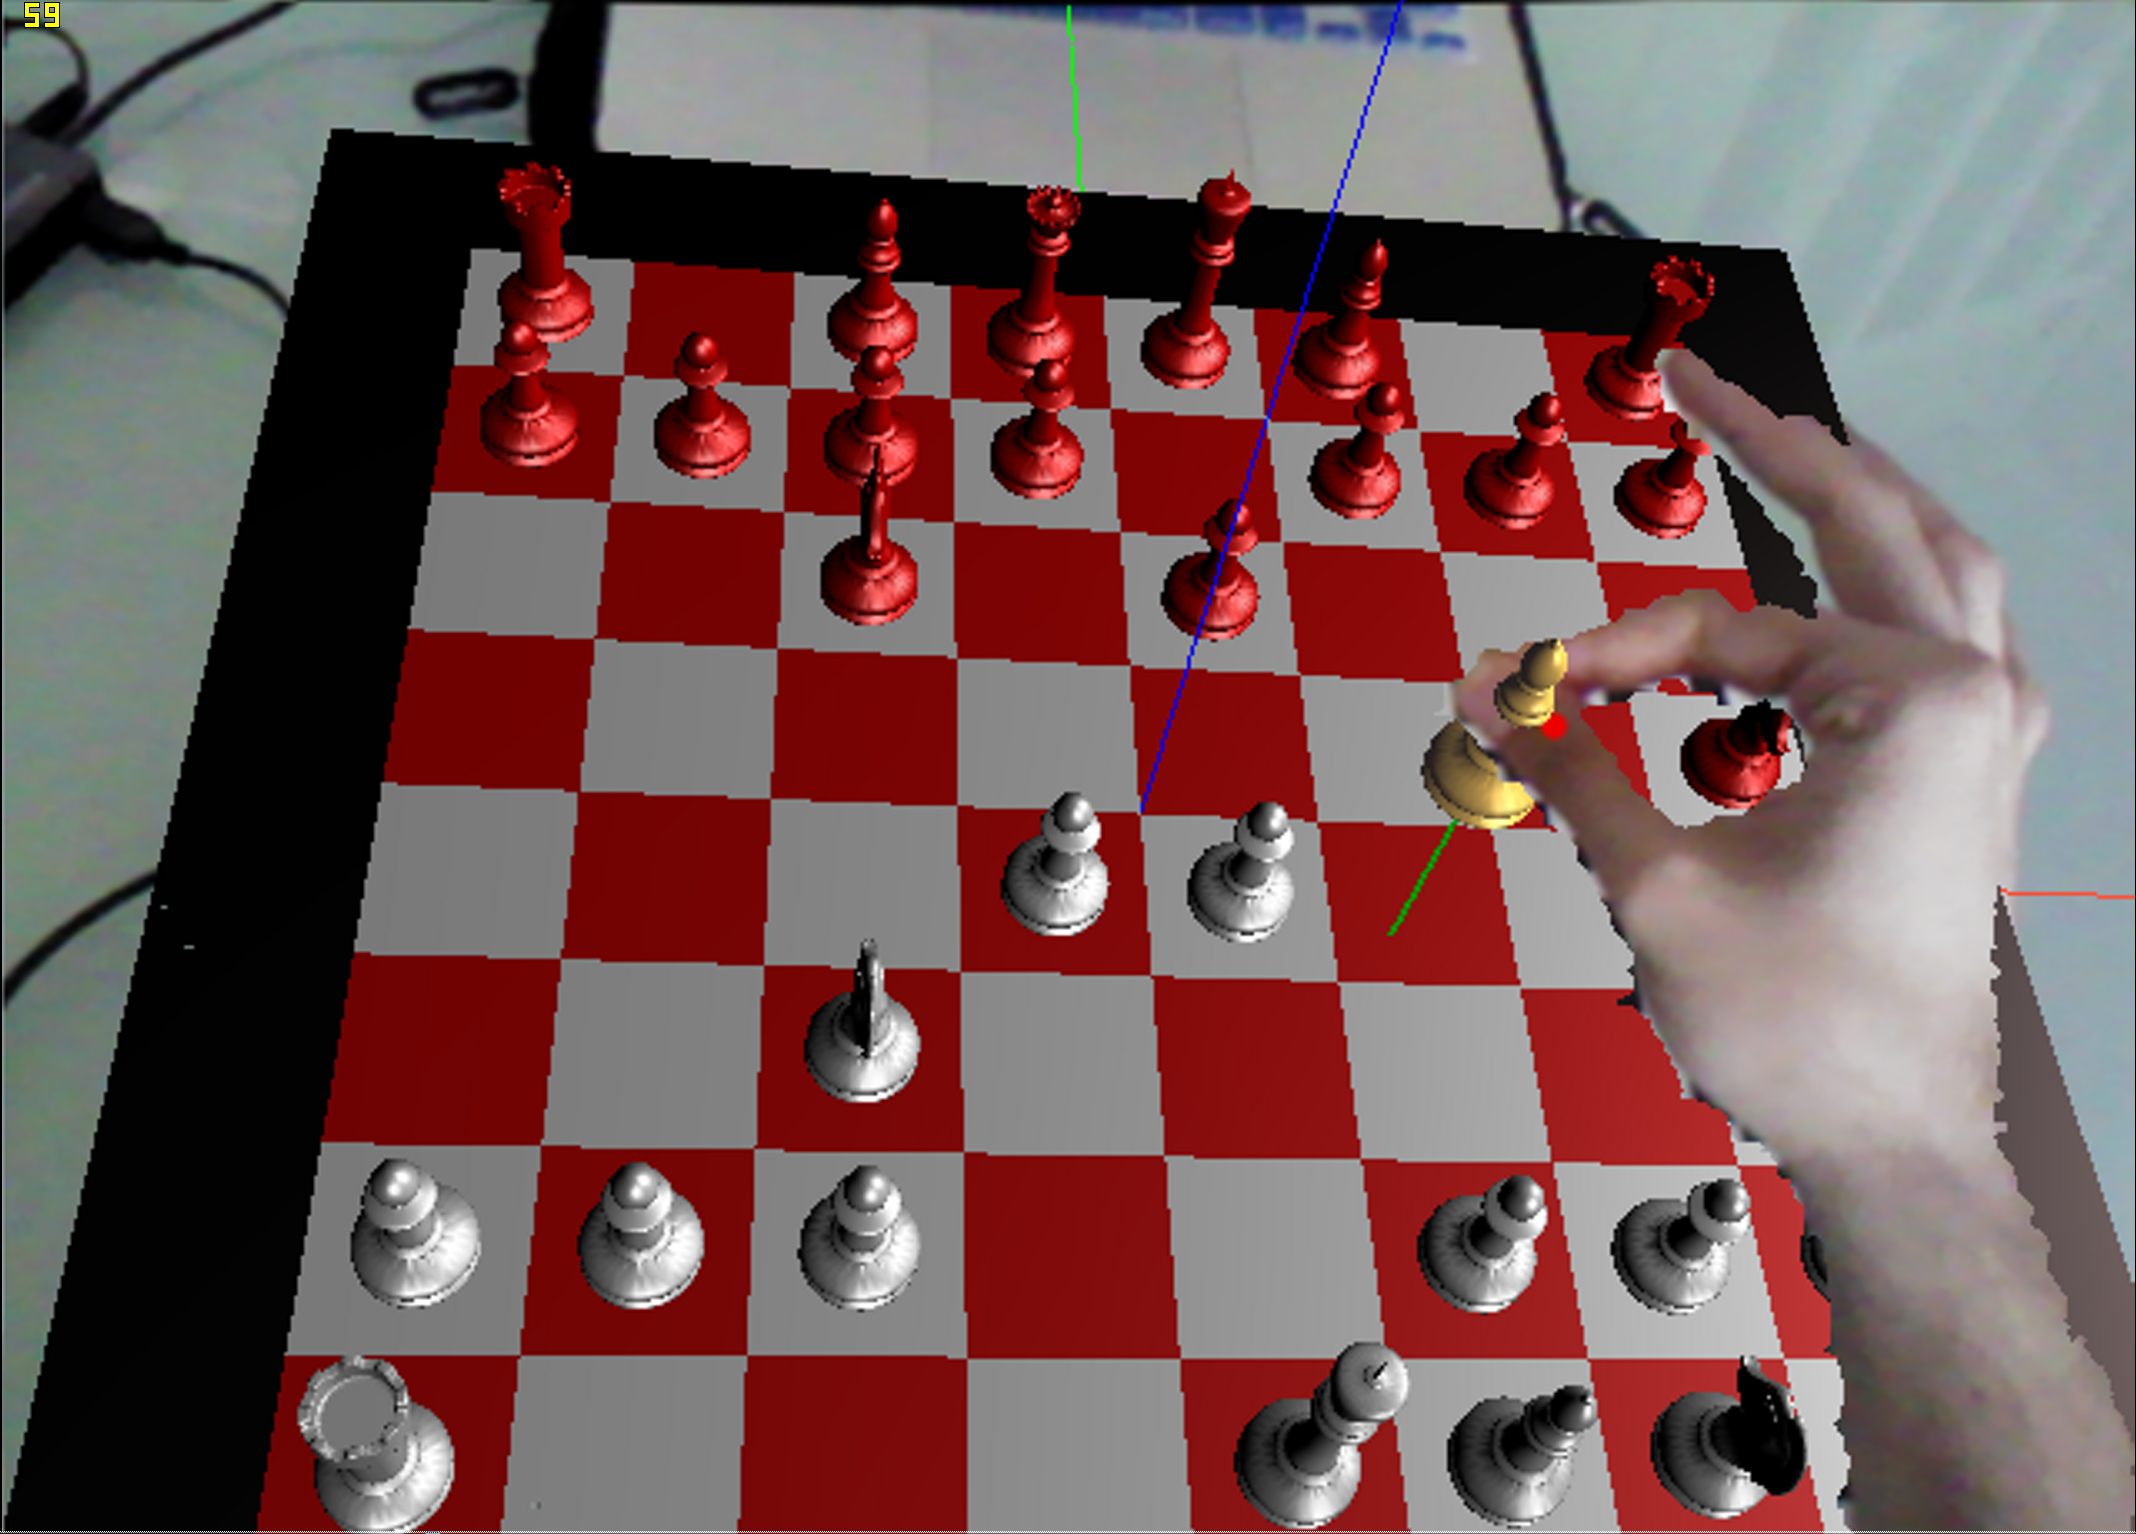
\includegraphics[width=0.55\textwidth]{Files/Figures/correct.png}
    \caption[Στιγμιότυπο της εφαρμογής που αναπτύχθηκε]{Στιγμιότυπο της εφαρμογής που αναπτύχθηκε}
    \label{fig:occlusion}
\end{figure}











 % 

%*******10********20********30********40********50********60********70********80

% For all chapters, use the newdefined chap{} instead of chapter{}
% This will make the text at the top-left of the page be the same as the chapter

\chap{Αξιολόγηση \& Συμπεράσματα}

Στην ενότητα αυτή, παρουσιάζονται και περιγράφονται τα πειραματικά αποτελέσματα που βρέθηκαν μέσω της αξιολόγησης του συστήματος, καθώς και οι περιορισμοί και τα συμπεράσματα που προκύπτουν από τη χρήση του. Η δοκιμή του συστήματος αναγνώρισης της χειρονομίας "τσιμπήματος" ενσωματώθηκε στη δοκιμή ολόκληρης της εφαρμογής σκακιού και επομένως η αξιολόγηση πραγματοποιήθηκε στο σύνολο του συστήματος.


%---



\section{Αξιολόγηση}



Η παρούσα διπλωματική εργασία δίνει έμφαση στην αξιολόγηση του συστήματος που αναπτύχθηκε, δηλαδή στο σκάκι επαυξημένης πραγματικότητας.
Στη συγκεκριμένη ενότητα παρουσιάζονται τα αποτελέσμα της αξιολόγησης μέσω της μεθόδου SUS, καθώς και τα αποτελέσματα από τα ερωτηματολόγια που συμπλήρωσαν οι χρήστες μετά τις δοκιμές που πραγματοποίησαν με την εφαρμογή σκακιού επαυξημένης πραγματικότητας. Επίσης έγιναν μετρήσεις των χρόνων για την ολοκλήρωση κάθε κίνησης χειρισμού των αντικειμένων και το ποσοστό των σωστών έναντι των λανθασμένων κινήσεων που μπόρεσε να κάνει κάθε χρήστης.


Συγκεκριμένα, συμμετείχαν 10 άτομα ηλικίας 20-25 ετών που γνώριζαν πώς παίζεται το επιτραπέζι παιχνίδι του σκακιού. Στην αρχή έγινε μια επεξήγηση που αφορούσε τον τρόπο λειτουργίας του συστήματος και τον τρόπο με τον οποίο πρέπει να πραγματοποιείται η χειρονομία "τσιμπήματος" για να μετακινηθεί ένα πιόνι στη σκακιέρα. Έπειτα, τους δόθηκε ένα διάστημα 1 λεπτών να εξοικειωθούν με το περιβάλλον επαυξημένης πραγματικότητας και να πραγματοποιήσουν μερικές δοκιμαστικές κινήσεις.

Οι οδηγίες που δόθηκαν στους χρήστες για την σωστή επιλογή και το χειρισμό των εικονικών αντικειμένων είχε ως εξής:

\begin{enumerate}
 
\item Τεντώστε το χέρι σας πάνω από το τραπέζι σε ύψος περίπου 15 εκατοστών.
\item Χρησιμοποιήστε το δεξί σας χέρι και πραγματοποιήστε τη χειρονομία "τσιμπήματος" κοντά σε ένα πιόνι για να το επιλέξετε. Η χειρονομία αυτή πρέπει να πραγματοποιείται με τέτοιο τρόπο, ώστε η οπή που σχηματίζεται από τον αντίχειρα και τον δείκτη να είναι πάντα ορατή από την κάμερα και τα υπόλοιπα δάκτυλα να είναι τεντωμένα και να μην πραγματοποιούν την ίδια κίνηση με τον δείκτη. Τα εικονικά πιόνι χρωματίζονται χρυσά αν επιλεγούν.
\item Μετακινήστε το πιόνι που επιλέξατε πάνω από ένα άλλο τετράγωνο της εικονικής σκακιέρας, με τον ίδιο τρόπο με τον οποίο θα παίζατε σκάκι με πραγματικά πιόνια και πραγματική σκακιέρα. 
\item Σταματήστε την χειρονομία κατά την οποία ο δείκτης και ο αντίχειρας αγγίζουν ο ένας τον άλλον, ώστε να απελευθερωθεί το αντικείμενο. Το εικονικό πιόνι θα τοποθετηθεί στο τετράγωνο που βρίσκεται πιο κοντά από το σημείο στο οποίο αφήνεται το πιόνι.
\end{enumerate}

\subsection{Αξιολόγηση SUS}


Η αξιολόγηση του συστήματος αναγνώρισης χειρονομιών που αναπτύχθηκε, περιορίστηκε σε ερωτήσεις προς τους χρήστες μέσω ερωτηματολογιών χρηστικότητας σε σχέση με τις χειρονομίες. Οι χρήστες δοκίμασαν για πρώτη φορά την εφαρμογή κατά το στάδιο της αξιόλογησης, ωστόσο είχαν τη δυνατότητα να μάθουν πώς λειτουργεί και να εξοικειωθούν με το περιβάλλον επαυξημένης πραγματικότητας σε μία περίοδο διάρκειας 10 λεπτών. Ο χρόνος αυτός θεωρήθηκε αρκετός για να μάθουν να χρησιμοποιούν το σύστημα αναγνώρισης χειρονομιών σωστά και να μπορούν να μετακινούν εικονικά πιόνια στην εικονική σκακιέρα. 


Προκειμένου να μπορέσουμε να αξιολογήσουμε τη εφαρμογή σκακιού επαυξημένης πραγματικότητας που αναπτύχθηκε, χρησιμοποιήθηκε η μέθοδος "Κλίμακας Χρησιμότητας Συστήματος" (System Usability Scale - SUS). Η μέθοδος αυτή περιλαμβάνει ένα ερωτηματολόγιο με 10 ερωτήσεις προς τους χρήστες, με στόχο τη μέτρηση της ευκολίας χρήσης ενός συστήματος λογισμικού, hardware, κινητών τηλεφώνων ή ιστοσελίδων και παρουσιάστηκε από τον John Brooke \cite{Brooke1996}. Πρόκειται για μία τεχνολογία η οποία έχει δοκιμαστεί σε πολλές εφαρμογές και θεωρείται πλέον standard της βιομηχανίας, με αναφορές σε περισσότερες από 600 επιστημονικές δημοσιεύσεις. 


Το ερωτηματολόγιο SUS αποτελείται, όπως είπαμε, από 10 ερωτήσεις (στην αγγλική γλώσσα). Ο χρήστης καλείται να απαντήσει σε κάθε ερώτηση, καθεμια από τις οποίες έχει 5 πιθανές απαντήσεις όπως φαίνεται στην εικόνα~\ref{fig:answers}


\begin{figure}[H]
    \centering
    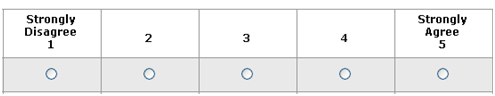
\includegraphics[width=0.8\textwidth]{Files/Figures/sus-responses.png}
    \caption[Πιθανές απαντήσεις ερωτηματολογίου SUS]{Πιθανές απαντήσεις ερωτηματολογίου SUS}
    \label{fig:answers}
\end{figure}




Η βαθμολογία SUS προκύπτει ως εξής:
\begin{itemize}
\item Για τις ερωτήσεις με περιττό αριθμό: Αφαιρείται μία μονάδα από την τιμή της απάντησης (1-5).
\item Για τις ερωτήσεις με άρτιο αριθμό: Αφαιρείται η τιμή της απάντησης από τον αριθμό 5.
\item  Προσθέτοντας τις τιμές των απαντήσεων για κάθε χρήστη και πολλαπλασιάζοντας το σύνολο με 2.5, παίρνουμε ένα εύρος τιμών από το 0 ως το 100.
\end{itemize}




Η αξιολόγηση ενός συστήματος μέσω της μεθόδου SUS θεωρείται έγκυρη και αξιόπιστη. Στόχος αυτού του συστήματος αξιολόγησης είναι να παρέχει ένα εύκολο τεστ προς συμπλήρωση στους χρήστες που δοκιμάζουν το σύστημα και να επιτρέψει συγκρίσεις μεταξύ προϊόντων και εφαρμογών, με απώτερο σκοπό την αντικειμένική αξιολόγηση της χρηστικότητας του συστήματος. 


Το αποτέλεσμα της αξιολόγησης SUS για το σύστημά μας ήταν 73.25 με τυπική απόκλιση 10.7 και μέσο 75, το οποίο με βάση το \cite{bangor2008empirical} σημαίνει ότι έχουμε ένα αποδεκτό αποτέλεσμα (χρειάζεται να έχουμε ποσοστό μεγαλύτερο από 70\%).


Τα αποτελέσματα φαίνονται στις παρακάτω εικόνες. Στην πρώτη απεικονίζονται οι απαντήσεις που έδωσε κάθε χρήστης, ενώ στη δεύτερη το συνολικό αποτέλεσμα.

\begin{center}
\begin{tabular}{ |c||c|c|c|c|c|c|c|c|c|c||c|  }
\hline
 \multicolumn{12}{|c|}{System Usability Scale Results} \\
\hline
User   & Q1 & Q2 & Q3 & Q4 & Q5 & Q6 & Q7 & Q8 & Q9 & Q10 & SUS Score\\
 \hline
 User1   & 4    & 2 &   4 &   1 &   4 &   2 &   5 &   4 &   4 &   2 &   75.0\\
 User2   & 3    & 2 &   3 &   2 &   3 &   3 &   3 &   3 &   2 &   2 &   55.0\\
 User3   & 3    & 2 &   4 &   1 &   4 &   3 &   5 &   1 &   4 &   1 &   80.0\\
 User4   & 5    & 1 &   4 &   1 &   4 &   1 &   5 &   1 &   4 &   1 &   92.5\\
 User5   & 3    & 1 &   4 &   1 &   4 &   2 &   4 &   2 &   4 &   1 &   80.0\\
 User6   & 4    & 2 &   4 &   3 &   4 &   2 &   3 &   3 &   4 &   2 &   67.5\\
 User7   & 2    & 1 &   3 &   1 &   5 &   2 &   4 &   2 &   3 &   1 &   75.0\\
 User8   & 2    & 2 &   2 &   1 &   4 &   2 &   4 &   3 &   2 &   2 &   60.0\\
 User9   & 2    & 2 &   3 &   1 &   4 &   1 &   4 &   2 &   3 &   2 &   70.0\\
 User10   & 3    & 1 &   3 &   1 &   5 &   2 &   4 &   2 &   3 &   1 &   77.5\\
\hline
\end{tabular}
\end{center}


\begin{figure}[H]
    \centering
    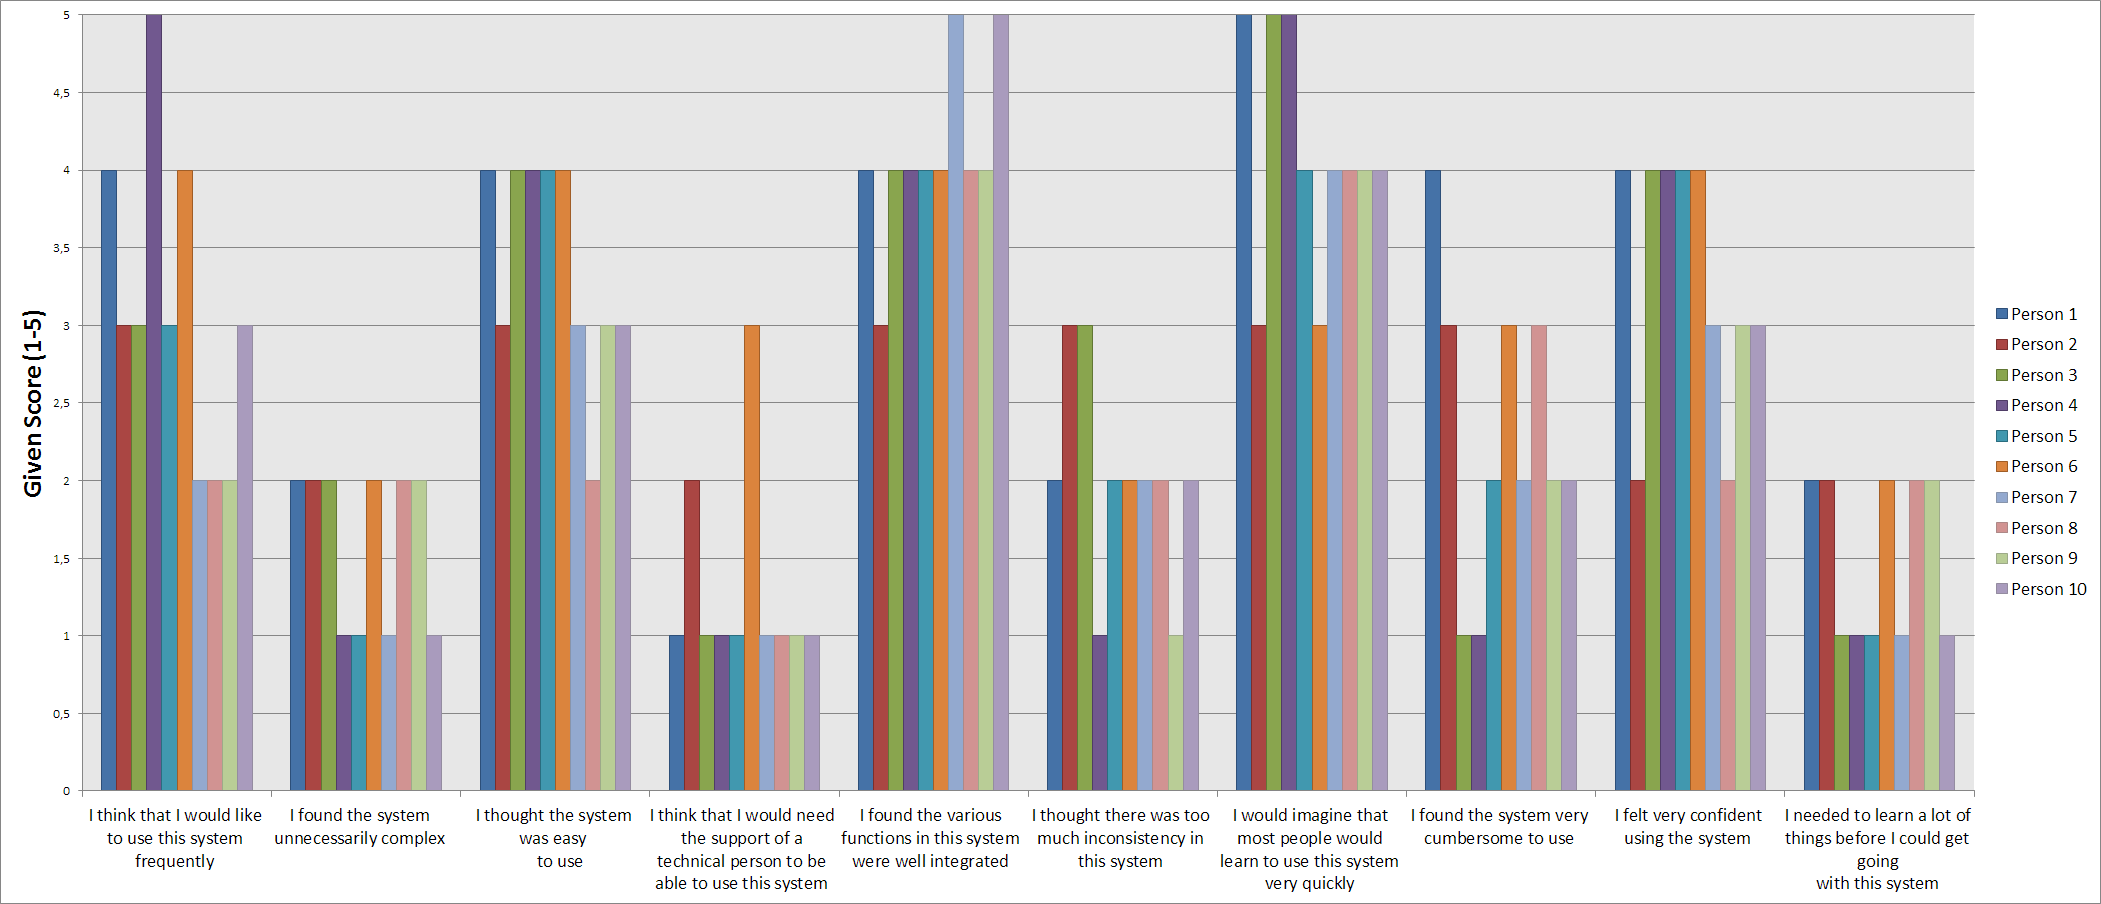
\includegraphics[width=0.99\textwidth]{Files/Figures/sus_per_person.png}
    \caption[Απαντήσεις των χρηστών στο ερωτηματολόγιο SUS]{Απαντήσεις των χρηστών στο ερωτηματολόγιο SUS}
    \label{fig:markerboard}
\end{figure}





Η αξιολόγηση έδειξε ότι το σύστημα είναι χρηστικό ως μηχανισμός εισόδου σε μία διεπαφή επαυξημένης πραγματικότητας στον τρισδιάστατο χώρο, παρά το γεγονός ότι το σύστημα δεν έχει βελτιστοποιηθεί ακόμα ως προς τη λειτουργικότητά του, αφού οι χρήστες μπόρεσαν επιτυχημένα να μετακινήσουν τα πιόνια στη σκακιέρα και να παίξουν ενάντια στον υπολογιστή. 

\begin{figure}[H]
    \centering
    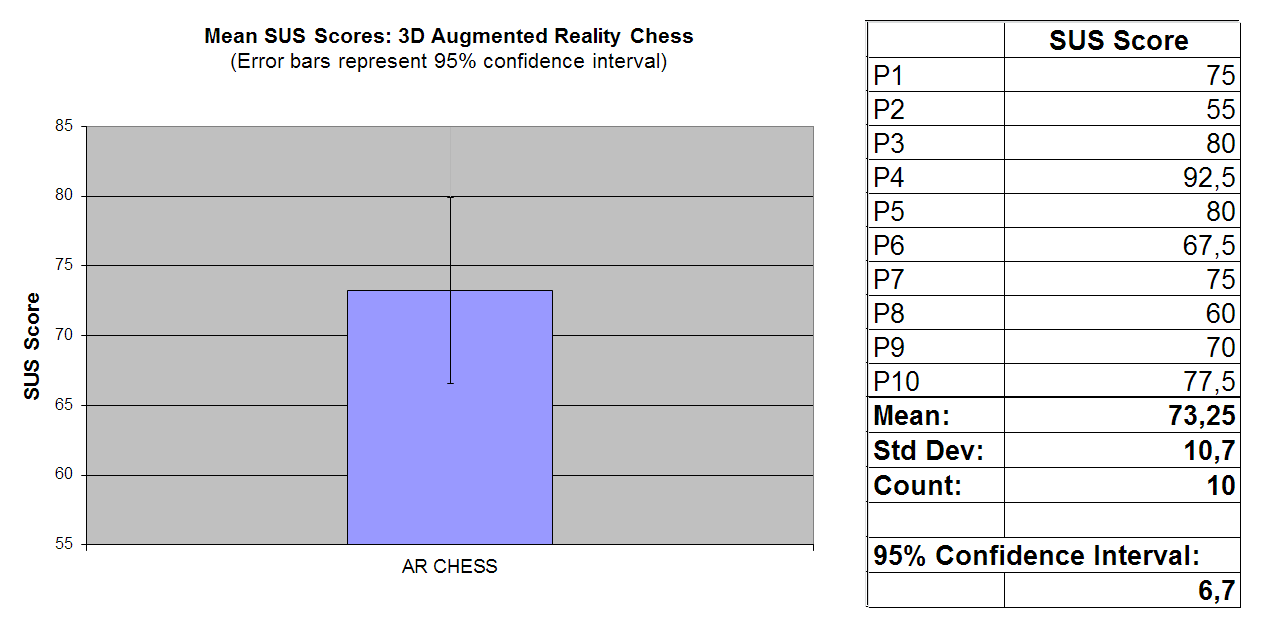
\includegraphics[width=0.98\textwidth]{Files/Figures/sus.png}
    \caption[Μέση τιμή και λεπτομέρειες σχετικά με το αποτέλεσμα της αξιολόγησης SUS]{Μέση τιμή και λεπτομέρειες σχετικά με το αποτέλεσμα της αξιολόγησης SUS}
    \label{fig:sus_res}
\end{figure}


\subsection{Χρόνος και Επιτυχία Ολοκλήρωσης Κινήσεων}


Στη δεύτερη φάση της αξιολόγησης, μετρήσαμε τον αριθμό των χειρονομιών "τσιμπήματος" που χρειάστηκε να κάνει κάθε χρήστης μέχρι να γίνει η σωστή επιλογή του εικονικού αντικειμένου. Πέρα από αυτό, έγινε μέτρηση του χρόνου που χρειάστηκε κάθε χρήστης για να μετακινήσει ένα εικονικό πιόνι από τη στιγμή που το επέλεξε. Τέλος, θέλαμε να βρούμε κατά πόσο το σύστημα μας είναι αξιόπιστο, δηλαδή κατά πόσο το σύστημά μας καταλαβαίνει, με βάση την κίνηση του χρήστη, σε ποιο τετράγωνο θέλησε ο χρήστης να αφήσει το πιόνι, όπως αναφέρθηκε και σε προηγούμενη ενότητα. Τα αποτελέσματα φαίνονται στον παρακάτω πίνακα.


\begin{table}[h]
\centering
\caption{My caption}
\label{my-label}
\begin{adjustbox}{max width=\textwidth}
\begin{tabular}{|r|r|r|r|r|r|r|}
\hline
\multicolumn{1}{|c|}{{\bf \begin{tabular}[c]{@{}c@{}}Participant\\   \#\end{tabular}}} & \multicolumn{1}{c|}{{\bf \begin{tabular}[c]{@{}c@{}}Time per \\ Correct Move\\   (sec)\end{tabular}}} & \multicolumn{1}{c|}{{\bf \begin{tabular}[c]{@{}c@{}}Tasks Completed\\   (out of 30)\end{tabular}}} & \multicolumn{1}{c|}{{\bf Time \%}} & \multicolumn{1}{c|}{{\bf Tasks \%}} & \multicolumn{1}{c|}{{\bf SUS Rating \%}} & \multicolumn{1}{c|}{{\bf Average}} \\ \hline
1                                                                                      & 2,99                                                                                                  & 25                                                                                                 & 83\%                               & 83\%                                & 75\%                                     & 81\%                               \\ \hline
2                                                                                      & 4,23                                                                                                  & 25                                                                                                 & 59\%                               & 83\%                                & 55\%                                     & 66\%                               \\ \hline
3                                                                                      & 3,05                                                                                                  & 16                                                                                                 & 82\%                               & 53\%                                & 80\%                                     & 72\%                               \\ \hline
4                                                                                      & 4,94                                                                                                  & 25                                                                                                 & 50\%                               & 83\%                                & 92,5\%                                   & 75\%                               \\ \hline
5                                                                                      & 3,49                                                                                                  & 25                                                                                                 & 71\%                               & 83\%                                & 80\%                                     & 78\%                               \\ \hline
6                                                                                      & 5,64                                                                                                  & 22                                                                                                 & 44\%                               & 73\%                                & 67,5\%                                   & 62\%                               \\ \hline
7                                                                                      & 2,49                                                                                                  & 18                                                                                                 & 100\%                              & 60\%                                & 75\%                                     & 78\%                               \\ \hline
8                                                                                      & 4,66                                                                                                  & 28                                                                                                 & 53\%                               & 93\%                                & 60\%                                     & 69\%                               \\ \hline
9                                                                                      & 2,74                                                                                                  & 28                                                                                                 & 91\%                               & 93\%                                & 70\%                                     & 85\%                               \\ \hline
10                                                                                     & 3,00                                                                                                  & 26                                                                                                 & 83\%                               & 87\%                                & 77,5\%                                   & 82\%                               \\ \hline
{\bf Averages}                                                                         & {\bf 3,723}                                                                                           & {\bf 23,8}                                                                                         & {\bf 72\%}                         & {\bf 79\%}                          & {\bf 73\%}                               & {\bf 75\%}                         \\ \hline
\end{tabular}
\end{adjustbox}
\end{table}





\begin{figure}[H]
    \centering
    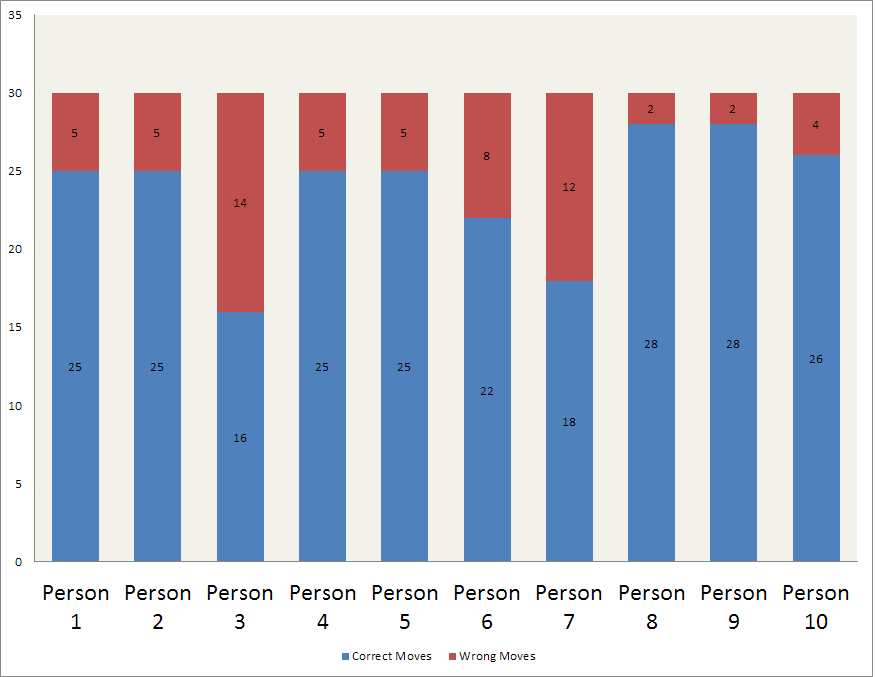
\includegraphics[width=0.95\textwidth]{Files/Figures/correctmoves.png}
    \caption[Σχέση ανάμεσα σε σωστές και λανθασμένες κινήσεις χρηστών]{Σχέση ανάμεσα σε σωστές και λανθασμένες κινήσεις χρηστών}
    \label{fig:correctmoves}
\end{figure}



Παρά το γεγονός ότι οι διαδοχικές κινήσεις ενός παίκτη στο σκάκι, συνήθως δεν έχουν κάποια συνοχή, τα αποτελέσματα κρίνονται ιδιαίτερα ικανοποιητικά. Ο μέσος χρόνος εκτέλεσης μιας κίνησης βρέθηκε κοντά στα 3.7 δευτερόλεπτα, επομένως μπορούμε να πούμε ότι η αλληλεπίδραση του χρήστη με το σύστημα φαίνεται αρκετά φυσική. 


Ωστόσο, παρατηρήθηκε ότι οι λανθασμένες κινήσεις ξεπέρασαν τις προσδοκίες μας, ειδικά όταν οι χρήστες προσπαθούσαν να πραγματοποιήσουν μεγάλες κινήσεις σε αποστάσεις μεγαλύτερες των 3 τετραγώνων της σκακιέρας. Για το συγκεκριμένο λόγο, προτάθηκε μία λύση, η οποία παρουσιάζεται στην ενότητα~\ref{sec:conclusion}. Η προσθήκη ενός buffer που θα περιμένει μέχρι να βρεθούν ορισμένα διαδοχικά frames χωρίς να ανιχνεύεται χειρονομία "τσιμπήματος" για να προχωρήσει σε κατάσταση Pinch-Out κρίθηκε επιτακτική. Οι λανθασμένες κινήσεις μειώθηκαν αισθητά όπως φαίνεται στην εικόνα~\ref{fig:correctmoves2}

\begin{figure}[H]
    \centering
    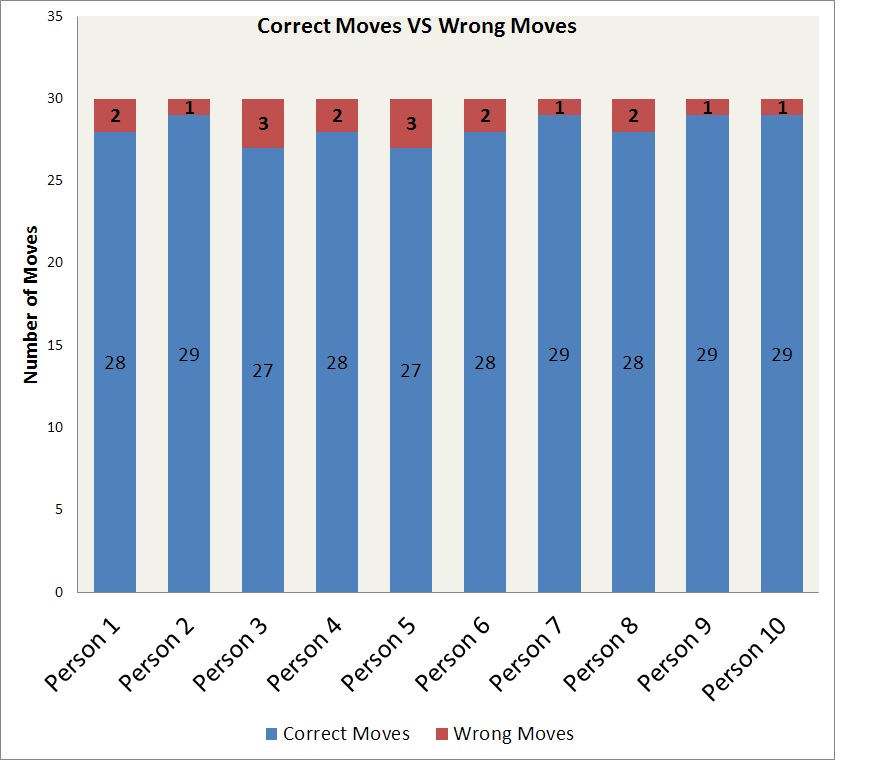
\includegraphics[width=0.95\textwidth]{Files/Figures/correctmoves2.png}
    \caption[Σχέση ανάμεσα σε σωστές και λανθασμένες κινήσεις χρηστών μετά την προσθήκη buffer]{Σχέση ανάμεσα σε σωστές και λανθασμένες κινήσεις χρηστών μετά την προσθήκη buffer}
    \label{fig:correctmoves2}
\end{figure}




\subsection{Ερωτηματολόγια}

Για να μπορέσουμε να αξιολογήσουμε με περισσότερη ακρίβεια το σύστημα που αναπτύχθηκε και την εμπειρία των χρηστών, μοιράστηκε στους χρήστες που δοκίμασαν την εφαρμογή ένα ανοιχτό ερωτηματολόγιο, το οποίο συμπλήρωσαν αμέσως μετά το τέλος της δοκιμής. Ζητήθηκε από τους χρήστες να δηλώσουν παρόμοιες εμπειρίες με εφαρμογές επαυξημένης πραγματικότητας και συστήματα αλληλεπίδρασης μέσω χειρονομιών. Το ερωτηματολόγιο που μοιράστηκε, αφορούσε την εμπειρία των χρηστών ως προς την απόδοση της αναγνώρισης χειρονομιών του συστήματος και το επίπεδο "εμβύθισής" τους στο περιβάλλον επαυξημένης πραγματικότητας. 


Οι περισσότεροι χρήστες από αυτούς που δοκίμασαν την εφαρμογή δεν είχαν παρόμοια εμπειρία ούτε από χρήση συστημάτων επαυξημένης πραγματικότητας, ούτε από συστήματα αναγνώρισης χειρονομιών.
Όσον αφορά την απόκριση της συστήματος ως προς την αναγνώριση των χειρονομιών, οι περισσότεροι χρήστες θεώρησαν ότι πραγματοποιείται αρκετά άμεσα, ενώ παράλληλα θεώρησαν ότι η απεικόνιση των αντικειμένων με βάση το χάρτη βάθους της σκηνής εξυπηρετεί το σκοπό της εφαρμογής που είναι η "εμβύθιση" του χρήστη και η ευκολία επιλογής των πιονιών, προσφέροντας μία ρεαλιστική εμπειρία.

Συγκεκριμένα ως προς το χειρισμό των εικονικών αντικειμένων, οι χρήστες απάντησαν θετικά ως προς την ευκολία επιλογής ενός εικονικού πιονιού στο περιβάλλον της εφαρμογής, αλλά και ως προς την ευκολία μετακίνησής του στη σκακιέρα. Η πειραματική εγκατάσταση που χρησιμοποιήθηκε με το καπέλο και το markerboard μπροστά από το χρήστη φαίνεται ότι δεν δυσκόλεψε το χρήστη, αφού δεν περιλαμβάνονταν περιττά καλώδια ή περισσότερα markers, παρά μόνο τα χέρια τους για τη μετακίνηση των εικονικών αντικειμένων.


Τα ερωτηματολόγια έδειξαν ότι η χρήση της εφαρμογής δεν κούρασε τους χρήστες, ούτε το γεγονός ότι έπρεπε να πραγματοποιούν τη χειρονομία "τσιμπήματος" τοποθετώντας το χέρι τους με τέτοιο τρόπο ώστε η οπή που σχηματίζεται ανάμεσα σε δείκτη και αντίχειρα να βρίσκεται κάθεται προς τον αισθητήρα. Ουσιαστικά αρκούσε η ανάδραση που έπαιρναν από το σύστημα που δεν τους επέτρεπε να επιλέξουν ένα πιόνι, αν δεν πραγματοποιούσαν σωστά τη χειρονομία "τσιμπήματος". 

\begin{figure}[H]
    \centering
    \includegraphics[width=0.95\textwidth]{Files/Figures/questionnaire.png}
     \caption[Αποτελέσματα ανοιχτού ερωτηματολογίου]{Αποτελέσματα ανοιχτού ερωτηματολογίου}
    \label{fig:open}
\end{figure}




Οι χρήστες που δοκίμασαν να επιλέξουν σιγά σιγά τα πιόνια και μετά να δοκιμάσουν να τα μετακινήσουν, δεν είχαν κάποιο πρόβλημα και βελτιώθηκαν στη χρήση του συστήματος με το χρόνο, ενώ όσοι προσπάθησαν βιαστικά να τα επιλέξουν κουράστηκαν κατά τη διάρκεια του παιχνιδιού. Η πλειονότητα, πάντως, των ατόμων που δοκίμασαν την εφαρμογή συμφώνησε πως είναι απαραίτητη η εξάσκηση για τη χρήση του συστήματος σε ένα αρχικό στάδιο. Από εκεί και πέρα, ωστόσο, η διαδικασία απλοποιείται. Εξάλλου, κάθε νέα συσκευή ή τρόπος αλληλεπίδρασης με ένα σύστημα απαιτεί ένα χρονικό διάστημα για τη μάθηση της χρήσης του.


Την υψηλότερη βαθμολογία, στο ερωτηματολόγιο που δόθηκε στους χρήστες, συγκέντρωσε η ερώτηση σχετικά με το αν η εφαρμογή σκακιού που αναπτύχθηκε τους φάνηκε διασκεδαστική. Η υψηλή αυτή βαθμολογία δείχνει ότι η εφαρμογή που παρουσιάζεται στη συγκεκριμένη διπλωματική εργασία πετυχαίνει το στόχο της σχετικά με τη φυσική αλληλεπίδραση με το χρήστη και τη μεταφορά ενός κλασικού επιτραπέζιου παιχνιδιού σε περιβάλλον επαυξημένης πραγματικότητας.


Ίσως το κυριότερο πρόβλημα της εφαρμογής, λόγω της πειραματικής εγκατάστασης που χρησιμοποιήθηκε, βρίσκεται στην αίσθηση του βάθους στην επαυξημένη σκηνή, ως προς το σημείο παρατήρησης του χρήστη. Αυτό σημαίνει ότι, ενώ ο χρήστης είναι σίγουρος ότι το εικονικό αντικείμενο κινείται μέσω του χεριού του προς τα πίσω, στην πραγματικότητα κινείται προς τα πάνω. Όπως είπε ακριβώς ένας από τους χρήστες :"Όταν κατανοήσω που ακριβώς βρίσκεται το πιόνι στο χώρο κοιτώντας το markerboard, μπορώ να καταλάβω προς τα πού πρέπει να κινήσω το χέρι μου, το οποίο κρατάει το πιόνι στον εικονικό κόσμο.". Αυτή η σκέψη ήταν κοινή για αρκετούς από τους συμμετέχοντες και θεώρησαν ότι η χρήση ενός συστήματος Video See-Through HMD θα ήταν ιδανική για το σύστημα, αφού θα κοίταζαν προς το markerboard και θα έβλεπαν τα εικονικά πιόνια μέσω του HMD, επομένως θα μπορούσαν να έχουν καλύτερη αίσθηση του βάθους, σε σχέση με τη χρήση μιας οθόνης για την επαύξηση της σκηνής.



Τέλος, κάποιοι από τους χρήστες που δοκίμασαν την εφαρμογή και πρότειναν βελτιώσεις, θεώρησαν ότι μπορεί να βελτιωθεί το επίπεδο της απόκρυψης των αντικειμένων (occlusion) αν εφαρμοστεί κάποιο φίλτρο εξομάλυνσης στο χάρτη βάθους του αισθητήρα.







\section{Συμπεράσματα και Παρατηρήσεις} \label{sec:conclusion}


Κατά τη διάρκεια των δοκιμών προσομοίωσης του σκακιού της επαυξημένης πραγματικότητας που αναπτύχθηκε, παρουσιάστηκαν ορισμένοι περιορισμοί και μειονεκτήματα του συστήματος αλληλεπίδρασης, τα οποία οδήγησαν στον επανασχεδιασμό ορισμένων πτυχών της εφαρμογής. 


Αρχικά, αν κατά τη διαδικασία εξαγωγής blobs για την ανίχνευση του χεριού του χρήστη, αυτός αποφασίσει να επιλέξει ένα αντικείμενο και να το μετακινήσει, το χέρι του μπορεί να βρίσκεται πολύ κοντά στο τραπέζι. Αυτό έχει σαν αποτέλεσμα την αποτυχία αναγνώρισης της χειρονομίας "τσιμπήματος", αφού το πρόγραμμα θεωρεί το χέρι και τα δάκτυλα του χρήστη μαζί με το τραπέζι ή την επιφάνεια όπου βρίσκεται το markerboard ως ένα blob, συνολικά. Το ίδιο συμβαίνει αν χέρι του χρήστη είναι ορατό από τον αισθητήρα αλλά το μπράτσο του είναι κοντά στο τραπέζι με αποτέλεσμα μπράτσο, χέρι και τραπέζι να θεωρούνται ως ένα blob. Τότε το σύστημα, το οποίο προσπαθεί να βρει το κοντινότερο blob, μπορεί να μπερδευτεί και να μην μπορέσει να ανιχνεύσει κάποια Το πρόβλημα αυτό εμφανίζεται και σε άλλους αισθητήρες που χρησιμοποιούν παρόμοιες προσεγγίσεις αναγνώρισης χειρονομιών, όπως το Leap Motion. 

Ωστόσο, θεωρήθηκε ότι θα ήταν υπερβολικό να αλλάξουμε εντελώς τον τρόπο με τον οποίο το RealSense SDK εξάγει τα blobs. Σκεφτήκαμε ότι μπορούμε να αντιμετωπίσουμε το πρόβλημα με τον οπτικό σχεδιασμό μιας εικονικής σκακιέρας που έχει συνήθως κυβικό σχήμα, δηλαδή έχει ένα ορισμένο ύψος πάνω από την επιφάνεια του τραπεζιού. Συνεπώς, στην εφαρμογή του σκακιού επαυξημένης πραγματικότητας που παρουσιάζεται, απεικονίζεται μία σκακιέρα κάτω από τα εικονικά πιόνια, η οποία αποτελείται από μία διάταξη πολλαπλών κύβων με ύψος περίπου 3,5cm, αφού αυτό είναι το όριο ύψους πάνω από το οποίο μπορεί ο αισθητήρας να ανιχνεύσει σωστά το χέρι του χρήστη. 


Ακόμα ένα πρόβλημα που παρουσιάστηκε κατά τη διάρκεια των δοκιμών, αφορά το γεγονός ότι η λανθασμένη ανίχνευση του σημείου στο οποίο συνέβη η χειρονομία "τσιμπήματος" μπορεί να οδηγήσει στην ακούσια κίνηση ενός εικονικού πιονιού σε διαφορετική θέση από αυτή που επιδιώκει ο χρήστης. Τα αποτελέσματα έδειξαν ότι οι χρήστες συχνά εξέφραζαν παράπονα για το συγκεκριμένο πρόβλημα Για παράδειγμα, ο χρήστης μπορεί να ήθελε να μετακινήσει ένα απλό πιόνι - στρατιώτη 2 τετράγωνα μακριά από την αρχική του θέση. Ωστόσο, κατά τη διάρκεια αυτής της μετατόπισης, μπορεί σε κάποιο frame να μην ανιχνευόταν η χειρονομία "τσιμπήματος" και το σύστημα θεωρούσε ότι ο χρήστης ήθελε να απελευθερώσει το πιόνι νωρίτερα. Έτσι το σύστημα αποκρινόταν, αφήνοντας το πιόνι στο προηγούμενο τετράγωνο από αυτό το οποίο επιθυμούσε ο χρήστης. Το γεγονός, μάλιστα, ότι το πρόγραμμά μας στη συνέχεια, μπαίνει σε κατάσταση γύρου του αντιπάλου, δηλαδή του υπολογιστή, δεν αφήνει περιθώρια στο χρήστη να διορθώσει το λάθος του. 


Θεωρήσαμε, λοιπόν, ότι είναι καλύτερο να υλοποιηθεί ένας αλγόριθμος, ο οποίος θα ελέγχει αν ο χρήστης πραγματοποίησε απελευθέρωση ενός πιονιού (pinch-out) με περισσότερη ακρίβεια. Για να συμβεί αυτό, δημιουργήσαμε έναν buffer ο οποίος καταγράφει έναν αριθμό διαδοχικών frames που ορίζεται ως παράμετρος στο πρόγραμμα. Αν κάθε στοιχείο του buffer έχει καταγράψει κατάσταση απελευθέρωσης πιονιού, τότε θεωρείται ότι έχει όντως πραγματοποιηθεί απελευθέρωση πιονιού από το χρήστη και επομένως η εφαρμογή μας πρέπει να μετακινήσει το πιόνι στο νέο τετράγωνο αν η κίνηση είναι έγκυρη. Σε διαφορετική περίπτωση, αν έστω και ένα στοιχείο του buffer δε βρίσκεται σε κατάσταση "pinch-out", τότε το σύστημα παραμένει σε κατάσταση "pinch-continuous". Στην ενότητα \ref{s:rendering}, παρουσιάζεται το σύστημα με τον buffer που αναφέραμε. 



Ορισμένοι περιορισμοί της προσέγγισης σχεδιασμού της εφαρμογής που παρουσιάστηκε αφορούν τη θέση και τον προσανατολισμό των χεριών του χρήστη. Όταν ο χρήστης προσπαθήσει να επιλέξει, δηλαδή να "τσιμπήσει" ένα πιόνι με τη χειρονομία που παρουσιάστηκε στην ενότητα \ref{section:pinch}, μπορεί να αποτύχει, αν ο προσανατολισμος του χεριού δεν είναι ο επιθυμητός. Αυτό συμβαίνει όταν ο χρήστης τοποθετεί το χέρι του κάθετα προς τον αισθητήρα, αφού η οπή που δημιουργείται από τον αντίχειρα και το δείκτη, δεν είναι εμφανής στο πεδίο όρασης του αισθητήρα.




Για να λειτουργήσει σωστά η εφαρμογή σκακιού που αναπτύχθηκε και για να αυξηθεί το επίπεδο "εμβύθισης" του χρήστη, θα μπορούσαμε να τοποθετήσουμε τον αισθητήρα πάνω στο Oculus Rift και να απεικονίσουμε την επαυξημένη σκηνή στην μικρή οθόνη που βρίσκεται μέσα του, δημιουργώντας ένα Video See-Through HMD. Ωστόσο, λόγω χρονικών περιορισμών, η δημιουργία ενός τέτοιου συστήματος δεν κατέστη δυνατή. Για το λόγο αυτό, αποφασίστηκε η υλοποίηση ενός συστήματος, όπου ο χρήστης θα βλέπει την επαυξημένη σκηνή στην οθόνη ενός υπολογιστή για να αποδειχτεί η ορθότητα του συστήματος. 


 % 

%*******10********20********30********40********50********60********70********80

% For all chapters, use the newdefined chap{} instead of chapter{}
% This will make the text at the top-left of the page be the same as the chapter

\chap{Αξιολόγηση \& Συμπεράσματα}

In this work, we have presented a thorough overview of the theory and applications of augmented reality. We have concentrated on marker-based tracking and lightweight single-camera approaches, but also gave an overview of alternative tracking methods and referred to how additional cameras, sensors and other devices are used in different types of AR applications. We discussed the ways in which basic AR applications can be enhanced and the ways in which interactions between real and virtual objects can be handled. In addition, the appendices give a comprehensive review of theoretical background of methods and algorithms used in augmented reality. We have also presented how the author has contributed to different issues in AR application development. In addition, we have reported practical experiences in AR application development and usability issues. Furthermore, we reported our research results in many areas of augmented reality. In the previous chapter, we discussed AR application development and application areas in which the use of AR is beneficial, and finally we had a glance at future possibilities of AR. In the following, we summarize the main issues of AR application development and design.

In the current work we have presented the design and implementation of an AR interface to interact with virtual content by means of a pinch gesture performed with bare hands, using the Leap Motion Controller -a depth sensing device- to obtain the information of hands, fingers and articulations. Firstly, we have introduced the basic concepts of interaction in AR, gesture recognition and its acceptance for interaction. A review of different approaches was shown, finding scarce implementations with this specific device, most of the research found included computer vision techniques applied with depth cameras that usually expose raw data while the device delivers the information of hand and fingers directly. Afterwards, we defined a set of guidelines to follow based on perceptual issues and recommendations from previous works, a description of the development frameworks and an architecture to integrate the AR and hand tracking technologies, including the definition of an algorithm to recognize pinch gestures through the device. An evaluation was conducted among different users in order to test the performance of the prototype with a simple grab-move-release task designed for this purpose. We found positive results related to the gesture but various issues in the AR perception. The Leap Motion’s technology is very promising in the sense that it has a potential for wide range of applications for gesture interaction, virtual and augmented reality environments and more robust and serious applications as sign language detection or control. Combined with an AR scenario, is potentially useful for virtual modelling and prototyping, collaborative environments or gaming.


\section{Γενικά}
From the results and findings described previously, on the Test No. 1 5.1, there was no significant difference on time between the pinch-release movement task performed with both algorithms, invalidating our first thought, however, after looking at the learnability aspect in the pinchrelease movement within our implementation, which turned out to be non-significant as well, the research focus on other clues that could sustain our hypothesis: The user’s interaction within the virtual space improves easily with the time, chapter 1, leading to verify the additional data collected and measure the time when a hand is recognized and the pinch gesture is performed. The new results showed that our algorithm performed well along the attempts although there were random results in the attempts that does not reflect precisely if it was easier or not, - in general, this behaviour was seen in both cases- concluding that actually there is a decrease on time of each attempt when performing the gesture, validating the learnability aspect in the gesture performance, but not when moving the object to the specified area, in this case, the results were very smooth, meaning that the average time it took to grab-move-release was almost the same in all the samples. Furthermore, when comparing these results within both algorithms we found that there was a relevant improvement with our algorithm, validating our first assumption made, but on different events in the scene. On the qualitative results, the agreement with the learning effect statement is mutual among the users that stated to improve at some level on each attempt while on the SUS, the detection of problems that influenced our results corroborates the dispersion of data we have, specially during the grabbing task -that can be inferred from the time it took- that it was more difficult to initiate the grabbing action than manipulating the object with it. One problem that affected the performance initially was the depth perception of the users, where the point of view of the camera did not help the user to perceive the exact location of the objects in the z-axis(depth) and y-axis(height), even when the farther objects were smaller than the closer ones, it was observed that users struggle with this problem frequently; just after recognizing the environment, users take the tabletop marker as a reference to infer the locations above it, this achievement is important, as it shows the inner relationship between the real and virtual worlds perceived by the users, however, the awareness was not immediate and in this sense, more visual cues should guide the user through the augmentation to offer the perception of depth in a proper way like illumination and shadowing[55] or meshes on the scene[32]. Although the occlusion problem is not considered in this project, little evidence of its awareness should be taken into consideration. During the tests, we could see that there is an immediate and sufficient awareness from the users that a virtual hand is drawn on the top of their real one and it is controlled by their hand movements while other virtual objects react according to it. However, few participants initially tried to grab the objects focusing on their real hand rather than using the virtual, hence identifying the problem of occlusion at the time of trying to grab the objects and decreasing the level of immersion at a first stage. The use of just a real hand would improve the sensation of grabbing the object as in the real world. Lastly, the results of the second test shows the effect of the limits given by the interaction space of the device itself where there is a progressive increase of time to move objects around the center of the scenario, pointing increasing time intervals while moving objects on the boundaries of the interaction space.
\section{Τεχνικά Χαρακτηριστικά}

\section{Παρατηρήσεις}

We have designed and developed a prototype for a Gesture-based AR application, Despite it’s in an early stage, it could be used as basis for future developments in this area. Furthermore, a proposed integration of an architecture for mobile devices was designed and presented as a proof of concept where the data is sent through wireless connection, this will be useful in the near future, as currently development is this area is being carried out 1. To support the development, we have reviewed and analysed the capabilities of the device, based on few works published at the moment and presenting our experimental findings in the field of AR. Additionally, we conducted a usability study SUS to verify the user experience issues related and serve as basis for further improvements.

Σκοπός της παρούσας διπλωματικής εργασίας είναι η ανάπτυξη εφαρμογών επαυξημένης πραγματικότητας βάσει επίπεδου προτύπου, με αξιοποίηση μεθόδων και αλγορίθμων της φωτογραμμετρίας και της όρασης υπολογιστών. Στο πλαίσιο αυτό, έγινε μία περιγραφή της έννοιας της επαυξημένης πραγματικότητας, παρουσιάστηκε το θεωρητικό υπόβαθρο των διαδικασιών οι οποίες χρησιμοποιήθηκαν για την περάτωση των εφαρμογών και έγινε αναφορά στο προγραμματιστικό μέρος των εφαρμογών (περιβάλλον ανάπτυξης, γλώσσα προγραμματισμού και χρησιμοποιούμενες βιβλιοθήκες) ώστε στο τελευταίο κεφάλαιο της εργασίας να παρουσιαστούν τα αποτελέσματα των εφαρμογών και η ακριβής διαδικασία που ακολουθήθηκε. Έχοντας ολοκληρώσει την ανάπτυξη των εφαρμογών, κρίνεται αναγκαία η επισήμανση κάποιων παρατηρήσεων και συμπερασμάτων καθώς επίσης και διαφόρων προτάσεων για μελλοντική ενασχόληση και βελτίωση αυτών. Τα αποτελέσματα των εφαρμογών κρίνονται ικανοποιητικά. Τόσο η εφαρμογή επαυξημένης πραγματικότητας εσωτερικού χώρου όσο και η αντίστοιχη εξωτερικού χώρου αναγνωρίζουν επιτυχώς το πρότυπο επίπεδο αντικείμενο όταν αυτό τοποθετηθεί στο οπτικό πεδίο της κάμερας, ακόμη και στην περίπτωση κατά την οποία απεικονίζεται στη σκηνή ένα τμήμα του. Επίσης, η αναγνώρισή του γίνεται ανεξάρτητα από τις συνθήκες φωτισμού, τον προσανατολισμό του πρότυπου αντικειμένου και το μέγεθός του. Η σωστή αναγνώρισή του – η οποία οφείλεται κυρίως στο χρησιμοποιούμενο αλγόριθμο ανίχνευσης και περιγραφής των σημείων ενδιαφέροντος – σε συνδυασμό με την ορθότητα των αποτελεσμάτων της βαθμονόμησης είναι τα δύο βασικότερα στοιχεία που κρίνουν την επιτυχία επαύξησης του πραγματικού κόσμου και τη ρεαλιστικότητα των επαυξημένων σκηνών. Εξάλλου, η ρεαλιστική επαύξηση της πραγματικότητας, δηλαδή η ενσωμάτωση του εικονικού μοντέλου στον τρισδιάστατο χώρο έτσι ώστε να μην ξεχωρίζει από την πραγματική σκηνή αλλά να αποτελεί ένα με αυτή, είναι ένας από τους σημαντικότερους στόχους των εφαρμογών επαυξημένης πραγματικότητας, ο οποίος επιτεύχθηκε σε υψηλό βαθμό στην παρούσα εργασία. Μη ρεαλιστική είναι η επαύξηση της σκηνής στην περίπτωση που ένα αντικείμενο του πραγματικού κόσμου τοποθετηθεί μπροστά από τη θέση στην οποία προορίζεται να τοποθετηθεί το εικονικό μοντέλο, προς την πλευρά της κάμερας. Η ιδανική λύση θα ήταν η απόκρυψη του τμήματος του τρισδιάστατου μοντέλου επαύξησης που κρύβεται από το πραγματικό αντικείμενο. Ωστόσο, στις εφαρμογές που προγραμματίστηκαν, κάθε στιγμιότυπο της πραγματικής σκηνής ορίζεται ως εικόνα που καλύπτει τη σχεδιαστική επιφάνεια του παραθύρου επαύξησης της πραγματικότητας, αποτελώντας το φόντο του, χωρίς να εξάγεται από αυτό η πληροφορία της τρίτης διάστασης. Η τελευταία θα μπορούσε να χρησιμοποιηθεί στον ορισμό των αποκρύψεων. Συνεπώς, μία ενδιαφέρουσα μελλοντική επέκταση των εφαρμογών είναι η κατασκευή σε πραγματικό χρόνο του χάρτη βάθους (depth map) για κάθε στιγμιότυπο, για τον ορισμό των τμημάτων των εικονικών μοντέλων τα οποία αποκρύπτονται από τα αντικείμενα του πραγματικού κόσμου. Οι εφαρμογές που αναπτύχθηκαν έχουν ικανοποιητικά αποτελέσματα στην περίπτωση που το πρότυπο αντικείμενο είναι επίπεδο ή έχει μικρό ανάγλυφο σε σχέση με την απόσταση λήψης, λόγω της γεωμετρικής σχέσης του δισδιάστατου προβολικού μετασχηματισμού που θεωρήθηκε ότι συνδέει την εικόνα - πρότυπο και το εκάστοτε στιγμιότυπο. Συνεπώς, μία μελλοντική επέκταση των δυνατοτήτων των εφαρμογών θα μπορούσε να είναι η επαύξηση μη επίπεδων σκηνών του πραγματικού κόσμου, ανεξάρτητα από τη γεωμετρία τους. Η λύση σε ένα τέτοιο πρόβλημα μπορεί να προκύψει από την επιπολική γεωμετρία. Η εφαρμογή επαυξημένης πραγματικότητας εσωτερικού χώρου, η οποία υποστηρίζει τη συμπλήρωση της ορθοφωτογραφίας με την πληροφορία της τρίτης διάστασης, ταιριάζει με το μέσο που χρησιμοποιήθηκε για την επαύξηση σε πραγματικό χρόνο, δηλαδή την κάμερα του υπολογιστή, καθώς ο χρήστης μπορεί εύκολα να τοποθετήσει την εκτυπωμένη ορθοφωτογραφία μπροστά από την κάμερα του υπολογιστή του και να εξετάσει το ανάγλυφο της συγκεκριμένης περιοχής. Αντίθετα, δεν θα ήταν διατεθειμένος να μεταφέρει το φορητό υπολογιστή του στον πολυχώρο «Τεχνόπολις» ή στην περιοχή του νέου Μουσείου της Ακρόπολης για να παρακολουθήσει σε ζωντανό χρόνο την επαύξηση της πραγματικότητας στις δύο αυτές τοποθεσίες. Για το λόγο αυτό, η Εφαρμογή 2 δεν προγραμματίστηκε ώστε να είναι πραγματικού χρόνου και προϋποθέτει από το χρήστη να έχει εγγράψει ένα βίντεο μέσω της κινητής συσκευής του και εν συνεχεία να παρακολουθήσει, από το χώρο στον οποίο βρίσκεται ο υπολογιστής του, τις επαυξημένες σκηνές. Ωστόσο, θα ήταν προτιμότερη η επαύξηση της πραγματικότητας σε πραγματικό χρόνο μέσω μίας κινητής συσκευής χειρός. Έτσι, μελλοντικός στόχος είναι η τροποποίηση των εφαρμογών ώστε να εκτελούνται και σε ένα κινητό τηλέφωνο ή σε ένα tablet υπολογιστή, δηλαδή σε συσκευές χειρός που μεταφέρονται εύκολα και μπορούν να χρησιμοποιηθούν χωρίς δυσκολία από χρήστες εφαρμογών επαυξημένης πραγματικότητας. Άλλη πιθανή βελτίωση - διαφοροποίηση των εφαρμογών θα μπορούσε να είναι η εισαγωγή από το χρήστη της εικόνας - πρότυπο και του τρισδιάστατου μοντέλου και ο καθορισμός από αυτόν της επιθυμητής θέσης του τελευταίου σε σχέση με το πρότυπο αντικείμενο. Παράλληλα, η υποστήριξη της δυνατότητας βαθμονόμησης της κάμερας, με την οποία λαμβάνονται τα στιγμιότυπα προς επαύξηση, στην αρχή των εφαρμογών, μέσω λήψης βίντεο μίας σκακιέρας, θα ήταν μία ακόμη χρήσιμη συμπλήρωση των εφαρμογών.Η συμβολή των εφαρμογών επαυξημένης πραγματικότητας και η χρήση τους σε διάφορους τομείς έχει ήδη παρουσιαστεί στο πρώτο κεφάλαιο της παρούσας εργασίας. Όσον αφορά στις συγκεκριμένες εφαρμογές, η Εφαρμογή 1 μπορεί να χρησιμοποιηθεί για την οπτικοποίηση πληροφοριών τρίτης διάστασης και για την εξέταση του αναγλύφου μίας περιοχής με τρόπο παραστατικό, χωρίς να υφίσταται η ανάγκη τρισδιάστατης εκτύπωσης του ΨΜΕ. Μία πιθανή επέκταση της εφαρμογής θα μπορούσε να περιλαμβάνει την εισαγωγή διαφορετικών ΨΜΕ και πρότυπων εικόνων και την αυτόματη αναγνώριση της συγκεκριμένης ορθοφωτογραφίας ή άλλου είδους χάρτη που βρίσκεται στο οπτικό πεδίο της κάμερας, προκειμένου να επαυξηθεί με το κατάλληλο ΨΜΕ. Έτσι, θα μπορούσε να χρησιμοποιηθεί στη χαρτογραφία, καθώς παρέχει ένα ρεαλιστικό και καινοτόμο τρόπο αναπαράστασης της τοπογραφίας μίας περιοχής. Επίσης, θα μπορούσε να δώσει σε μαθητές τη δυνατότητα να εξετάζουν το ανάγλυφο περιοχών που απεικονίζονται στα σχολικά βιβλία γεωγραφίας τους, με τη χρήση της οθόνης ενός υπολογιστή. Επιπλέον, θα μπορούσε να χρησιμοποιηθεί από τουρίστες για την τρισδιάστατη παρατήρηση περιοχών που παρουσιάζουν ιδιαίτερο ενδιαφέρον και απεικονίζονται σε τουριστικούς χάρτες. Η χρησιμότητα της Εφαρμογής 2 θα μπορούσε να συνοψισθεί στην εξέταση αν τα συγκεκριμένα μοντέλα θα μπορούσαν να τοποθετηθούν στις καθορισμένες από την εφαρμογή θέσεις, από αισθητικής άποψης. Ωστόσο, τόσο τα μοντέλα όσο και οι περιοχές που χρησιμοποιήθηκαν είναι ενδεικτικά και περισσότερη σημασία δόθηκε όχι σε αυτά, αλλά στη διαδικασία που ακολουθήθηκε. Έτσι, ανεξάρτητα από τα συγκεκριμένα μοντέλα και τις αντίστοιχες περιοχές, ενδιαφέρουσες χρήσεις της εφαρμογής θα μπορούσαν να είναι η επαύξηση ενός κτηρίου με τμήμα του το οποίο υπήρχε στο παρελθόν αλλά σήμερα έχει καταστραφεί, ή η τοποθέτηση ενός κτηρίου, που δεν έχει ακόμη κατασκευαστεί, στη θέση στην οποία σχεδιάζεται να τοποθετηθεί, για να εξεταστεί αν είναι συμβατό με τον περιβάλλοντα χώρο. Τέλος, λαμβάνοντας υπ΄ όψιν τη μελλοντική επέκταση της εφαρμογής για την υποστήριξη ενός τρισδιάστατου πρότυπου αντικειμένου, ενδιαφέρουσα χρήση της θα μπορούσε να είναι η επαύξηση ενός ημι-κατεστραμμένου αγάλματος ή αρχαίου μνημείου με το τμήμα το οποίο λείπει από τη σημερινή κατάστασή του, για την οπτικοποίηση της μορφής του, όπως ήταν στο παρελθόν.


\section{Περιορισμοί}
During the simulation tests, some limitations and drawbacks emerged, that made us redesign some aspects of our applications. First of all, during blob detection, when the user decides to select and manipulate a virtual chess piece, his hand might be too close to the table, and this has as a result for our program to detect the hand and the table as a single blob, hence the pinch gesture detection fails. These problems are a common thing when using other modern sensors such as the Leap Motion. However, we decided that since, changing the way a blob is detected by the RealSense SDK would be excessive, we could simulate the visual design of a real chessboard which is usually a cube with a speci c height above the tabletop surface. Therefore, in this application, the chessboard is rendered as a grid of multiple cubes with a height of approximately 3,5cm, since this was the minimum value that our program could correctly detect the hand blob. Another problem that has caught our attention during the test simulations, is that due to the wrong detection of a pinch point in 3D space, the user may accidentally move a chess piece in another location than the one he intented to. For example, he may want to move one of his chess pawns 2 squares away from its initial position, but during the translation, the pinch may not be detected and therefore the pawn may move only 1 square away from its initial position. We considered that there may be several solutions for this problem. For instance, instead of the current approach, we could implement a timer effect before a valid move takes place. Then, users would have to pinch for a speci c amount of seconds before a move could be considered as valid. However, we opted not to do this, because we wanted the user to play chess just like in real life and also we could measure and evaluate the wrong and right moves he played during a chess game.

The next limitations were considered for the design, implementation and testing purposes:  As pointed in [40], the Leap Motion’s API stores detected information in a constructed data type that is not modifiable and as there is no easy way to access to a full depth map and potentially correct detected data or make use of the depth map. However, the confidence on the exposed data is enough to work efficiently at the moment.  As seen before, the Vuforia framework is intended to work with mobile devices rather than desktop applications, the see-through concept in AR is fundamental and it cannot be achieved using a desktop screen. However, the integration proposed with mobile devices is difficult at a certain point as the Leap Motion requires a USB connection. It has been managed to send coordinates through a wireless connection but latency issues[54] and the lack of support libraries for mobile platforms requires a higher degree of knowledge to overcome these problems; additionally, the performance in a prototyping stage decreased with this approach. Hence, it has been decided to work in a desktop environment using multi-platform tools, ultimately managing the interaction in a fully controlled environment and without the lack of resources that influence the performance of the application. The details of the proof of concept for mobile devices were explained in the previous chapter 3.7.  The Leap Motion’s limitations at some positions of the hands, the tracking fails when placing the hand perpendicularly to the sensor as the fingers shapes are not in its field of view.  The Test No.2 included a deeper analysis, measuring the position data and time, it would include a description of which hands are used in the right/left regions of the space to observe its performance with outside-in/inside-out movements directed to the space, as sometimes, users tend to perform the pinch-grab gesture from outside the range of the sensor and the easiest solution was to use the left-hand to move content on the right and vice versa. However, due to time constraints, it was not possible.

\section{Αξιολόγηση}
\subsection{Αξιολόγηση SUS}
\subsection{Ερωτηματολόγια}

\section{Συνολική Απόδοση Συστήματος}

 %

%%*******10********20********30********40********50********60********70********80

% For all chapters, use the newdefined chap{} instead of chapter{}
% This will make the text at the top-left of the page be the same as the chapter

\chap{Μελλοντικές Επεκτάσεις}

Συμπερασματικά, τα Κβαντικά Αποτυπώματα αποτελούν μια κλάση κβαντικών καταστάσεων με τεράστιο ενδιαφέρον τόσο στη θεωρητική όσο και στην πειραματική Κβαντική Πληροφορία. Επιπλέον, μετά τη από τη θεώρησή τους από τη σκοπιά της Κρυπτογραφίας, έγινε προφανές ότι τα Κβαντικά Αποτυπώματα παρουσιάζουν βασικές ιδιότητες απόκρυψης πληροφορίας και μπορούν να χρησιμοποιηθούν ποικιλοτρόπως στην κατασκευή κρυπτογραφικών πρωτοκόλλων. Ως καινοτόμο παράδειγμα προτείναμε την κατασκευή ενός σχήματος Κβαντικών Χρημάτων δημόσιου κλειδιού (public-key Quantum Money scheme) όπου τα Κβαντικά Αποτυπώματα χρησιμοποιούνται τόσο για την επαλήθευση του εκδότη του Κβαντικού χαρτονομίσματος μέσω του ψηφιακώς υπογεγραμμένου σειριακού αριθμού όσο και του κατόχου, δηλαδή της κβαντικής κατάστασης του χαρτονομίσματος. 

Ωστόσο, η πρότασή μας βρίσκεται ακόμη σε πρώιμο στάδιο και απαιτείται εντεταμένη θεωρητική εργασία για την εκτέλεση αποδείξεων ασφαλείας. Στην κατεύθυνση αυτή, πιστεύουμε ότι τα Αποκρύπτοντα Αποτυπώματα (hiding fingerprints) \cite{secrets} συσχετίζονται άμεσα με τους κρυμμένους υποχώρους (hidden subspaces) του Aaronson \cite{hidden}. Εάν αποδειχτεί αυτή η συσχέτιση, τότε οι αποδείξεις ασφαλείας και ορθότητας του σχήματος Κβαντικών Χρημάτων δημοσίου κλειδιού του Aaronson μπορούν να εφαρμοστούν και στο δικό μας σχήμα Κβαντικών Χρημάτων με Αποτυπώματα, καθιστώντας το έτσι απεριόριστα ασφαλές απέναντι σε κάθε γνωστή επίθεση εναντίων σχημάτων Κβαντικών Χρημάτων.

Βέβαια, τα εγγενή πλεονεκτήματα του σχήματος που προτείνουμε έναντι των υπόλοιπων προκύπτουν από τις πολλά υποσχόμενες πειραματικές υλοποιήσεις των Κβαντικών Αποτυπωμάτων με χρήση στοιχείων της Κβαντικής Οπτικής, όπως αναλύσαμε στο \cref{c:exper}. Ταυτόχρονα, όμως, πρέπει να εξεταστεί αν με την προτεινόμενη υλοποίηση μέσω σύμφωνων καταστάσεων (coherent states) παραμένουν ανέπαφες οι αποκρύπτουσες ιδιότητες των Κβαντικών Αποτυπωμάτων. Είμαστε αισιόδοξοι για μια θετική έκβαση, καθώς η θεωρία πίσω από τους τυχαίους ψευδο-γραμμικούς κώδικες των Gavinsky και Ito \cite{secrets} παρέχει απεριόριστη ασφάλεια ακόμη και αν ανακτηθεί από τον αντίπαλο ολόκληρη η κωδική λέξη π.χ. μετρώντας τη φάση κάθε παλμού σε ένα Οπτικό Κβαντικό Αποτύπωμα (βλ. \cref{c:exper}). Συνοψίζοντας, η εργασία αυτή αποτελεί μια προσπάθεια διεύρυνσης της ερευνητικής προσέγγισης για πειραματικώς υλοποιήσιμα πρωτόκολλα Κβαντικής Κρυπτογραφίας, που βασίζονται σε Κβαντικά Αποτυπώματα.



Based on the results obtained, the future work include several improvements to the current prototype and additional features to manage a seamless interaction in AR. The fully mobile compatibility is a goal that should be addressed, as mentioned previously, its integration on mobile devices would permit to design a variety of applications, and an early approach with AR is an area of value. The occlusion handling of real hand is an important next step to replace the virtual hand, Vuforia provides access to the background video, from which it is possible to use it as texture and get rid of the virtual hand by replacing a real hand visualization as texture by segmenting it and generating shaders from it. Increase the recognition of more gestures, based on the taxonomy for AR interaction reviewed in the chapter 3, which would consists on implement the gestures and create a gesture-manager to deal with the control and correct recognition of different gestures. Use of machine learning techniques to get better results on the gesture recognition. Although the gesture recognition is based on the pinch positions, machine learning techniques could be implemented to infer gestures in time, defining a ground truth data set with movement’s directions specific for the Leap Motion, where the raw data is not exposed but if we rely on its data, machine learning techniques could improve effectively the gesture recognition. Improve the visual feedback to enhance the user’s perception of the virtual world, as the treatment of shadows and illumination in the AR. There are some implementations already carried out to deal with this feature.


Many prototypes implemented with sophisticated computer vision algorithms to robustly recognize hand gestures have demonstrated that gesture recognition is rather complex and compu- tationally expensive. That is why our methodology is better, since we dont use many resources and it is not computationally expensive. Based on the results obtained, future work may include several improvements to the current prototype and additional features to manage a seamless interaction in AR and an even more immersive experience for the users. The whole pinch gesture detection algorithm has been designed and developed, so that it would be possible to integrate the Realsense Development Kit Camera on top of an Oculus Rift Device. Our algorithms take into account the egocentric viewpoint of the user and his distance from a real table, thus they can work correctly without any changes. In order to achieve the integration of Oculus into our program, one would have to render whatever the application renders, including the video stream from the Realsense Camera, into the texture of a Framebuffer object of openGL. Afterwards, this texture could be applied in a quad and this quad could be placed in a virtual scene made by OpenGL. This virtual scene and the quad that is located inside it would then have to be also copied in the texture of a framebuffer object and passed into the Oculus SDK for modi cations, such as distortion and creation of a stereo view from different viewpoints per eye. In order to get more accurate and robust results on the exact 3D position of the pinch-point which is detected when thumb and fore nger come together a ltering of frames could be implemented to infer gestures in time and this could improve effectively the interaction errors. One could also improve the visual feedback to enhance the users perception of the virtual world. The use of shadows and light source estimation for correct illumination of the scene and virtual objects can greatly affect the realistic rendering of the virtual content in augmented reality. Furthermore, in order for the user to better perceive the depth of the scene, enhanced visualizations can be utilized such as projections in all planes of the scene. In our application we have already used one such visualization by rendering a straight line of projection from the moving chess piece to the chessboard and it was obvious that users can move virtual chess pieces and better understand where the new position of the object is going to be. Finally, since we use 3D models for the virtual chess pieces, a broad collection of different gures could be used, so that user would be able to play chess with different sets each time, ranging from dragons to soldiers. Adding multiple sets of chess models could de nitely improve user experience, but in order to further improve the visual experience attack and death animations could be implemented. Instead of pieces disappearing, destruction through an explosion or decapitation would be even better. Taking everything into consideration, our approach seems to work pretty nicely and the user is able to play a chess game with virtual objects from the beginning to the end without any serious problems.

\section{Ενίσχυση της Οπτικής Αντίληψης}
%des SILTANEN

Use of the tabletop as an AR gaming surface provides a number of interesting user interface opportunities for HMD-based systems. A clear option for AR gaming is the ability to make the game more animated. For example, the game ofWizard’s Chess depicted in the movie \textit{Harry Potter and the Philosopher’s Stone}(Warner Brothers Motion Pictures.) provides graphic animations of chess pieces fighting whenever a piece is captured. The use of AR allows for animated game pieces to interact with each other and with the players of the game. Animation could assist the following characteristics of the game: tuition on how to play the game, tactics, and current attributes for playing a piece (power level, strength, or ability).

An interesting feature of HMD-based AR is that different kinds of information may be displayed to different users. In the case of displaying current attributes, private information about a playing piece could be displayed to the user who controls the piece. This private information could include visualization of potential placement of pieces or future actions. Szalav´ ari et al. [1998] investigated these issues with an AR version of the classic Chinese game Mah-Jong. They employed face-mapping for quick and accurate placement of game pieces to improve the game experience. Because Mah-Jong requires both public and private information, they developed what they term a powerful automatic privacy mechanism. The players hold the private information on handheld PIPs (personal information panels). For this game, a PIP is a magnetic, tracked passive prop. The game is played at a table and AR displays all the game pieces. The AR for this game is the combination of virtual game pieces and the physical game space (people and table).
A tabletop AR version of the fantasy game Jumanji, set in Singapore, was developed by Zhou et al. [2004]. Instead of employing dangerous creatures, the game virtually transports the user to Singapore shopping locations. The user employs dice with MXRToolkit3 fiducialmarkers (similar to ARToolkitmarkers) as the means for game control. The use of physical dice adds a nice tangible feel to the game. Minatani et al. [2007] developed an AR version of Othello with the ARToolkit as the tracking technology. What makes this a very interesting game is the fact that you play a remote user with a physical board. Your opponent and the opponent’s pieces are displayed to each player as virtual objects. The authors explored the rendering space to enable users to “feel” as if the other player was sitting at the same table.


\subsection{Eye Tracking}
Using tiny cameras to observe user pupils and determine
the direction of their gaze is a technology with potential for
AR. The difficulties are that it needs be incorporated into the
eye-wear, calibrated to the user to filter out involuntary eye
movement, and positioned at a fixed distance. With enough
error correction, gaze tracking alternatives for the mouse
such as Stanford‟s EyePoint17 [94] provides a dynamic history
of user‟s interests and intentions that may help the UI
adapt to the future contexts.
\subsection{Φωτορεαλιστική Απεικόνιση}

Το 2006, o Fischer et al. ανέπτυξαν ένα σύστημα ζωγραφικής επαυξημένης πραγματικότητας, το οποίο αλλάζει τα φυσικά και εικονικά αντικείμενα, με αποτέλεσμα να μπορούν να απεικονιστούν με 3 διαφορετικούς τρόπους: με τρόπο που θυμίζει γελοιογραφία που αποτελείται από χρωματιστές κηλίδες και σιλουέτες, με τρόπο που επιτρέπει τη χρήση μικρών πινελιών που προσομοιώνουν πουαντιγιστική τεχνοτροπία ζωγραφικής και, τέλος, ένα είδος ασπρόμαυρης τεχνικής απεικόνισης. Οι συγγραφείς ερεύνησαν έναν αριθμό διαφορετικών μεθόδων μη φωτορεαλιστικής απεικόνισης, με σκοπό να προσομοιώσουν διαφορετικές μορφές τέχνης και γελοιογραφιών [Fischer et al. 2005].


\subsection{Σκιές και Ανίχνευση Σύγκρουσης }


\subsection{Απτική Ανάδραση }

The haptic sense is divided into the kinaesthetic sense
(force, motion) and the tactile sense (tact, touch). Force
feedback devices like joysticks and steering wheels can
suggest impact or resistance and are well-known among
gamers. A popular 6DOF haptic device in teleoperation and
other areas is the PHANTOM (Fig. 11). It optionally provides
7DOF interaction through a pinch or scissors extension.
Tactile feedback devices convey parameters such as roughness,
rigidity, and temperature. Benali-Khoudja et al. [27]
survey tactile interfaces used in teleoperation, 3D surface
simulation, games, etc.
Data gloves use diverse technologies to sense and actuate
and are very reliable, flexible and widely used in VR for
gesture recognition. In AR however they are suitable only for
brief, casual use, as they impede the use of hands in real
world activities and are somewhat awkward looking for
general application. Buchmann et al. [37] connected buzzers
to the fingertips informing users whether they are „touching‟
a virtual object correctly for manipulation, much like the
CyberGlove with CyberTouch by SensAble15.

\section{Το μέλλον της Επαυξημένης Πραγματικότητας}

For Augmented Reality to become a mainstream tool, it must robustly provide useful information at rate that is synonymous with that of human sensory perception. The experimental results of this simple augmented interaction system provide evidence that real-time Augmented Reality is more than a theoretical vision. Using modern computer technology, it is clear that the first step towards the real-time computer perception of human behaviour can be taken. This can be as simple as the classification of basic human actions based on a pre-defined model or as complex as a continuous learning system able to mimic the communication performed by another human being. Many avenues are being explored in this field, all of which await the arrival of the required technology to process the observed information in real-time







There are some restrictions in AR. For example, a system is able to show the augmented view only from those viewpoints from where it has a real image. For example, the user can see a virtual building from ground level looking through a display, but is unable to see the scene from a bird's eye view. In order to provide such visualisations, applications often complement AR with virtual reality mode. Other limitations are due to restricted capacity of devices: their power consumption is too high and their processing, telecommunication and memory capacities are too low, the resolution of cameras is too low, etc. Engineers develop new and better devices, and the capacity of devices increases, they have more built-in sensors, therefore future devices will solve many of current obstacles. Cloud services will in turn help with computationally intensive tasks in future.

From the application developers’ point of view, the diversity of platforms is problematic: they need to port the application to different platforms, as a lot of the code is platform-dependent. HTML5 will be a step towards device-independent applications. It is supported by a large number of mobile devices. It enables presenting videos and audio on web pages as easily as presenting text and images is now, without a need for any plug-ins [271]. HTML5 offers a number of useful properties such as the user’s locations based on GPS or WLAN, canvas technology for dynamic graphics, etc. Although HTML5 is already available for application developers, the standard will be finished probably only on 2014 in W3C. Integration on global databases such as Google Earth, with GPS and local information for example from security cameras together with cloud computing, could lead to real applications similar to the one presented in [272], where the AR navigator is able to visualise cars coming out of the driver’s view (e.g. behind buildings). Another new type of application is security guard guidance system that is able to visualise people behind or inside buildings using AR as means for visualising information from security cameras. The usability of the see-through-devices needs to be improved before they are suitable for mass-market applications, especially the head-mounted see-through devices, which are clumsy as we discussed in Section 7.3. In future, the seethrough portable devices, such as the See-Through Laptop Samsung presented in 2010, might provide a better platform for mobile AR applications (see Figure 97).


Virtual retinal displays that render images with a laser directly on the user’s retina may become more common (see Section 8.2). Another alternative is the use of augmented reality contact lenses as for example envisioned in [274, 275] In future users may use devices intuitively by bending, twisting and squeezing, e.g. the Nokia Kinetic phone presented at Nokia World 2011. This kind of user interface works even if the user wears gloves in cold weather, where touchscreens are unpractical. The displays may be flexible and foldable, such as Polymer Vision’s Readius presented in 2008. Samsung has announced that their new mobile device line-up will feature flexible screens starting in 2012. The whole surface of a mobile device could be touchscreen as in Nokia’s GEM phone concept [276]. While waiting for reasonably sized foldable mobile device with interactive surface (and long-lasting batteries), people might find tablets to be a nice platform for AR applications: they have bigger screens than phones for visualisations, they are lighter than laptops, and they have built-in cameras and sensors. In the early days of virtual reality, Ivan Sutherland visioned “The ultimate display would, of course, be a room within which the computer can control the existence of matter. A chair displayed in such a room would be good enough to sit in. Handcuffs displayed in such a room would be confining, and a bullet displayed in such a room would be fatal.” [277]. It is hard to believe that researchers will ever build a virtual environment that will fulfil the last sentence. One of the exact benefits of virtual and augmented reality is that they enable safe environment for training and experiencing situations that would be too dangerous in reality. On the other hand, researchers have developed such physically altering environments that Sutherland visioned. Physically rendered environment is an environment where the system can alter the physical environment and manipulate grids of “moving physical pixels” (“moxels”). The system can raise and lower moxels and render physical shapes. It is a world-size version of the 3D pin art table where the user presses an object on the pins that will raise and create a 3D replica of the object’s shape. Today the quality of such systems is poor and their density is low. Furthermore, most current systems are able to model only vertical shapes, e.g. the Holodec presented in [278]. 3D holograms, furthermore, are able to visually render arbitrary 3D shapes, but without interaction possibilities. The University of Arizona presented a dynamic 3D hologram, which allows the three-dimensional projection, without the need for special eyewear. The resolution and speed (refreshes every two seconds) leave space for improvement, however [279–281]. In future we will probably see interactive large-scale 3D augmentations, virtual or physical. This will bring telepresence to a different level and enable new possibilities for mixed reality environments, e.g. telesurgery. Besides large 3D mixed environments, there is a trend towards mobile handheld AR with projective and 3D reconstruction capabilities.

Small projectors have also been demonstrated for augmented reality [282]. The integration of small projectors to mobile devices will give a boost for hand-held projective AR. As the development of the mobile devices continues (e.g. processing capacity and battery life), it will open way to applications that are currently computationally too demanding, such as robust feature tracking on mobile phones. In addition, 3D reconstruction will become feasible on mobile devices. Researchers have already demonstrated it using a mobile phone [283, 284]. The first mobile devices with a 3D display are already on the market; we may assume that they will become more common in the future. Easy mobile 3D reconstruction enables a new type of interaction with virtual worlds: people can scan real objects and bring them to virtual world (Second Life, Habbo Hotel, etc). The development of augmented reality enables a new type of interactive TV production; one of the first examples was BBC’s Bamzooki, an augmented reality TV game show that aired in 2009, where participants on the show shout instructions to control virtual autonomous game creatures called Zooks. It is easy to imagine that this kind of TV production will become more common in future. Current technology enables also real-time virtual staging (augmented virtuality), where the whole environment is virtual with real people acting in it. For example, Aalto University Media Centre Lume has a studio that enables this kind of production (see Figure 98). Future AR will bring film effects to live TV broadcasts.

Existing mobile object\/image recognition services such as Google Goggles [247], Kooaba [290] and Snaptell [291] give us only a hint of all the future possibilities. One problem with current solutions is the long lag, typically tens of seconds, between snapping the picture and receiving the response to the query [292]. It is possible to speed up detection using low bit-rate local descriptors and data compression [292], but a better transmission rate and better indexing of data also enable faster queries. The business model of search software is also altering. The SmartAds service that Kooaba offers is an example of the Software-as-a-Service (SaaS) model. The user is charged for access and use of the search and recognition engine. It allows customers to turn their printed products into virtual hyperlinks to additional information [293]. Another new type of AR application is CrowdOptic [294], which received the Frost \& Sullivan 2011 Annual Innovation Award for live-event technology. It is an AR application bound to certain events, e.g. football matches, concerts, etc. It lets users point their smartphones at an athlete or performer and see additional information about the target in real time. Users obtain coaching insights and the stats of the target, and they receive exclusive invitations, ticket discounts and other material through the system. In addition, the event organisers get information on crowd behaviour. The system detects where the attention of people is at any given moment, using GPS data, triangulations and analysing what is being photographed or videoed. Organisers can immediately consider the crowd’s interests in the production. We could call this real-time crowdsourcing or a crowd behaviour analysis tool. The trend in mobile AR browsers is to link information with other social media, use other technologies such as object recognition and face detection, etc. They take advantage of additional sensors and use remote computing and data storage facilities. Future mixed reality concept probably connects location-based services, usercreated content, social media, etc. with the physical world (magazines, billboards, buildings, places, etc.) It allows users to comment, share and link ideas, as well as attach bookmarks, tag physical objects and get information related to them. It provides a platform for interact with the concept of internet of things, where all objects are networked with information and services.

Future augmented reality development interconnects with robotics in several levels. ARDrone (see Figure 101) is a flying iPhone accessory (helicopter) equipped with a multitude of sensors and intelligence. It is controlled via iPhone using simple upper-level commands such as forward, rotate, up, hover, land, take-off, etc. It turns commands into signals for the four on-board motors using information from various sensors such as accelerometer and gyros. Several ARDrones operate in the same environment and users can play augmented reality games with them. It is easy to invent a useful application for such small robots. As we mentioned earlier (in Section 8.3.6) augmented reality has proved useful as an aid to robot operators. One straightforward idea is to use small remote-operated maintenance robots, which are able to augment maintenance instructions and other information for the human operator. Another idea is to use small autonomous robots capable of object recognition to search for missing items.

In James Cameron’s film Avatar (2009), humans are mining a valuable mineral on Pandora, an Earth-like moon with an atmosphere poisonous to humans. The venue is in Alpha Centauri star system in far future. Pandora is inhabited by the Na’vi, three-metre-tall, blue-skinned humanoids. In order to explore Pandora scientists create Na’vi-Human hybrid bodies, which a genetically matched human can mentally operate. The human operating a hybrid body has an illusion of being inside the avatar body, although lying in an avatar link tank at the base. This kind of avatar technology is far in the future, but perhaps not as far as we might think. Researchers have demonstrated that it is possible to create a perceptual illusion of body swapping, i.e. being in a body other than one’s own [295]. The illusion of being in a different body is possible to achieve even with an artificial body of extreme size. Test persons experienced being Barbie (30 cm) as well as a large doll (4 m) in the experiments reported in [296]. The key factor affecting the perception of being in another body is synchronous multisensory input: the user needs to feel touch when she or he sees the artificial body touched. In the abovementioned Barbie/doll experiment, the test person was lying on a table with a head-mounted video display. On the other table was a doll (of a different size). The camera providing the video images for the test person was mounted on a tripod on the place where the dolls head would have been, facing the body. This way the user had the feeling of looking at the doll’s body from a first-persons view. The multi-sensory input was created by touching the doll’s body (in view) and simultaneously touching the participant’s body (out-of view) at the corresponding location. Based on these findings it would be possible to create an illusion of being inside a virtual avatar as well. A human would explore the world through a virtual avatar’s eyes (and see the virtual body from a first-person perspective). With a haptic suit, it would be possible to “feel” virtual collisions that the avatar experiences. This could be the future of Second Life. Furthermore, in the field of Brain-Computer Interface (BCI) and Brain-Machine Interface (BMI), people have been able to create direct neural interfaces to operate artificial limbs, for example (e.g. [297, 298]). Studies with monkeys (which have neural systems that are considered to be very similar to those of humans) demonstrate the ability to control a computer or a robotic arm with their thoughts [299]. In addition, modern humanoid robots such as ASIMO [300] are able to mimic human movements: walk, run, climb stairs, grab with a hand, etc. Creating a real avatar experience becomes a matter of cross-disciplinary cooperation in the future. In principle, people could merge all these technologies and use direct neural interface to operate a humanoid robot. The robot would have cameras on head and these cameras would provide the view for the user (rendered using a retinal display). The robot’s microphones would record audio, which is played to the user’s headphones. The humanoid robot would naturally be equipped with a number of sensors, and their input would be transferred to the user using a multi-sensory (haptic, thermal, etc.) suit.
Embodied and tangible haptic input/output devices enable transferring sense of touch between the virtual and real world. The person using such a device is able to sense physical interaction with a remote or virtual person. Multi-sensory environments are a substantial research area. For example, researchers in CUTE centre (National University of Singapore and Keio University) and MXR Lab in Singapore have done a lot of research in the area of multisensory environments. Huggy pajama [301] is one of their research projects (see Figure 102), where the system is able to transfer a hug over the internet. The user at the other end touches an input device embedded with sensors. The information is transferred to the other end, where the other user receives the same touch from an output device equipped with a haptic interface. Kissenger (aka Kiss Messenger) is a similar system; with special input/output devices, it is able to transfer a kiss over the internet [302] (see Figure 103).Augmented reality systems most commonly employ haptic, visual and audio sensory feedback. The immersive feeling increases if even more senses receive input from the system.Sense of taste is composed of five basic tastes (sweet, salty, bitter, sour, umami), which are relatively easy to produce by blending the appropriate chemicals. Nonetheless, the actual gustation is a combination of taste, smell and food texture, plus some other factors. Therefore, it is possible to bluff sense of taste to some extent with scent and visuals as in the Meta Cookie demonstration we discussed in Section 2.5.2. However, humans can recognise thousands of different smells and are able to detect smells even in infinitesimal quantities. Therefore, it is impossible to produce a set of primary smells to produce all possible smells for the virtual environment (unlike primary colours (red, green, blue) for sense of sight). Sensation is ultimately formed in the human brain when the brain analyses electrical pulses coming from sense organs. Therefore senses can be provoked digitally, by feeding electrical pulses to sensory nerves. The digital taste interface presented in [304] produced sense of taste by actuating the tongue through electrical and thermal stimulations. The experimental results suggested that sourness and saltiness are the main sensations that could be evoked while there is evidence of sweet and bitter sensations too. In medical science, devices enabling digitally produced vision and audition have been used for over a decade (e.g. cochlear implants for deaf). Today’s multi-sensory interface devices are still clumsy and it will take a while before the input/output devices are mature enough to feel natural. In the future, digital gustatory devices become more accurate, and perhaps researchers will be able to produce a substantial amount of digital odours as well support a wide variety of virtual tastes and odours. The haptic devices will improve, immersive display systems become feasible, etc. The way users experience virtual environments is going to change. In future multi-sensory mixed reality environments people will be able to sense temperature, touch, taste, smell, etc., and the whole of the atmosphere. Such environments will support immersive vision and sound systems, and people will be able to sense physical interaction with virtual characters. Today people share their experiences in social media; they send multimedia messages; they use mobile video conferencing to show what they see (the “see-what-I-see” paradigm). The future mixed reality aims to enable a “sense-what-I-sense” paradigm. Telepresence is brought to a new level. People accept the idea that they could love or be loved by a robot [305], and people fall in love with celebrities they have never personally met. It is not farfetched to imagine an intimate relationship with a virtual character. The future multi-sensory mixed reality environment will be able to provide a “multi-sensorysecond- life” where people can interact, communicate and live together with avatars mastered by other humans, robots or computer. Naturally, this development will provoke some ethical issues, which we leave open in this discussion. Furthermore, researchers have been able to reconstruct images that people have seen from brain activity using functional magnetic resonance imaging (fMRI) [306]. The future brain interface could be bidirectional; the system reads from the user’s brain what she/he senses and simulates the other user’s brain accordingly. This would really be sharing experiences.


%thomas cie
My experience with the limitations of current technology is similar to problems reported in the literature. The availability of affordable sensors with the required precision and accuracy has been and still is a real issue. There is no sense in developing gaming technology that is way beyond the price of current consumer-grade technology. I found that the collaboration between technologists and game design/artists creates successful games. As with any electronic gaming, this process is a fusion of the power of modern computing technological advances and creative graphics, storytelling, gameplay, and design. Technology is never going to outperform good gameplay. New technology will enable game designers to develop different and innovative gaming styles


%krevelen
Imagine a technology with which you could see more than
others see, hear more than others hear, and perhaps even
touch, smell and taste things that others can not. What if we
had technology to perceive completely computational elements
and objects within our real world experience, entire
creatures and structures even that help us in our daily activities,
while interacting almost unconsciously through mere
gestures and speech?

Augmented reality (AR) is this technology to create a
“next generation, reality-based interface” [77] and is moving
from laboratories around the world into various industries
and consumer markets. AR supplements the real world with
virtual (computer-generated) objects that appear to coexist in
the same space as the real world. AR was recognised as an
emerging technology of 2007 [79], and with today‟s smart
phones and AR browsers we are starting to embrace this very
new and exciting kind of human-computer interaction


%krevelen
AR has come a long way but still has some distance to go
before industries, the military and the general public will
accept it as a familiar user interface. For example, Airbus
CIMPA still struggles to get their AR systems for assembly
support accepted by the workers [163]. On the other hand,
companies like Information in Place estimated that by 2014,
30\% of mobile workers will be using augmented reality.
Within 5-10 years, Feiner [57] believes that “augmented
reality will have a more profound effect on the way in which
we develop and interact with future computers.” With the
advent of such complementary technologies as tactile networks,
artificial intelligence, cybernetics, and (non-invasive)
brain-computer interfaces, AR might soon pave the way for
ubiquitous (anytime-anywhere) computing [162] of a more
natural kind [13] or even human-machine symbiosis as
Licklider [99] already envisioned in the 1950‟s. % Aξιολόγηση και Συμπεράσματα

%\input{Chapters/Chapter7} % Μελλοντικές Επεκτάσεις

%% Appendices -----------------------------------------------------
%\addtocontents{toc}{\vspace{2em}} % Add a gap in the Contents, for aesthetics
%\lhead{\emph{Appendices}}  % Change the left side page header to "Appendices"
%\appendix % Cue to tell LaTeX that the following 'chapters' are Appendices

%

\chap{Προβολική Γεωμετρία}

Τα βασικά αντικείμενα τα οποία πραγματεύεται η Γραμμική Άλγεβρα και αφορούν την Κβαντομηχανική είναι οι διανυσματικοί χώροι με εσωτερικό γινόμενο (Hilbert spaces). Ένας τέτοιος χώρος είναι για παράδειγμα ο $\mathbb{C}^n$ , ο χώρος δηλαδή όλων των n-άδων $(z_1,\ldots,z_n) z \in \mathbb{C}$. Τα στοιχεία του χώρου ονομάζονται διανύσματα και αρκετές φορες συμβολίζονται με τη μορφή ενός πίνακα μιας στήλης $1 \times n$. Στην κβαντομηχανική ωστόσο ακολουθείται ο συμβολισμός του DIrac , γνωστός και ως bra-ket notation.

Το σύμβολο $\ket{\cdot}$ (ket) χρησιμοποιείται για να δηλώσει ένα διάνυσμα, δηλαδή: \[\ket{\psi} \equiv  (y_1,\ldots,y_n) \equiv  \begin{bmatrix}y_1\\\vdots\\y_n\end{bmatrix}\] Το μηδενικό διάνυσμα συμβολίζεται με $0$ ώστε να μην συγχύεται με την θεμελιώδης κατάσταση του κβαντικού bit η οποία συμβολίζεται $\ket{0}$ .

Το σύμβολο $\bra{\cdot}$ (bra) συμβολίζει τον μιγαδικό ανάστροφο του αντίστοιχου ket. Δηλαδή: \[\bra{\psi} \equiv  \begin{bmatrix}y_1^{*}&\ldots&y_n^{*}\end{bmatrix}\]

Γραμμικός τελεστής (μετασχηματισμός) μεταξύ δύο΄διανυσματικών χώρων $\mathbb{V},\mathbb{W}$ λέγεται κάθε συνάρτηση $A : \mathbb{V} \rightarrow \mathbb{W}$ που είναι γραμμικώς ως προς τις εισόδους.
Δηλαδή: $ A(\sum_i\alpha_i\ket{v_i} = \sum_i\alpha_iA(\ket{v_i}) $ και συμβολίζεται $A\ket{v_i}$.

Ένας γραμμικός τελεστής εναλλακτικά μπορεί να παρασταθεί με έναν πίνακα $m \times n$ ή ισοδύναμα ένας πίνακας $m \times n$ αποτελεί έναν γραμ. τελεστή (μετασχηματισμό) της μορφής $A : \mathbb{C}^n \rightarrow \mathbb{C}^m$. Τέσσερις τελεστές ιδιαίτερης σημασίας για την κβαντομηχανική είναι οι τελεστές του Pauli ,όπως παρουσιάζονται παρακάτω:
\[
\sigma_0 \equiv  \mathbb{I} \equiv 
\begin{bmatrix}
1&0\\
0&1\\
\end{bmatrix}  
\ \ \ \sigma_1 \equiv  \sigma_x \equiv 
\begin{bmatrix}
0&1\\
1&0\\
\end{bmatrix}\]\[
\sigma_2 \equiv  \sigma_y \equiv 
\begin{bmatrix}
0&-i\\
i&0\\
\end{bmatrix}  
\ \ \ \sigma_3 \equiv  \sigma_z \equiv 
\begin{bmatrix}
1&0\\
0&-1\\
\end{bmatrix}
\]

 % Appendix Title

%\chapter{Κβαντομηχανική}

Η κβαντομηχανική είναι ένα μαθηματικό υπόβαθρο - ένα σύνολο κανόνων - για τη κατασκευή φυσικών θεωριών. Τα αξιώματα της κβαντομηχανικής είναι ο συνδετικός κρίκος των μαθηματικών με την κάθε φυσική θεωρία και είναι εκείνα τα οποία καθορίζουν την φύση και τις ιδιότητες των κβαντικών συστημάτων.

\underline{1ο Αξίωμα:} Σε κάθε απομονωμένο φυσικό σύστημα αντιστοιχεί ένας μιγαδικός διανυσματικός χώρος με εσωτερικό γινόμενο (χώρος Hilbert), ο χώρος καταστάσεων του συστήματος (state space). Το σύστημα περιγράφεται πλήρως από το διάνυσμα κατάστασης, το οποίο είναι μοναδιαίου μέτρου στο χώρο κατάστασης.

Το πιο απλό κβαντομηχανικό σύστημα είναι το qubit, του οποίου ο χώρος κατάστασης είναι ο $\mathbb{C^2}$. Αν $\ket{0}$ και $\ket{1}$ τα διανύσματα βάσης του χώρου, τότε οποιαδήποτε τυχαία κατάσταση είναι της μορφής $\ket{\psi} = \alpha\ket{0} + \beta\ket{1} \alpha,\beta \in \mathbb{C}$ (ιδιότητα της υπέρθεσης. Πρέπει επίσης να έχει μοναδιαίο μέτρο, άρα $\braket{\psi}{\psi} = 1 \leftrightarrow \alpha^2 + \beta^2 = 1$

\underline{2ο Αξίωμα:} Η εξέλιξη ενός κλειστού συστήματος στο χρόνο περιγράφεται πλήρως από ένα μοναδιαίο μετασχηματισμό. Με άλλα λόγια, η κατάσταση $\ket{\psi}$ του συστήματος τη χρονική στιγμή $t_0$ είναι ανάλογη της κατάστασης $\ket{\psi'}$ τη χρονική στιγμή $t_1$ με συντελεστή έναν μοναδιαίο τελεστή $U$ που εξαρτάται μόνο από τις χρονικές στιγμές $t_0,t_1$. \[\ket{\psi'} = U \ket{\psi}\]

Επομένως για να αλλάξουμε την κατάσταση ενός κβαντικού συστήματος στο χρόνο, τουλάχιστον σε θεωρητικό επίπεδο, ισοδυναμεί με την εφαρμογή των αντίστοιχων μετασχηματισμών στην αρχική κατάσταση, ώστε να καταλήξουμε στην επιθυμητή τελική κατάσταση. Για παράδειγμα , αν θέλουμε ένα qubit από την κατάσταση $\ket{0}$να το πάμε στην κατάσταση $\ket{1}$ αρκεί να πολλαπλασιάσουμε με τον τελεστή Pauli $\sigma_x$ : \[ \sigma_x\ket{0}\ = \ket{1} \Leftrightarrow 
\begin{bmatrix}
0&1\\
1&0\\
\end{bmatrix} \begin{bmatrix}1&0\end{bmatrix} = \begin{bmatrix}0&1\end{bmatrix}  \]

\underline{3ο Αξίωμα:} Οι κβαντικές μετρήσεις περιγράφονται πλήρως από ένα σύνολο τελεστών μέτρησης $\{M_m\}$ που δρούν στο χώρο κατάστασης του προς μέτρηση συστήματος. Αν το σύστημα είναι σε μια κατάσταση $\ket{\psi}$ πριν τη μέτρηση, τότε η πιθανότητα το αποτέλεσμα της μέτρησης να είναι $m$ είναι $p(m) = \matrixel{\psi}{\dagger{M_m}M_m}{\psi}$ και το σύστημα μετά τη μέτρηση θα βρεθεί στη κατάσταση \[\ket{\psi'} = \frac{M_m\ket{\psi}}{\sqrt{\matrixel{\psi}{M_m^{\dagger{}}M_m}{\psi}}}\].

Για παράδειγμα έστω qubit στην κατάσταση $\ket{\psi} = \alpha\ket{0} + \beta\ket{1}$. Τότε η πιθανότητα του αποτελέσματος της μέτρησης για τα δύο πιθανά αποτελέσματα καθορίζεται από τον τελεστή $M_0 = \ket{0}\bra{0}$ για τη μέτρηση $0$ και τον $M_1 = \ket{1}\bra{1}$ για την μέτρηση της κατάστασης $1$. Επομένως, π.χ. \[p(0) = \matrixel{\psi}{M_0^{\dagger{}}M_0}{\psi} = \braket{\psi}{0}\braket{0}{\psi} =  \begin{bmatrix}\alpha^{*}&\beta^{*}\end{bmatrix} \begin{bmatrix}1\\0\end{bmatrix} \begin{bmatrix}1&0\end{bmatrix} \begin{bmatrix}\alpha\\\beta\end{bmatrix} = \alpha^{*}\alpha = \alpha^2\] 
πράγμα που έρχεται σε συμφωνία με τον ορισμό του qubit στο 3ο Κεφάλαιο. Μετά τη μέτρηση η κατάσταση του συστήματος θα γίνει $\ket{\psi'} = \frac{\alpha}{\|\alpha\|}$, δηλαδή κάθε επόμενη μέτρηση θα δίνει την κατάσταση $\ket{0}$ με πιθανότητα $1$. (κατάρρευση κατάστασης λόγω μέτρησης)
 % Appendix Title

%\chapter{Κβαντική Εντροπία}

Ένας άλλος τρόπος περιγραφής των κβαντομηχανικών συστημάτων εκτός των διανυσμάτων κατάστασης είναι με τη χρήση τελεστών πυκνότητας ή αλλιως πίνακες πυκνότητας πιθανότητας. Η χρήση αυτόυ του τελεστή κρίνεται αναγκαία στην περίπτωση όπου δεν γνωρίζουμε από πριν την κατάσταση που βρίσκεται το σύστημα, αλλά ξέρουμε την πιθανότητα να βρίσκεται κάθε κατάσταση.

Έστω λοιπόν ενα κβαντικό σύστημα, το οποίο βρίσκεται σε μία από τις $Ν$ βασικές καταστάσεις του $\ket{\psi_i}$ με πιθανότητα $\rho_i$ . Καλούμε το σύνολο $\{\rho_i,\ket{\psi_i}\}$ μια συλλογή καθαρών καταστάσεων. Ο τελεστής πυκνότητας (πιθανότητας) που αντιστοιχεί τότε στο σύστημα ορίζεται ως: \[\rho \equiv \sum_i\rho_i\ket{\psi_i}\bra{\psi_i} \equiv
 \begin{bmatrix}\rho_1 & 0 & \cdots & 0 \\0 & \rho_2 & \cdots & 0 \\\vdots & \vdots & \ddots & \vdots \\0 & 0 & \cdots & \rho_N\end{bmatrix}
\]

Πλέον μπορούμε να ξαναγράψουμε και τα υπόλοιπα αξιώματα της Κβαντομηχανικής στη μορφή των τελεστών πυκνότητας.

Εξέλιξη στο χρόνο:   $ \rho' = \sum_i\rho_i\ket{\psi_i}\bra{\psi_i} \xrightarrow{U} \sum_i\rho_iU\ket{\psi_i}\bra{\psi_i}U^{\dagger{}} = U\rho U^{\dagger{}} $

Πιθανότητα Μέτρησης αποτελέσματος $m$: είναι ο μέσος όρος του τέλεστή μέτρησης $M_m$ πάνω στην κατανομή $\rho$, δηλαδή αν \[ p(m|i) = \matrixel{\psi_i}{M_m^{\dagger{}}M_m}{\psi_i} = Tr(M_m^{\dagger{}}M_m\ket{\psi_i}\bra{\psi_i}) \] \[p(m) = \sum_ip(m|i)\rho_i = \sum_i\rho_iTr(M_m^{\dagger{}}M_m\ket{\psi_i}\bra{\psi_i}) = Tr(\rho M_m^{\dagger{}}M_m)\]

Στην παραπάνω στοχαστική συλλογή $\rho$ ενός κβαντικού συστήματος, η εντροπία προκύπτει από την αβεβαιότητα που έχουμε για να βρίσκεται το σύστημα σε μια συγκεκριμένη κατάσταση. Στην κβαντομηχανική ορίζεται από τον τύπο του Von Neumann ως: \[S(\rho) = - Tr(\rho \log\rho) =  - \sum_{i=1}^{N}\rho_i \log \rho_i\] όπου $\rho$ ο δεδομένος πίνακας πυκνότητας πιθανότητας του συστήματος.
 % Appendix Title


%% Bibliography ---------------------------------------------------
\backmatter % Cue to tell LaTeX that the following 'chapters' are Bibliography
\label{bibliography}
\lhead{\emph{Βιβλιογραφία}}  % left side page header to "Bibliography"
\bibliographystyle{unsrtnat}  % Use the "unsrtnat" BibTeX style for formatting the Bibliography

\begingroup
    \raggedright
    \sloppy
    \bibliography{Bibliography}  % The references (bibliography) information are stored in the file named "Bibliography.bib"
\endgroup 


\end{document}  % The End
%% ----------------------------------------------------------------